\documentclass[12pt]{book}

\usepackage[utf8]{inputenc}
\usepackage[T1]{fontenc}
\usepackage[brazil]{babel}
\usepackage{anyfontsize}
\usepackage{mathptmx}
\usepackage{gensymb}
\usepackage{indentfirst}
\usepackage{mdframed}
\usepackage{hhline}
\usepackage{graphicx}
\usepackage{chngcntr}
\usepackage{enumitem}
\usepackage{amsmath}
\usepackage{amsthm,amssymb}
\usepackage{xparse}
\usepackage{xcolor}
\usepackage{color, soul}
\usepackage{amsthm}
\usepackage{tabto}
\usepackage{ragged2e}
\usepackage{float}
\usepackage{changepage}
\usepackage{multicol}
\usepackage{tikz}
\usepackage[left=3cm,right=2cm,top=3cm,bottom=2cm]{geometry}
\usepackage{varioref}
\usepackage[colorlinks=true]{hyperref}
\usepackage[nameinlink]{cleveref}

%%capa%%
\title{\includegraphics[scale=1]{recursos/logo_uffs.pdf}\\ Livro Matemática C}
\author{Pedro Borges}
\date{MARÇO/2015}
%%capa%%

%%definições
\theoremstyle{definition}

\newlength\widest
\counterwithin{figure}{section}

\renewcommand{\qedsymbol}{\rule{0.7em}{0.7em}}
\renewcommand{\contentsname}{Sumário}
\renewcommand{\figurename}{Figura}
\newcommand\myrule[1]{\multicolumn{1}{| l}{#1}}

\setlength\parindent{1em}
\setlength\parskip{0.5em}
%%definições

%%hyperlinks%%
\newcommand{\exitem}[1]{
    \refstepcounter{enumi}
    \item[{\hyperref[ans:\theenumi]{\theenumi}}]#1 \label{ex:\theenumi}
}
\newcommand{\ansitem}[1]{
    \refstepcounter{enumi}
    \item[{\hyperref[ex:\theenumi]{\theenumi}}]#1 \label{ans:\theenumi}
}
%\usepackage{showlabels}
%%hyperlinks%%

%%envs%%
\newtheorem{texemplo}{Exemplo}[section]
\newtheorem{tdefinicao}{Definição}[section]

\newcounter{eqcnt}[chapter]
\newcommand{\equacao}[1]{
    \stepcounter{eqcnt}
    \begin{multicols}{2}
    #1
    
    (\thechapter.\theeqcnt) \label{eqc:\thechapter.\theeqcnt}
    \end{multicols}
}

\mdfdefinestyle{MyFrame}{%
    linecolor=black,
    outerlinewidth=2pt,
    %roundcorner=20pt,
    innertopmargin=4pt,
    innerbottommargin=4pt,
    innerrightmargin=4pt,
    innerleftmargin=4pt,
        leftmargin = 4pt,
        rightmargin = 4pt
    %backgroundcolor=gray!50!white}
}

\newenvironment{exercicios}
{
    \noindent\textbf{EXERCÍCIOS \thesection}
    \begin{enumerate}[label=\thesection.\arabic*]
}
{
    \end{enumerate}
}

\newenvironment{respostas}[1]
{
    \noindent\textbf{RESPOSTAS \thechapter.#1}
    \begin{enumerate}[label=\thechapter.#1.\arabic*]
}
{
    \end{enumerate}
}

\newenvironment{caixa}
{
    \begin{mdframed}[style=MyFrame,nobreak=true]
    \begin{center}
}
{
    \end{center}
    \end{mdframed}
}
%%envs%%

\begin{document}

\maketitle

\tableofcontents
\clearpage



\chapter{Conjuntos Numéricos}
\section{Introdução}

A criação dos números, como conhecemos hoje, é produto da evolução de ideias sobre como representar determinadas grandezas, resolver problemas geométricos, problemas aplicados às ciências e resolução de equações. 

A noção de número inteiro foi criada pela necessidade de contar objetos, animais e pessoas. Nossos antepassados contavam somente até dois, a partir disto, o conjunto de coisas era dado como "muitos" (BOYER, p.2). Alguns índios, até hoje, têm dificuldades em contar até três (KARLSON, p.5). Inicialmente o homem contava com os dedos, com grãos, com pequenas pedras ou fazendo marcas em bastões, relacionando a eles os objetos de seu interesse: uma pedra, um búfalo; uma família, os dedos de uma mão. É a contagem por correspondência um a um.

Cada cultura desenvolveu uma representação simbólica. Os egípcios, antes de 5.000 a.C. usavam um sistema de numeração com barras e figuras para resolver problemas bem mais complexos do que a simples contagem. Os romanos criaram um sistema de representação com letras, mas com limitações para efetuar operações. Os hindus, por volta de 595 d.C. usavam nove símbolos, e dois séculos depois, incluíram o zero, completando um sistema de numeração posicional, com algoritmos eficientes para operações, que os árabes divu/lgaram pela Europa, mais tarde. 

Problemas de comércio e contabilidade motivaram o uso de sinais em números para representar ganhos e perdas. Diofanto já operava com negativos, no século III. 

Os povos antigos (egípcios, mesopotâmios, hindus e chineses) enunciaram e resolveram problemas algébricos e geométricos, cujas soluções era não inteira, evidenciando o conhecimento e uso de números fracionários. Os pitagóricos (século V a.C.) não conseguiram explicar a natureza do número que representa a medida da diagonal de um quadrado e com isso geraram a necessidade de criar números não racionais. 

Durante o século XIX e século XX o movimento de axiomatização da matemática levou à construção dos conjuntos numéricos, com base na teoria dos conjuntos. Tal construção foi desenvolvida por Giuseppe Peano. 

O conhecimento sobre a natureza dos números é importante para as ciências puras e aplicadas, apesar do senso comum reduzir as aplicações a números inteiros ou fracionários (no sentido de não inteiro). O número de funcionários de uma empresa, de carros, de pizzas, de sapatos, de vacas, ..., são quantidades inteiras. Não se pode considerar meio funcionário, meio carro ou meia vaca. O tempo, os valores monetários, o número de toneladas (massa) de arroz, soja, feijão, ..., são variáveis fracionárias. Trabalhamos com meia hora, com meio dólar, etc. Porém, o comprimento da hipotenusa de uma tesoura triangular de telhado pode ser aproximado por um número fracionário finito, mas é um número irracional, para a grande maioria dos casos. Da mesma forma, grandezas da eletricidade requerem a definição de números não reais, chamados de complexos. Assim, para entendermos as expressões matemáticas das variáveis, com clareza e precisão, precisamos conhecer os tipos de números, suas propriedades e operações.

\section{Conjunto dos Números Naturais ($\mathbb{N}$)}

A contagem de quantidades inteiras de animais, pessoas ou coisas, foi provavelmente, o que motivou a criação dos números naturais.

$$ \mathbb{N} = \{ 0,1,2,3,4,... \}$$

O conjunto dos números naturais é infinito e pode ser representado em uma reta numerada com pontos cheios:

\begin{figure}[H]
	\begin{Center}
		\includegraphics[width=3.44in,height=0.58in]{capitulos/conjuntos_numericos/media/image2.pdf}
	\end{Center}
\end{figure}

~~

Os intervalos no conjunto dos números naturais são escritos usando os símbolos 

> maior 

< menor 

$\geq$ maior ou igual e

$\leq$ menor ou igual.

Vejamos os exemplos:

\begin{texemplo}
	
	Escreva os elementos do conjunto  A=$ \{ x \in \mathbb{N}  / x > 2 \} $  (Lê-se: x pertence aos Naturais, tal que x é maior do que 2) e represente-os em uma reta.

\textbf{Solução}: Escrevendo os elementos de A, temos: A= $ \{ 3,4,5,6,7,... \}$.

Mostrando esse conjunto na reta dos números naturais, colocamos pontos cheios pretos para os elementos do conjunto \textbf{A e vazios para os elementos que não pertencem ao conjunto A.}

\begin{figure}[H]
	\begin{Center}
		\includegraphics[width=3.26in,height=0.77in]{capitulos/conjuntos_numericos/media/image3.pdf}
	\end{Center}
\end{figure}

~~
\end{texemplo}

\begin{texemplo} 
	Escreva os elementos do conjunto~ B=$ \{ x \in \mathbb{N}  / 1< x <5 \} $  ( Lê-se: x pertence aos Naturais, tal que x é maior do que 1 e menor do que 5. (ou, x pertence aos Naturais , tal que 1 é menor do que x e x é menor do que 5) e represente-os em uma reta.

\textbf{Solução:} Usando a mesma representação do Exemplo 2.1, temos: B=$ \{ 2,3,4 \} $. Mostrando esse conjunto na reta dos números naturais, temos:

\begin{figure}[H]
	\begin{Center}
		\includegraphics[width=2.93in,height=0.45in]{capitulos/conjuntos_numericos/media/image4.pdf}
	\end{Center}
\end{figure}
\end{texemplo}

\begin{texemplo}
Escreva os elementos do conjunto C, representado na reta numerada:

\begin{figure}[H]
	\begin{Center}
		\includegraphics[width=4.17in,height=0.51in]{capitulos/conjuntos_numericos/media/image5.pdf}
	\end{Center}
\end{figure}

\textbf{Solução:}\quad Podemos escrever os elementos desse conjunto de duas maneiras: por extensão (descrevendo um a um) 

$$ C=\{5,6,7,8,9,10,\dots\}$$

\quad ou usando os símbolos de desigualdade  

\quad $C= \{ x \in \mathbb{N} / x  5 \}$ ou ainda $C= \{ x \in \mathbb{N} / x > 4 \}$ \qedsymbol{}
\end{texemplo}

\begin{exercicios}
    \exitem{} Escreva por extensão os elementos dos conjuntos:
    \begin{multicols}{2}
        a) A=$ \{x \in \mathbb{N} / x > 5 \}$ 

        b) B=$ \{ x \in \mathbb{N} / 1 < x < 10 \}$ 

        c) C=$ \{ x \in \mathbb{N} / x \leq 6 \} $
        
        d) D=$ \{ x \in \mathbb{N} / 2 \leq x < 8 \} $
        
        e) E=$ \{x \in \mathbb{N} / 2 < x \leq 5 \}$
        
        f) F=$ \{x \in \mathbb{N} / 2 > x \textrm{ ou } x > 5 \}$
    \end{multicols}
	\exitem{} Represente os conjuntos do Ex.1 graficamente.

	\exitem{} Verifique se as quantidades das grandezas abaixo podem ser expressas com números naturais:

        a) População de uma cidade.

        b) Número de porcos criados em uma granja por ano.

        c) A velocidade de uma pessoa em uma corrida de maratona.

        d) O número de escovas de dentes produzido mensalmente por uma indústria.

        e) A taxa de variação da cesta básica em um estado do Brasil em um determinado mês.

	\exitem{} As notas das provas escolares são expressas em números naturais?

	\exitem{} Existe um número \textbf{natural} X que somado com 5 dê 3? (ou seja: 5 + X = 3)

	\exitem{} Verifique se as operações abaixo geram números naturais:
    \begin{multicols}{2}
        a) 5 + 8 = 

        b) 3 – 5 =
        
        c) 5$\cdot$ 8
        
        d) 8 $\div$ 5 =
    \end{multicols}
\end{exercicios}

\section{Conjunto dos Números Inteiros Relativos ($\mathbb{Z}$)}

As letras (b) e (d) do Exercício 1.1.6 ilustram problemas de operações com números naturais cuja solução gera números não naturais. Portanto, é necessário admitir a existência de outros tipos de números.

Se as quantidades ou grandezas inteiras mudam seu significado de acordo com um referencial, pode-se representa-las usando um sinal e um número. Vejamos alguns exemplos:

\textbf{Saldo bancário:} se temos dinheiro depositado, dizemos que o saldo é positivo. Se gastamos mais dinheiro do que temos e o banco nos empresta, dizemos que o saldo é negativo. Assim, se o saldo é +3.500,00 reais, significa que temos esse montante na conta. A referência, é o saldo zero. Neste caso, não temos nada, mas também não devemos ao banco.

\textbf{Temperatura:} a temperatura é uma grandeza associada ao estado térmico de um corpo: Quanto mais calor o corpo possui, maior será a temperatura e quanto mais frio, menor. Pela escala Celsius, a referência é a temperatura da água congelada: 0 \textsuperscript{o}C. Assim, na madrugada de um dia de inverno podemos ter temperaturas negativas, como -5\textsuperscript{o}C e ao meio-dia, positivas, como + 15\textsuperscript{o}C.

\textbf{Taxas de variações:} as variações de cotação de moedas, como o dólar, por exemplo, são dadas usando a referência zero, ou seja quando não varia. Assim, +2  significa que o dólar 'caiu'. Essas taxas de variações são muito usadas na economia: na bolsa de valores para indicar a tendência das ações; nas análises de desempenho de empresas (crescimento/decrescimento). Na física, o sinal da velocidade de um corpo indica o sentido do deslocamento.

Os números inteiros relativos podem ser representados da seguinte forma: 

 $$(\mathbb{Z})  = \{\dots,-6,-5,-4-3,-2,-1,0,+1,+2,+3,+4,+5,+6,\dots\}$$

A representação gráfica do conjunto  \(\mathbb{Z}\)  é:

\begin{figure}[H]
	\begin{Center}
		\includegraphics[width=3.77in,height=0.54in]{capitulos/conjuntos_numericos/media/image6.pdf}
	\end{Center}
\end{figure}

~~

Escrevendo o conjunto $\mathbb{Z}$  usando símbolos, temos: 

$\mathbb{Z} = \{x \in \mathbb{Z}/ -\infty < x < +\infty\}$.

\subsection{Operações em $\mathbb{Z}$}

\subsubsection{Adição e subtração de números inteiros}

Ao operar com números inteiros relativos, precisamos identificar inicialmente a operação solicitada e em seguida o sinal dos números.

\begin{figure}[H]
	\begin{Center}
		\includegraphics[width=1.88in,height=1.64in]{capitulos/conjuntos_numericos/media/image7.png}
	\end{Center}
\end{figure}

~~
\begin{center}
\textbf{Regra da adição de dois números inteiros}:
\end{center}

\begin{caixa}
    sinais iguais $\Rightarrow$ adiciona e usa o mesmo sinal no resultado

    sinais diferentes $\Rightarrow$ subtrai e usa o sinal do maior no resultado

\end{caixa}
\textbf{Exemplos:}
\begin{multicols}{2}
    1)$(+5) + (+3) = +5+3 = +8$ 

    2)$(+5) + (- 3) = +5 - 3 = +2$ 
    
    3)$(-5) + (+ 3) = -5 + 3 = -2$

    4)$(-5) + (- 3) = -5 - 3 = -8$
\end{multicols}
\subsubsection{Multiplicação e divisão de números inteiros}
 
\begin{center}
    \textbf{Regra da Subtração de dois números inteiros}
\end{center}
\begin{caixa}
Troca o sinal do segundo número e usa a regra da adição.
\end{caixa}
\textbf{Exemplos:}
\begin{multicols}{2}
1)$(+5) - (+ 3) = (+5) + (- 3) = +2$

2)$(+5) - (- 3) = (+5) + (+ 3) = +8$

3)$(-5) - (- 3) = (-5) + (+ 3) = - 2$

4)$(-5) - (+ 3) = (-5) + (- 3) = - 8$
\end{multicols}
\begin{center}
\textbf{Regra da Multiplicação e Divisão: }(para o sinal do resultado)
\end{center}
\begin{caixa}
sinais iguais $\Rightarrow$resultado positivo

sinais diferentes $\Rightarrow$resultado negativo
\end{caixa}

\textbf{Exemplos:}

\begin{multicols}{2}
	1)$(+5) \cdot (+4) = +20$

    2)$(+20) : (-4) = - 5$
    
    3)$ (+20) : (+4) = + 5$
    
    4)$(+5) \cdot (-4) = - 20$
\end{multicols}

\subsubsection{Potênciação de números inteiros}
 
\begin{caixa}
    \begin{tdefinicao}
    A potência~ \textit{b\textsuperscript{n}}~ , para  o expoente \textit{n $ \in $   \( \mathbb{N} \) } e a base \textit{b $ \in $   \( \mathbb{Z} \) ~ ,} é o produto de \textit{b}, \textit{n} vezes,  por ele mesmo:

    \begin{figure}[H]
	    \begin{Center}
		    \includegraphics[width=2.05in,height=1.2in]{capitulos/conjuntos_numericos/media/image8.png}
	    \end{Center}
    \end{figure}
    \end{tdefinicao}
\end{caixa}

\textbf{Exemplos: }
Calcule (a) $2^4$, (b) $(-3)^3$, (c) $(-2)^4$ e (d) $-2^4$

\textbf{Solução}: 
\begin{enumerate}[label=\alph*]
    \item \textit{2\textsuperscript{4}}~=~2 $ \cdot $  2 $ \cdot $  2  $ \cdot $  2  = \textit{16}

    \item (-3)\textit{\textsuperscript{3}~ = (-3)} $ \cdot $  \textit{(-3)} $ \cdot $  \textit{(-3)} = \textit{-27}

    \item \textit{(-2)\textsuperscript{4} = (-2)} $ \cdot $  \textit{(-2)} $ \cdot $  \textit{(-2)} $ \cdot $  \textit{(-2)=~16  }

    \item -2\textit{\textsuperscript{4}~ = -2 }$ \cdot $  \textit{2} $ \cdot $  \textit{2} $ \cdot $ \textit{2 = -16}
\end{enumerate}

\textbf{Observemos que:}
\begin{caixa}
\begin{enumerate}
	\item Se a base é positiva (\textit{b > 0}) então \textit{b\textsuperscript{n}} > 0.

	\item Se a base é negativa (\textit{b < 0}) e :

    \quad Se \textit{n é par então b\textsuperscript{n} > 0}

    \quad Se \textit{n é ímpar então b\textsuperscript{n} < 0.}

	\item Se a base é 1 (\textit{b = 1}) então \textit{b\textsuperscript{n}} \textit{= 1}, para qualquer \textit{n $ \in $   \( \mathbb{N} \) .} 
\end{enumerate}
\end{caixa}

\subsubsection{Radiciação de números inteiros}
 
\begin{caixa}
    \begin{tdefinicao}
        A raiz \textit{n-ézima, }para\textit{ n }  \(\in \mathbb{\mathbb{N}} \)  , de um número \textit{b}   \(\in \mathbb{Z} \) é \textit{x}   \(\in \mathbb{Z} \)  se e somente se \textit{x\textsuperscript{n} = b}.
        \[ \sqrt[n]{b}=x \Longleftrightarrow   x^{n}=b. \]
    \end{tdefinicao}
\end{caixa}

\textbf{Exemplos}:

\begin{enumerate}
	\item  \( \sqrt[3]{8}=2~~ \Longleftrightarrow   2^{3}=8. \) 

	\item  \( \sqrt[3]{ \left( -8 \right) }=-2~~ \Longleftrightarrow    \left( -2 \right) ^{3}=-8. \) 

	\item  \( \sqrt[]{10}~~ \) não é um número inteiro, pois \textit{3\textsuperscript{2} < 10 < 4\textsuperscript{2}}.

	\item  \( \sqrt[]{4}=-2~~ \Longleftrightarrow    \left( -2 \right) ^{2}=4 \) ,~mas também   \( \sqrt[]{4}=2~~ \Longleftrightarrow    \left( 2 \right) ^{2}=4 \) . 
\end{enumerate}

Então~  \( \sqrt[]{4}= \pm ~2   \) \qedsymbol{}

\begin{exercicios}

	\exitem{} Resolva as expressões numéricas:
    \begin{multicols}{2}
        a)$(+15)+(-12) =$
        
        b)$(-15)+(-10) =$

        c)$(+8)+(-12)-(+5) =$
        
        d)$(-7)-(-9)-(+3) =$

        e)$(+6) : (-3) =$
        
        f)$(-7) \cdot (-5) =$

        g)$1- (-3)+(-4)=$
        
        h)$-4-[3+5(5 - 2)]=$

        i)$3\cdot(5 - 8)-(8 - 3)+6 =$
        
        j)$-[-4 -3\cdot(7-4)-(2-5)]=$
    \end{multicols}
	\exitem{} O saldo bancário de um correntista no dia 1\textsuperscript{o }do mês era de R$\$$  3.500,00 e no dia 3, entrou um cheque para ser descontado de R$\$$  4.350,00. Qual é o saldo no dia 3 ?

	\exitem{} Expresse e resolva as seguintes situações, usando números relativos:

    \quad a) Uma pessoa tem $50$ reais e \textbf{perde} $30$ reais.

    \quad b) Uma pessoa tem $100$ reais e \textbf{paga} uma dívida $40$.

    \quad c) Uma pessoa tem uma \textbf{dívida} de $100$ reais e \textbf{ganha} $50$ reais.

    \quad d) Uma pessoa tem uma \textbf{dívida} de $200$ reais e \textbf{perde} $70$ reais.

	\exitem{} Em um dia de inverno a temperatura máxima foi de \textit{18\textsuperscript{o}C} e a mínima de \textit{-3\textsuperscript{o}C}. Qual foi a variação de temperatura?

	\exitem{} Uma peça de metal estava a 80\textsuperscript{o}C e foi resfriada variando sua temperatura em 90\textsuperscript{o}C. Qual é a temperatura final da peça?

	\exitem{} Considere o nível do mar como altitude \textit{0 m}, acima positiva e abaixo negativa. Se a cidade \textbf{A} está a \textit{+ 450 m} e a \textbf{B} está a \textit{+230 m}, qual é a diferença de altitude entre as cidades?

	\exitem{} Existe um número \textbf{inteiro} $X$ que somado com 5 dê 3? (ou seja: 5 + X = 3)

	\exitem{} A divisão~ 6/2~~é  número \textbf{inteiro} ? e a divisão 6/4 ?

	\exitem{} Resolva as potências:
	\begin{multicols}{4}
		a) $4^2$
	
		b) $(-4)^3$
	
		c) $0^5$

		d) $1^100$
	
		e) $ -5^{2}$
	
		f) $-2^{4}$

		g) $-2^{4}$

		h)  $-2^{5}$
	\end{multicols}

	\exitem{} Resolva as raízes:
	\begin{multicols}{3}
		a)  \( \sqrt[]{9} \)

		b)  \( \sqrt[3]{27} \)
		
		c)  \( \sqrt[3]{-27} \)
		
		d)  \( \sqrt[4]{16} \)
		
		e)  \( \sqrt[6]{64} \)
		
		f)  \( \sqrt[5]{32} \)
		
		g)  \( \sqrt[5]{-32} \)
		
		h)  \( \sqrt[3]{-64} \)
	\end{multicols}
\end{exercicios}

\section{Conjunto dos Números Racionais ( \( \mathbb{Q} \) )}

\begin{justify}
Os números racionais são aqueles que podem ser escritos na forma de fração  \( \frac{a}{b} \) , onde \textit{a} e \textit{b} são números inteiros, com \textit{b} diferente de zero. Simbolizamos o conjunto dos racionais com a letra $\mathbb{Q}$. Escrevendo em linguagem matemática:
\end{justify}

 $ \mathbb{Q}  =  \{ x \in \mathbb{Q}$ se $x = a/b \} $  para $a$ e $b \in \mathbb{Z} $  e $b \neq 0$.

\begin{justify}
Assim, qualquer fração é um número racional, por exemplo  \( \frac{1}{2} \)  ;  \( \frac{5}{4} \)  ; \( -\frac{3}{5} \) ; ...
\end{justify}

\begin{justify}
Da mesma forma, qualquer número inteiro é também um número racional, pois podemos escrevê-lo em forma de fração. Por exemplo:
\end{justify}

\begin{justify}
 \( 2=\frac{4}{2}=\frac{10}{5} \) ;~~~~~~~~~~~~~  \( -5=\frac{-10}{2}=\frac{30}{-6}=-\frac{15}{3} \) .
\end{justify}

\textbf{Equivalência de frações}: uma fração  \( \frac{a}{b} \)   não se altera se multiplicamos ou dividimos o numerador e o denominador pelo mesmo número \textit{m}, desde que\textit{ m $ \neq $  0 }e\textit{ m  \(\in \mathbb{Z} \) }.

 \quad \quad {\fontsize{14pt}{16.8pt}\selectfont   \( \frac{a}{b}=\frac{a \cdot m}{b \cdot m} \) ~~~~~~ ou~~~~~~  \( \frac{a}{b}=\frac{\text{a~ : m}}{\text{b~ : m}} \)  }

\begin{justify}
Observe-se que para a divisão, \textit{a} e \textit{b} devem ser divisíveis por \textit{m}. Com essa propriedade podemos transformar uma fração em outra equivalente, porém com denominador diferente. Vejamos os exemplos:
\end{justify}

\textbf{Exemplos:}

\begin{enumerate}
	\item  \( \frac{1}{2}=\frac{2}{4} \)  . Nesse caso, a primeira fração foi multiplicada por \textit{m=2}.

	\item   \( \frac{12}{8}=\frac{3}{2} \). Esse caso é conhecido como simplificação de frações. Dividimos o numerador e o denominador por \textit{m=4.}

	\item Para~transformar   \( \frac{3}{4} \) ~ em uma fração com denominador igual 16, podemos usar \textit{m=4}.~Assim~   \( \frac{3}{4}=\frac{12}{16} \) ~ são equivalentes.
\end{enumerate}

\subsection{Adição e subtração de frações }

\quad O sinal do resultado da adição e subtração de frações segue as regras operatórias dos números inteiros e das operações com frações.

\quad 
\subsubsection{Frações com denominadores iguais}

Sejam \textit{a, b} e \textit{c} números inteiros: 

\textbf{\quad ~~~~  \( \frac{a}{b}+\frac{c}{b}=\frac{a+c}{b} \) \quad }{\fontsize{16pt}{19.2pt}\selectfont \quad , para \textit{b ~  \( \mathbb{Z} \)  $ \neq $  0}.}

\textbf{Exemplos: }

\begin{enumerate}
	\item  \( \frac{1}{4}+\frac{5}{4}=\frac{1+5}{4}=\frac{6}{4}=\frac{3}{2} \) \quad \quad b)  \( \frac{3}{5}-\frac{4}{5}=\frac{3-4}{5}=\frac{-1}{5}=-\frac{1}{5} \) \quad 
\end{enumerate}

\subsubsection{Frações com denominadores diferentes}

\begin{justify}
Se os denominadores das frações são diferentes, transformamos as frações de tal forma que os denominadores sejam iguais. Usar o menor múltiplo comum (MMC) dos denominadores das frações dadas como denominador das novas frações é uma estratégia bem eficiente. Ou de modo geral, 
\end{justify}

\begin{justify}
\quad  \( \frac{a}{b}+\frac{c}{d}=\frac{ad+cb}{bd}~~~ \) {\fontsize{16pt}{19.2pt}\selectfont  , para \textit{b }e\textit{ d  ~  \( \mathbb{Z} \)   $ \neq $  0} \qedsymbol{}}
\end{justify}

\textbf{Exemplos:}

\begin{enumerate}
	\item  \( \frac{1}{4}+\frac{3}{2}=\frac{1+6}{4}=\frac{7}{4} \) \quad \quad \quad 2){\fontsize{16pt}{19.2pt}\selectfont   \( \frac{1}{4}-\frac{2}{3}=\frac{3-8}{12}=-\frac{5}{12} \) }
\end{enumerate}

\subsection{Multiplicação de frações:}

Sejam \textit{a, b,c} e \textit{d} números inteiros: 

\begin{caixa}
\textbf{Multiplica-se numerador com numerador e denominador com denominador. }

$$ \frac{a}{b} \cdot \frac{c}{d}=\frac{a \cdot c }{b \cdot d}\textrm{,  para }$$ b $$\textrm{ e } d \in \mathbb{Z} \neq 0 \textrm{.}$$
\end{caixa}
\textbf{Exemplos:}

\begin{enumerate}
	\item  \( \frac{1}{4} \cdot \frac{3}{2}=\frac{3}{8} \) \quad \quad \quad 2){\fontsize{16pt}{19.2pt}\selectfont   \( \frac{1}{4} \cdot  \left( -\frac{2}{3} \right) =-\frac{2}{12}=-\frac{1}{6} \) }
\end{enumerate}

\textbf{Propriedade do cancelamento:}

Algumas multiplicações podem ser simplificadas, diminuindo os números a serem operados.

\textbf{Exemplos: }

1) Resolva \( \frac{12}{5} \cdot \frac{3}{2}\text{~~~ .} \) 

Simplificando o \textit{12} com o \textit{2}, por \textit{2,} obtemos   \( \frac{6}{5} \cdot \frac{3}{1}=\frac{18}{5} \) {\fontsize{16pt}{19.2pt}\selectfont .}

2) Resolva \( \frac{18}{15} \cdot \frac{5}{2} \cdot \frac{9}{2}\text{.} \)

\begin{justify}
A utilização da regra da multiplicação diretamente, neste caso, gera operações com números relativamente grandes. Utilizando o cancelamento, essa dificuldade é remediada.
\end{justify}

Simplificando o \textit{18} com \textit{2} e o \textit{15} com o \textit{5}, obtemos  \( \frac{9}{3} \cdot \frac{1}{1} \cdot \frac{9}{2}. \) 

Simplificando o \textit{3} com o \textit{9}, obtemos  \( \frac{3}{1} \cdot \frac{1}{1} \cdot \frac{9}{2}=\frac{27}{2}~. \) \quad 

\subsection{Divisão de frações}

\begin{caixa}
\quad Inverte-se a segunda fração e multiplica-se pela primeira.
~ \quad \quad  \( \frac{a}{b}:\frac{c}{d}=\frac{a}{b} \cdot \frac{d}{c}=\frac{ad}{bc}~~ \) ~ , para \textit{b} e \textit{d} \textit{~  \( \in \mathbb{Z} \) }  $ \neq $   0.
\end{caixa}
A regra dos sinais é idêntica à regra da divisão dos números inteiros.

\textbf{Demonstração: }

Seja \( \frac{a}{b}~:~\frac{c}{d}=N \) , sendo $\mathbb{N}$  \( \in \mathbb{Q} \).

Escrevendo \( \frac{a}{b}~:~\frac{c}{d}=N \) ~ como  \( ~~\frac{~\frac{a}{b}}{\frac{c}{d}}~ =N \)  , pode-se multiplicar ambos os membros dessa equação por \textit{d/c}.

\quad  \(\frac{~\frac{a}{b}}{\frac{c}{d}}  \cdot  \frac{c}{d} =N  \cdot  \frac{c}{d} \) 

Cancelando o denominador \textit{c/d}~ com o fator \textit{c/d}~ do primeiro membro, tem-se:

\quad  \( ~\frac{a}{b}~ =N  \cdot  \frac{c}{d} \) 

Para isolar \textit{N}, multiplica-se ambos os membros dessa equação por \textit{d/c}. Tem-se:

\quad  \( \frac{a}{b} \cdot  \frac{d}{c}~ =N  \cdot  \frac{c}{d} \cdot  \frac{d}{c}=N \) 

O produto das frações do lado direito é 1. Portanto, tem-se:

\quad  \( N=\frac{a}{b}~:~\frac{c}{d}= \frac{a}{b} \cdot  \frac{d}{c} =\frac{ad}{bc}~ \) ~~~ \qedsymbol{}\quad 

\textbf{Exemplos:}

\begin{enumerate}
	\item  \( \frac{3}{4}:\frac{1}{2}=\frac{3}{4} \cdot \frac{2}{1}=\frac{3}{2} \) \quad \quad 2)\(  \left( -\frac{1}{3} \right) : \left( -\frac{2}{5} \right) = \left( -\frac{1}{3} \right)  \cdot  \left( -\frac{5}{2} \right) =+\frac{5}{6} \)
\end{enumerate}

\subsection{Números decimais e frações }

Os \textit{números decimais finitos} podem ser representados na forma de frações decimais, usando a propriedade da equivalência de frações. Portanto, são números racionais. Veja os exemplos:

\textbf{Exemplos:}

1)  \( 0,3=0,3 \cdot \frac{10}{10}=\frac{3}{10}~~ \) \quad \quad \quad \quad 

2)  \( 0,25=0,25 \cdot \frac{100}{100}=\frac{25}{100}~~ \)  \quad \quad \quad \quad 

3)  \( 1,302=1,302 \cdot \frac{1000}{1000}=\frac{1302}{1000}~~ \) ~~~~ 

\begin{justify}
Generalizando a ideia apresentada nestes exemplos, podemos afirmar que para representar um número decimal finito na forma de fração
\end{justify}

\begin{caixa}
\begin{Center}
Escrevemos o número sem a vírgula sobre \textit{10$ \cdot $ n}, sendo \textit{n} o número de casas depois da vírgula do número decimal.
\end{Center}
\end{caixa}

\begin{justify}
Os números \textit{decimais periódicos infinitos} também podem ser representados na forma de frações. Veja os exemplos:
\end{justify}

\begin{texemplo}
Represente a dízima periódica 0,33333.... na forma de fração.


\begin{justify}
\textbf{Solução: }Vamos chamar esse número de \textit{r}:
\end{justify}


\begin{justify}
\quad \textit{r = 0,333333....} . Multiplicando a equação toda por \textit{10}, porque o período tem somente um algarismo, temos:
\end{justify}

\begin{justify}
\quad \textit{10r = 3,33333....} . Re-escrevendo o lado direito da igualdade, temos:
\end{justify}

\begin{justify}
\quad \textit{10r = 3 + 0,33333.... = 3 + r} .~~ Adicionando (-r) nos dois lados da equação, temos:
\end{justify}

\begin{justify}
\quad \textit{10r – r = 3}
\end{justify}

\begin{justify}
\quad \textit{9r = 3}
\end{justify}

\begin{justify}
\quad  \( r=\frac{3}{9}=\frac{1}{3}~~ \) \textit{, }portanto 1/3 é um número racional\textit{ \qedsymbol{}}
\end{justify}
\end{texemplo}

\begin{texemplo}
Represente a dízima periódica \textit{r = 0,12121212....} na forma de fração.

\begin{justify}
\textbf{Solução: }Multiplicando a equação toda por \textit{100}, porque o período tem dois algarismos, temos:
\end{justify}


\quad \textit{100 r = 12,121212 $ \ldots $ } . Re-escrevendo o lado direito da igualdade, temos:\quad 

\quad \textit{100 r = 12 + 0,12121212... = 12 + r}.~ Adicionando (\textit{-r}) nos dois lados da equação, temos:

\quad \textit{100r – r = 12}

\textit{\quad 99r = 12}

\quad  \( r=\frac{12}{99}~~~ \) \textit{~~~ ,} portanto 12/99 é um número racional\textit{\qedsymbol{}}
\end{texemplo}
\quad Regra para escrever dízimas periódicas, menores do que 1, na forma de fração:

\begin{caixa}
\begin{justify}
\textbf{1º~  Escreve-se os algarismos do período no numerador;}
\end{justify}

\begin{justify}
\textbf{2º~  Escreve-se o denominador com tantos noves, quantos forem os algarismos do período.}
\end{justify}
\end{caixa}
\quad Com esta regra, podemos representar qualquer dízima periódica na forma de um número racional. Veja os exemplos e confira com sua calculadora:

\textbf{Exemplos:}

1)  \( 0,2222 \ldots =\frac{2}{9} \)  \quad \quad 2)  \( 0,252525 \ldots =\frac{25}{99} \) \quad \quad 3)~  \( 0,245245245 \ldots =\frac{245}{999} \) 

\begin{exercicios}

	\exitem{} Resolva as adições e subtrações com as frações:

a)\textbf{  \(  \left( -\frac{1}{3} \right) + \left( -\frac{2}{3} \right) = \) \quad \quad \quad }d){\fontsize{16pt}{19.2pt}\selectfont   \( -\frac{2}{7}-\frac{3}{14}+\frac{3}{2}= \) }

b){\fontsize{16pt}{19.2pt}\selectfont   \(  \left( -\frac{4}{3} \right) - \left( -\frac{2}{5} \right) + \left( -\frac{1}{6} \right) = \) \quad e)  \( -\frac{5}{6}+\frac{3}{8}+\frac{1}{2}= \) }

c)  \( 1+\frac{3}{10}-\frac{12}{15}= \) \quad \quad \quad f){\fontsize{16pt}{19.2pt}\selectfont   \( ~\frac{5}{2}-2+\frac{2}{4}= \) }

	\exitem{} Resolva as operações com as expressões fracionárias:

a)\textbf{  \( \frac{1}{2}- \left( \frac{1}{3}+\frac{2}{3} \right) =~  \) \quad \quad \quad }d)\textbf{  \( -3 \cdot  \left( -\frac{1}{3}+\frac{2}{5} \right) =~  \) \quad }

b)~  \( -\frac{1}{3} \cdot  \left( -2+\frac{2}{3} \right) =~  \) ~~~~~~~ \quad \quad e)~  \( -5: \left( \frac{1}{2}-\frac{2}{3} \right) =~~  \) 

c)  \( -6 \cdot  \left( \frac{1}{3}+\frac{3}{4} \right) =~  \) \quad \quad \quad f)~~  \( -3 \cdot  \left( -\frac{1}{3} \right) +\frac{3}{4}:\frac{3}{2}=~  \) ~~~~~~~ 
\end{exercicios}

\section{Conjunto dos números reais ($\mathbb{R}$)}

Os recursos utilizados para escrever uma dízima periódica na forma de fração, tem por base o fato de existir um período (números que se repetem). Existem muitos números decimais não periódicos. Vejamos alguns exemplos:

$ \pi = 3,1415926$... Conhecido como número pi. Está presente em vários problemas de geometria.

$e = 2,7182818284590452353602874$... Conhecido como número de Euler, ou número e.

 \( \sqrt[]{2}=1,414214 \ldots  \)  É uma raiz não exata. As raízes não exatas não são dízimas periódicas.

$\varnothing =1,6180339887$... ou ~  \(  \varnothing =\frac{1+\sqrt[]{5}}{2} \) ~ é conhecido como o número de ouro, amplamente usado por arquitetos gregos para projetar construções e por artistas para determinar proporções em desenhos do corpo humano. 

A esses números, que é impossível escreve-los na forma de fração, damos o nome de números irracionais. Além de números especiais como o pi, o número de Euler e o número de ouro, as raízes não exatas são exemplos mais comuns de números irracionais. O uso das propriedades e operações com raízes não exatas (radicais) são frequentes em aplicações na ciência.
\begin{caixa}
	\begin{tdefinicao}
		
		O conjunto dos Números Reais é a união do conjunto dos Racionais e dos Irracionais.

		\quad  \( R \)  =  \( \mathbb{Q} \cup \mathbb{I}\) \qedsymbol{}
	\end{tdefinicao}
\end{caixa}
A representação do conjunto  \( R \)  na reta numérica é uma reta cheia (reta real).

\begin{figure}[H]
	\begin{Center}
		\includegraphics[width=3.9in,height=0.57in]{capitulos/conjuntos_numericos/media/image9.pdf}
	\end{Center}
\end{figure}

~~

Veja alguns exemplos de intervalos em  \( \mathbb{R} \) e suas respectivas representações na reta numerada:

\begin{figure}[H]
	\begin{Center}
		\includegraphics[width=5.72in,height=1.53in]{capitulos/conjuntos_numericos/media/image10.pdf}
	\end{Center}
\end{figure}

~~

Os conjuntos também podem ser representados usando parêntesis para \textit{intervalos abertos, por exemplo:}

(a,b) significa $ \{ $ \textit{ x \( \in \mathbb{R} \)  / a < x < b$ \} $ }

e com colchetes para \textit{intervalos fechados, por exemplo:}

[a,b] significa =$ \{ $ \textit{ x \( \in \mathbb{R} \)  / a$\leq$  x $\leq$  b$ \} $ .}

\begin{caixa}
	\begin{tdefinicao}

	Seja \textit{b um número real,~ m e n~números inteiros positivos.  Então,}

	\quad   \( b^{\frac{m}{n}}=\sqrt[n]{b^{m}} \) {\fontsize{14pt}{16.8pt}\selectfont .}
	\end{tdefinicao}
\end{caixa}
\textbf{Exemplo: \( ~~\sqrt[3]{3^{2}}=3^{\frac{2}{3}} \) ~ \qedsymbol{}}

\subsection{Propriedades dos radicais}

Sejam \textit{a e b números reais; m,n e p números inteiros positivos maiores do que 1.}

\textbf{P1)  \( \sqrt[n]{a \cdot b}=\sqrt[n]{a} \cdot \sqrt[n]{b} \) }

\textbf{P2)  \( \sqrt[n]{\frac{a}{b}}=\frac{\sqrt[n]{a}}{\sqrt[n]{b}} \) ~~para  \textit{b $ \neq $ ~ 0.}}

\textbf{P3)  \( \sqrt[n]{\sqrt[m]{b}}=\sqrt[nm]{b} \) }

\textbf{P4)  \(  \left( \sqrt[n]{b^{m}} \right) ^{p}=\sqrt[n]{a^{mp}} \) }

\textbf{P5) Para b $ \geq $ ~0    \( \sqrt[n]{b^{n}}=b . \) }

\textbf{P6)~Para~b~<~0       \( \sqrt[n]{b^{n}}= \left\{ \begin{matrix}
 \vert b \vert \textrm{ se n é par}\\
-b \textrm{ se n é ímpar} \\
\end{matrix} \right\}
 ~ \) }

\textbf{Exemplos: Simplifique os radicais:}

\begin{enumerate}
	\item  \( \sqrt[3]{81} \)  . Para simplificar esse radical vamos utilizar as propriedades P1 e P5.

 \[ \sqrt[3]{81}=\sqrt[3]{3^{4}}=\sqrt[3]{3^{3} \cdot 3}=3 \cdot \sqrt[3]{3} \] 

	\item  \( \sqrt[]{27y^{9}} \) ~~ se y > 0. Para simplificar esse radical vamos utilizar as propriedades P1 e P5.
\end{enumerate}

\quad  \( \sqrt[]{27y^{9}}=\sqrt[]{3  \cdot 3^{2} \cdot y^{8} \cdot y}=3y^{4}\sqrt[]{\text{3 y}} \) ~ \qedsymbol{}

\subsection{Racionalização de denominadores}

O denominador de algumas frações podem ter radicais. Nesse caso podemos usar a propriedade P5 para racionalizar (tornar racional) o denominador. 

\begin{texemplo}
	
Racionalize o denominador da fração~~   \( \frac{1}{\sqrt[]{3}}. \)

\textbf{Solução: Multiplicando-se a fração dada por 1, escrito na forma  \( \frac{\sqrt[]{3}}{\sqrt[]{3}}. \) ~~ não a alteramos. Então,  \( \frac{1}{\sqrt[]{3}} \cdot \frac{\sqrt[]{3}}{\sqrt[]{3}}=\frac{\sqrt[]{3}}{3} \) ~ \qedsymbol{}}
\end{texemplo}
\subsection{Operações com radicais}

\subsubsection{Adição e subtração}

Só é possível adicionar ou subtrair radicais semelhantes (\textit{índices e radicandos idênticos). }

\textbf{Exemplos:}

\begin{enumerate}
	\item  \( \sqrt[]{2}+3\sqrt[]{2}-5\sqrt[]{2}=-\sqrt[]{2} \) 

	\item  \( \sqrt[]{3}-2\sqrt[]{27}-\frac{\sqrt[]{12}}{2}.~ \)  Nesse caso, os radicais não são semelhantes. Porém,

 \( \sqrt[]{27}=3\sqrt[]{3} \) ~~e   \( \frac{\sqrt[]{12}}{2}=\frac{2\sqrt[]{3}}{2}=\sqrt[]{3} \) ~~ (usando as propriedades \textbf{P1 e P5). Substituindo estas igualdades na expressão dada, temos:}

 \( \sqrt[]{3}-3\sqrt[]{3}-\sqrt[]{3}=-3\sqrt[]{3}~ \) .
\end{enumerate}
	\subsubsection{Multiplicação e divisão de radicais}


As propriedades \textbf{P1 e P2 resolvem as operações de multiplicação e divisão, respectivamente, para radicais de mesmo índice. }

\textbf{Exemplos:}

\begin{enumerate}
	\item  \( \sqrt[]{2} \cdot \sqrt[]{5}=\sqrt[]{10} \) ~ . Foi usada a propriedade P1.

	\item  \( \sqrt[]{6}\text{~ : }\sqrt[]{2}=\sqrt[]{3} \) ~~~ Foi usada a propriedade P2.

	\item  \( \sqrt[]{3} \cdot \sqrt[4]{2}= \) 

Como o MMC(2,4)=4,~vamos transformar os radicais equivalentes com índice  4 e usar a propriedade P1.

 \[ \sqrt[2 \cdot 2]{3^{1 \cdot 2}} \cdot \sqrt[4]{2}=\sqrt[4]{3^{2}} \cdot \sqrt[4]{2}=\sqrt[4]{18} \] 

	\item  \( \sqrt[4]{2} \cdot \sqrt[6]{3}= \) 

Como o MMC(4,6)=12,~vamos transformar os radicais equivalentes com índice  12 e usar a propriedade P1.

 \[ \sqrt[4 \cdot 3]{2^{1 \cdot 3}} \cdot \sqrt[6 \cdot 2]{3^{1 \cdot 2}}=\sqrt[12]{8} \cdot \sqrt[12]{9}=\sqrt[12]{72} \] 

	\item  \( \sqrt[4]{2} \cdot \sqrt[6]{2}= \) 
\end{enumerate}

Como o MMC(4,6)=12,~vamos transformar os radicais equivalentes com índice  12 e usar a propriedade P1..

 \[ \sqrt[4 \cdot 3]{2^{1 \cdot 3}} \cdot \sqrt[6 \cdot 2]{2^{1 \cdot 2}}=\sqrt[12]{2^{5}}= \] 

Nesse caso (bases dos radicandos iguais) poderíamos usar a Def. 1.4.2 e resolver como multiplicação de potências de mesmas bases.

 \( \sqrt[4]{2} \cdot \sqrt[6]{2}=2^{\frac{1}{4}} \cdot 2^{\frac{1}{6}}=2^{\frac{5}{12}}=\sqrt[12]{2^{5}}~~~~~ \) \qedsymbol{}

\begin{exercicios}
	
	\exitem{} Calcule as raízes:

\begin{multicols}{6}
	
	a) \( \sqrt[3]{27} \)
	
	b)  \( \sqrt[3]{\frac{8}{27}} \)
	
	c)  \( \sqrt[3]{64} \)
	
	d)  \( \sqrt[5]{32} \)
	
	e)  \( \frac{\sqrt[]{64}}{\sqrt[4]{16}} \)
	
	f)  \( \sqrt[4]{\frac{625}{81}} \) 
\end{multicols}

	\exitem{} Os radicais do Ex.5.1 são números racionais ou irracionais?

	\exitem{} Simplifique os radicais:
	\begin{multicols}{6}

		 a) \(\sqrt[]{8} \)
		 
		 b)  \( \sqrt[]{12} \)
		 
		 c)  \( \sqrt[3]{24} \)
		 
		 d)  \( \sqrt[4]{32} \) 
		 
		 e)  \( \sqrt[]{\frac{12}{45}} \)
		 
		 f)  \( \sqrt[3]{\frac{16}{125}} \)
	\end{multicols}
	\exitem{} Os radicais do Ex 5.3 são números racionais ou irracionais?

	\exitem{} Coloque os coeficientes no radicando:
	\begin{multicols}{6}
		
	
	a) \( 2 \sqrt[]{3} \)
	
	b)  \( 3 \sqrt[3]{2} \)
	
	c)  \( 7 \sqrt[]{2} \)
	
	d)  \( \frac{1}{2}\sqrt[3]{4} \)
	
	e)  \( 3~ \cdot   \sqrt[]{\frac{1}{2}} \)
	
	f)  \( 5~ \cdot   \sqrt[]{\frac{3}{4}} \) 
	\end{multicols}
	\exitem{} Resolva as operações com os radicais:
	\begin{multicols}{4}
		a)  \( 3 \sqrt[]{3}+5\sqrt[]{3}-\sqrt[]{3} \) ~ \quad ~~~ 
		
		b)  \( \sqrt[]{\frac{1}{2}}-~3  \sqrt[]{\frac{1}{2}} \)
		
		c)  \( \sqrt[]{5}  \cdot  \sqrt[3]{2} \)
		
		d)  \( \sqrt[]{3}  \cdot  \sqrt[]{5} \cdot \sqrt[]{\frac{1}{2}} \)
		
		e)  \( \sqrt[3]{\frac{3}{4}} \cdot 3~ \sqrt[3]{\frac{1}{2}} \)
		
		f)  \( ~7 \sqrt[]{5}  \cdot  3 \sqrt[]{2} \)
		
		g)  \( \sqrt[]{10}~:~\sqrt[]{2} \)
		
		h)  \( \sqrt[]{10}\text{~ : }\sqrt[]{\frac{1}{2}} \) 
\end{multicols}
	\exitem{} Resolva os produtos:

\begin{multicols}{2}
	a) \( 2~ \left( \sqrt[]{5}+3\sqrt[]{5} \right)  \)
	
	b)  \( \sqrt[]{2}~ \left( \sqrt[]{3}+\sqrt[]{5} \right)  \)
	
	c)  \( \sqrt[]{6}~ \left( \sqrt[]{32}-\sqrt[]{3} \right)  \)
	
	d)  \(  \left( 2+\sqrt[]{2} \right)  \cdot  \left( 2-\sqrt[]{2} \right)  \)
	
	e)~  \(  \left( 3-\sqrt[]{5} \right) ^{2} \)
	
	f)  \(  \left( \sqrt[]{7}-2\sqrt[]{3} \right)  \cdot  \left( \sqrt[]{7}+2\sqrt[]{3} \right)  \)
\end{multicols}

	\exitem{} Racionalize os denominadores:

\begin{multicols}{5}

	a) \( \frac{1}{\sqrt[]{3}} \)
	
	b)  \( \frac{3}{\sqrt[]{2}} \)
	
	c)  \( \frac{7}{\sqrt[]{5}} \)
	
	d)  \( \frac{3}{2+\sqrt[]{3}} \)
	
	e)  \( \frac{1}{\sqrt[]{2}-\sqrt[]{3}} \)
	
	f)  \( \frac{35}{\sqrt[]{3}-5} \)
\end{multicols}

\exitem{} Verifique~se~~~   \( \frac{-3}{2}=\frac{3}{-2}=-\frac{3}{2~} \) .

\exitem{} Escreva o respectivo conjunto numérico a que pertence cada um dos seguintes números:  0; $-$ 1; $-$ 34;  \( \sqrt[3]{8} \) ; 0,454545...; 212; $-$ 46;  \( \sqrt[3]{2} \) ; 12,1829421; 2,99999... e 3,76.

\exitem{} Explique porque \textit{-5 é um número inteiro e também é um número racional.}

\exitem{} Explique porque \textit{$-$ 15 é um número racional e também é um número inteiro.}

\exitem{} Escreva os números abaixo em forma de fração:
\begin{multicols}{3}
	
a) \textit{0, 3}=

b) \textit{0, 55555.}..=

c) \textit{1, 32}= 

d) \textit{0, 212121}...=

e) \textit{1, 3333..}.=

f) \textit{3, 434343}...=
\end{multicols}

	\exitem{}  Explique porque \textit{0, 77777...} é um número racional.

	\exitem{}  Explique porque ~ $ \pi $  = 3, 1415927... é um número irracional.

	\exitem{}  Explique porque  \( \frac{4}{6}=\frac{2}{3} \)  ~~ 

	\exitem{}  Indique o conjunto de números adequado para cada variável:
	\begin{enumerate}[label=\alph*)]
    \item Tempo de vida de um pé de milho

    \item Altura de um pé de soja

    \item Número de vacas de uma propriedade

    \item Produção leiteira

    \item Teor de água do solo.

    \item Massa de solo.

    \item Massa de um suíno.

    \item Volume de água de uma amostra de solo.

    \item Número de frangos em um aviário.

    \item Diagonal de um quadrado.
\end{enumerate}
	\exitem{} Escreva os intervalos por compreensão:
	\begin{multicols}{2}
	
		a) \textbf{\textit{A}}\textit{=$ \{ $ 1,2,3,4,5$ \} $ }
		
		b) \textbf{\textit{B}}\textit{=$ \{ $ -3,-2,-1,0,1,2$ \} $ }

		c) os números reais maiores ou iguais a -3
		
		d) os números reais entre -3 e 5

		e) os números reais menores que 3 e maiores que 5
	\end{multicols}

	\exitem{}  Represente os intervalos na reta real:
	\begin{multicols}{2}
	a) $P= \{ x \in {\mathbb{R} }/ -  1 < x < 3 \} $
	 
	b) $K= \{ x \in \mathbb{R} / - 2 \leq x < 3/4 \} $ 

	c) $C= \{ x \in \mathbb{R} /0, 5 < x \leq  5 \} $
	
	d) $D= \{ x \in \mathbb{R} / \frac{2}{3} < x < \frac{4}{3} \} $ 

	e) $F= \{ x \in \mathbb{R}/ - 3 > x \} $
	
	f) $H = \{ x \in \mathbb{R}/ x > 0, 5$ 

	g) $B= \{ x \in \mathbb{R} / - 2 \leq x < 1 \} $
	
	h) $J= \{ x \in \mathbb{R} / x < +3 \} $ 
\end{multicols}
	\exitem{} O número \(  \left( \sqrt[]{7+4\sqrt[]{3}}+\sqrt[]{7-4\sqrt[]{3}} \right) ^{2} \) ~~~ é racional ou irracional?
\end{exercicios}

\section{RESPOSTAS DOS EXERCÍCIOS PROPOSTOS}

\begin{respostas}{2}
	\ansitem{}
	\begin{multicols}{3}
		
	a) A=$ \{ $ 6,7,8,9,10,...$ \} $
	
	b) B=$ \{ $ 2,3,4,5,6,7,8,9$ \} $
	
	c) C=$ \{ $ 0,1,2,3,4,5,6$ \} $ 

	d) D=$ \{ $ 2,3,4,5,6,7$ \} $
	
	e) E=$ \{ $ 3,4,5$ \} $ 
	
	f) F=$ \{ $ 0,1,6,7,8,9,10,...$ \} $ 
	\end{multicols}
	\ansitem{}
a) 
\begin{figure}[H]
	\begin{Center}
		\includegraphics[width=4.46in,height=0.43in]{capitulos/conjuntos_numericos/media/image11.png}
	\end{Center}
\end{figure}
~~
b) 
\begin{figure}[H]
	\begin{Center}
		\includegraphics[width=4.4in,height=0.48in]{capitulos/conjuntos_numericos/media/image12.png}
	\end{Center}
\end{figure}
~~
c)
\begin{figure}[H]
	\begin{Center}
		\includegraphics[width=4.56in,height=0.61in]{capitulos/conjuntos_numericos/media/image13.png}
	\end{Center}
\end{figure}
~~
d)
\begin{figure}[H]
	\begin{Center}
		\includegraphics[width=4.84in,height=0.45in]{capitulos/conjuntos_numericos/media/image14.png}
	\end{Center}
\end{figure}
~~
e)
\begin{figure}[H]
	\begin{Center}
		\includegraphics[width=4.94in,height=0.54in]{capitulos/conjuntos_numericos/media/image15.png}
	\end{Center}
\end{figure}
~~
f)
\begin{figure}[H]
	\begin{Center}
		\includegraphics[width=4.83in,height=0.5in]{capitulos/conjuntos_numericos/media/image16.png}
	\end{Center}
\end{figure}
~~
	\ansitem{} a) Sim, b) Sim, c) Sim, mas em geral, é um número fracionário d) Sim e) Sim, mas em geral, é um número fracionário.

    \ansitem{} Não

	\ansitem{} Não existe

	\ansitem{} a)Sim, b) Não, c) Sim e d) Não

\end{respostas}

\begin{respostas}{3}
	\ansitem{} a) 3~~~~ b) -25~~ ~ c) -9~~~~ d) -1~~~~~ e) -2~~~~ f) 35~~~~~ g) 0~~ ~ h) -22~ ~  i) -8 ~~~~ j) 10

	\ansitem{} R$\$$  -850,00

	\ansitem{} a) 50 – 30 = 20\quad b) 100 – 40 = 60  \quad c) -100 + 50 = -50\quad d) -200 – 70 = -270

	\ansitem{} + 21ºC

	\ansitem{} – 10ºC 

	\ansitem{} 220m

	\ansitem{} Sim, ( – 2)

	\ansitem{} \( 6/2=~3   \in \mathbb{Z};6/4 \notin  \mathbb{Z} \)  


\ansitem{} a)~16~~~~~b)~-64~~~ c) 0     d)~1~~  ~~ e)~+25~~~~f)~+16~~~~g) -16     h) -32

\ansitem{}a) $ \pm $ ~3~~~~b)~3~~~~~~~c)~-3~~~~d)~$ \pm $ ~2~~~~e)~$ \pm $ ~2~~~~ f) +2      g) -2       h) -4
\end{respostas}

\begin{respostas}{4}
	\ansitem{} a) -1\quad b) -11/10~~~ \quad c) $\frac{1}{2}$\quad  d) 1 ~~~~~~ e) 1/24\quad f) 1

	\ansitem{} a) -1/2\quad b) 4/9~~~~~~~ c) -13/2\quad d)-1/5~~~~~~~ e) 30\quad f) 3/2
\end{respostas}

\begin{respostas}{5}
	\ansitem{} a) 3\quad b) 2/3\quad \quad c) 4\quad d) 2\quad e) 4\quad f) 5/3

	\ansitem{}  Racionais

	\ansitem{} a)  \( 2\sqrt[]{2} \) \quad b)  \( 2\sqrt[]{3} \) ~~~ \quad c)  \( 2\sqrt[3]{3} \) \quad \quad d)  \( 2\sqrt[4]{2} \) ~~~~~~~~~ e)  \( \frac{2\sqrt[]{3}}{3\sqrt[]{5}} \) \quad \quad f)  \( \frac{2\sqrt[3]{2}}{5} \) 

	\ansitem{}  Irracionais 

	\ansitem{}  a)  \( \sqrt[]{12} \) \quad b)  \( \sqrt[3]{54} \) \quad \quad c)  \( \sqrt[]{98} \) \quad \quad d) \( ~\sqrt[3]{\frac{1}{2}} \) ~~~~~~~~~~ e)  \( \sqrt[]{\frac{9}{2}} \) ~~~~~~~~ f)  \( \sqrt[]{\frac{75}{4}} \) 

	\ansitem{} a)  \( 7\sqrt[]{3} \) \quad b)  \( -2\sqrt[]{\frac{1}{2}} \)  ~ ~~ c)  \( \sqrt[6]{500} \) \quad ~~~ d)  \( \sqrt[]{\frac{15}{2}} \) ~~~~ e)  \( 3\sqrt[3]{\frac{3}{8}} \) \quad f)  \( 21\sqrt[]{10} \) ~~~ g)  \( \sqrt[]{5} \) \quad h)  \( \sqrt[]{20} \) 

	\ansitem{}  a)  \( 8\sqrt[]{5} \) \quad b)  \( \sqrt[]{6}+\sqrt[]{10} \) ~~~  c)  \( 8\sqrt[]{3}-3\sqrt[]{2} \) \quad d)  \( 2 \) ~~~ \quad  e)  \( 14-6\sqrt[]{5} \) \quad ~~~~~ f)  \( -5 \) 

	\ansitem{} ~ a)  \( \frac{\sqrt[]{3}}{3} \) \quad b)  \( \frac{3\sqrt[]{2}}{2} \) ~~ ~ c)  \( \frac{7\sqrt[]{5}}{5} \) ~~~~~ d)  \( 6-3\sqrt[]{3} \) ~~~~ e)  \( -\sqrt[]{2}-\sqrt[]{3} \) \quad f)  \( \frac{-175-35\sqrt[]{3}}{22} \) 

	\ansitem{}São iguais.

	\ansitem{} Respectivamente:$\mathbb{N}, \mathbb{Z}, \mathbb{Z}, \mathbb{I}, \mathbb{Q}, \mathbb{N}, \mathbb{Z}, \mathbb{I}, \mathbb{Q}, \mathbb{Q}, \mathbb{Q}$.

	\ansitem{} Porque o conjunto dos números Inteiros ($\mathbb{Z}$) está contido no conjunto dos números Racionais ($\mathbb{Q}$).

	\ansitem{}  -15~é um número inteiro, mas também é racional, porque podemos escrevê-lo  na forma de fração: -30/2, por exemplo.

	\ansitem{} ~ a)  \( \frac{3}{10} \) \quad  b)  \( \frac{5}{9} \) ~~~~~~  c)  \( \frac{132}{100} \) \quad d)  \( \frac{7}{33} \) ~~~~~ ~ e)  \( \frac{4}{3} \) \quad \quad f)  \( \frac{340}{99} \) ~~ 

	\ansitem{}Porque é um número decimal periódico infinito.

	\ansitem{}Porque é um número decimal não periódico.

	\ansitem{} Devido~à equivalência de frações, pois   \( \frac{2}{3} \cdot \frac{2}{2}=\frac{4}{6} \).
	
\begin{multicols}{10}
	
	a) \( \mathbb{Q} \)
	
	b) \( \mathbb{Q} \)
	
	c) \( \mathbb{N} \)
	
	d) \( \mathbb{Q} \)
	
	e) \( \mathbb{Q} \)
	
	f) \( \mathbb{Q} \)

	g) \( \mathbb{Q} \)
	
	h) \( \mathbb{Q} \)
	
	i) \( \mathbb{N} \)
	
	j) $\mathbb{R}$
\end{multicols}
	\ansitem{}
	a) \( A =  \{ x \in \mathbb{N}/ x < 6 \}  \) 

	b)  \( B =  \{ x \in \mathbb{Z}/ -4 < x < 3 \}  \) 

	c)  \( C =  \{ x \in \mathbb{R}\frac{}{}x~ -3 \}  \) 

	d)  \( D =  \{ x \in \mathbb{R} / -3 < x < 5 \}  \) 

	e)  \( E =  \{ x \in \mathbb{R} / 3 > x> 5 \}  \) 

	\ansitem{}
a)

\begin{figure}[H]
	\begin{Center}
		\includegraphics[width=3.92in,height=0.58in]{capitulos/conjuntos_numericos/media/image17.png}
	\end{Center}
\end{figure}

~~
 b)

\begin{figure}[H]
	\begin{Center}
		\includegraphics[width=3.83in,height=0.53in]{capitulos/conjuntos_numericos/media/image18.png}
	\end{Center}
\end{figure}

~~

 c)

\begin{figure}[H]
	\begin{Center}
		\includegraphics[width=3.49in,height=0.46in]{capitulos/conjuntos_numericos/media/image19.png}
	\end{Center}
\end{figure}

~~

d)

\begin{figure}[H]
	\begin{Center}
		\includegraphics[width=4.17in,height=0.56in]{capitulos/conjuntos_numericos/media/image20.png}
	\end{Center}
\end{figure}


~~

 e)

\begin{figure}[H]
	\begin{Center}
		\includegraphics[width=4.38in,height=0.45in]{capitulos/conjuntos_numericos/media/image21.png}
	\end{Center}
\end{figure}

~~
\ansitem{} O número representado por este produto notável é racional (16).

\end{respostas}

\chapter{Grandezas Proporcionais}

\section{Introdução}

\quad O conceito de proporção tem uma importância muito grande, não apenas em matemática como também no cotidiano. Frequentemente, empregamos proporções em nosso dia-a-dia, embora sem utilizar símbolos matemáticos. 

\quad Quando fazemos uma justa crítica de uma estátua, dizendo que "ela tem uma cabeça muito grande", não estamos nos referindo à medida absoluta da cabeça. Em uma estátua, a cabeça pode ser $``$muito grande$"$ , mesmo medindo a metade, um quarto ou um décimo da cabeça verdadeira; é $``$muito grande$"$  \textbf{proporcionalmente }ao conjunto da própria estátua.

O conceito de proporções está presente em vários temas da vida cotidiana e da ciência, como por exemplo: porcentagem, juros simples, triângulos semelhantes, espaço e tempo em um deslocamento com velocidade constante, receitas culinárias, relação entre custo e quantidade de produtos produzidos ou consumidos, consumo de combustível, composição de combustíveis, escala de mapas, além de tantos outros temas.

\section{Razões}
 
\begin{caixa}
\begin{tdefinicao}
	Dados dois números racionais \textit{a} e \textit{b}, com \textit{b $\neq$ 0}, chama-se razão entre \textit{a} e \textit{b} ao quociente indicado $\frac{a}{b}$ por ou $a \, : \, b$,
	onde \textit{a} é 1º termo ou \textit{antecedente} e \textit{b }é o 2º termo ou \textit{consequente}.
\end{tdefinicao}
\end{caixa}

\begin{texemplo} 
Em uma sala de aula existem 25 homens e 20 mulheres.

\begin{enumerate}[label=\arabic*]
	\item Determine a razão do número de mulheres para o número de homens desta turma.

	\item Determine uma razão equivalente à razão do item anterior.

	\item Encontre a razão do número de homens para o número de mulheres desta turma.

	\item Determine uma razão equivalente à razão do item anterior.\quad 
\end{enumerate}

\textbf{Solução}: a) Pela Def. 2.1: 

$$r=\frac{20}{25} $$

b) Uma razão equivalente à razão \textit{r} é  \( r=\frac{20}{25}=\frac{4}{5} \)  .

c) A razão do número de homens para o número de mulheres é\   \( p=\frac{25}{20} \) .

d) Uma razão equivalente à razão dada é  \( p=\frac{25}{20}=\frac{5}{4} \)  \qedsymbol{}

\end{texemplo}
Muitos conceitos importantes são expressos por razões:

\begin{texemplo} 
	Na elaboração de vinhos o rendimento é a razão entre a quantidade de vinho produzida pela massa de uva utilizada. Se \textit{2000 l} de vinho foram produzidos com \textit{2400 kg} de uvas, qual foi o rendimento :
	
\textbf{Solução}:\ O rendimento é uma razão:   \( r=\frac{2000}{2600}=0,769 \) \qedsymbol{}
\end{texemplo}

\textbf{Densidade demográfica}: razão entre o número de habitantes de uma região e a área dessa região.
\begin{caixa}
	Densidade demográfica = $\dfrac{habitantes}{area}$
\end{caixa}

\textbf{Densidade de um corpo}: razão entre a massa de um corpo e o seu volume.
\begin{caixa}
	Densidade = $\dfrac{massa}{volume}$
\end{caixa}

\textbf{Velocidade média}: razão entre a distância percorrida por um móvel e o tempo gasto para percorrê-la.
\begin{caixa}
	Velocidade media = $\dfrac{\textrm{distância}}{tempo}$
\end{caixa}

\textbf{Escala}: razão entre a medida de um comprimento no desenho e a medida correspondente ao comprimento real.
\begin{caixa}
	Escala = $\dfrac{medida\,do\,comprimento\,do\,desenho}{medida\,do\,comprimento\,real}$
\end{caixa}

\textbf{Porcentagem}: razão entre um número natural e cem.
\begin{caixa}
	Porcentagem = $\dfrac{\textrm{número natural}}{100}$
\end{caixa}

\begin{texemplo}
	No vestibular inscreveram-se 7830 candidatos para disputarem as 90 vagas de um curso. Qual a relação candidato-vaga para esse curso?

	\textbf{Solução: }Usando a Def. 1.1, vamos expressar a relação candidato-vaga como uma razão:

	\( \frac{7830}{90}=\frac{87}{1} \)  . Isto significa que existem 87 candidatos para 1 vaga \qedsymbol{}
\end{texemplo}
\begin{texemplo}
	Uma solução A contém 279 litros de álcool e 1116 litros de água e, a solução B, contém 1155 litros de álcool e 5775 litros de água. Qual das duas soluções tem maior teor alcóolico?

	\textbf{Solução: }Escrevendo as razões das duas soluções e efetuando a divisão, temos os teores de álcool

	\( \frac{279}{1116}=0,25 \) \ \ \ \ \ \  \quad e \quad \quad   \( \frac{1155}{5775}=0,2 \) 

	Assim, a solução A temo maior teor de álcool \qedsymbol{}
\end{texemplo}
\begin{texemplo}
	A razão entre $\frac{5}{2}$ e $\frac{3}{10}$ é?

\textbf{Solução:} A razão entre os dois números é \( \frac{\frac{2}{5}}{\frac{3}{10}}=\frac{2}{5} \cdot \frac{10}{3}=\frac{4}{3} \) \qedsymbol{}

\end{texemplo}

\begin{exercicios}

	\exitem{} Determine a razão entre os números abaixo:

\begin{multicols}{4}
	a)$3$ e $\frac{6}{7}$
	
	b)$\frac{1}{2}$ e $\frac{1}{3}$
	
	c)$1,5$ e $5$
	
	d)$7$ e $3 \frac{2}{4}$
\end{multicols}

	\exitem{} A massa A é 10 kg e massa B é 5.000g. Qual a razão entre as massas A e B ?

	\exitem{} Numa razão igual a $\frac{2}{5}$ o antecedente é 8. Determine a razão.

	\exitem{} O triplo do consequente de uma razão igual a é 63. Determine o antecedente e a razão inversa.

	\exitem{} Num jogo de basquete, André fez 60 arremessos, obtendo 50 pontos e Paulo, em 30 arremessos, obteve 20 pontos. Quem obteve a maior razão de acerto?

	\exitem{} O perímetro de um triângulo é 28m e o lado de um quadrado mede 9m. Qual é a razão entre os perímetros?

\end{exercicios}

\section{Proporções e Regra de Três }

\quad Em certas situações práticas do cotidiano, somos levados a ter de escolher entre duas ofertas, verificando qual é a mais econômica. Por exemplo, na compra de 2 potes de manteiga da mesma marca, um com 300g custa R\$  1,50 o outro com 1000g custa R\$ 4,80. Fazendo as razões das duas opções, obtemos 200 R\$ /g e 208,33 R\$ /g, respectivamente. Como vemos o primeiro pote é o mais barato. Neste caso, dizemos que as razões de preço por massa não estão \textit{proporcionais}. 

\begin{caixa}
	\begin{tdefinicao}
		Sejam\   \( \frac{a}{b} \) \ \ \ e   \( \frac{c}{d} \) \ \  duas razões, com \textit{b $ \neq $  0} e \textit{c $ \neq $  0}. Uma \textit{proporção} é a igualdade entre duas razões.

		$$ \frac{a}{b}=\frac{d}{c} $$

		Onde \textit{b} e \textit{d} são os meios e \textit{a} e \textit{c} são os extremos.
	\end{tdefinicao}
\end{caixa}
Lê-se: \textit{a} está para \textit{b} assim como \textit{c} está para \textit{d} e escreve-se, alternativamente, \textit{a : b :: c : d}.

\subsection{Propriedade fundamental das proporções:}

Em toda a proporção, o produto dos meios é igual ao produto dos extremos, ou seja:

$$\dfrac{a}{b}=\dfrac{c}{d} \textrm{ então } bc \, = \, ad$$
\begin{FlushRight}
(3.1)
\end{FlushRight}

\subsection{Outras propriedades das proporções:}

\textbf{P1:} $\dfrac{a}{b}=\dfrac{c}{d} \Longleftrightarrow \dfrac{a+b}{a}=\dfrac{c+d}{c}$

\textbf{P2:} $\dfrac{a}{b}=\dfrac{c}{d} \Longleftrightarrow \dfrac{a+b}{b}=\dfrac{c+d}{d}$

\textbf{P3:} $\dfrac{a}{b}=\dfrac{c}{d} \Longleftrightarrow \dfrac{a-b}{a}=\dfrac{c-d}{c}$

\textbf{P4:} $\dfrac{a}{b}=\dfrac{c}{d} \Longleftrightarrow \dfrac{a-b}{b}=\dfrac{c-d}{d}$

\textbf{P5:} $\dfrac{a}{b}=\dfrac{c}{d} \Longleftrightarrow \dfrac{a+c}{b+d}=\dfrac{a}{b}\,$ e $\,\dfrac{a+c}{b+d}=\dfrac{c}{d}$

\textbf{P6:} $\dfrac{a}{b}=\dfrac{c}{d} \Longleftrightarrow \dfrac{a-c}{b+d}=\dfrac{a}{b}\,$ e $\,\dfrac{a-c}{b+d}=\dfrac{c}{d}$

\textbf{P7:} $\dfrac{a}{b}=\dfrac{c}{d} \Longleftrightarrow \dfrac{b}{a}=\dfrac{d}{c}$

\begin{texemplo}
	Calcular o valor de x na proporção:

	\textbf{Solução: }Usando a propriedade fundamental das proporções, temos:

	\textit{3 $ \cdot $  20 = 5 $ \cdot $  (x + 1)}

	\textit{60 = 5x + 5}

	\textit{x = 11}\qedsymbol{}
\end{texemplo}

\begin{texemplo}
	Em uma equipe olímpica, 25 atletas são rapazes. Qual é o número de moças, se a razão entre o número de rapazes e moças é cinco terços.

	\textbf{Solução:} Sendo \textit{x o número de moças e escrevendo os dados do problema como uma proporção, temos:}

	\[ \frac{25}{x}=\frac{5}{3} \] 

	\quad Usando a propriedade fundamental das proporções temos 

	\textit{5 $ \cdot $  x = 3 $ \cdot $  25 }

	\textit{x =15 }moças\textit{ }\qedsymbol{}
\end{texemplo}

\begin{exercicios}

	\exitem{} Calcule o valor de x nas proporções:
	\begin{multicols}{4}
		a) $\dfrac{2}{5}=\dfrac{x}{6,25}$
		
		b) $\dfrac{1-\frac{1}{3}}{0,5}=\dfrac{4}{x}$
		
		c) $\dfrac{x}{3 - 0,75}=\dfrac{4}{2-\frac{1}{8}}$
		
		d) $\dfrac{3}{2 - \frac{3}{4}}=\dfrac{2 + \frac{3}{4}}{x}$
	\end{multicols}

	\exitem{} Uma vara de 12cm fixada verticalmente no solo produz uma sombra de 15cm. Que comprimento deveria ter a vara para projetar uma sombra de 45cm?

	\exitem{} Uma foto de dimensões 3cm x 4cm foi ampliada passando o seu comprimento de 4cm para 28cm. Quanto passou a medir a sua largura?

	\exitem{} A soma dos perímetros de dois quadrados é 52cm. Determine esses perímetros sabendo que a razão entre eles é de $\frac{3}{10}$.

	\exitem{} Dividiu-se 14kg de carne entre duas pessoas, sendo a razão entre as partes igual a $\frac{3}{4}$. Quanto recebeu cada pessoa? 

	\exitem{} A idade de um pai e a de seu filho estão na razão $\frac{3}{1}$. Qual a idade de cada um, sabendo que a diferença entre elas é de 24 anos?

	\exitem{} A diferença entre os comprimentos de duas peças de fazenda é de 15m e estão entre si como 7 está para 4. Calcule a metragem de cada peça.

	\exitem{} Um pai tem 36 anos e sua idade é $\frac{4}{5}$ da soma das idades de seus dois filhos. Quais as idades dos filhos, sabendo-se que elas estão entre si como 4 esta para 5?

	\exitem{} Calcule x e y na proporção $\frac{x}{4}=\frac{y}{8}$, sabendo que $5x+3y=33$

	\exitem{} Calcule a e b na proporção $\frac{a}{3}=\frac{b}{6}$ , sabendo que $5a-2b=2$

	\exitem{} Calcule a, b e c em $\frac{a}{7}=\frac{b}{14}=\frac{c}{21}$, sabendo que $2a-b+2c=12$

	\exitem{} Calcule b nas igualdades $\frac{3}{a}=\frac{6}{b}=\frac{12}{c}=\frac{15}{d}$, sabendo que $3a+c+2d=85$

	\exitem{} Calcule a e b na proporção $\frac{a}{7}=\frac{b}{14}$, sabendo que $a^2+b^2=20$

	\exitem{} Calcule a e b na proporção $\frac{3}{a}\frac{6}{b}$, sabendo que $5a^2-b^2=64$

	\exitem{} Dividir o número 570 em três partes tais que a primeira esteja para a segunda como 4 esta para 5 e a segunda esteja para a terceira como 6 esta para 12. Nestas condições, a terceira parte vale...

	\exitem{} Divida 305 em três partes tais que a primeira esteja para a segunda como 2 esta para 5 e a segunda esteja para a terceira como 3 esta para 8. 

	\exitem{}  Dois líquidos A e B estão misturados em um volume total de 56 litros, na razão de 9 para 5. Calcular o volume de cada substância. 

	\exitem{} O salário de duas pessoas estão entre si, assim como 11 está para 14. Calcular esses salários sabendo que o triplo do salário do primeiro menos o dobro do salário do segundo é R\$  150,00. 

	\exitem{}  Dividir o lucro de R\$ 2.500,00 entre três pessoas de modo que a 2ª receba dois quintos da 1ª e a 3ª receba três meios da 2ª.

	\exitem{}  Sabe-se que a razão entre o número de médicos e o número de habitantes de uma cidade é de $\frac{1}{2500}$. Se há 30 médicos nessa cidade, qual é a sua população?

	\exitem O número de meninos e o número de meninas estão na razão de 3 para 4, quantos são os meninos, se as meninas são em número de 52?

\end{exercicios}

\section{Regras de sociedade }

\quad A regra de sociedade é uma das aplicações da divisão proporcional. Tem por objeto a divisão dos lucros ou dos prejuízos entre as pessoas (sócios) que formam uma sociedade, por ocasião do balanço geral exigido anualmente por lei ou, quando da saída de um dos sócios ou, da admissão de um novo sócio. 

\quad Por convenção o lucro ou prejuízo é dividido pelos sócios proporcionalmente aos capitais que empregaram, levando-se em conta as condições estipuladas no contrato social.

\quad Classicamente, há dois tipos a considerar: Regra de sociedade simples e composta.

\quad \textbf{Regra de Sociedade Simples }

\begin{enumerate}[label=\arabic*)]
	\item Quando os capitais são diferentes e os tempos são iguais

	\item Quando os capitais são iguais e os tempos são diferentes. 
\end{enumerate}

Ambos os casos são resolvidos usando conhecimentos de divisão em partes proporcionais. 

\begin{texemplo}
	Antônio, José e Pedro se associaram para comprar um terreno no valor de R\$  60.000,00. Antônio entrou com R\$  30.000,00, José com R\$  20.000,00 e Pedro com R\$ 10.000,00. Algum tempo depois venderam o terreno por R\$ 90.000,00. Qual a parte que coube a cada um deles?

\textbf{Solução: }A cada real empregado na compra do terreno deve corresponder a mesma quantia resultante da venda, isto é, uma quota. Essa quota é, na verdade, o quociente do preço de venda pelo preço da compra, ou seja:

$\dfrac{P\text{\textsubscript{v}}}{P\text{\textsubscript{c}}}=\dfrac{90.000}{60.000}=1,5$\quad  (coeficiente de proporcionalidade)

Os três sócios devem receber as seguintes quantias:

	Antônio: $R\$30.000,00 \times 1,5 = R\$45.000,00$ 

	José: $R\$20.000,00 \times 1,5 = R\$30.000,00$

	Pedro: $R\$10.000,00 \times 1,5 = R\$15.000,00$

Escrevendo as razões entre as quantias recebidas e empregadas individualmente, observamos que as quantias que os sócios receberam na venda são números proporcionais às quantias empregadas na compra do terreno.

$$\dfrac{45.000}{30.000}=\dfrac{30.000}{20.000}=\dfrac{15.000}{10.000}=1,5 \textrm{\qedsymbol{}}$$
\end{texemplo}

\quad \textbf{Regra de Sociedade Composta}

\quad Neste caso tanto os capitais quanto os períodos de tempo são diferentes para cada sócio. Então os lucros ou prejuízos serão divididos em partes diretamente proporcionais ao produto dos capitais pelos respectivos períodos de tempo.

\begin{texemplo}
	Numa sociedade, após um ano de atividades o lucro foi de R\$  46.739,34. O segundo sócio entrou na sociedade após 3 meses do funcionamento com o capital de R\$ 7.580,00. Se o capital do primeiro sócio é de R\$ 6.920,00, determine a parte de cada sócio nesse lucro.

	\textbf{Solução: }Participação do 1º sócio (A) – 12 meses – capital\  - R\$ 6.920,00 x 12 meses = R\$  83.040,00

	Participação do 2º sócio(B)\ – 9 meses – capital  - R\$  7.580,00 x 9 meses = R\$  68.220,00
	$$\frac{A}{83.040} = \frac{B}{68.220} = \frac{A+B}{83.040+68220} = \frac{46.739,34}{151.260} = 0,309$$

	$\frac{A}{83.040} = 0,309 \longrightarrow A = 25.659,36$; $\frac{B}{68.220} = 0,309 \longrightarrow B = 21.079,98$ \qedsymbol{}
\begin{flushright}
	(P5)
\end{flushright}
\end{texemplo}
\begin{exercicios}

	\exitem{} O capital social de uma empresa é formado na razão de dois terços. Determine a parte de cada sócio no lucro líquido de R\$ 11.360,00, apurado no último balanço.

	\exitem{} Uma empresa com três sócios tem seu capital constituído da seguinte forma: o primeiro sócio tem R\$  2.380,00; o segundo tem 20\% a mais que o primeiro e o terceiro tem a metade do segundo. Se o lucro dessa empresa no último balanço foi de  R\$ 19.600,00 dos quais 21,8\%  corresponde as despesas. Determine qual a parte de cada sócio no lucro líquido dessa empresa.

	\exitem{} Dois sócios\  montaram uma empresa com 50\%  do capital social financiado em um banco com taxa de mercado. Após sete meses de funcionamento, com dificuldades financeiras, admitiram um terceiro sócio. No fim de um ano, a empresa apresentou um lucro líquido de R\$  2.407,00, sendo integralizado no capital da empresa. Qual a parte de cada sócio nesse lucro? 

	\exitem{} A razão entre os capitais de dois sócios numa empresa é de três quintos. Se o sócio A recebeu R\$ 3.255,00 de lucro, calcule o lucro do sócio B.

	\exitem{} A importância de R\$  1.085,00 foi dividida entre três pessoas. Sabendo-se que a parte da primeira está para a segunda como sete está para nove e que a parte da segunda está para a terceira assim como três está para cinco, determine essas partes.

	\exitem{} Numa empresa o prêmio de R\$  1.000,00 será dividido entre os dois funcionários com maior produtividade. Sabendo que os classificados têm 80 e 120 pontos, quanto cada um vai receber?

	\exitem{} O lucro de uma indústria foi dividido entre três sócios na proporção de 6, 10 e 18. Sabendo que o segundo sócio recebeu R\$  4.000,00 a mais que o primeiro, pergunta-se: 

	a) Qual foi o lucro total? 

	b) Quanto cada sócio recebeu?

	\exitem{}  Uma empresa teve um lucro de R\$  25.000,00, dos quais, quatro quintos serão divididos entre seus dois sócios, proporcionalmente aos capitais investidos na formação do capital social dessa empresa. Se o primeiro sócio participou com R\$  4.000,00 e o segundo com R\$  6.000,00; quanto cada um vai receber desse lucro?

	\exitem{} Em uma empresa 40\% do lucro será aplicado na compra de equipamentos e um quarto, também desse lucro, que corresponde à R\$ 5.000,00 será destinado para a manutenção das instalações. O restante será dividido entre os sócios de acordo com o capital de cada um nessa sociedade. Se os capitais investidos foram: R\$  3.000,00; R\$  4.000,00 e R\$  7.000,00, calcule quanto cada sócio vai receber e quantos reais foram aplicados em equipamentos? 

	\exitem{} Ao dividir um número em partes diretamente proporcionais aos números 4, 3 e 5, achou-se que a parte correspondente ao número 3 era\ 150. Determine esse número.  

	\exitem{} As cotas de participação no capital social de uma empresa, variam de acordo com o capital de cada sócio na formação desse capital. A razão entre os capitais dos sócios C e D é de dois terços e juntos somam quatro quintos do capital E. Calcule o capital C e D sabendo que o capital E é de R\$  9.000,00. 

\end{exercicios}

\section{Grandezas Diretamente e Inversamente Proporcionais}

Considere um quadrado de lado $l$ e perímetro P. A razão entre P e $l$ é 4, pois P = 4. Além disso, isto significa que P e $l$ são variáveis diretamente proporcionais pois, quando uma aumenta (ou diminui), a outra também aumenta (ou diminui).

No caso de um retângulo de largura $l$, altura h e área de 36$m^2$, ocorre algo diferente:  $l$ e h são variáveis inversamente proporcionais, já que l $ \cdot $  h = 36. Neste caso, quando uma aumenta a outra diminui e, vice-versa.

\subsection{Regra de três}

\quad Caso três termos sejam conhecidos na proporção, podemos calcular o quarto. Essa relação é o que conhecemos por \textit{Regra de Três. }Ou ainda, é um modo prático de encontrar um termo desconhecido, dados outros 3. 

\subsubsection{Regra de Três direta e Regra de Três inversa}
\quad Observe as situações:

\begin{enumerate}[label=(\roman*)]
	\item Um restaurante prepara 500 refeições por dia. Quantas refeições terá preparado no final de um mês, considerando 20 dias úteis de trabalho?

	\item Para pintar uma casa em nove dias é necessário um pintor. Quantos pintores serão necessários para executar o mesmo serviço em 3 dias?

	\item  Ana tem 2 anos e 90 cm de altura. Qual será a altura de Ana aos 6 anos?
\end{enumerate}

Na situação (i) aumentando-se uma das grandezas a outra também aumenta na mesma razão, ou então, diminuindo-se uma das grandezas a outra também diminui na mesma razão, temos assim \textit{grandezas diretamente proporcionais.}

Na situação (ii), ocorre o inverso, aumentando-se uma das grandezas a outra diminui na razão inversa, ou então, diminuindo-se uma das grandezas a outra aumenta na razão inversa, temos assim \textit{grandezas inversamente proporcionais}.

Veja que na situação (iii) uma grandeza aumenta e a outra também aumenta, mas \textit{não são proporcionais} (nem direta, nem inversamente), pois a razão de variação das grandezas é diferente, não sendo possível calcular por Regra de Três.

\subsubsection{Resolução de Regra de Três}
	Para resolver uma Regra de Três sugere-se seguir os seguintes passos:

1º) montar um proporção com a indicação das grandezas envolvidas e os valores de cada uma;

2º) verificar se as grandezas envolvidas são direta ou inversamente proporcionais;

3º) montar uma proporção envolvendo os valores das grandezas. Se as grandezas forem inversamente proporcionais devemos inverter uma das razões antes de formar a proporção e calcular o termo desconhecido.

\begin{texemplo}
Em  50ml de gasolina, 10 ml é álcool. Quantos litros de álcool contém uma amostra de  20$l$ de gasolina?

50ml de gasolina \quad \quad \quad \quad 10 ml álcool

20$l$ de gasolina \quad \quad \quad \quad x (variável)

\textbf{Solução:} Inicialmente, neste caso, é necessário transformar as unidades: 20$l$ = 20000 ml. Escrevendo a regra de três como uma proporção, temos:
$\dfrac{50}{20000}=\dfrac{10}{x}$ 

As grandezas são diretamente proporcionais, pois se aumentar o volume da solução aumenta também o volume de álcool. 
Usando a propriedade fundamental das proporções e resolvendo para x, temos x = 4 000 ml  ou 4$l$  de álcool \qedsymbol{}
\end{texemplo}

\begin{texemplo}

	Para pintar uma casa em nove dias é necessário um pintor. Quantos pintores serão necessários para executar a mesma casa em 3 dias?
	\textbf{Solução:} Escrevendo a regra de três como uma proporção, temos 
	$$\uparrow \dfrac{9}{1} = \dfrac{3}{x} \downarrow$$
	As grandezas são inversamente proporcionais, pois quanto mais pintores trabalharem, menos dias serão necessários. Invertendo a segunda razão, temos:
	$$\dfrac{9}{1} = \dfrac{x}{3}$$ 
 
	Usando a propriedade fundamental das proporções e resolvendo para x, temos x = 27 pintores para pintar a casa em 3 dias \qedsymbol{}

\end{texemplo}

\subsubsection{Regra de Três Composta}
	Quando queremos calcular um valor desconhecido e são envolvidas mais de duas grandezas podemos utilizar uma Regra de Três Composta. 

	Para resolvê-la, sugere-se os seguintes passos: \linebreak
	1º) Verificar se as grandezas envolvidas são direta ou inversamente proporcionais, analisando cada grandeza com a que possui o termo desconhecido, desconsiderando as outras. Lembrar que que quando a grandeza for inversamente proporcional, devemos inverter a razão ao formar a proporção.

	2º) construir uma proporção entre as grandezas igualando a razão que possui o termo desconhecido com o produto de todas as outras razões envolvidas no problema. \linebreak
	3º) Resolver a proporção usando as propriedades de proporções.

\begin{texemplo}

	Quatro operários produzem, em 10 dias, 320 peças de certo produto. Quantas peças desse mesmo produto serão produzidas por 10 operários em 16 dias?
	\textbf{Solução:} Seguindo os passos sugeridos, observamos que o termo desconhecido é o número de peças. Este número aumenta na medida em que aumenta o número de operários e o número de dias trabalhados, portanto as três grandezas são diretamente proporcionais.

\begin{figure}[H]
	\begin{center}
		\includegraphics{capitulos/grandezas_proporcionais/media/image08.png}
	\end{center}
\end{figure}

Construindo a proporção, temos:
$$\dfrac{4}{10} \cdot \dfrac{10}{16}=\dfrac{320}{x}$$

Resolvendo para x, obtemos  x = 1280 peças \qedsymbol{}
\end{texemplo}

\begin{texemplo} 
	Se 10 trabalhadores constroem uma ponte em 12 dias, em quantos dias 8 trabalhadores construiriam essa mesma ponte?
	\textbf{Solução:}  Seguindo os passos sugeridos, observamos que o termo desconhecido é o número de dias necessários para construir a ponte, que é inversamente proporcional ao número de trabalhadores.  
	\begin{figure}[H]
		\begin{center}
			\includegraphics{capitulos/grandezas_proporcionais/media/image09.png}
		\end{center}
	\end{figure}

	Construindo a proporção, temos: $\dfrac{12}{x}=\dfrac{8}{10}$
	Resolvendo para x, obtemos  x = 15 dias \qedsymbol{}
\end{texemplo}

\begin{texemplo} 

Uma firma construtora preparou 20 km de leito da estrada contratada em 200 dias e 8 horas de jornada de trabalho, utilizando-se 9 máquinas e empregando 45 homens. Em quantos dias de trabalho, concluirá a preparação de outros 24 km, da mesma estrada, se utilizar na obra 10 máquinas e 48 homens em jornada diária de 9 horas, sabendo-se que a dificuldade deste trecho é $\frac{4}{5}$do trecho concluído?    

\textbf{Solução:} Seguindo os passos sugeridos, observamos que o termo desconhecido é o número de dias trabalhados. Os dias trabalhados são diretamente proporcionais a quilometragem e à dificuldade da obra, porém inversamente proporcional à jornada de trabalho, ao número de máquinas e de operários. 
\begin{figure}[H]
	\begin{center}
		\includegraphics{capitulos/grandezas_proporcionais/media/image10.png}
	\end{center}
\end{figure}

Construindo a proporção, temos:
$$\dfrac{200}{x}=\dfrac{20}{24}\cdot \dfrac{9}{8}\cdot \dfrac{10}{9} \cdot \dfrac{48}{45} \cdot \dfrac{1}{4/5}$$
Resolvendo para x, obtemos  x = 144 dias  \qedsymbol{}
\end{texemplo}

\begin{exercicios}
	\exitem{} Um carro faz, na estrada 8 km com um litro de álcool.

		a) quantos litros de álcool são necessários para esse carro percorrer 100 km?

		b) quantos km ele percorre com 45 litros de álcool?
	\exitem{} A secretária de um empresa  preenche 10 fichas de cadastro de clientes  em 30 minutos.

		a) quanto tempo ele leva para preencher o cadastro de  50 clientes?

		b) quantos cadastros  ela  preenche em 2 horas de trabalho interruptas?
	\exitem{} Um relógio atrasa 2 minutos a cada 24 horas.

		a) quantos minutos atrasará em 60 horas?
	
		b) quantos minutos atrasará em 15 dias?
	
		c) depois de quantos dias ele ficará 20 minutos atrasados?	
	\exitem{} Com 3,5 litros de tinta, Antonio pinta uma parede com 14m$^2$. 
	
	a) que superfície ele pode pintar com 18 litros de tinta?			
	
	b) qual o volume de tinta necessário para pintar uma pintar uma parede de 36m$^2$ ?
	\exitem{} Numa fazenda, cada boi come a mesma quantidade de ração todos os dias. O fazendeiro, que tinha armazenado ração suficiente para alimentar seus 40 bois durante 25 dias, comprou mais 10 bois. Nesse caso, quantos dias a ração deve durar?		
	\exitem{} Um corredor de fórmula I dá uma volta na pista em um minuto e 30 segundos, a uma média de 200km/h. 
	
	a) em quanto tempo fará a volta na pista, se mantiver a velocidade média de 180km/h?	
	
	b) para fazer a volta em 1minuto e 15 segundos, qual deve ser a sua velocidade média?	
	\exitem{} Uma equipe de 8 pessoas leva 10 dias para pintar um casa. Quanto tempo levaria uma equipe de 20 pessoas?				
	\exitem{} Para pintar uma parede de 9 metros de comprimento por 3 metros de altura, foi gasto uma lata de tinta. Usando uma lata de tinta igual, quantos metros do comprimento da parede posso pintar, se ele tiver 1,8 metros de altura.	
	\exitem{} Com 100kg de trigo pode-se fazer 85 kg de farinha. Qual a quantidade de farinha que se obtém com 480 kg de trigo?
	\exitem{} A sombra de uma chaminé mede 4,5m e a de uma vara vertical, no mesmo instante, é 0,9m.  Calcule a altura da chaminé sabendo-se que a vara tem 2m de comprimento.         
	\exitem{} Um parafuso avança 33mm em cada 6 voltas. Qual o número de voltas apara avançar 77mm?  
	\exitem{} Uma torneira despeja em meia hora 600 litros de água. Quantos litros são escoados em 8 minutos?                
	\exitem{} Em cada 3m$^2$ de uma fazenda são plantadas 15 sementes. O número de hectares necessários para se plantar 200 mil sementes é...
	\exitem{} Uma roda com 50 dentes engrena com outra de 40. Qual o número de voltas da primeira, quando a segunda dá 600 voltas por minuto?                                                                                               
	\exitem{} Uma pessoa x pode realizar uma certa tarefa em 12 horas. A outra pessoa y, é 50\% mais eficiente que x. Nessas condições, o número de horas necessárias para que y realize essa tarefa é:               
	\exitem{} Um livro tem 300 páginas com 25 linhas em cada uma. Para reimprimí-lo, empregando os mesmos caracteres, quantas páginas de 30 linhas são necessárias?                                           
	\exitem{} Para transportar certo volume de areia para uma construção, foram necessários 20 caminhões de 4m$^3$ de areia cada um. Se cada caminhão pudesse conter 5m$^3$de areia, quantos caminhões seriam necessários para fazer o mesmo serviço?                                                                                   
	\exitem{} Vinte homens podem arar um campo em 6 dias, trabalhando 9 horas por dia. Quanto tempo levarão, para arar o mesmo campo, 12 homens trabalhando 5 horas por dia?                              
	\exitem{} Em 3 dias, 72.000 bombons são embalados, usando-se 2 máquinas embaladoras funcionando 8 horas por dia. Se a fábrica usar 3 máquinas iguais às primeiras, funcionando 6 horas por dia, em quantos dias serão embalados 108.000 bombons?                                                                     
    \exitem{} Um ciclista percorreu 150km em 2 dias, pedalando 3 horas por dia. Em quantos dias faria uma viagem a 400 km pedalando 4 horas por dia?    
    \exitem{} Para construir um canal de 104m de comprimento por 5m de profundidade e 7m de largura, 100 operários, trabalhando 7 horas por dia levaram 2 meses e meio. Aumentando para o quíntuplo o número de operários e fazendo-os trabalhar 10 horas por dia, em quanto tempo os operários construíram um outro canal com o mesmo comprimento, porém de profundidade e largura dupla do primeiro?     
	\exitem{} Quinze operários, com capacidade 5, abriram uma vala de 300 metros de comprimento,trabalhando 10 horas por dia, num terreno de dificuldade 3. Vinte operários, com capacidade 4, trabalhando 12 horas por dia, num terreno de dificuldade 2, abriram uma vala de quantos metros de comprimento?
\end{exercicios}

\section{Porcentagem}

	Em nosso dia-a-dia é comum observarmos expressões como estas:
	\textit{“Desconto de 40\% na grande liquidação de verão”\\
	“Os jovens perfazem um total de 55\% da população brasileira”\\
	“A inflação registrada em dezembro foi de 0,01\%”\\
	“O rendimento da caderneta de poupança foi de 1\% em janeiro”\\}
	Todas estas expressões envolvem uma razão chamada porcentagem.
	
	\textbf{Taxa percentual}

	Suponhamos que um aluno tenha acertado, em um exame, 12 das 15 questões apresentadas. A razão entre o número de questões acertadas e o número total de questões é:
	$$\dfrac{12}{15}=\dfrac{4}{5}=0,8=\dfrac{8}{10}=\dfrac{80}{100}$$\dots
		
	Quando uma razão é apresentada com o conseqüente 100 (neste caso, 80/100), ela é chamada razão centesimal. Outros termos usados para uma razão centesimal são razão porcentual (percentual)  e percentil. 
	Outra forma de representarmos as razões centesimais, muito usada principalmente no universo econômico-financeiro, é substituir o conseqüente  100 pelo símbolo \% (por cento). Assim:$\dfrac{80}{100}\, = \,80\%$ . Esse numeral (80\%) é denominado taxa percentual ou centesimal. 
\begin{caixa}
	\begin{tdefinicao}
		Dada uma razão qualquer $\frac{p}{v}$ , chamamos de porcentagem do valor \textbf{v} a todo valor de \textbf{p} que estabeleça uma proporção com alguma razão centesimal.
		$$\dfrac{p}{v}=\dfrac{r}{100}=r\%$$
	\end{tdefinicao}
\end{caixa}

Na prática, pode-se determinar o valor p da porcentagem de dois modos:
 	1º modo:  multiplicando-se a razão centesimal pelo v $\left[p = \dfrac{r}{100}v\right]$ . Esta expressão justifica dizermos que “p é igual a r\% de v”. 
	
	2º modo: resolvendo a regra de três que compara v a 100\%.

	Valores \quad \quad Taxa

	p \quad \quad \quad r\%

	v \quad \quad \quad 100\%

\begin{texemplo}
Um vendedor tem 3\% de comissão nos negócios que faz. Qual sua comissão numa venda de R\$ 3.600,00?
\textbf{Solução:} Usando o 1º modo: $p = \dfrac{3}{100}\cdot 3600$ =  R\$ 108,00

	Usando o 2º modo:  valores \quad taxa
	
	\quad p \quad \quad \quad 3

	\quad 3600 \quad \quad 100
	
	Resolvendo a regra de três: $\dfrac{p}{3600} = \dfrac{3}{100}$ obtém-se   p = R\$ 108,00  \qedsymbol{}
\end{texemplo}
\begin{texemplo}
	Um automóvel foi adquirido por R\$ 5.000,00 e vendido com um lucro de R\$ 400,00. Qual a porcentagem de lucro ?
		
	\textbf{Solução:} Usando o 2º modo: valores \quad taxa

	\quad 400 \quad \quad x

	\quad 5000 \quad \quad 100
	
	Resolvendo a regra de três: $\dfrac{400}{5000}=\dfrac{x}{100}$ obtém-se  x = 8\% de lucro \qedsymbol{}
\end{texemplo}
\begin{exercicios}
        \exitem{} Qual é a taxa unitária correspondente a 3,08\% ?
        \exitem{} Qual é a taxa percentual correspondente a 0,25?		
        \exitem{} Um comerciante vendeu um objeto por R\$ 540,00 com lucro de 15\% sobre esse valor. Quanto ele ganhou?
        \exitem{} Um terreno tem 70\% de sua área plantada, que corresponde a 154 ha . Qual a área total do terreno?
        \exitem{} Em uma turma de 60 alunos, foram reprovados 9. Quantos por cento dos alunos foram aprovados?
        \exitem{} Qual é o número cujos 7\% valem 28?		
        \exitem{} Por quanto devo vender um objeto que me custou R\$ 70,00 para obter um lucro de 30\%?
        \exitem{} Uma nota promissória, cujo valor era de R\$ 5.000,00 foi paga com um desconto de R\$ 250,00. Qual a taxa de desconto? 
        \exitem{} Em São Paulo colhem-se 1.268.000 sacas de café. Se 25\% desta produção destinam-se ao consumo interno, qual a quantidade de sacas para este consumo?	
        \exitem{} Um jornal recebia por dia R\$ 42.000,00 de anúncios. Os preços dos anúncios foram aumentados em 6\%. Qual será a nova diária do jornal?	
        \exitem{} Em quanto por cento aumentou a população de uma cidade que era de 67.200 habitantes e agora é de 92.400 habitantes? 	
        \exitem{} Um terreno foi vendido por R\$ 9.600,00 recebendo o intermediário 3\% de comissão. Calcule a comissão.	
        \exitem{} Em uma escola, 40\% dos alunos são meninas. O total dos alunos é 750. Quantos são os meninos?
        \exitem{} Em uma cidade, 35\% da população é constituída de homens e 40\% de mulheres. Qual a população da cidade, se o número de crianças é de 8.000?	
        \exitem{} Vendo uma mercadoria recebendo 25\% de entrada e o restante em três prestações de R\$ 160,00 e uma de R\$ 180,00. Qual o preço da mercadoria?	
        \exitem{} Um vendedor recebe 3\% de comissão sobre as vendas que efetua. Qual a quantia a receber pelas vendas de R\$ 8.000,00 R\$3.700,00 e R\$ 9.500,00?		
        \exitem{} Em um dos grandes prêmios de Fórmula I largaram 24 carros e terminaram a competição 10 carros. De quanto por cento foi o n.º de carros que não terminaram a prova?
        \exitem{} Um comerciante comprou 120 bonés a R\$ 8 cada um. Vendeu a metade a R\$ 10,00 e o restante a R\$ 12,00. De quanto por cento foi o lucro?
        \exitem{} Uma casa está alugada por R\$ 9.600,00 ao ano, foi comprada por R\$ 98.000,00. O proprietário gastou com ela, durante o ano, R\$1.180,00 em impostos e reparos. Qual foi a taxa de rendimento do capital empregado?
        \exitem{} Uma pessoa deseja adquirir uma televisão catalogada por R\$ 460,00. Se o pagamento for à vista, a loja oferece um desconto de 5\%. Como a pessoa não pode fazê-lo, paga 2/5 à vista e o restante em três prestações sofrendo um aumento de 25\% sobre a parte relativa às prestações.
    	a) Qual o preço à vista da televisão?	
    	b) Qual o valor de cada prestação?	

    	\exitem{} Um concurso prestado por certo n.º de candidatos houve 18\% de aproveitamento, ou seja, 117 aprovados; num outro, a que concorreram 350 candidatos, houve 22\% de aproveitamento. Determine o n.º de candidatos do 1º concurso e quantos foram reprovados no 2º.
    	\exitem{} Uma dona de casa compra um pedaço de carne com osso e paga R\$ 3,00. Ao desossá-lo percebe que os ossos correspondem a 12\% do peso total. Sabendo que o preço do quilo dessa carne é de R\$ 2,00 e que, durante o cozimento, a carne perde 15\% de seu peso, qual o peso do pedaço de carne  cozida?
        \exitem{} Em um concurso havia 15.000 mulheres e 10.000 homens. Sabe-se que 60\% das mulheres e 55\% dos homens foram aprovados. Do total de candidatos quanto por cento foram reprovados?
        \exitem{} A soma de dois números x e y é 28 e a razão entre eles é 75\%. Qual é o maior destes números?
        \exitem{} Num grupo de 400 pessoas, 70\% são do sexo masculino. Se, nesse grupo, 10\% dos homens são casados e 20\% das mulheres são casadas. Qual é o número de pessoas casadas?
        \exitem{} João, Antônio e Ricardo são operários de um certa empresa. Antônio ganha 30\% mais que João, e Ricardo, 10\% a menos que Antônio. A soma do salário dos três, neste mês, foi de R\$4.858,00. Qual a quantia que coube a Antônio?
        \exitem{} Um pequeno criador possui 4 vacas que dão, cada uma, 6 litros de leite por dia. Cada litro de leite produz 60\% de seu peso de nata, e esta produz 60\% de seu peso de manteiga, que é vendida a R\$20,00 o Kg. Supondo que cada litro de leite pese 1.100g, qual o valor total, em reais, da manteiga produzida em 30 dias?
        \exitem{}  Num laboratório, 32\% das cobaias são brancas e as outras 204 são cinzas. Quantas cobaias há neste laboratório? 
\end{exercicios}

\section{Operações Financeiras}

	As operações financeiras são operações feitas com dinheiro com a finalidade de fazê-lo aumentar ao longo do tempo. Podem ser ativas ou passivas. As operações financeiras ativas são aplicações ou investimentos que visam rendimentos. Exemplos de operações financeiras ativas são aplicações de dinheiro em letras de câmbio, contas bancárias de prazo fixo, cadernetas de poupança, ações. Também se pode investir com a finalidade de renda, quando se compram imóveis, ouro, moeda estrangeira. As operações financeiras passivas são as que visam à captação de recursos como empréstimos ou descontos de títulos. 

\textbf{Juro (j)}

	A matemática financeira trata, em essência, do estudo do valor do dinheiro ao longo do tempo. O seu objetivo básico é o de efetuar análises e comparações dos vários fluxos de entrada e saída de dinheiro de caixa, verificados em diferentes momentos.	
	
	Receber uma quantia hoje ou no futuro não são evidentemente a mesma coisa. Em princípio, uma unidade monetária hoje é preferível à mesma unidade monetária disponível amanhã. Postergar uma entrada de caixa (recebimento) por certo tempo envolve um sacrifício, o qual deve ser pago mediante uma recompensa, definida pelos juros. Desta forma, são os juros que efetivamente induzem o adiamento do consumo, permitindo a formação de poupanças e de novos investimentos na economia.
	
	As taxas de juros devem ser eficientes de maneira a remunerar:

    a) o risco envolvido na operação(empréstimo ou aplicação), representado genericamente pela incerteza com relação ao futuro;
	
	b) a perda do poder de compra do capital motivada pela inflação. A inflação é um fenômeno que corrói o capital, determinando um volume cada vez menor de compra com o mesmo montante;
	
	c) o capital emprestado/investido. Os juros devem gerar um lucro (ou ganho) ao proprietário do capital como forma de  compensar a sua privação por determinado período de tempo. Este ganho é estabelecido basicamente em função das diversas outras oportunidades de investimentos e definido por custo de oportunidade.

	\textbf{Taxas de Juro (i)}

	A taxa de juro é o coeficiente que determina o valor do juro, isto é, a remuneração do fator capital utilizado durante certo período de tempo.
	As taxas de juros se referem sempre a mesma unidade de tempo (mês, semestre, ano, etc.) e podem ser representadas equivalentemente de duas maneiras: taxa percentual e taxa unitária.
	A \textbf{taxa percentual} refere-se a “centos” do capital, ou seja, o valor dos juros para cada centésima parte do capital.
	A \textbf{taxa unitária} centra-se na unidade de capital. Reflete o rendimento de cada unidade de capital em certo período de tempo.
	A transformação da taxa percentual em unitária se processa simplesmente pela divisão da notação em percentual por 100. Para a transformação inversa, basta multiplicar a taxa unitária por 100. Nas fórmulas de matemática financeira todos os cálculos são efetuados utilizando-se a taxa unitária de juros.

\textbf{Capital (C)}

	Qualquer quantidade de dinheiro, que esteja disponível em certa data, para ser aplicado numa operação financeira, recebe o nome de capital, valor atual , valor principal ou valor presente.

\textbf{Montante (M)}

Quando um investidor aplica um capital por certo tempo a determinada taxa, no final deste período de tempo ele tem a sua disposição não só o valor inicial (valor presente ou capital) aplicado, mas também os juros que lhe são devidos. Esse total, soma de capital e juros, é chamado montante.

	$$M = C + j$$
	\begin{flushright}
		(7.1)
	\end{flushright}

	\textbf{Juros simples}
	
	A operação financeira a juros simples é aquela em que os juros são calculados apenas sobre o capital inicial, para todo o número de períodos de capitalização. A relação entre Capital, taxa e juros pode ser modelada por uma regra de três:

	\quad Capital \quad juro

	\quad C \quad \quad \quad j
	
	\quad 100 \quad \quad i \%

 	Resolvendo-se a regra de três para j, obtém-se uma fórmula genérica para os juros:
	$$j=\frac{C \cdot i}{100}$$
    \begin{flushright}
		(7.2)
	\end{flushright}
	Resolvendo-se a regra de três para i, obtém-se uma fórmula genérica para a taxa percentual de juros:
	$$i(\%)=\dfrac{100 \cdot j}{C}$$
   \begin{flushright}
		(7.3)
   \end{flushright}

	A taxa de juros unitária é a razão entre o juros e o capital:
	$$i=\dfrac{j}{C}$$
  	\begin{flushright}
		(7.4)
	\end{flushright}

\begin{texemplo}
	Carlos pede emprestado à Maria a quantia de R\$ 600,00, para ser paga depois de 3 meses, comprometendo-se a pagar, naquela data, além dos R\$ 600,00, a quantia de R\$ 150,00. Calcule a taxa de juros (i).

\textbf{Solução:} O juro (j) é a quantia que se paga a título de compensação pelo uso do dinheiro emprestado. No exemplo, j = R\$ 15,00 que Carlos pagará à Maria ao final dos três meses.
	O Capital (C) é o dinheiro sobre o qual recairão os juros. No exemplo, C =  R\$60,00.
	A taxa percentual de juros (i) é a razão entre o juro produzido e o capital empregado no tempo do empréstimo. 

	\quad Capital \quad juro

	\quad 600 \quad 150

	\quad 100\quad i

	Resolvendo a regra de três, obtém-se i = 25 \% . O mesmo resultado pode ser obtido usando a Eq. (7.3) \qedsymbol{}
\end{texemplo}

\textbf{Unidade de tempo} (n) – também conhecida como período financeiro ou de período de capitalização, é o intervalo de tempo após o qual aplica-se os juros sobre o capital inicial, somando-se os valores.

\begin{texemplo}
	Um empréstimo de R\$ 5.000,00 rende juros simples de 2\% a.m. (ao mês). Calcule o montante depois de 4 meses.
	\textbf{Solução:} O rendimento em juros a cada mês é constante. Usando a Eq.(7.2), temos: j = R\$ 100,00. 

	\begin{table}[H]
		\centering
		\begin{tabular}{llll}
		Tempo   & Juros (2\% sobre 5000 & Cálculo do Montante & Montante (R\$) \\
		0 mês   & 100                   & 5000 + 0            & 5000           \\
		1º mês  & 100                   & 5000 + 100          & 5100           \\
		2 º mês & 100                   & 5000 + 2 $\cdot$ 100      & 5200           \\
		3 º mês & 100                   & 5000 + 3 $\cdot$ 100       & 5300           \\
		4 º mês & 100                   & 5000 + 4 $\cdot$ 100      & 5400          
		\end{tabular}
	\end{table}

A tabela acima apresenta o montante em cada mês \qedsymbol{}

\end{texemplo}

Generalizando as operações do Exemplo 7.2 para n meses, temos uma fórmula para o montante: 

$M(n) = C + C \cdot i \cdot n$ ou $M(n) = C (1 + i \cdot n)$
\begin{flushright}
	(7.5)
\end{flushright}

Onde i é a taxa unitária.

Da Eq. (7.1), obtemos:
$j = M - C$.
\begin{flushright}
	(7.6)
\end{flushright}

Substituindo M da Eq. (7.5) na Eq. (7.6), obtemos:
$$j=C(1 + i \cdot n) -C$$
$$j=C \cdot i \cdot n.$$
\begin{flushright}
	(7.7)
\end{flushright}

\textbf{Observação:} A taxa e o tempo devem estar na mesma unidade de tempo.

\begin{exercicios}

    \exitem{} A importância de R\$1.500,00 emprestada por 3 meses à taxa de 6\%a.m., rende quanto de juros simples?
    \exitem{} Calcule o capital que produziu R\$ 13,50 de juros simples à uma taxa de 21,6\%a.a., durante três meses.
    \exitem{} A que taxa foi aplicado o capital de R\$ 1.540,00 para produzir R\$ 64,68 de juros simples, durante três meses e meio?
    \exitem{} Em quanto tempo um capital deve ser aplicado, para triplicar de valor, a uma taxa de 25\%am.?
    \exitem{} Aplicando a importância de R\$ 280,00 à taxa de 30\%aa. de juros simples, durante 75 dias, qual será o montante dessa aplicação?       				
    \exitem{} Calcular o capital aplicado que a juros simples de 2,2\%am., durante 45 dias, formou o montante de R\$ 475,18.        
    \exitem{} Qual o tempo necessário para que um montante após um empréstimo à 7,5\%am. de juros simples, seja cinco meios do capital emprestado?    			
    \exitem{} A que taxa de juros simples se deve colocar o capital de R\$ 6.000,00 para que em três meses e seis dias produza um montante de R\$ 6.126,00.    
    \exitem{} Durante quanto tempo o capital de R\$ 4.000,00 deve ser emprestado, à taxa de 24\%aa. para produzir o montante de R\$ 5.440,00.					
    \exitem{} O montante após um empréstimo por 20 meses é três meios do capital emprestado. Qual é a taxa usada nessa operação?  
    \exitem{} Um capital ficou depositado durante 1,5m à taxa de 408\%aa.. Terminado esse período, o montante foi reaplicado à taxa de 1\%ad., durante dois meses. Determine o capital inicial, sabendo que o montante final das aplicações foi de R\$ 1.208,00. 	
    \exitem{} Uma pessoa pretende fazer um empréstimo a juros simples de 3\% a.m. No final de 4 meses, ela poderá pagar, no máximo R\$ 1.400,00. Nessas condições, essa pessoa poderá tomar emprestado, por 4 meses, o valor máximo de?				
    \exitem{} A que taxa anual de juros simples deve-se aplicar um capital para que, ao final de 20 meses, o seu valor seja triplicado? 
    \exitem{} Um capital foi aplicado a juros simples e, ao completar um período de 1 ano e 4 meses, produziu um montante equivalente a 7/5 de seu valor. A taxa mensal dessa aplicação foi de? 
    \exitem{} Um  capital de R\$15.000,00 foi aplicado a juros simples à taxa bimestral de 3\%. Para que seja obtido um montante de R\$ 19.050,00, o prazo dessa aplicação deverá ser de?    
    \exitem{} Aplicou-se parte de um capital de R\$ 600,00 a 3 \% a.m. e o restante a 5\% a.m. por 6 meses, obtendo-se um total de juros simples igual a R\$ 156,00. A parte aplicada a 3\% a.m. é igual a? 

    \exitem{} O capital de R\$ 1.200,00 foi dividido em duas partes tais que a primeira, aplicada a juros simples a 8\% a.m., em 2 meses, rendeu a mesma quantia que a segunda a 10\% a.m., em 3 meses. Calcule as duas partes. 
    \exitem{} Qual o tempo necessário para que o montante produzido pela aplicação de R\$1.050,00, à taxa de juros simples de 8\% a.m., se iguale ao montante produzido pela aplicação de R\$1.470,00 à taxa de juros simples de 5\% a.m., considerando que ambos os capitais foram aplicados na mesma data?
    \exitem{} Um indivíduo aplica 3/5 de seu capital à taxa de juros simples de 24\% ao ano, e o restante a juros simples de 12\% ao trimestre. Decorridos 10 meses, da aplicação, ele ganhou R\$5.600,00 de juros. Qual o valor do seu capital inicial? 		 
    \exitem{} Uma geladeira é vendida à vista por R\$1.000,00 ou em duas parcelas, sendo a primeira como uma entrada de  R\$ 200,00 e a segunda, dois meses após, no valor de R\$ 880,00. Qual a taxa  mensal de juros simples utilizada?	
    \exitem{} Aplicou-se R\$ 50.000,00 em uma operação de Open Market pelo prazo de 4 dias, `a taxa e 1,8\% a.m.  Sabendo-se que a alíquota do imposto de renda foi de 45\% sobre os juros, calcule o valor líquido resgatado (capital + juros – IR).	
    \exitem{} Certa importância foi colocada a juros simples. Depois de 8 anos o valor dos juros se tornou igual ao capital. Os juros foram colocados à taxa anual de ?		
    \exitem{} Por quanto tempo um capital deve ser empregado a 8\% ao ano para que os juros simples obtidos sejam iguais a 4/5 do capital inicial?
    \exitem{} Um eletrodoméstico é vendido à vista por R\$ 5.000,00 ou então por R\$ 1.500 de entrada mais uma parcela de R\$ 4.200,00 após 4 meses. Qual a taxa mensal de juros? 	
    \exitem{} O capital de R\$ 200.000,00, foi investido a juros simples à taxa de 7,5\% ao mês. Após certo prazo a taxa foi majorada para 10\% a.m.. Quatro meses após a majoração da taxa foi apurado o montante  de todo o prazo do investimento, que somou R\$ 370.000,00 o prazo da aplicação do capital à taxa de 7,5\% a.m. foi de?					
    \exitem{} A terça parte de um capital foi aplicada a 18\% ao ano, a quarta parte a 20\% ao ano e o restante a 15\% ao ano, a juros simples. No final de 3 anos os juros somaram R\$ 5.000,00. Qual o capital aplicado? 
    \exitem{} Um capital de R\$ 5.000,00 é aplicado a juros simples à taxa de 24\% ao ano. Calcule:
    a) o montante após 6 meses;
    b) após quanto tempo os juros auferidos serão igual ao capital inicialmente aplicado.
    \exitem{} Uma letra de câmbio comprada por R\$ 4.000,00 teve um valor de resgate R\$ 5.200 após 6 meses. calcule a taxa mensal de juros simples da operação. 	
    \exitem{} João fez um depósito a prazo fixo de 2 anos. Decorrido o prazo, o montante que era de R\$112.000,00 foi reaplicado por mais um ano a uma taxa de juros simples 15\% superior à primeira. Sendo o montante final de R\$137.760,00, calcule o capital inicial depositado. 
    \exitem{} Calcular a taxa que foi aplicada a um capital de R\$ 4.000,00, durante 3 anos, sabendo-se que se um capital de R\$ 10.000,00 fosse aplicado durante o mesmo tempo, a juros simples de 5\% ao ano, renderia mais R\$ 600,00 que o primeiro.		
\end{exercicios}

\section{RESPOSTAS DOS EXERCÍCIOS PROPOSTOS}

\begin{respostas}{2}
	\ansitem{}
	\begin{multicols}{4}
		a) $\frac{7}{2}$

		b) $\frac{3}{2}$

		c) $\frac{3}{10}$
		
		d) 2
	\end{multicols}
	\ansitem{} 2
	\ansitem{} $\frac{8}{20}$
	\ansitem{} 9 e $\frac{21}{9}$
	\ansitem{} André $\left(\dfrac{5}{6} > \dfrac{2}{3}\right)$
	\ansitem{} $\frac{7}{9}$
\end{respostas}

\begin{respostas}{3}
	\ansitem{}\begin{multicols}{4}
		a) $x = \frac{5}{2}$

		b) $x = 3$

		c) $x = \frac{24}{5}$	
		
		d) $x = \frac{55}{48}$
	\end{multicols}
	\ansitem{} 36 cm
	\ansitem{} 21 cm
	\ansitem{} 12m e 40m
    \ansitem{} 6kg e 8kg
    \ansitem{} 36 anos e 12 anos
    \ansitem{} 35m e 20m
    \ansitem{} 20 anos e 25 anos
    \ansitem{} x = 3  e y = 6
    \ansitem{} a = 2  e b = 4
    \ansitem{} a = 2;  b = 4  e  c = 6
    \ansitem{} b = 10
    \ansitem{} a = $\pm$ 2; b = $\pm$ 4 
    \ansitem{} a = $\pm$ 8; b = $\pm$ 16
    \ansitem{} 300
    \ansitem{} 30; 75 e 200
	\ansitem{} A= 36 litros e B= 20 litros
	\ansitem{} A= R\$ 330,00 e B= R\$ 420,00      
	\ansitem{} A= R\$ 1.250,00, B= R\$ 500,00 e C= R\$ 750,00
	\ansitem{} 75000 hab.
	\ansitem{} 39 meninos.
\end{respostas}

\begin{respostas}{4}
\ansitem{} A= R\$ 4.544,00  e B= R\$ 6.816,00
\ansitem{} A= R\$ 5.474,00 ;  B= R\$ 6.568,80 e C= R\$ 3.284,40
\ansitem{} A= R\$ 996,00 ;  B= R\$ 996,00 e C= R\$ 415,00
\ansitem{} B= R\$ 5.425,00
\ansitem{} A= R\$ 245,00, B= R\$ 315,00 e C= R\$ 525,00
\ansitem{} A= R\$ 400,00 e B= R\$ 600,00
\ansitem{}  
a) R\$ 34.000,00
b) A= 6.000,00, B= 10.000,00 e C= 18.000,00 
\ansitem{} A= R\$  8.000,00 e B= R\$ 12.000,00
\ansitem{} A= R\$ 1.500,00, B= R\$ 2.000,00,C= R\$ 3.500,00 e Equipamentos: R\$ 8.000,00
\ansitem{} 600		
\ansitem{} C= R\$ 2.880,00 e D= R\$ 4.320,00
\end{respostas}

\begin{respostas}{5}
	\ansitem{} a) 12,5 litros \quad \quad b) 360km
	\ansitem{} a) 2h30min \quad \quad b) 40
	\ansitem{} a) 5 minutos \quad \quad b) 30 minutos \quad \quad c) 10 dias
	\ansitem{} a) 72m$^2$ \quad \quad b) 9 litros
	\ansitem{} 20 dias
	\ansitem{} a) 1min 40s \quad \quad b) 240km/h
	\ansitem{} 4 dias
	\ansitem{} 15 m
	\ansitem{} 408 kg
	\ansitem{} 10m
	\ansitem{} 14
	\ansitem{} 160
	\ansitem{} 4
	\ansitem{} 480
	\ansitem{} 8h
	\ansitem{} 250
	\ansitem{} 16
	\ansitem{} 18
	\ansitem{} 4
	\ansitem{} 4
	\ansitem{} 42
	\ansitem{} 576m
\end{respostas}

\begin{respostas}{6}
    \ansitem{} i = 0,0308
    \ansitem{} i = 25\%
    \ansitem{} R\$ 81,00
    \ansitem{} 220 ha
    \ansitem{} 85\%
    \ansitem{} 400
    \ansitem{} R\$ 91,00
    \ansitem{} 5\%
    \ansitem{} 317.000 sacas
    \ansitem{} R\$ 44.520,00
    \ansitem{} 37,5\%
    \ansitem{} R\$ 288,00
    \ansitem{} 450
    \ansitem{} 32.000 hab.
    \ansitem{} R\$ 880,00
    \ansitem{} R\$ 636,00
    \ansitem{} 58,33\%
    \ansitem{} 37,5\%
    \ansitem{} 8,59\%
    \ansitem{}\begin{multicols}{2}
		a) R\$ 437,00	

		b) R\$ 115,00
	\end{multicols}
	\ansitem{} 1º=650; 2º= 273
    \ansitem{} 1,122 kg
	\ansitem{} 42\%
	\ansitem{} 16
	\ansitem{} 52
	\ansitem{} R\$ 1.820,00
	\ansitem{} R\$ 5.702,40
	\ansitem{} 300
\end{respostas}

\begin{respostas}{7}
    \ansitem{} R\$ 270,00
    \ansitem{} R\$ 250,00
    \ansitem{} 1,2\% a.m.
    \ansitem{} 8 meses
    \ansitem{} R\$ 297,50
    \ansitem{} R\$ 460,00
    \ansitem{} 20 meses
    \ansitem{} 0,656\% a.m.
    \ansitem{} 18 meses
    \ansitem{} 2,5\% a.m. 
    \ansitem{} R\$ 500,00
    \ansitem{} R\$ 1.250,00
    \ansitem{} 120\%
    \ansitem{} 2,5\%
    \ansitem{} 18 meses
    \ansitem{} R\$ 200,00
    \ansitem{} R\$ 782,61 e R\$ 417,39
    \ansitem{} 40 meses
    \ansitem{} R\$20.000,00 
    \ansitem{} 5\%
    \ansitem{} R\$ 50.066,00
    \ansitem{} 12,5\%
    \ansitem{} 10 anos
    \ansitem{} 5\%
    \ansitem{} 6 meses
    \ansitem{} R\$ 9.661,84
    \ansitem{} a) R\$ 5.600,00 \quad \quad b) 50 meses
	\ansitem{} 5\%
	\ansitem{} R\$ 80.000,00
	\ansitem{} 7,5\% ao ano
\end{respostas}

\chapter{Expressões Algébricas}

\section{Expressões Algébricas}

A Matemática é uma linguagem e como tal, expressa alguma coisa. Ao calcular a área de um retângulo com \textit{3 cm} de comprimento e \textit{4 cm} de largura, escrevemos $3 \cdot 4$ (três vezes quatro) e estamos expressando a soma de $4 + 4 + 4$.  Tanto $3 \cdot 4$ como $4 + 4 + 4$ são expressões numéricas, cujo significado particular é o número de $cm^2$ do retângulo.

Para escrever de modo geral a área de qualquer quadrado de lado $x$, usamos $x^2$. Esta expressão com \textit{letras} e \textit{números}, chamamos de \textit{expressão algébrica}.

\begin{texemplo}

O lado do quadrado pode ser expresso pela letra  x  e isso significa que o lado é variável, ou seja, pode assumir diferentes valores positivos.

\begin{figure}[H]
\includegraphics{capitulos/expressoes_algebricas/media/image2.png}
\centering
\end{figure}

Se \textit{$x = 2$ cm} o quadrado tem todos os lados iguais a \textit{2 cm} e é aproximadamente do tamanho de um ladrilho de revestimento de paredes.

Se \textit{$x = 2,2$ m}, o quadrado tem todos os lados iguais a $2,2$ \textit{m} e é aproximadamente do tamanho de banheiro.

Se \textit{$x = 1$ hm} (\textit{100m}), o quadrado tem todos os lados iguais a \textit{1 hm} e é aproximadamente do tamanho de uma quadra de cidade.

Devemos observar que o lado do quadrado expresso por $x$ é variável, ou seja, pode assumir diferentes valores.

Para cada valor de $x$ proposto acima, o perímetro (\textit{P}) de todos os quadrados, pode ser escrito com uma equação algébrica:

\begin{center}
\textit{P = 4x.}
\end{center}

Dizemos que $4x$ é a expressão algébrica do perímetro de qualquer quadrado de lado $x$. Nesse caso, o número $4$ é uma constante (coeficiente, parte numérica) e $x$ é a variável (parte literal) \qedsymbol

As expressões algébricas recebem nomes específicos em função do número de termos:\linebreak \linebreak
\indent 1 termo = \textbf{monômios}. Exemplos: $7x^3$; $3m^2n^4$\par
2 termos = \textbf{binômios}. Exemplos:  $x+1$; $7x^3 -4x$; $4y - 3$; $x^2 - 1$\par
3 termos = \textbf{trinômios}. Exemplos: $x^4 - x^3 + 3$; $x^2$- $2x$ + 3\par
Mais do que 3 termos = \textbf{polinômios}. Exemplo: $2x^4$ - $3x^3$ + $3x^2$ + 2.
\end{texemplo}

\begin{tdefinicao}
Dois monômios são semelhantes se as partes literais forem idênticas.
\end{tdefinicao}

\begin{texemplo}
\begin{enumerate}[label=(\textbf{\alph*)}]
    \item Os monômios $7x^3$ e $3x^3$ são semelhantes, pois as partes literais são idênticas;
    
    \item Os monômios  $2ab^2$ e $2a^3b$ não são semelhantes, pois as partes literais são diferentes \qedsymbol
\end{enumerate}
\end{texemplo}

\begin{texemplo}

Determine o valor numérico do polinômio $3x^2$ - $4x$ - 1, para x = -1. 

\textbf{Solução:} O valor numérico de uma expressão algébrica é obtido substituindo o valor da variável na expressão:

\emph{$3(-1)^2$ – $4(-1)$ -1 = 3 + 4 -1 = 6} \qedsymbol
\end{texemplo}

\begin{exercicios}
\exitem{Use variáveis para expressar o perímetro e a área de:}
\begin{enumerate}[label=(\textbf{\alph*)}]
\item Quadrados
\item Retângulos em que um lado é o dobro do outro
\item Retângulos em que a diferença dos lados é \textit{2 cm}
\item Retângulos em que um lado é \textit{5 cm} maior do outro
\end{enumerate}

\exitem{Determine a expressão algébrica do perímetro do retângulo}
\begin{figure}[H]
  \includegraphics{capitulos/expressoes_algebricas/media/image3.png}
  \centering
\end{figure}

\exitem{Determine a expressão algébrica do perímetro da figura:}
\begin{figure}[H]
  \includegraphics{capitulos/expressoes_algebricas/media/image4.png}
  \centering
\end{figure}

\exitem{Determine o perímetro da figura do \hyperref[ex:{{3.1.3}}]{\textbf Ex 3.1.3} para $x = 4$.}

\exitem{O valor de $x$ poderia ser $1$ na figura do \hyperref[ex:{{3.1.3}}]{\textbf Ex 3.1.3} ?}

\exitem{Calcule o valor numérico das expressões com os respectivos valores das variáveis:}

\begin{multicols}{2}
a) $7x^3 + x^2 - 3x + 1$ para $x = -2$\\
b) $ - x^4 + 5x - \frac{1}{3}$ para $x = - 1$\\
c) $\frac{x+1}{x^2-2}$ para $x = 2$\\
d) $\frac{x+1}{x^2-x+1}$ para $x=\frac{1}{2}$
\end{multicols}\normalsize
\end{exercicios}

\section{Operações com monômios e polinômios}

\begin{caixa}

    \textbf{Adição e subtração de monômios e polinômios}
    
    \vspace{5mm}
    
    Só é possível adicionar ou subtrair monômios semelhantes.\\
    
    \vspace{5mm}
    
    Para adicionar ou subtrair monômios, soma-se ou subtrai-se os coeficientes e mantem-se a parte literal.\\
    
    \vspace{5mm}
    
    Para adicionar/subtrair polinômios, soma-se ou subtrai-se os monômios semelhantes.\\
    
\end{caixa}

\begin{texemplo}\
\begin{enumerate}[label=(\alph*)]
    \item $3x^2 + 5x^2 - 2x^2 = (3+5-2)x^2 = 6x^2$
    \item $5y - 7x - 8y + 6x = (5-8)y + (-7+6)x = -3y - x$
    \item $(x^2 + 5x -3) - ( 2x^2 + 2x -8) = -x^2 + 3x + 5$
\end{enumerate}
\end{texemplo}

\begin{caixa}

    \textbf{Multiplicação e divisão de monômios}
    
    \vspace{5mm}
    
    Multiplica-se ou divide-se os coeficientes e usa-se a propriedade da multiplicação/divisão de potências de mesma base para multiplicar a parte literal.
    
\end{caixa}

\begin{texemplo}
\begin{enumerate}[label=(\alph*)]
    \item $(-3x^2 ) \cdot (7x^2) = -21x^4$
    \item $(25x^4 y^2) \div (5x^2 y) = 5x^2y$
    \item $(10x^2) \div (2x) = 5x$
    \item $(12x^3 + 6x^2 - 5x) \div (-2x) = -6x^2 - 3x + \frac{5}{2}$.   
\end{enumerate}
\end{texemplo}

\begin{texemplo}
Multiplique $12 \cdot 15$

\textbf{Solução: }
Vamos escrever $12 = 10 + 2$ e $14 = 10 + 4$. Para multiplicar usamos a propriedade distributiva da multiplicação em relação à adição:

$(10 + 2) \cdot  (10 + 4) = 10 \cdot 10 + 10 \cdot 4 + 2 \cdot 10 + 2 \cdot 4 = 100 + 40 + 20 + 8 = 168$.

Ou, na forma de algoritmo:

\hspace{7mm} 1d + 4u

\hspace{7mm} 10 + 2

\hspace{7mm} ---------

\hspace{7mm} 2d    + 8u

\hspace{-1mm} 1c  + 4d

            ---------------

            1c + 6d + 8u        = 168 u $\qedsymbol$

\end{texemplo}

\begin{texemplo}
Multiplique os polinômios: $(x^3 + 6x^2 - 5x) \cdot (x - 2)$

\textbf{Solução:}
A multiplicação de dois polinômios segue o mesmo algoritmo da multiplicação de dois números decompostos como soma, como no Ex 3.2.3

\hspace{8mm}$x^3 + 6x^2 - 5x$
                
\hspace{23mm}x – 2
		      			 
\hspace{4mm}------------------------
				
\hspace{4mm} $-2x^3 -12x^2  + 10x$
       		       	          
$x^4 +6x^3 -5x^2 $ 
		                
---------------------------

$x^4  +  4x^3  -17x^2  + 10x$ $\qedsymbol$
\end{texemplo}

\begin{texemplo}
Divida os polinômios: $(x^3 + 6x^2 - 5x) \div (x - 2)$.

\textbf{Solução:}
A divisão de polinômios é semelhante ao algoritmo da divisão de dois números inteiros.

\[
\begin{array}{rl}
x^3 + 6x^2 - 5x & \myrule{x-2} \\
\cline{2-2}
-x^3 + 2x^2~~~~~~~~ & x^2  + 8x \\
------\\
+8x^2-5x\\
-8x^2+16x\\
-----\\
+11x
\end{array}
\]
A divisão dos polinômios dá $x^2  + 8x$ e o resto é $+11x$ $\qedsymbol$

\end{texemplo}

\begin{exercicios}

\exitem{Explique porque podemos cancelar $a$ em $\frac{a \cdot{} b}{a}$ e não podemos em $\frac{a+b}{a}$.}

\exitem{Verifique se as igualdades são verdadeiras (justifique sua resposta):}
\begin{multicols}{2}

\begin{enumerate}[label=\alph*)]

\item $a^2  + a^3  = a5$

\item $x^3  \cdot  x^3 = x^6$

\item $y^3 : y^3 = 1$

\item $2m^2 - 3m^2 = -m^2$

\item $x^3 \cdot x^3 = 2x^6$

\item $10y^3 : 2y^2 = 5y$

\end{enumerate}

\end{multicols}

\exitem{Resolva as operações com as expressões algébricas:}

\begin{multicols}{2}

\begin{enumerate}[label=\alph*)]
    \item $3x^2 + \frac{1}{3}x^2 - 2x^2$
    
    \item $ab^2 - \frac{1}{2}ab^2 + \frac{1}{4}ab^2$
    
    \item $y^3 - \frac{3}{4}y^3 + 2y^3$
    
    \item $x(xy+2x+3y)$
    
    \item $(x-3)(x^2-\frac{1}{3}x+3$
    
    \item $a^2b \cdot ab^3 \cdot a^3b$
    
    \item $(y^2-\frac{1}{5}) \cdot (5y-2)$
    
    \item $7a^3b^2x^2 : 14a^2bx$
    
    \item $(2x^3+5x^2+2x) : (x+\frac{1}{2})$
    
    \item $\frac{1}{2}m^3n^2 : \frac{1}{4}m^2n+mn$
\end{enumerate}

\end{multicols}

\exitem{Dados os polinômios $A = 2x+1$; $B = x-3$ e $C = 2x^2+5x+2$, resolva:}

\begin{multicols}{4}

\begin{enumerate}[label=\alph*)]
    \item $A+B$
    
    \item $B+C-A$
    
    \item $A \cdot B$
    
    \item $A \cdot C$
    
    \item $C - x \cdot A$
    
    \item $C:A$
    
    \item $C:B$
    
    \item $A \cdot B-C$
\end{enumerate}

\end{multicols}

\exitem{Um lado de um retângulo é expresso por $x +3$ e outro por $2x$:}

\begin{enumerate}[label=\alph*)]
\item Determine a expressão algébrica do perímetro.

\item Determine a expressão algébrica da área.

\item Para que valor de $x$ o perímetro é $18cm$?

\item Se a área é $56cm^2$, qual é o valor de $x$?

\item Qual é o valor de $x$ para que os lados sejam iguais?
\end{enumerate}

\exitem{A área de um retângulo é expressa por $x^2+2x-3$ e um dos lados por $x-1$. Determine a expressão algébrica do outro lado.}

\exitem{O lado de um cubo é expresso por $x+1$. Determine a expressão algébrica:}

\begin{enumerate}[label=\alph*)]
    \item Do volume
    \item Da área de uma face
    \item Da área superficial
\end{enumerate}

\exitem{Com base na figura, determine as expressões algébricas do perímetro e da área.}

\begin{figure}[H]
~~~~~~~
\includegraphics[scale=.8]{capitulos/expressoes_algebricas/media/image5.png}
\end{figure}

\exitem{O lado de um quadrado é expresso por $x+3$:}

\begin{enumerate}[label=\alph*)]
\item Determine a expressão algébrica da área.

\item Calcule a área para $x = 1$.

\item $x$ pode ser zero?

\item Qual o valor de $x$ para que a área seja nula.

\end{enumerate}

\exitem{Calcule os valores da área do quadrado do \hyperref[ex:{{3.2.9}}]{\textbf{Ex 3.2.9}} para: $$ x = \left\{ -3, -2, -1, 0, 1, 2, 3 \right\} $$ }

\end{exercicios}

\section{Produtos Notáveis}

Produtos notáveis são produtos especiais de polinômios. São chamados “notáveis” porque aparecem seguidamente em problemas de Matemática.

~~

\textbf{Quadrado da soma de dois termos}: $(a+b)^2 = a^2 + 2ab + b^2$

~~

\textbf{Quadrado da diferença de dois termos}: $(a - b)^2 = a^2 - 2ab + b^2$

~~

\textbf{Produto da soma pela diferença}: $(a + b) \cdot (a - b) = a^2 - b^2$

~~

\textbf{Cubo da soma de dois termos}: $(a + b)^3 = a^3 + 3a^2b + 3ab^2 + b^3$

~~

\textbf{Cubo da diferença de dois termos}: $(a - b)^3 = a^3 - 3a^2b + 3ab^2 - b^3$

~~

\begin{exercicios}
\exitem{Resolva os produtos notáveis:}
\begin{enumerate}[label=\alph*)]
        \item $(x+5)^2$
    
    \item $(2x-3)^2$
    
    \item $(x+\frac{1}{2})^2$
    
    \item $(3-x)^2$
    
    \item $(\frac{1}{2}x+2)^2$
    
    \item $(x+1)^3$
    
    \item $(2x-5)^3$
    
    \item $(x-3)(x+3)$
    
    \item $(m+3n)(m+3n)$
    
    \item $(x+\frac{1}{2})(x-\frac{1}{2})$
    
    \item $(x+1)(x+2)$
    
    \item $(x-1)(x+3)$
    
    \item $(2a-b)(2a+b)$
    
    \item $(a+b+1)^2$
    
    \item $(x+\frac{1}{4})(x+2)$
\end{enumerate}
\end{exercicios}

\section{Fatoração}

\begin{caixa}

    \textit{\textbf{Fatores} são os termos de uma multiplicação e \textbf{fatorar} é transformar um número ou expressão algébrica em um produto de fatores.}
    
\end{caixa}

\textbf{Exemplos:}
\begin{enumerate}[label=\alph*)]
\item O número 12 fatorado é $3 \cdot 4$ , onde 3 e 4 são fatores.

\item Podemos decompor números em fatores primos, por exemplo: $24 = 2 \cdot2 \cdot 2 \cdot 3$. Os números 2 e 3, nesse caso são fatores, onde o fator 2 aparece três vezes.

\item Na expressão $3x^2a^3$, 3, $x^2$  e $a^3$ são fatores.
\end{enumerate}

\textbf{Fatoração com Fator Comum:}

Algumas expressões algébricas têm \textit{fatores comuns} (fatores que estão presentes em mais de uma expressão algébrica) que se pode colocar em evidência (colocar em separado, na forma de fatores). Vejamos os exemplos:
\begin{enumerate}[label=\alph*)]
\begin{multicols}{2}
\item $3x + 6y = \colorbox{gray}{3}x + 2 \cdot \colorbox{gray}{3}y = 3 \cdot (x+2y)$.

Observemos que o 3 é fator comum aos dois monômios.
\end{multicols}

\begin{multicols}{2}
\item $4ab^3 - 2a^3b + 10ab^4 = 2ab \cdot (2b^2 - a^2 + 5b^3)$.

Observemos  que o 2ab é fator comum aos três monômios
\end{multicols}

\begin{multicols}{2}
\item $2an + 2bn - am - bm$.

\textbf{(Fatoração por agrupamento)}
\end{multicols}

Nos dois primeiros termos o fator comum é $2n$ e nos dois últimos o fator comum é $-m$.

~~

$2an + 2bn - am - bm = 2n(a+b) - m(a+b)$

~~

A expressão resultante tem mais um fator comum: $(a+b)$. Então:

~~

$2an + 2bn - am - bm = (a+b)(2n-m)$. 
\end{enumerate}

\textbf{Fatoração do Trinômio Quadrado Perfeito (TQP):}

Um trinômio é \textit{quadrado perfeito (TQP)} se foi originado pelo quadrado da soma ou subtração de dois termos.

\begin{multicols}{2}
$a^2 + 2ab + b^2 = (a + b)^2$

(\textit{Quadrado da soma de dois termos})
\end{multicols}

\begin{multicols}{2}
$a^2 - 2ab + b^2 = (a - b)^2$

(\textit{Quadrado da diferença de dois termos})
\end{multicols}

Observemos que o trinômio foi \textit{transformado (fatorado)} em um produto onde os fatores são $(a \pm b)$. Chamando $a$ de \textit{“primeiro termo do binômio”} e $b$ de \textit{“segundo termo do binômio”}, dizemos que o trinômio $a^2 + 2ab + b^2$ é o quadrado do primeiro, mais duas vezes o primeiro vezes o segundo mais o quadrado do segundo.

\textbf{Fatoração da Diferença de dois quadrados:}

\begin{multicols}{2}
$a^2 - b^2 = (a+b) \cdot (a - b)$

(\textit{Produto da soma pela diferença de dois termos})
\end{multicols}

\begin{texemplo}
Verifique se $x^2 + 2x + 1$ é um TQP.

\textbf{Solução:} Se o trinômio dado é um TQP então o primeiro termo do binômio $(a+b)$ deve ser $a = \sqrt{x^2} = x$  ; o segundo termo do binômio $(a+b)$ deve ser $b = \sqrt{1} = 1$.

\textbf{Teste do segundo termo do trinômio:}  $2 \cdot a \cdot b = 2 \cdot x \cdot 1 = 2x$  deve ser igual ao \textit{segundo termo do trinômio}. O que de fato ocorre, neste caso. Assim,

\begin{center} $(x + 1)^2 = x^2 + 2x + 1$. \end{center}

Portanto, o polinômio dado é um TQP \qedsymbol{}

\end{texemplo}

\begin{texemplo}
Verifique se $x^2 + 2x + 4$ é um TQP.

\textbf{Solução:} Se o trinômio dado é um TQP então o primeiro termo deve ser $a = \sqrt{x^2} = x$ e o segundo termo $b = \sqrt{4} = 2$.

\textbf{Teste do segundo termo do trinômio:}  $2 \cdot a \cdot b = 2 \cdot x \cdot 2 = 4x$, que é diferente de 2x. Portanto, o trinômio dado não é um TQP \qedsymbol{}

\end{texemplo}

\begin{texemplo}
Complete o trinômio $x^2 - 4x + 1 = 0$, de modo que obtenha-se um TQP.

\textbf{Solução:} Para se obter um TQP na identidade dada, o primeiro termo do binômio $(a+b)$ deve ser $a=\sqrt{x^2}=x$. O segundo termo "$b$" pode ser obtido, sabendo que

\begin{multicols}{2}
\item ~~~~~~~~$2 \cdot x \cdot b = -4x$

\item \textit{(duas vezes o primeiro termo, vezes o segundo termo é igual ao segundo termo do trinômio)}
\end{multicols}

Assim, $b = -2$ e o TQP é $(x-2)^2 = x^2 - 4x + 4$.

Para obter o TQP no lado esquerdo da identidade dada, basta adicionar (+3) em ambos os lados:

~~

$x^2 - 4x +1 +(+3) = 0 +(+3)$

~

$x^2 -4x + 4  = 3$ \qedsymbol{}

\end{texemplo}

\begin{exercicios}

\exitem{Fatore as expressões algébricas:}

\begin{multicols}{2}
\begin{enumerate}[label=\alph*)]
\item $x^2-x$

\item $a^3b^2-ab+ab^2$

\item $9x^2-12x+4$

\item $9+6x+x^2$

\item $x^2+x+\frac{1}{4}$

\item $x^2-25$

\item $16x^2-\frac{4}{9}$

\item $ax+bx+ay+by$

\item $6+3x+2y+xy$

\item $x^3+1$
\end{enumerate}
\end{multicols}

\exitem{Verifique se os trinômios são quadrados perfeitos:}

\begin{multicols}{2}
\begin{enumerate}[label=\alph*)]
\item $x^2+4x+16$

\item $x^2+6x+9$

\item $4y^2-12y+9$

\item $9x^2-6x+3$
\end{enumerate}
\end{multicols}

\exitem{Adicione constantes nas equações de modo a obter trinômios quadrados perfeitos no lado esquerdo da igualdade:}

\begin{multicols}{2}
\begin{enumerate}[label=\alph*)]
\item $x^2 +6x + 10 = 0$

\item $4x^2 +4x + 3 = 0 $

\item $9x^2 - 12x + 5  = 0$

\item $x^2 + 10x + 12  = 0$
\end{enumerate}
\end{multicols}

\end{exercicios}

\section{Expressões algébricas fracionárias}

Expressões algébricas fracionárias são expressões com variáveis no denominador.

~~

\textbf{Exemplos:}
\begin{multicols}{3}
\begin{enumerate}[label=\arabic*)]{\large
\item $\frac{a+b}{b}$

\item $\frac{x^2+3x+5}{x-1}$

\item $\frac{ab^2-5a+b}{a+b}$

}\end{enumerate}
\end{multicols}

\subsection{Menor Múltiplo Comum (MMC) com expressões algébricas:}

Para encontrar o MMC de números são conhecidos dois métodos:

Encontre o MMC(6,8):

\noindent\textbf{a) Usando conjuntos de múltiplos:}

Os múltiplos de 6 são : $$ M(6) = \left\{6,12,18,\colorbox{gray}{24},30,36,42,\colorbox{gray}{48},54,60,66,\colorbox{gray}{72},78,... \right\} $$

Os múltiplos de 8 são : $$ M(8) =  \left\{8,16,\colorbox{gray}{24},32,40,\colorbox{gray}{48},56,64,\colorbox{gray}{72},80,... \right\}$$

Examinando os conjuntos de múltiplos de 6 e 8, observa-se que existem vários múltiplos comuns, mas o menor deles é 24. Então, MMC(6,8) = 24.

\noindent\textbf{b) Usando decomposição em fatores primos:}
    
1º) decompor os números em fatores primos;

2º) o MMC é o produto de todos os fatores, porém aqueles que se repetirem, escolhe-se apenas os de potência maior. 

\begin{multicols}{3}
$6 = 2 \cdot 3$

e

$8 = 2^3$
\end{multicols}

Os fatores são 2, 3 e $2^3$ . Como o fator 2 se repetiu, escolhemos apenas $2^3$. 

Então, MMC(6,8) =  $2^3 \cdot 3  = 24$.

O MMC de expressões algébricas é calculado pelo método da decomposição.

\begin{texemplo}
Determine o MMC das expressões algébricas:

a) $ab^2 $ e $a^3b$.

Os fatores são: $a$; $a^3$; $b$ e $b^2$. Então, o MMC($ab^2, a^3b$) = $a^3b^2$

b) $x^2+2x+1$ e $2(x+1)$:

Fatorando a primeira expressão, temos: $x^2+2x+1$ = $(x + 1)^2$. 
Os fatores são: $(x + 1)^2$ ; 2 e $(x+1)$. Então o MMC das expressões dadas é $2(x + 1)^2$ \qedsymbol{}

\end{texemplo}

\subsection{Operações com frações algébricas}

As operações com frações algébricas seguem as mesmas regras das operações com frações numéricas e polinômios.

\begin{texemplo}
Resolva as operações com as frações algébricas:

{\large a) $\frac{a}{b}+\frac{2a}{b^2}$ =}

O MMC($b,b^2$) = $b^2$. Aplicando o algoritmo da adição de frações, temos:

\begin{center}{\large
$\frac{a}{b}+\frac{2a}{b^2}=\frac{ab+2a}{b^2}=\frac{a(b+2)}{b^2}$
}\end{center}

{\large b) $\frac{x}{x+2} \cdot \frac{x+1}{x^2-1}$ =}

Ao invés de multiplicas diretamente, podemos fazer simplificações reescrevendo o denominador da segunda fração como: $(x^2 - 1)$ = $(x+1)(x-1)$. Assim,

\begin{center}{\large
$\frac{x}{x+2} \cdot \frac{x+1}{x^2-1} = \frac{x}{x+2} \cdot \frac{x+1}{(x+1)(x-1)}$ =
}\end{center}

Cancelando os fatores iguais (propriedade do cancelamento), temos:

\begin{center}{\large
$\frac{x}{x+2} \cdot \frac{x+1}{x^2-1} = \frac{x}{x+2} \cdot \frac{1}{x-1} = \frac{x}{(x+2)(x-1)}$ ~~~~
}\qedsymbol{}\end{center}
\end{texemplo}

\begin{exercicios}
    \exitem{Simplifique as frações algébricas usando a propriedade do cancelamento:}
    
    \begin{multicols}{3}{\large
        \begin{enumerate} [label=\alph*)]
            \item $\frac{21x^4}{15x}$
            
            \item $\frac{x^2}{x^2-x}$
            
            \item $\frac{a^2-a}{a^2-2a+1}$
            
            \item $\frac{y+2}{4y^2-16}$
            
            \item $\frac{x^3+4x^2-21x}{x^2-9}$
            
            \item $\frac{a^3+3a^2-5a-15}{a^2+3a}$
        \end{enumerate}
    }\end{multicols}
    
    \exitem{Resolva as adições e subtrações com frações algébricas:}
    
    \begin{multicols}{3}{\large
        \begin{enumerate} [label=\alph*)]
            \item $\frac{1}{3x} + \frac{x+1}{x^2}$
            
            \item $\frac{2}{x} + \frac{1}{x+1} - \frac{x}{x-1}$
            
            \item $\frac{1}{y^2-1} - \frac{1}{y+1}$
            
            \item $\frac{2}{a} + \frac{a}{a^2+1}$
            
            \item $\frac{x}{x+3} + \frac{1}{x^2+6x+9}$
            
            \item $\frac{x}{x^2-25} - \frac{x-1}{2x-10}$
        \end{enumerate}
    }\end{multicols}
    
    \exitem{Multiplique as frações algébricas usando a propriedade do cancelamento:}
    
    \begin{multicols}{3}{\large
        \begin{enumerate} [label=\alph*)]
            \item $\frac{4}{x-1} \cdot \frac{x^2-1}{16}$
            
            \item $\frac{x+4}{1-x^2} \cdot \frac{1-x}{x^2-16}$
            
            \item $\frac{1}{x} \cdot \frac{x^2-6x+9}{x+1} \cdot \frac{x^2+x}{x-3}$
            
            \item $\frac{4x^2-2}{x^2} \cdot \frac{6x^2-6}{4x^4-4x^2+1}$
            
            \item $\frac{x^3-1}{2x^2} \cdot \frac{4x}{x^2+x+1}$
            
            \item $\frac{y+3}{7} \cdot \frac{21}{2y+6}$
        \end{enumerate}
    }\end{multicols}
    
    \exitem{Resolva as operações com frações algébricas:}
    
    \begin{multicols}{2}{\large
        \begin{enumerate} [label=\alph*)]
            \item {\Large $\frac{\frac{1}{x}}{\frac{x+1}{x^3}}$}
            
            \item $\frac{x}{3x+1} + \frac{x+1}{9x^2-1}$
            
            \item $\frac{a}{a-1} : \frac{a^3}{a^3-a}$
            
            \item $\frac{1}{2y+5} - \frac{y}{4y^2+20y+25}$
            
            \item $\frac{1}{x} \cdot \frac{x^3}{x-2} + \frac{1}{x^2-4}$
            
            \item $\frac{x}{x-3} - \frac{1}{x^2-6x+9} : \frac{6x^2-36x+54}{2x-6}$
        \end{enumerate}
    }\end{multicols}

\end{exercicios}
\newpage
\section{RESPOSTAS DOS EXERCÍCIOS PROPOSTOS}

\begin{respostas}{1}
    \ansitem{} \begin{multicols}{2}
        \begin{enumerate}[label=\alph*)]
            \item $P = 4x;$ $A = x^2$
        
            \item $P = 6x;$ $A = 2x^2$
        
            \item $P = 4x-4;$ $A = x^2-2x$
            
            \item $P = 4x+10;$ $A = x^2+5x$
        \end{enumerate}
    \end{multicols}
    
    \ansitem{$P = 4x+6$}
    
    \ansitem{$P=4x$}
    
    \ansitem{$P = 16 cm$}
    
    \ansitem{Não. Se $x = 1 cm$, a figura não seria fechada.}
    
    \ansitem{} \begin{multicols}{4}
        \begin{enumerate}[label=\alph*)]
            \item -45
        
            \item $\frac{-19}{3}$
        
            \item $\frac{3}{2}$
            
            \item 2
        \end{enumerate}
    \end{multicols}
    
\end{respostas}
\begin{respostas}{2}
    \ansitem{Só podemos cancelar quando o mesmo número ou variável está sujeito a operações inversas. Neste caso, a multiplicação por $a$ pode ser cancelada com a divisão por $a$.}
    
    \ansitem{} \begin{enumerate}[label=\alph*)]
        \item Falsa. A soma dos expoentes, quando as bases são iguais, só é feita se a operação entre as potências for a multiplicação.
        
        \item Verdadeira. Na multiplicação de potências de mesma base conserva-se a base e soma-se os expoentes.
        
        \item Verdadeira. Na divisão de potências de mesma base, conserva-se a base e subtrai-se os expoentes.
        
        \item Verdadeira.
        
        \item Falsa. Multiplica-se os coeficientes ao invés de somá-los.
        
        \item Verdadeira.
    \end{enumerate}
    
    \ansitem{} \begin{multicols}{3}
        \begin{enumerate}[label=\alph*)]
            \item $\frac{4}{3}x^2$
            
            \item $\frac{3}{4}ab^2$
            
            \item $\frac{9}{4}y^3$
            
            \item $x^2y+2x^2+3xy$
            
            \item $x^3-\frac{10}{3}x^2+4x-9$
            
            \item $a^6b^5$
            
            \item $5y^3-2y^2-y+\frac{2}{5}$
            
            \item $\frac{1}{2}abx$
            
            \item $2x^2+4x$
            
            \item $3mn$
        \end{enumerate}
    \end{multicols}
    
    \ansitem{} \begin{multicols}{3}
        \begin{enumerate}[label=\alph*)]
            \item $3x-2$
            
            \item $2x^2+4x-2$
            
            \item $2x^2-5x-3$
            
            \item $4x^3 + 12x^2 + 9x+2$
            
            \item $4x+2$
            
            \item $x+2$
            
            \item $2x+11;$ $R=35$
            
            \item $-10x-5$
        \end{enumerate}
    \end{multicols}
    
    \ansitem{} \begin{multicols}{5}
        \begin{enumerate}[label=\alph*)]
            \item $6x+6$
            
            \item $2x^2+6x$
            
            \item $2cm$
            
            \item $4cm$
            
            \item $3$
        \end{enumerate}
    \end{multicols}
    
    \ansitem{$x+3$}
    
    \ansitem{} \begin{multicols}{3}
        \begin{enumerate}[label=\alph*)]
            \item $x^3+3x^2+3x+1$
            
            \item $x^2+2x+1$
            
            \item $6x^2+12x+6$
        \end{enumerate}
    \end{multicols}
    
    \ansitem{$P=4x+10;$ $A=x^2+5x$}
    
    \ansitem{} \begin{multicols}{4}
        \begin{enumerate}[label=\alph*)]
            \item $x^2+6x+9$
            
            \item $16$
            
            \item Sim
            
            \item $-3$
        \end{enumerate}
    \end{multicols}
    
    \ansitem{Respectivamente $0;1;4;9;16;25;36$}
    
\end{respostas}

\begin{respostas}{3}
    \begin{multicols}{2}  
        \ansitem{
        \begin{enumerate}[label=\alph*)]
    \item $x^2+10x+25$
    
    \item $4x^2-12x+9$
    
    \item $x^2+x+\frac{1}{4}$
    
    \item $x^2-6x+9$
    
    \item $\frac{1}{4}x^2+2x+4$
    
    \item $x^3+3x^2+3x+1$
    
    \item $8x^3-60x^2+150x-125$
    
    \item $x^2-9$
    
    \item $m^2+6mn+9n^2$
    
    \item $x^2-\frac{1}{4}$
    
    \item $x^2+3x+2$
    
    \item $x^2+2x-3$
    
    \item $4a^2-b^2$
    
    \item $a^2+b^2+2ab+2a+2b+1$
    
    \item $x^2+\frac{9}{4}x+\frac{1}{2}$
\end{enumerate}
        }
    \end{multicols}
\end{respostas}

\begin{respostas}{4}
    \ansitem{} \begin{multicols}{3}
        \begin{enumerate}[label=\alph*)]
            \item $x(x-1)$
            
            \item $ab(a^2b-1+b)$
            
            \item $(3x-2)^2$
            
            \item $(x+3)^2$
            
            \item $(x+\frac{1}{2})^2$
            
            \item $(x+5)(x-5)$
            
            \item $(4x+\frac{2}{3})(4x-\frac{2}{3})$
            
            \item $(x+y)(a+b)$
            
            \item $(3+y)(2+x)$
            
            \item $(x+1)(x^2-x+1)$
        \end{enumerate}
    \end{multicols}
    
    \ansitem{} \begin{multicols}{2}
        \begin{enumerate}[label=\alph*)]
            \item Não é um TQP.
            
            \item É um TQP: $(x+3)^2$
            
            \item É um TQP: $(2y-3)^2$
            
            \item Não é um TQP.
        \end{enumerate}
    \end{multicols}

    \ansitem{} \begin{multicols}{4}
        \begin{enumerate}[label=\alph*)]
            \item $-1$
            
            \item $-\frac{1}{2}$
            
            \item $-\frac{1}{9}$
            
            \item $13$
        \end{enumerate}
    \end{multicols}
\end{respostas}
\begin{respostas}{5}
    
    \ansitem{} \begin{multicols}{3}
        \begin{enumerate}[label=\alph*)]
            \item $\frac{7}{5}x^3$
            
            \item $\frac{x}{x -1}$
            
            \item $\frac{a}{a-1}$
            
            \item $\frac{1}{4y-8}$
            
            \item $\frac{x(x+7)}{x+3}$
            
            \item $\frac{a^2-5}{a}$
        \end{enumerate}
    \end{multicols}
    
    \ansitem{} \begin{multicols}{3}
        \begin{enumerate}[label=\alph*)]
            \item $\frac{4x+3}{3x^2}$
            
            \item $\frac{-x^3+2x^2-x-2}{x(x+1)(x-1)}$
            
            \item $\frac{2-y}{(y+1)(y-1)}$
            
            \item $\frac{3a^2+2}{a(a^2+1)}$
            
            \item $\frac{x^2+3x+1}{(x+3)^2}$
            
            \item $\frac{-x^2-2x+5}{2(x^2-25)}$
        \end{enumerate}
    \end{multicols}
    
    \ansitem{} \begin{multicols}{3}
        \begin{enumerate}[label=\alph*)]
            \item $\frac{x+1}{4}$
            
            \item $\frac{1}{x^2-3x-4}$
            
            \item $x-3$
            
            \item $\frac{12(x^2-1)}{x^2(2x^2-1)}$
            
            \item $\frac{2(x-1)}{x}$
            
            \item $\frac{3}{2}$
        \end{enumerate}
    \end{multicols}
    
    \ansitem{} \begin{multicols}{3}
        \begin{enumerate}[label=\alph*)]
            \item $\frac{x^2}{x+1}$
            
            \item $\frac{3x^2+1}{9x^2-1}$
            
            \item $\frac{a+1}{a}$
            
            \item $\frac{y+5}{(2y+5)^2}$
            
            \item $\frac{x^2(x+2)+1}{(x-2)(x+2)}$
            
            \item $\frac{3x(x-3)^2-1}{3(x-3)^3} $
        \end{enumerate}
    \end{multicols}
\end{respostas}

\chapter{Equações de primeiro e segundo grau}

\chapter{Função do primeiro grau}

\chapter{Função do segundo grau}

\section{Introdução}

No capítulo sobre função de 1º grau foram estudados modelos em que as grandezas eram simplesmente proporcionais entre si. Isto significa que, para o mesmo incremento \textit{($\Delta$x) }em qualquer \textit{x}, o incremento \textit{($\Delta$y) }em \textit{y}, será sempre o mesmo. Os gráficos dessas funções são retas. Porém, muitas grandezas se relacionam proporcionalmente ao quadrado de outras: é o caso da área de um quadrado em relação ao lado; a área de um círculo em relação ao raio; o deslocamento de uma pedra em queda livre em relação ao tempo e muitas outras. Estas funções são chamadas de quadráticas e serão estudadas neste capítulo. 

\section{Definição de função do 2º grau }

As funções polinomiais tem a forma 

 \( f \left( x \right) =a_{0}+a_{1}x+a_{2}x^{2}+a_{3}x^{3}+a_{4}x^{4}+ \ldots +a_{n}x^{n} \) (2.1)

onde \textit{a\textsubscript{i}} são números reais, para \textit{i = 0,1,2,3,4, ...n}.

O grau de uma função polinomial é dado pelo maior grau do polinômio. Assim,

\begin{enumerate}
	\item  \( f \left( x \right) = a_{0}+a_{1}x \)    é uma função do 1º grau, para    \textit{a\textsubscript{1} $ \neq $  0  .}

	\item  \( f \left( x \right) =a_{0}+a_{1}x+a_{2}x^{2} \)    é uma função do 2º grau, para    \textit{a\textsubscript{2} $ \neq $  0 . }

	\item  \( f \left( x \right) =a_{0}+a_{1}x+a_{2}x^{2}+a_{3}x^{3} \)    é uma função do 3º grau, para    \textit{a\textsubscript{3} $ \neq $  0  }

	\item  \( f \left( x \right) =a_{0}+a_{1}x+a_{2}x^{2}+a_{3}x^{3}+ \ldots +a_{n}x^{n} \)       é uma função do grau \textit{n}, para    \textit{a\textsubscript{n} $ \neq $  0  .}
\end{enumerate}

Particularmente, as funções de 2º grau (também chamadas de \textit{funções quadráticas}) tem a forma:  

 \( f \left( x \right) =a_{0}+a_{1}x+a_{2}x^{2} \) , para    \textit{a\textsubscript{2} $ \neq $  0  }. (2.2)

Para simplificar a notação (evitar sub-índices), vamos substituir \textit{a\textsubscript{0} = C,   a\textsubscript{1} = B}    e    \textit{a\textsubscript{2} = A}   na Eq. (2.2) e obter :

 \( f \left( x \right) =Ax^{2}+Bx+C_{~ } \) , para \textit{A $ \neq $  0  }.\tab (2.3)

\begin{texemplo}
a) Na função  \( f \left( x \right) =x^{2}+2x-3_{~ } \)  \textit{, A=1; B=2 }e\textit{ C=-3}.

b) Na função  \( g \left( x \right) =3x^{2}-1/3_{~ } \)  \textit{, A=3; B=0 }e\textit{ C=-1/3}.

c) Na função  \( h \left( x \right) =-x^{2}+5x_{~ } \)  \textit{, A=-1; B=5 }e\textit{ C=0}.

d) Na função  \( p \left( x \right) =-3x^{2}_{~ } \)  \textit{, A=-3; B=0 }e\textit{ C=0 }\qedsymbol{}
\end{texemplo}

\section{Gráfico de uma função de 2º grau}

O modo mais elementar de fazer o gráfico de uma função do 2º grau conhecida é localizando vários pontos da função no plano cartesiano. Esse modo é simples e fácil, porém demorado e mecânico. Vejamos um exemplo:

\begin{texemplo}
Faça o gráfico da função  \textit{f(x) = x\textsuperscript{2} - 4}x.

\textbf{Solução}: Podemos fazer uma tabela atribuindo valores para \textit{x} e calculando os correspondentes valores de \textit{f(x)} com a função dada.

\begin{figure}[H]
	\begin{Center}
		\includegraphics[width=3.56in,height=2.46in]{capitulos/funcao_do_segundo_grau/media/image2.png}
	\end{Center}
\end{figure}

Observemos que o gráfico de \textit{f(x)} é uma \textit{curva}. As curvas resultantes de funções de 2º grau são chamadas \textit{PARÁBOLAS}. 

Observemos também que as parábolas têm um \textbf{\textit{eixo de simetria}} que divide a curva em duas partes iguais, o qual passa pelo \textbf{\textit{vértice}} (ponto extremo da curva). 

Como sugestão de atividade, incentivamos o leitor a obter o gráfico do presente exemplo em uma planilha eletrônica \qedsymbol{}
\end{texemplo}

\subsection{Concavidade da parábola}

As parábolas com a forma da Eq. (2.3) têm \textbf{\textit{concavidade para cima ou para baixo}}.

\begin{caixa}
Se \textit{A > 0}  então a concavidade é para cima

Se \textit{A < 0}  então a concavidade é para baixo.
\end{caixa}

\begin{texemplo}
Faça um esboço do gráfico das funções \textit{f(x) = x\textsuperscript{2} } e  \textit{g(x) = - x\textsuperscript{2} } . 

\textbf{Solução}: Atribuindo valores para \textit{x} e calculando os correspondentes valores de \textit{f(x)} e \textit{g(x)  }obtemos os gráficos das figuras abaixo.

\begin{figure}[H]
    \includegraphics[width=0.45\textwidth]{capitulos/funcao_do_segundo_grau/media/image3.png}

    \includegraphics[width=0.45\textwidth]{capitulos/funcao_do_segundo_grau/media/image4.png}
\end{figure}

Observemos que para  \textit{A > 0}   a concavidade é para cima e para \textit{A < 0}  a concavidade é para baixo\qedsymbol{}
\end{texemplo}

\subsection{Intersectação com o eixo Y}

Os pontos onde qualquer função intersecta o eixo Y tem abcissa igual a zero (\textit{x=0}). Fazendo \textit{x=0}  na Eq. (2.3) temos:

 \( y=A0^{2}+B0+C_{~ } \)

\textit{y = C.} \tab (3.1)

Portanto, a parábola vai intersectar o eixo \textit{Y} em (\textit{0,C}).

\subsection{Raízes das funções de 2º grau (intersectação com o eixo X)}

Lembremos que a raiz de uma função é o valor da abcissa (\textit{x\textsubscript{r}}) do ponto em que a função intersecta o eixo \textit{X}, portanto, nesse ponto temos \textit{y = 0}. 

Fazendo \textit{y = f(x) = 0}  na Eq. (2.3) temos uma equação de 2º grau:

   \( 0=Ax^{2}+Bx+C_{~ } \) \tab (3.2)

A solução da Eq. (3.2) foi demonstrada no capítulo sobre equações, cuja conclusão  é a fórmula de Baskhara:

 \( x_{1,2}=\frac{-B \pm \sqrt[]{B^{2}-4AC}}{2A} \) \tab (3.3)

\begin{texemplo}
Calcule as raízes e faça um esboço do gráfico da função \textit{f(x) = x\textsuperscript{2} -x -6} . 

\textbf{Solução}: 

Usaremos três informações para fazer um esboço da função:

\begin{enumerate}
	\item \textit{A = 1 > 0}. Portanto a concavidade da parábola é para cima;

	\item \textit{C = -6}. Portanto a parábola intersecta o eixo \textit{Y} em (\textit{0,-6});

	\item Aplicando a Eq. (3.3) com \textit{A=1; B=-1 }e\textit{ C=-6 }obtemos as raízes \textit{x\textsubscript{1} = -2}  e  \textit{x\textsubscript{2}=3}. Portanto a parábola passa em \textit{(-2,0) }e\textit{ (3,0).} 
\end{enumerate}

Colocando estas informações no plano cartesiano obtemos a curva da \textit{f(x)} dada.

\begin{figure}[H]
	\begin{Center}
		\includegraphics[width=3.57in,height=2.45in]{capitulos/funcao_do_segundo_grau/media/image5.png}
	\end{Center}
\end{figure}

Novamente incentivamos o leitor a obter o gráfico do presente exemplo em uma planilha eletrônica \qedsymbol{}
\end{texemplo}

Se $x_1$ e $x_2$ são raízes da equação de 2\degree grau e $A = 1$, então $0 = x$
$x_2 + Bx + C$ pode ser fatorada como

    \( 0= \left( x+a \right)  \left( x+b \right) =x^{2}+ \left( a+b \right) x+ab= x^{2}+Bx+C_{~ } \). \tab (3.4)

Assim,

 \( B=a+b _{~ } \)  e  \( C=~a \cdot  b  _{~ } \) 

Para que a Eq. (3.4) seja nula, \textit{(x+a) = (x+b) = 0}   e  \textit{a} e \textit{b} são as raízes com o sinal oposto desta equação:

 \textit{a = -x\textsubscript{1}} e \textit{b = - x\textsubscript{2} . }

Re-escrevendo a Eq. 3.4 temos:

 \( 0= \left( x-x_{1} \right)  \left( x-x_{2} \right) = x^{2}+Bx+C_{~ } \) \tab (3.5)

\begin{texemplo}
Escreva três equações do 2º grau cujas raízes sejam  \textit{x\textsubscript{1} = 2  e x\textsubscript{2} = -1}. 

\textbf{Solução}: Usando a Eq. 3.5 podemos escrever:

 \( 0= \left( x-2 \right)  \left( x+1 \right) = x^{2}-x-2_{~ } \) .

Multiplicando a equação obtida por qualquer número real, obtemos equações cuja solução é  \textit{x\textsubscript{1} = 2  e x\textsubscript{2} = -1}.   Por exemplo:

 \( 0=2x^{2}-2x-4_{~ } \)    ;       \( 0=3x^{2}-3x-6_{~ } \)    e      \( 0=4x^{2}-4x-8_{~ } \)   \qedsymbol{}
\end{texemplo}

\subsection{Vértice da parábola}

O vértice é o ponto \textit{V=(x\textsubscript{v},y\textsubscript{v})} pelo qual passa o eixo de simetria da parábola. 

\begin{figure}[H]
	\begin{Center}
		\includegraphics[width=3.15in,height=2.07in]{capitulos/funcao_do_segundo_grau/media/image6.png}
	\end{Center}
\end{figure}

Consideremos um valor  \( y \)  , tal que  \( y>y_{v} \)  , como indica a figura acima. Devido à simetria das parábolas, devem existir \textit{x\textsubscript{1}} e \textit{x\textsubscript{2}}  tal que

i) \textit{f(x\textsubscript{1}) = f(x\textsubscript{2})} =  \( y \) e

ii)    \( x_{v}=\frac{x_{1}+x_{2}}{2} \)  .    

Assim, de (i) e da Eq. 2.3, temos:

 \( y=Ax_{1}^{2}+Bx_{1}+C_{~ } \) \tab (3.6)

 \( y=Ax_{2}^{2}+Bx_{2}+C_{~ } \) \tab (3.7)

Subtraindo as Eqs. (3.6) e (3.7) e colocando \textit{A} e \textit{B} em evidência, temos:

 \( 0=A \left( x_{2}^{2}-x_{1}^{2} \right) +B \left( x_{2}-x_{1} \right) ._{~ } \) \tab (3.8)

Fatorando a diferença de dois quadrados no fator que multiplica \textit{A}, temos:

 \( 0=A \left( x_{2}+x_{1} \right)  \left( x_{2}-x_{1} \right) +B \left( x_{2}-x_{1} \right) ._{~ } \) \tab (3.9)

De (ii) temos \( 2x_{v}=x_{1}+x_{2} \) , que substituindo na Eq. (3.9)

 \( 0=A \cdot 2x_{v} \cdot  \left( x_{2}-x_{1} \right) +B \left( x_{2}-x_{1} \right) ._{~ } \)  \tab (3.10)

Dividindo a Eq. (3.10) por  \(  \left( x_{2}-x_{1} \right) _{~ } \) , pois \textit{x\textsubscript{1} $ \neq $   x\textsubscript{2}}, temos:

\[ 0=A \cdot 2x_{v}+B._{~ } \] 

E, finalmente, resolvendo para \textit{x\textsubscript{v}}, temos:

 \( x_{v}=\frac{-B}{2A}._{~ } \) \tab (3.11)

A ordenada do vértice pode ser obtida substituindo \textit{x\textsubscript{v}}  na Eq. (2.3)  

 \( y_{v}=f \left( x_{v} \right) =Ax_{v}^{2}+Bx_{v}+C_{~ } \) .

Substituindo a expressão de \textit{x\textsubscript{v}} da Eq. (3.11), tem-se: 

 \( y_{v}=f \left( x_{v} \right) =A \left( \frac{-B}{2A} \right) ^{2}+B \left( \frac{-B}{2A} \right) +C_{~ } \) \tab (3.12)

Resolvendo o quadrado, o produto e adicionando as frações, obtém-se:

 \( y_{v}=f \left( x_{v} \right) =-\frac{B^{2}-4AC}{4A}._{~ } \) \tab (3.13)

\begin{texemplo}
Faça um esboço do gráfico da função \textit{f(x) = x\textsuperscript{2} +2x+1}. 

\textbf{Solução}: Aplicando a Eq. (3.3) com \textit{A=1; B=2 }e\textit{ C=1 } obtemos duas raízes iguais   \textit{x\textsubscript{1} = }  \textit{x\textsubscript{2} = -1}. Com isto, já sabemos que a parábola tangencia o eixo \textit{X} em (-1,0). 

\begin{figure}[H]
	\begin{Center}
		\includegraphics[width=3.26in,height=2.27in]{capitulos/funcao_do_segundo_grau/media/image7.png}
	\end{Center}
\end{figure}

Usando as Eqs. (3.11) e (3.13) encontramos o vértice: \textit{V=(-1,0)}. Com isso, sabemos que o eixo de simetria é a reta vertical  \textit{x = -1}. Como \textit{A=1 > 0} a parábola tem concavidade para cima. Com essas informações podemos traçar um esboço da parábola \qedsymbol{}
\end{texemplo}

\begin{texemplo}
Faça um esboço do gráfico da função \textit{f(x) = -x\textsuperscript{2} + 4}. 

\textbf{Solução}: Aplicando a Eq. (3.3) com \textit{A=-1; B=0 }e\textit{ C=4 } obtemos duas raízes   \textit{x\textsubscript{1} = -2} e  \textit{x\textsubscript{2} = +2}. Com isto, já sabemos que a parábola intersecta o eixo \textit{X} em (-2,0) e (2,0).

\begin{figure}[H]
	\begin{Center}
		\includegraphics[width=3.18in,height=2.19in]{capitulos/funcao_do_segundo_grau/media/image8.png}
	\end{Center}
\end{figure}

Usando as Eqs. (3.11) e (3.13) encontramos o vértice: \textit{V=(0,4)}. Com isso, sabemos que o eixo de simetria é o próprio eixo \textit{Y}. Como \textit{A=-1 < 0} a parábola tem concavidade para baixo. Com essas informações podemos traçar um esboço da parábola \qedsymbol{}
\end{texemplo}

\begin{texemplo}
Faça um esboço do gráfico da função \textit{f(x) = x\textsuperscript{2} +1}. 

\textbf{Solução}: Aplicando a Eq. (3.3) com \textit{A=1; B=0 }e\textit{ C=1 } obtemos discriminante negativo, portanto as raízes não são reais. Temos outras informações para fazer um esboço do gráfico:

Usando as Eqs. (3.11) e (3.13) encontramos o vértice: \textit{V=(0,1)}. Com isso, sabemos que o eixo de simetria é o próprio eixo \textit{Y}. A parábola intersecta \textit{Y} em (\textit{0,1}).

Como \textit{A=1 > 0} a parábola tem concavidade para cima. Usaremos os pontos (\textit{1,2}) e (-\textit{1,2}) apenas para ter uma ideia da concavidade. Com essas informações podemos traçar um esboço da parábola\qedsymbol{}

\begin{figure}[H]
	\begin{Center}
		\includegraphics[width=3.44in,height=2.23in]{capitulos/funcao_do_segundo_grau/media/image9.png}
	\end{Center}
\end{figure}
\end{texemplo}

\subsection{Parábolas com eixo de simetria paralelos a X}

As parábolas com eixo de simetria paralelos a \textit{X}   \textbf{NÃO SÃO FUNÇÕES}, pois para cada \textit{x} temos dois valores de \textit{y}.

As expressões das parábolas com eixo de simetria paralelos a \textit{X} são obtidas trocando as variáveis \textit{x} e \textit{y} na Eq. (2.3):

 \( x=Ay^{2}+By+C_{~ } \) . \tab (3.14)

Se na Eq. (3.14) \textit{B = 0},  a parábola tem o eixo de simetria sobre o eixo X e sua equação é

 \( x=Ay^{2}+C_{~ } \)        ou       \( y= \pm \sqrt[]{\frac{x-C}{A}}_{~ } \)  \tab (3.15)

Se na Eq. (3.14) \textit{B = 0} e \textit{C = 0}   a parábola tem o eixo de simetria sobre o eixo X, o vértice na origem e sua equação é

 \( x=Ay^{2}_{~ } \)        ou       \( y= \pm \sqrt[]{\frac{x}{A}}_{~ } \)  \tab (3.16)

\begin{texemplo}
Faça um esboço do gráfico da parábola \textit{ x = y\textsuperscript{2} - 1}. 

\textbf{Solução}: Observe que para \textit{y = $ \pm $  2}, obtém-se o mesmo valor de \textit{x = 3}.  Portanto esta parábola não é uma função.

Usando as informações sobre raízes e vértices, temos:

\begin{figure}[H]
	\begin{Center}
		\includegraphics[width=3.62in,height=2.74in]{capitulos/funcao_do_segundo_grau/media/image10.png}
	\end{Center}
\end{figure}

Raízes: \textit{y\textsubscript{1} = 1}   e  \textit{y\textsubscript{2} = -1}   e   vértice: \textit{V=(0,-1)}. Como \textit{A=1 > 0} a concavidade é para a direita \qedsymbol{}
\end{texemplo}

\begin{texemplo}
Faça um esboço do gráfico da parábola \textit{ x = - y\textsuperscript{2} + 4}. 

\textbf{Solução}:  Usando as informações sobre raízes e vértices, temos:

\begin{figure}[H]
	\begin{Center}
		\includegraphics[width=3.43in,height=2.43in]{capitulos/funcao_do_segundo_grau/media/image11.png}
	\end{Center}
\end{figure}

Raízes: \textit{y\textsubscript{1} = 2}   e  \textit{y\textsubscript{2} = -2}   e   vértice: \textit{V=(0,4)}. Como \textit{A=-1 < 0} a concavidade é para a esquerda \qedsymbol{}
\end{texemplo}

\section{Sinal da função do 2º grau}

Lembremos que o sinal da função \textit{y=f(x)} é o sinal da variável \textit{y} em cada ponto. As raízes e a concavidade das parábolas são os elementos necessários para determinar o sinal da função. 

Seja   \textit{f(x) = Ax\textsuperscript{2} +Bx +C}, vamos analisar três casos:

\textbf{Caso 1}: \textbf{\textit{f(x)} não tem raízes reais}.  

Então \textit{f(x)} não intercepta o eixo \textit{X}. 

Nesse caso, \textit{$ \Delta $  = B\textsuperscript{2} - 4AC < 0   }e\textit{:  }

Se \textit{A > 0} ,   \textit{f(x)} é POSITIVA para qualquer \textit{x   ;}

Se \textit{A < 0} ,   \textit{f(x)} é NEGATIVA para qualquer \textit{x   ;}

\begin{figure}[H]
	\begin{Center}
		\includegraphics[width=5.74in,height=2.52in]{capitulos/funcao_do_segundo_grau/media/image12.png}
	\end{Center}
\end{figure}

\textbf{Caso 2}: \textbf{\textit{f(x)}  tem raízes reais idênticas}.  (\textit{x\textsubscript{1} = x\textsubscript{2} )}   

Então \textit{f(x)}  tangencia o eixo \textit{X} em um ponto: (\textit{x\textsubscript{1} , 0)}   

Nesse caso, \textit{$ \Delta $  = B\textsuperscript{2} - 4AC = 0   }e\textit{:  }

Se \textit{A > 0} ,   \textit{f(x)} é POSITIVA para qualquer \textit{x   , / x $ \neq $  x\textsubscript{1};}

Se \textit{A < 0} ,   \textit{f(x)} é NEGATIVA para qualquer \textit{x   , / x $ \neq $  x\textsubscript{1  }}e

Para \textit{x $ \neq $  x\textsubscript{1}   f(x) = 0.}

\begin{figure}[H]
	\begin{Center}
		\includegraphics[width=5.67in,height=2.32in]{capitulos/funcao_do_segundo_grau/media/image13.png}
	\end{Center}
\end{figure}

\textbf{Caso 3}: \textbf{\textit{f(x)}  tem raízes reais distintas}.  (\textit{x\textsubscript{1} $ \neq $  x\textsubscript{2} )}   

Então \textit{f(x)}  intersecta o eixo \textit{X} em dois pontos: (\textit{x\textsubscript{1} , 0)}   e  (\textit{x\textsubscript{2} , 0).}   

Nesse caso, \textit{$ \Delta $  = B\textsuperscript{2} - 4AC > 0   }e\textit{:  }

Se \textit{A > 0} ,   \textit{f(x)} é POSITIVA para qualquer \textit{x   , / x < x\textsubscript{1  }}ou\textit{ x > x\textsubscript{2  }}e

\textit{f(x)} é NEGATIVA para qualquer \textit{x   , / x\textsubscript{1  }< x < x\textsubscript{2  }}.

Se \textit{A < 0} ,   \textit{f(x)} é POSITIVA para qualquer \textit{x   , / x\textsubscript{1  }< x < x\textsubscript{2  }}e

\textit{f(x)} é NEGATIVA para qualquer \textit{x   , x < x\textsubscript{1  }}ou\textit{ x > x\textsubscript{2  . }}

\begin{figure}[H]
	\begin{Center}
		\includegraphics[width=5.83in,height=2.4in]{capitulos/funcao_do_segundo_grau/media/image14.png}
	\end{Center}
\end{figure}

\begin{texemplo}
Determine os sinais e faça um esboço do gráfico da função

 \textit{f(x) = -x\textsuperscript{2} +x -1}. 

\textbf{Solução}: O discriminante \textit{$ \Delta $  = -3 < 0  }e o\textit{ A=-1 < 0. }Portanto, trata-se do Caso 1\textit{: f(x) }é NEGATIVA para qualquer \textit{x} real\qedsymbol{}

\begin{figure}[H]
	\begin{Center}
		\includegraphics[width=3.55in,height=2.2in]{capitulos/funcao_do_segundo_grau/media/image15.pdf}
	\end{Center}
\end{figure}
\end{texemplo}

\begin{texemplo}
Determine os sinais e faça um esboço do gráfico da função

 \textit{f(x) = x\textsuperscript{2} - x }. 

\textbf{Solução}: O discriminante \textit{$ \Delta $  = 1> 0}. As raízes são   \textit{x\textsubscript{1}} = 0 e \textit{ x\textsubscript{2} = 1} então trata-se do Caso 3\textit{. }Como \textit{A = 1 > 0},, tem-se:

\textit{f(x)} será  POSITIVA se \textit{x < 0}  ou   \textit{x > 1    }e  NEGATIVA    se    \textit{0  <  x  <  1}\qedsymbol{}

\begin{figure}[H]
	\begin{Center}
		\includegraphics[width=3.62in,height=2.41in]{capitulos/funcao_do_segundo_grau/media/image16.png}
	\end{Center}
\end{figure}
\end{texemplo}

\section{Pontos de máximo e de mínimo}

\begin{caixa}
O vértice (\textit{V}) é um ponto de máximo ou de mínimo das parábolas.

Se \textit{A >  0} então \textit{V} é de \textbf{mínimo}, 

Se \textit{A <  0} então \textit{V} é de \textbf{máximo}. 
\end{caixa}

\begin{texemplo}
Encontre o ponto de máximo da função:  \textit{f(x) = -x\textsuperscript{2} - 4x +8}. 

\textbf{Solução}: Para determinar as coordenadas do vértice usamos as Eqs. 3.11 e 3.13:

 \( x_{v}=\frac{- \left( -4 \right) }{2 \left( -1 \right) }=-2_{} \)      e        \( y_{v}=-\frac{ \left( -4 \right) ^{2}-4 \left( -1 \right)  \left( 8 \right) }{4 \left( -1 \right) }=12._{~ } \) 

O maior valor (ponto máximo) de  \textit{f(x) } ocorre em \textit{x = -2} e é \textit{y = 12} \qedsymbol{}
\end{texemplo}

\begin{texemplo}
Em um experimento de cultivo de beterraba foram obtidos os dados da tabela para (\textit{x}) número de mudas/\textit{m\textsuperscript{2}} e (\textit{P}) produtividade (\textit{kg/m\textsuperscript{2}}).

\begin{table}[H]
 			\centering
\begin{tabular}{p{1.68in}p{0.38in}p{0.39in}}
\hline
%row no:1
\multicolumn{1}{|p{1.68in}}{\textit{x}, nº de mudas/\textit{m\textsuperscript{2} (unid)}} & 
\multicolumn{1}{|p{0.38in}}{20} & 
\multicolumn{1}{|p{0.39in}|}{50} \\
\hhline{---}
%row no:2
\multicolumn{1}{|p{1.68in}}{\textit{P}, produtividade (kg/\textit{ m\textsuperscript{2})}} & 
\multicolumn{1}{|p{0.38in}}{0,8} & 
\multicolumn{1}{|p{0.39in}|}{0,6} \\
\hhline{---}

\end{tabular}
 \end{table}

É razoável considerar que para nenhuma muda plantada (\textit{x=0}) a produtividade é nula (\textit{P=0}). 

	a) Determine uma função do segundo grau para descrever a relação entre \textit{P} e \textit{x}.

	b) Calcule o número de mudas que levaria a produtividade máxima.

\textbf{Solução}: a) O coeficiente \textit{C}  de \textit{P(x)= Ax\textsuperscript{2} + Bx + C } é zero, pois a parábola intersecta em \textit{P = 0}.

Substituindo os valores de \textit{x} e \textit{P} na equação   \textit{P(x) = Ax\textsuperscript{2} + Bx }obtemos um sistema de duas equações com duas variáveis, \textit{A} e \textit{B}:

\textit{0,8 = 400A  + 20B}

\textit{0,6 = 2500A + 50B}

Resolvendo o sistema obtemos:\textit{ A = -0,00093  }e \textit{ B = 0,0586. }

A função produtividade é:  \textit{P(x) = -0,00093  x\textsuperscript{2} + 0,0586x.}

\begin{figure}[H]
	\begin{Center}
		\includegraphics[width=3.46in,height=2.26in]{capitulos/funcao_do_segundo_grau/media/image17.pdf}
	\end{Center}
\end{figure}

	b) A produtividade máxima será no vértice de\textit{ P(x). }Usando as Eqs. (3.11) e (3.13) obtemos\textit{ : x\textsubscript{v} = 31,42 mudas/m\textsuperscript{2} }e\textit{  P\textsubscript{v} =0.92 kg }\qedsymbol{}
\end{texemplo}

\section{Aplicações das funções quadráticas}

As funções quadráticas são utilizadas em alguns fenômenos físicos e em como função de ajuste em problemas de otimização. Vamos analisar alguns desses casos.

\subsection{Queda livre}

O movimento vertical de uma pedra, tanto de subida como de descida, desconsiderando a presença do ar, pode ser modelado por uma função quadrática. 

 \( y \left( t \right) =y_{o}+v_{o}t-\frac{1}{2}gt^{2}~  \) \tab (6.1)

onde \textit{y(t)  é a posição no eixo Y vertical, apontando para cima (m), }

\textit{ y\textsubscript{o  é a posição inicial (m), }}

\textit{v\textsubscript{o  é a velocidade inicial (m/s), }}

\textit{g é a aceleração da gravidade (m/s\textsuperscript{2) e }}

\textit{t é o tempo (s).}

A velocidade da pedra em cada instante, é dada por uma função de 1º grau:

 \( v \left( t \right) =v_{o}-gt~~~  \) \tab (6.2)

\begin{figure}[H]
	\begin{Center}
		\includegraphics[width=2.03in,height=3.05in]{capitulos/funcao_do_segundo_grau/media/image18.png}
	\end{Center}
\end{figure}

Consideremos que \textit{y = 0 corresponde ao nível do chão. Se uma pedra é jogada para cima por uma pessoa em pé, a posição de saída é  y\textsubscript{o  e como a pedra está recebendo um impulso, a velocidade inicial é vo , diferente de zero, e com sinal positivo, pois o deslocamento é para cima, sentido positivo do eixo Y.  A aceleração da gravidade g é constante para pequenas variações de altitude. A Eq. (6.1) dá as posições da pedra para cada instante de tempo.}}

\begin{enumerate}
	\item Considere \textit{y\textsubscript{o} = 1 m; v\textsubscript{o}=+5 m/s }e\textit{ g= 10 m/s\textsuperscript{2}} e faça um gráfico de  \textit{y(t)  .}

	\item Determine a altura máxima que a pedra alcançará e o tempo correspondente a esta posição, usando o que você conhece sobre vértice de parábolas.

	\item A velocidade da pedra na posição de altura máxima é zero. Use a Eq. (6.2) para calcular o tempo que a pedra levará para atingir a altura máxima. Compare o resultado com o item (b).

	\item Analise o sinal da velocidade em função do tempo.

	\item Calcule o tempo que a pedra levará para atingir o chão.

	\item Calcule a velocidade da pedra ao atingir o chão.
\end{enumerate}

\subsection{Arcos parabólicos em construções}

\begin{multicols}{2}
    Os arcos parabólicos são utilizados em construções, principalmente em portas, janelas, pontes e aquedutos. Consegue-se maior resistência em estruturas na forma de arcos, para grandes vãos, do que com vigas retas. 

\begin{minipage}{0.5\columnwidth}
\centering
    \fbox{\includegraphics[width=\dimexpr\textwidth-2\fboxsep-2\fboxrule\relax]{capitulos/funcao_do_segundo_grau/media/image19.png}}
\end{minipage}%
\begin{minipage}{0.5\columnwidth}
\centering
    \fbox{\includegraphics[width=\dimexpr\textwidth-2\fboxsep-2\fboxrule\relax]{capitulos/funcao_do_segundo_grau/media/image20.png}}
    \end{minipage}
\end{multicols}

Consideremos a construção de uma janela composta por um retângulo e uma parábola na parte superior, conforme mostra a figura.

\begin{figure}[H]
	\begin{Center}
		\includegraphics[width=2.16in,height=2.09in]{capitulos/funcao_do_segundo_grau/media/image21.png}
	\end{Center}
\end{figure}

Podemos determinar uma equação de 2º grau para modelar o arco. Sejam \textit{x\textsubscript{1}= a/2} e \textit{x\textsubscript{2  }=-a/2} as raízes da parábola.

Reescrevendo a Eq. (3.5) multiplicada por \textit{A} (coeficiente de \textit{x\textsuperscript{2}}, na Eq. 2.3), temos:

 \( F \left( x \right) =A \left( x-x_{1} \right)  \left( x-x_{2} \right) ~~ ^{}_{~ } \) \tab (6.3)

 Substituindo as raízes na Eq.(6.3) temos

    \( F \left( x \right) =A \left( x-\frac{a}{2} \right)  \left( x+\frac{a}{2} \right) =A \left( x^{2}-\frac{a^{2}}{4} \right) ~ ^{}_{~ } \) .\tab \tab \tab (6.4)

Substituindo as coordenadas do vértice \textit{V=(0,h)}  na Eq. ( 6.4), temos

 \( h=-A\frac{a^{2}}{4}~~ ^{}_{~ } \).

Então \( A=-\frac{4h}{a^{2}}~~ ^{}_{~ } \) .

Substituindo esta expressão de \textit{A} na Eq. (6.4), temos

 \( F \left( x \right) =\frac{h}{a^{2}} \left( a^{2}-4x^{2} \right) ~ ^{}_{~ } \) .

	a) Considerando \textit{a = 1,6 m} e \textit{h  = 0,6 m}, determine a função \textit{F(x)}.

	b) Use a função \textit{F(x)} para determinar ao menos cinco pontos para \textit{0 < x < a/2}, que poderiam ser utilizados para fazer a forma de madeira, sobre a qual são assentados os tijolos.

\subsection{Problemas de otimização (dados de experimentos)}

Em experimentos de cultivos de espécies é comum obter-se dados de (\textit{P}) produtividade por outra variável (\textit{x}) tal como o número de mudas, a quantidade de um fertilizante ou de água. Neste tipo de problema, o objetivo é determinar o valor de \textit{x} que \textbf{maximiza} a produtividade. 

Se o número de dados disponíveis é de apenas três pontos, existe uma única parábola que passa por eles. Para determinar a parábola, podemos substituir os valores (\textit{x\textsubscript{i},P\textsubscript{i}}) na função de 2º grau

\textit{P(x)= Ax\textsuperscript{2} + Bx + C }. \tab (6.5)

\begin{table}[H]
 			\centering
\begin{tabular}{p{0.71in}p{0.71in}p{0.71in}p{0.71in}}
\hline
%row no:1
\multicolumn{1}{|p{0.71in}}{\textit{x}} & 
\multicolumn{1}{|p{0.71in}}{\textit{x\textsubscript{1}}} & 
\multicolumn{1}{|p{0.71in}}{\textit{x\textsubscript{2}}} & 
\multicolumn{1}{|p{0.71in}|}{\textit{x\textsubscript{3}}} \\
\hhline{----}
%row no:2
\multicolumn{1}{|p{0.71in}}{\textit{P}} & 
\multicolumn{1}{|p{0.71in}}{\textit{P\textsubscript{1}}} & 
\multicolumn{1}{|p{0.71in}}{\textit{P\textsubscript{2}}} & 
\multicolumn{1}{|p{0.71in}|}{\textit{P\textsubscript{3}}} \\
\hhline{----}

\end{tabular}
 \end{table}

Obtemos um sistema linear de três equações e três incógnitas:

\begin{multicols}{2}
 \(  \left\{ \begin{matrix}
P_{1}=Ax_{1}^{2}+Bx_{1}+C\\
P_{2}=Ax_{2}^{2}+Bx_{2}+C\\
P_{3}=Ax_{3}^{2}+Bx_{3}+C\\
\end{matrix} \right\} \)

(6.6)
\end{multicols}

A solução do sistema Eq. (6.6) pode ser obtida pelo Método de Cramer (determinantes). A matriz dos coeficientes e a dos termos independentes são:

 \( M= \left[ \begin{matrix}
x_{1}^{2}  &  x_{1}  &  1\\
x_{2}^{2}  &  x_{2}  &  1\\
x_{3}^{2}  &  x_{3}  &  1\\
\end{matrix}
 \right]  \)        e       \( b= \left[ \begin{matrix}
P_{1}\\
P_{2}\\
P_{3}\\
\end{matrix}
 \right]  \) 

Por este método, são construídas três matrizes, substituindo o vetor b em cada coluna da matriz A.

 \( M_{1}= \left[ \begin{matrix}
P_{1}  &  x_{1}  &  1\\
P_{2}  &  x_{2}  &  1\\
P_{3}  &  x_{3}  &  1\\
\end{matrix}
 \right]  \) ;             \( M_{2}= \left[ \begin{matrix}
x_{1}^{2}  &  P_{1}  &  1\\
x_{2}^{2}  &  P_{2}  &  1\\
x_{3}^{2}  &  P_{3}  &  1\\
\end{matrix}
 \right]  \)           e          \( M_{3}= \left[ \begin{matrix}
x_{1}^{2}  &  x_{1}  &  P_{1}\\
x_{2}^{2}  &  x_{2}  &  P_{2}\\
x_{3}^{2}  &  x_{3}  &  P_{3}\\
\end{matrix}
 \right]  \) 

Os determinantes das matrizes \textit{M, M\textsubscript{1}},  \textit{M\textsubscript{2}} e \textit{M\textsubscript{3}}  são obtidos pela Regra de Sarrus e a solução pelas razões:

 \( A=\frac{det \left( M_{1} \right) }{det \left( M \right) } \), \( B=\frac{det \left( M_{2} \right) }{det \left( M \right) } \) e \( C=\frac{det \left( M_{3} \right) }{det \left( M \right) } \) .

Levando os valores de \textit{A, B} e \textit{C} na Eq. (6.5) obtém-se a função que passa nos três pontos dados. 

O cálculo de \textit{x} que corresponde à maior produtividade é o cálculo das coordenadas do vértice da parábola.

Os dados da tabela abaixo são de um experimento com beterraba.

\begin{table}[H]
 			\centering
\begin{tabular}{p{1.68in}p{0.38in}p{0.39in}p{0.39in}}
\hline
%row no:1
\multicolumn{1}{|p{1.68in}}{\textit{x}, nº de mudas/\textit{m\textsuperscript{2} (unid)}} & 
\multicolumn{1}{|p{0.38in}}{20} & 
\multicolumn{1}{|p{0.39in}}{30} & 
\multicolumn{1}{|p{0.39in}|}{50} \\
\hhline{----}
%row no:2
\multicolumn{1}{|p{1.68in}}{\textit{P}, produtividade (kg/\textit{ m\textsuperscript{2})}} & 
\multicolumn{1}{|p{0.38in}}{0,8} & 
\multicolumn{1}{|p{0.39in}}{1,2} & 
\multicolumn{1}{|p{0.39in}|}{0,6} \\
\hhline{----}

\end{tabular}
 \end{table}

	a) Determine uma função do segundo grau para descrever a relação entre \textit{P} e \textit{x}.

	b) Calcule o número de mudas que levaria a produtividade máxima.

\subsection{Antena parabólica}

Consideremos uma parábola. Se a girarmos em torno de seu eixo, obteremos uma superfície chamada paraboloide de revolução. Uma antena parabólica é um paraboloide de revolução. Porque as antenas têm esta forma geométrica?

As parábolas têm um ponto característico chamado \textit{foco com a seguinte propriedade: toda reta paralela ao eixo, reflete passando pelo foco. No caso das antenas, as radiações eletromagnéticas vindas do espaço em múltiplas direções. Aquelas que são paralelas ao eixo de simetria da antena, são concentradas no foco, onde está o captador e assim o sinal é concentrado, melhorando a qualidade da recepção.}

\begin{figure}[H]
	\begin{Center}
		\includegraphics[width=2.15in,height=2.0in]{capitulos/funcao_do_segundo_grau/media/image22.png}
	\end{Center}
\end{figure}

A equação canônica de uma parábola com eixo de simetria horizontal é

$y^2$ = $4Fx$, \tab (6.7)

onde \textit{F é a distância do vértice ao foco. Com essas informações, podemos construir parábolas com o foco conhecido. Por exemplo, se  F = 0,5 m, podemos encontrar os pontos da parábola, atribuindo valores de x e calculando os de y, através da Eq. (6.7).}

 \( ~ y=  \pm \sqrt[]{2x} \). \tab (6.8)

Assim, para \textit{x = 0,6 cm (diâmetro de 1,2 m) teremos y = 1,095m (altura \textbf{d na figura).}}

\begin{figure}[H]
	\begin{Center}
		\includegraphics[width=3.95in,height=1.97in]{capitulos/funcao_do_segundo_grau/media/image23.png}
	\end{Center}
\end{figure}

	a) Calcule a posição \textit{F} do foco, se \textit{d = 0,8m}  e o diâmetro da antena é \textit{1 m}. 

	b) Meça o diâmetro e a altura \textbf{d} de uma antena parabólica real e calcule o foco \textit{F}. Verifique se esta localização coincide com a posição do coletor de radiação eletromagnética do equipamento.

\section{Exercícios}
\begin{enumerate}[label=\thechapter.\arabic*]
\exitem{} Considere que o lado de um quadrado é expresso pela variável \textit{x}.

a) Escreva a função que expressa a área \textit{A do quadrado em função do lado x.}

b) Faça uma tabela com valores de \textit{x e A.}

c) Faça um gráfico da função \textit{A(x).}

d) A dependência entre \textit{A e x é linear ? }

\exitem{} Considere que o lado de um quadrado é expresso pela função \textit{x+1}.

a) Escreva a função que expressa a área \textit{A do quadrado em função da variável x.}

b) Faça um gráfico da função \textit{A(x) e compare com o gráfico do Ex. 1.}

\exitem{} Nos Exs. 1 e 2 a função área \textit{A(x)} tem sentido para \textit{x $ \leq $  0} ?

\exitem{} Determine a função que expressa a área de cada figura.

\begin{figure}[H]
	\begin{Center}
		\includegraphics[width=5.91in,height=1.39in]{capitulos/funcao_do_segundo_grau/media/image24.pdf}
	\end{Center}
\end{figure}

\exitem{} Nas funções abaixo: calcule as raízes, identifique os pontos de intersecção com os eixos coordenados, calcule o vértice e faça o gráfico:

a) $f(x) = x^2 - 1$

b) f(x) = $x^2 -2x - 3$

c) $f(x) =- x^2 - x + 6$

d) $f(x) = x^2 + 2x - 8$

\exitem{} Identifique os intervalos em que cada função do Ex. 5, é positiva ou negativa. (Faça um desenho do eixo X indicando o sinal da função).

\exitem{} A área de um círculo é dada pela fórmula:  \textit{A = $ \pi $  r\textsuperscript{2}}, onde \textit{r} é o raio. Faça um gráfico da função \textit{A(r),} para \textit{r < 4 cm}.

\exitem{} O deslocamento de uma pedra em queda livre (sem o atrito do ar e influência do vento) é dato pela fórmula:  \textit{y(t) = y\textsubscript{o} + v\textsubscript{o}t - 0,5gt\textsuperscript{2}}, onde \textit{y }é a posição no eixo \textit{Y} vertical, apontando para baixo, \textit{y\textsubscript{o}}  é a posição inicial (\textit{m}), \textit{v\textsubscript{o}}  é a velocidade inicial (m/s), \textit{g} é a aceleração da gravidade (\textit{m/s\textsuperscript{2}}) e \textit{t} é o tempo (\textit{s}). 

\begin{enumerate}[label=\thechapter.\alph*)]
	\item Escreva a função \textit{y(t) }sabendo que:   \textit{ y\textsubscript{o} = 1 m; v\textsubscript{o}=10 m/s }e\textit{ g= 9,8 m/s\textsuperscript{2}.}

	\item Faça um gráfico de   \textit{y(t)}

	\item Calcule o tempo para que a pedra atinja a altura máxima

	\item Calcule a altura máxima

	\item Calcule o tempo para que a pedra atinja o chão.
\end{enumerate}

\exitem{} Escreva uma função de 2\textsuperscript{o} grau cujas raízes são: 

a) $x_1 = 2$ e $x_2 = 3$

c) $x_1 = -2$ e $x_2 = 1$

b) $x_1 = 3$ e $x_2 = 4$

d) $x_1 = -3$ e $x_2 = 2$

\exitem{} Faça um esboço do gráfico das funções do 2o grau usando as informações disponíveis.

a) As raízes são $x_1 = 1$ e $x_2 = 3$ ; o vértice é $V=(2,-2)$

b) As raízes são $x_1 = 1$ e $x_2 = 3$ ; o vértice é $V=(2,2)$

c) As raízes são $x_1 = 1$ e $x_2 = -1$ ; e a função intersecta $Y$ em $(0,1)$

d) A função intercecta X em $x_1 = 0$ e $x_2 = 2$ ; e o vértice é $V=(1,-2)$

\exitem{} Escreva a função de 2\textsuperscript{o} grau usando as seguintes informações:

a) O $x$ do vértice é $1$; a função intercecta $Y$ na origem; $A = -1$

b) As raízes são $x_1 = 1$ e $x_2 = 3$ e a função intersecta Y em $(0,3)$

c) As raízes são $x_1 = 1$ e $x_2 = 3$ e a função intersecta Y em $(0,6)$

d) As raízes são $x_1 = -2$ e $x_2 = 2$ e a função intersecta Y em $(0,5)$

\exitem{} Faça um esboço do gráfico das parábolas:

\begin{multicols}{4}
a) $y^2 = x + 5$

b) $y^2 = 3x - 1$

c) $y^2 = -x + 2$

d) \( y= \pm \sqrt[]{x-3} \)

e) \( y=\sqrt[]{x-2} \)

f) \( y=-\sqrt[]{x-2} \)

g) $x = y^2 - y - 2$

h) $x = -y^2 + y + 2$
\end{multicols}

\exitem{} Uma porta de casa colonial tem a forma de uma parábola com a concavidade para baixo. A altura máxima, no eixo central da porta, tem \textit{2,50 m} e a base \textit{2 m}. Para marcar o contorno da porta os pedreiros precisam alguns pontos (\textit{x,y}) para fazer a forma e assentar os tijolos, formando o arco parabólico. 

a) Determine a equação da parábola que satisfaz as medidas da porta.

b) Faça uma tabela com valores de \textit{x e y para, ao menos, cinco pontos da parábola.}

c) Faça o gráfico da parábola e indique a posição dos pontos do item (b).

\exitem{} Considere uma janela na forma de um quadrado com um semicírculo sobre ele. Encontre as dimensões da janela se a área total do quadrado e do semicírculo é  \textit{60,96m\textsuperscript{2}}.

\exitem{} Em um experimento de cultivo de cenouras foi obtida uma função que relaciona a quantidade de adubo orgânico de galinha (\textit{x, kg}) com a produtividade (\textit{P}, \textit{kg/m\textsuperscript{2}}):

\textit{P(x) = -2,13 x\textsuperscript{2} + 5,2 x -0,066.}

a) Determine a quantidade de adubo para a maior produtividade

b) Faça o gráfico de \textit{P(x) }indicando o ponto de maior produtividade.

\exitem{} Um refletor parabólico (paraboloide de revolução) tem uma lâmpada localizada no foco \textit{F = 5 cm}, com a luz direcionada para o arco parabólico, como indica a figura. Qual deve ser o diâmetro \textit{D} para que a profundidade do arco seja \textit{h = 5 cm} ? (Veja a aplicação 6.4)

\begin{figure}[H]
	\begin{Center}
		\includegraphics[width=1.85in,height=1.9in]{capitulos/funcao_do_segundo_grau/media/image25.png}
	\end{Center}
\end{figure}
\end{enumerate}

\section{RESPOSTAS DOS EXERCÍCIOS PROPOSTOS}

\begin{enumerate}[label=\thechapter.\arabic*]
\ansitem{} a)  \( A=x^{2} \) 

b)

\begin{table}[H]
\begin{Center}
\begin{tabular}{p{0.27in}p{0.29in}}
\hline
%row no:1
\multicolumn{1}{|p{0.27in}}{X} & 
\multicolumn{1}{|p{0.29in}|}{A} \\
\hhline{--}
%row no:2
\multicolumn{1}{|p{0.27in}}{0} & 
\multicolumn{1}{|p{0.29in}|}{0} \\
\hhline{--}
%row no:3
\multicolumn{1}{|p{0.27in}}{1} & 
\multicolumn{1}{|p{0.29in}|}{1} \\
\hhline{--}
%row no:4
\multicolumn{1}{|p{0.27in}}{2} & 
\multicolumn{1}{|p{0.29in}|}{4} \\
\hhline{--}
%row no:5
\multicolumn{1}{|p{0.27in}}{3} & 
\multicolumn{1}{|p{0.29in}|}{9} \\
\hhline{--}
\end{tabular}
\end{Center}
\end{table}

c)

\begin{figure}[H]
    \begin{Center}
    \includegraphics[width=2.18in,height=1.9in]{capitulos/funcao_do_segundo_grau/media/image26.pdf}
    \end{Center}
\end{figure}

d) Não, a dependência entre \textit{A} e \textit{x} é de 2º Grau.

\ansitem{} a)  \( A=x^{2}+2x+1 \) 

b)

\begin{figure}[H]
	\begin{Center}
		\includegraphics[width=2.16in,height=1.64in]{capitulos/funcao_do_segundo_grau/media/image27.pdf}
	\end{Center}
\end{figure}

\ansitem{} No Ex. 1.1 $A(x)=x^{2} > 0$ para qualquer \textit{x,} se \textit{x < 0} não existe quadrado. Analogamente, no Ex1.2.  para  x > -1. 

\ansitem{} a) \textit{A=x\textsuperscript{2}+3x}

b) \textit{A=4x\textsuperscript{2}+8x+15}

c)  \( A=\frac{x^{2}-2x-15}{2} \) 

\ansitem{}
\begin{multicols}{2}
a) Raízes: \textit{x\textsubscript{1}=-1; x\textsubscript{2}=1}. Intersecção com Y em (0,-1); Intersecção com X em (-1,0) e (1,0); V=(0,-1)

\begin{figure}[H]
	\begin{Center}
		\includegraphics[width=2.15in,height=1.55in]{capitulos/funcao_do_segundo_grau/media/image28.pdf}
	\end{Center}
\end{figure}
\end{multicols}

\begin{multicols}{2}
b) Raízes: \textit{x\textsubscript{1}=-1; x\textsubscript{2}=3}. Intersecção com Y em (0,-3); Intersecção com X em (-1,0) e (3,0); V=(1,-4)

\begin{figure}[H]
	\begin{Center}
		\includegraphics[width=2.15in,height=1.58in]{capitulos/funcao_do_segundo_grau/media/image29.pdf}
	\end{Center}
\end{figure}
\end{multicols}

\begin{multicols}{2}
c) Raízes: \textit{x\textsubscript{1}=-3; x\textsubscript{2}=2}. Intersecção com Y em (0,6); Intersecção com X em (-3,0) e (2,0); V=(-1/2,25/4)

\begin{figure}[H]
	\begin{Center}
		\includegraphics[width=2.15in,height=1.71in]{capitulos/funcao_do_segundo_grau/media/image30.pdf}
	\end{Center}
\end{figure}
\end{multicols}

\begin{multicols}{2}
d) Raízes: \textit{x\textsubscript{1}=-4; x\textsubscript{2}=2}. Intersecção com Y em (0,-8); Intersecção com X em (-4,0) e (2,0);      V=(-1,-9).

\begin{figure}[H]
	\begin{Center}
		\includegraphics[width=2.15in,height=1.76in]{capitulos/funcao_do_segundo_grau/media/image31.png}
	\end{Center}
\end{figure}
\end{multicols}

\ansitem{}
\begin{multicols}{2}
a) Positiva $x<-1$ ou $x>1$; Negativa $-1 < x < 1$

\begin{figure}[H]
	\begin{Center}
		\includegraphics[width=2.65in,height=0.38in]{capitulos/funcao_do_segundo_grau/media/image32.png}
	\end{Center}
\end{figure}
\end{multicols}

\begin{multicols}{2}
b) Positiva \textit{x<-1} ou  \textit{x>3; }Negativa -1 <  \textit{x<3}

\begin{figure}[H]
	\begin{Center}
		\includegraphics[width=2.66in,height=0.31in]{capitulos/funcao_do_segundo_grau/media/image33.png}
	\end{Center}
\end{figure}
\end{multicols}

\begin{multicols}{2}
c) Positiva \textit{-3} < \textit{x<2; }Negativa \textit{x<-3} ou \textit{x>2}

\begin{figure}[H]
	\begin{Center}
		\includegraphics[width=2.62in,height=0.29in]{capitulos/funcao_do_segundo_grau/media/image34.png}
	\end{Center}
\end{figure}
\end{multicols}

\begin{multicols}{2}
d) Positiva \textit{x<-4} ou \textit{x>2}; Negativa \textit{-4 < } \textit{x <2}

\begin{figure}[H]
	\begin{Center}
		\includegraphics[width=2.57in,height=0.3in]{capitulos/funcao_do_segundo_grau/media/image35.png}
	\end{Center}
\end{figure}
\end{multicols}

\ansitem{}

\begin{figure}[H]
	\begin{Center}
		\includegraphics[width=2.71in,height=1.63in]{capitulos/funcao_do_segundo_grau/media/image36.pdf}
	\end{Center}
\end{figure}

\ansitem{} a) 1+10t-4.9t\textsuperscript{2} 

b) 

\begin{figure}[H]
	\begin{Center}
		\includegraphics[width=2.71in,height=2.04in]{capitulos/funcao_do_segundo_grau/media/image37.pdf}
	\end{Center}
\end{figure}

	c) t=1,02 s

	d) ymáx = 6,102 m

	e) t = 2,14 s.

\ansitem{} a)  \( f \left( x \right) =x^{2}-5x+6 \)

    b) \( g \left( x \right) =x^{2}-7x+12 \) 

	c  \( h \left( x \right) =x^{2}+x-2 \)

	d)  \( i \left( x \right) =x^{2}+x-6 \)

\ansitem{} ~

\begin{multicols}{2}
\begin{figure}[H]
        \includegraphics[width=2.19in,height=1.55in]{capitulos/funcao_do_segundo_grau/media/image38.pdf}
        
        (a)
\end{figure}

\begin{figure}[H]
        \includegraphics[width=2.2in,height=1.58in]{capitulos/funcao_do_segundo_grau/media/image39.pdf}
        
        (b)
\end{figure}

\begin{figure}[H]
        \includegraphics[width=2.2in,height=1.58in]{capitulos/funcao_do_segundo_grau/media/image40.pdf}
        
        (c)
\end{figure}

\begin{figure}[H]
        \includegraphics[width=2.2in,height=1.58in]{capitulos/funcao_do_segundo_grau/media/image41.pdf}
        
        (d)
\end{figure}
\end{multicols}

\ansitem{} a) \( f \left( x \right) =-x^{2}+2x \)

    b)  \( g \left( x \right) =x^{2}-4x+3 \) 

	b) \( h \left( x \right) = 2x^{2}-8x+6 \) 

	c) \( i \left( x \right) =-\frac{5}{4}x^{2}+5 \)

\ansitem{} ~

\begin{multicols}{2}
\begin{figure}[H]
        \includegraphics[width=2.05in,height=1.55in]{capitulos/funcao_do_segundo_grau/media/image42.png}
        
        (a)
\end{figure}

\begin{figure}[H]
        \includegraphics[width=2.06in,height=1.68in]{capitulos/funcao_do_segundo_grau/media/image43.png}
        
        (b)
\end{figure}

\begin{figure}[H]
        \includegraphics[width=1.99in,height=1.69in]{capitulos/funcao_do_segundo_grau/media/image44.png}
        
        (c)
\end{figure}

\begin{figure}[H]
        \includegraphics[width=2.03in,height=1.73in]{capitulos/funcao_do_segundo_grau/media/image45.png}
        
        (d)
\end{figure}

\begin{figure}[H]
        \includegraphics[width=1.99in,height=1.54in]{capitulos/funcao_do_segundo_grau/media/image46.png}
        
        (e)
\end{figure}

\begin{figure}[H]
        \includegraphics[width=1.99in,height=1.73in]{capitulos/funcao_do_segundo_grau/media/image47.png}
        
        (f)
\end{figure}

\begin{figure}[H]
        \includegraphics[width=1.99in,height=1.71in]{capitulos/funcao_do_segundo_grau/media/image48.pdf}
        
        (g)
\end{figure}

\begin{figure}[H]
        \includegraphics[width=1.96in,height=1.59in]{capitulos/funcao_do_segundo_grau/media/image49.pdf}
        
        (h)
\end{figure}
\end{multicols}

\ansitem{} a)  \( f \left( x \right) =-\frac{5}{2}x^{2}+5x \) 

\begin{table}[H]
    b)

    \centering
\begin{tabular}{p{0.27in}p{0.33in}}
\hline
%row no:1
\multicolumn{1}{|p{0.27in}}{x} & 
\multicolumn{1}{|p{0.33in}|}{y} \\
\hhline{--}
%row no:2
\multicolumn{1}{|p{0.27in}}{0} & 
\multicolumn{1}{|p{0.33in}|}{0} \\
\hhline{--}
%row no:3
\multicolumn{1}{|p{0.27in}}{1/2} & 
\multicolumn{1}{|p{0.33in}|}{1,875} \\
\hhline{--}
%row no:4
\multicolumn{1}{|p{0.27in}}{1} & 
\multicolumn{1}{|p{0.33in}|}{2,5} \\
\hhline{--}
%row no:5
\multicolumn{1}{|p{0.27in}}{3/2} & 
\multicolumn{1}{|p{0.33in}|}{1,875} \\
\hhline{--}
%row no:6
\multicolumn{1}{|p{0.27in}}{1} & 
\multicolumn{1}{|p{0.33in}|}{0} \\
\hhline{--}

\end{tabular}
 \end{table}

c)

\begin{figure}[H]
	\begin{Center}
		\includegraphics[width=2.45in,height=1.73in]{capitulos/funcao_do_segundo_grau/media/image50.pdf}
	\end{Center}
\end{figure}

\ansitem{} Lado do quadrado = 6,6159 m e raio do semicírculo = 3,3079 m.

\ansitem{} a) \textit{x = 1,22} e \textit{P\textsubscript{máx} = 3,107}.

b)

\begin{figure}[H]
	\begin{Center}
		\includegraphics[width=2.52in,height=1.95in]{capitulos/funcao_do_segundo_grau/media/image51.png}
	\end{Center}
\end{figure}

\ansitem{} \( D=20 cm \).

\end{enumerate}

\chapter{Inequações}

\section{Introdução}

As soluções de equações polinomiais têm um número finito de soluções. As de 1º Grau têm uma, as de 2º Grau podem ter até duas, e assim por diante. Outros problemas podem ter infinitas soluções:

Observe os seguintes exemplos:


\begin{texemplo}
Quantos alunos na sua turma têm mais de \textit{20 anos?}

Solução: evidentemente a solução depende da idade dos alunos da turma. Porém, podemos afirmar que podem ocorrer diferentes tipos de soluções:

\begin{enumerate}
	\item Nenhum aluno tem mais de 20 anos. Se \textit{x }é o número de alunos com mais de \textit{20} anos, a solução é \textit{S = $ \{ $ $ \} $ .}

	\item Existe um número finito de alunos com mais de 20 anos. Nesse caso, S = $ \{ $ x/ x > 0$ \} $ \qedsymbol{} 
\end{enumerate}
\end{texemplo}

\begin{texemplo}
Existe algum número real cujo dobro mais cinco seja maior do que zero? Quantos? Quais ?

Solução: Seja \textit{x o número procurado. Podemos escrever $``$dobro de x mais cinco seja maior do que zero$"$  em linguagem matemática:}

\textit{2x + 5 > 0. }

Não é difícil verificar que existem infinitos \textit{x reais que satisfazem esta desigualdade: -1, 0 , $\frac{1}{2}$, 1 , 2, 3, ....}

Observe (fazendo testes particulares) que se \textit{x = - 5/2, temos 2x + 5 = 0 e que }

se \textit{x < - 5/2~ temos 2x + 5 < 0 e que }

se \textit{x > - 5/2~ temos 2x + 5 > 0 .}

Assim, podemos concluir que \textit{S = $ \{ $ x  / x > -5/2$ \} $ \qedsymbol{}}
\end{texemplo}

Neste capítulo vamos aprender operar com desigualdades e resolver com segurança problemas semelhantes ao Ex.1.2.

\section{Inequações: definição e propriedades}

\begin{tdefinicao}
    Uma inequação é uma desigualdade de duas expressões matemáticas.
\end{tdefinicao}

\textbf{Exemplos:}

a) $-x +5 > x -\frac{1}{3}$

b) $x^{2} +2\leq 1$

c)  \( \frac{x}{2}+\frac{x-1}{3} \geq 3 \) \qedsymbol{}

A desigualdade numérica $2 < 3$ é verdadeira. Observe as seguintes operações:

\begin{enumerate}
	\item Adicionando 10 em ambos os lados da desigualdade, temos: 

\textit{2 + 10 <  3 + 10}

\textit{12~<~13.~   A nova desigualdade permanece verdadeira.}

	\item Adicionando -10 em ambos os lados da desigualdade, temos: 

\textit{2 + (-10)~~<  3 +(-10)}

\textit{-8~~<~-7.~   A nova desigualdade permanece verdadeira.~ }

	\item Multiplicando 10 em ambos os lados da desigualdade, temos: 

 \textit{2 $ \cdot $  10~~<  3~$ \cdot $   10}

\textit{20~<~30.~   A nova desigualdade permanece verdadeira.~ }

	\item Multiplicando -10 em ambos os lados da desigualdade, temos: 
\end{enumerate}

\textit{2 $ \cdot $  (-10)~~<  3 $ \cdot $  (-10)}

\textit{-20~<~-30.~   A nova desigualdade NÃO PERMANECE VERDADEIRA! }

Observe que, com exceção do produto por número negativo, opera-se com as inequações de forma semelhante às equações. Veja a seguir as propriedades das inequações.

\textbf{Propriedades das inequações:}

\begin{caixa}

Sejam \textit{u, v e w números reais ou variáveis e c um número real.}
\begin{enumerate}[label*=\arabic*.]
	\item \textbf{Transitiva:~}Se~ \textit{u~< v  }e \textit{v < w}~~ então \textit{u < w}. Ou
Se~ \textit{u >~v  e v > w~~ então u > w.}

	\item \textbf{Adição:} Se~ \textit{u~< v  }, então  \textit{u $ \pm $  w < v $ \pm $  w}~~ . Ou
Se~ \textit{u >~v  , então~ u $ \pm $  w > v $ \pm $  w~ .}

	\item \textbf{Multiplicação}:  Se~ \textit{u~< v  }e \textit{c > 0 }~~ então  \textit{u $ \cdot $  c  < v $ \cdot $  c}. 
Se~ \textit{u~< v  e \textbf{c < 0 ~~ então~ u~$ \cdot $  c  > v $ \cdot $  c.}}

\end{enumerate}

\end{caixa}

\begin{texemplo}
    Dada a desigualdade \textit{5 > 3, verifique se as desigualdades permanecem verdadeiras após a operação proposta:}

\begin{enumerate}
	\item Adicionar +4 em ambos os lados.

	\item Adicionar - 4  em ambos os lados.

	\item Multiplicar por (+2) em ambos os lados.

	\item Multiplicar por (-2) em ambos os lados.
\end{enumerate}


\textbf{Solução: }

\begin{enumerate}
	\item \textit{5+4 > 3+4}

\textit{9 > 7 . A desigualdade permanece verdadeira. (Propriedade da adição)}

	\item \textit{5 - 4 > 3 - 4}

\textit{1 > -1 . A desigualdade permanece verdadeira. (Propriedade da adição)}

	\item \textit{5~ $ \cdot $  (+2)  > 3 $ \cdot $  (+2)}

\textit{10 > 6 . A desigualdade permanece verdadeira. (Propriedade da Multiplicação por um número positivo)}

	\item \textit{5~ $ \cdot $  (-2)  > 3 $ \cdot $  (-2)}
\end{enumerate}

\textit{-10 > -6 . A desigualdade NÃO permanece verdadeira.}

Nesse caso, para que a igualdade fique verdadeira é necessário \textbf{INVERTER A DESIGUALDADE: (Propriedade da Multiplicação por um número NEGATIVO):}

\textit{-10 < -6 \qedsymbol{}}
\end{texemplo}

As propriedades das desigualdades são usadas para resolver inequações, como veremos nos próximos itens.

\begin{exercicios}
	\exitem{Dada a desigualdade 1 < 2 (que é verdadeira):}

\begin{enumerate}
	\item Adicionando -5 em ambos os lados, a desigualdade permanece verdadeira?

	\item Multiplicando ambos os lados por (+5), a desigualdade permanece verdadeira?

	\item Multiplicando ambos os lados por (-5), a desigualdade permanece verdadeira?
\end{enumerate}

    \exitem{Sejam M, N e P três números reais.}

\begin{enumerate}
	\item Se M > N~ e N > P , o que se pode afirmar sobre M e P ?

	\item Se M < N~ e N < P , o que se pode afirmar sobre M e P ?
\end{enumerate}

    \exitem{Compare as propriedades das equações com as das inequações. Em que operação elas se diferenciam?}

    \exitem{} Dada a inequação \textit{3x + 4 < 0}. A inequação é verdadeira para:

    a) \textit{x = 1} ?
    
    b) \textit{x = -2} ?
    
    c) \textit{x = -4/3}?
    
    d) \textit{x = -3} ?

	\exitem{} Dada a inequação $-x + 2 \geq 0 $. A inequação é verdadeira para:

    a) \textit{x = 1} ?
    
    b) \textit{x = 2} ?
    
    c) \textit{x = 3} ?
    
    d) \textit{x = -3} ?

	\exitem{} Use as propriedades da adição e multiplicação para que o lado direito das inequações torne-se nulo: 

	a) \textit{x + 2 > -x +3}

	b) \textit{2 + 3x < 4x +1}
    
    c) \( \frac{1}{2}+2x \geq \frac{4}{3} \)

    d) \( \frac{3}{4}x-\frac{2}{3} \leq 2 \)

	\exitem{} Use as propriedades da adição e multiplicação para isolar \textit{x} do lado esquerdo da inequação: 

    a) \textit{3x - 8 < x + 4}

    b) \textit{2x - 12 < 4x + 6}
    
    c) \( 3+\frac{1}{2}x \geq 5x \)
    
    d) \( \frac{x+1}{4} \leq \frac{x-1}{2} \)

\item Verifique se as afirmações abaixo são verdadeiras. Justifique sua resposta. Considere \textit{a um número real.}

a) $a^{2} > 0 => a > 0$

b) $a > 3  => a \geq 3$

c) $a3 > 0 => a > 0$

d) $a \geq ~3 => a > 3$

\end{exercicios}

\section{Inequações de 1º Grau}

\begin{caixa}

\begin {tdefinicao}
Uma inequação do primeiro grau é uma desigualdade de expressões algébricas que pode ser reduzida à forma
\textit{ax + b < 0~ , para a $ \neq $  0. }

\textbf{OBSERVAÇÃO: Onde foi usado\textit{ $``$<$"$  pode ser também $``$>$"$ , $``$$ \leq $ $"$ ~ ou~~$``$$ \geq $ $"$  .  }}
\end{tdefinicao}
\end{caixa}

\begin{texemplo}
Resolva a inequação~ \textit{- x +5 < 3x -~4  para x  R.}

\textbf{Solução:} Resolver uma inequação significa determinar os possíveis valores da incógnita (nesse caso \textit{x) que satisfazem a desigualdade. Faremos isso de forma semelhante às equações, porém usando as propriedades das inequações.}

Para termos \textit{x apenas do lado esquerdo, podemos adicionar (-3x) em ambos os lados da desigualdade (Propriedade da Adição):}

\textit{(-3x)- x +5 < (-3x)+3x - 4}

\textit{-4x +5 <~ - 4.}

Para termos apenas números no lado esquerdo, podemos adicionar (\textit{-5) em ambos os lados da desigualdade (Propriedade da Adição):}

\textit{-4x +5 + (-5) <~ - 4+(-5).}

\textit{-4x  <~ - 9.}

Finalmente, para termos apenas \textit{x no lado esquerdo, multiplicamos a inequação por (-1/4) e invertemos a desigualdade, pois -1/4 < 0. (Propriedade da multiplicação)}

 \[  \]  \[ -4x \cdot  \left( -\frac{1}{4} \right) > -9 \cdot  \left( -\frac{1}{4} \right)  \] 

\textit{x > 9/4 . Portanto, S=$ \{ $ x 	$\in$  \textbf{R / x > 9/4 $ \} $ .}}

Representando a solução na reta real, temos:\textit{}

\begin{figure}[H]
	\centering
		\includegraphics[width=1.77in,height=0.54in]{capitulos/inequacoes/media/image2.png}\qedsymbol{}
\end{figure}
\end{texemplo}


\begin{texemplo}
Resolva a inequação   \( \frac{x}{2} \geq \frac{3x+1}{3} \) \textit{ para x  R.}

\textbf{Solução:} Para evitar trabalhar com denominadores, multiplicamos a inequação por (\textit{6). (Propriedade da multiplicação)}

 \[  \]  \[ 6 \cdot \frac{x}{2} \geq \frac{3x+1}{3} \cdot 6 \] 

\textit{3x~ $ \geq $ ~ 6x + 2 . Adicionamos (-6x) (Propriedade da Adição)}

\textit{-3x~ $ \geq $ ~ 2 . Dividimos por (-3) (Propriedade da Multiplicação por número negativ2o)}

 \( x  \leq  -\frac{2}{3} \) ~~.  Portanto, \textit{S=$ \{ $ x $\in$ \textbf{R / x $ \leq $  -2/3 $ \} $ . }}

Representando a solução na reta real, temos:

\begin{figure}[H]
	\centering
	\includegraphics[width=1.79in,height=0.79in]{capitulos/inequacoes/media/image3.png}\qedsymbol{}
\end{figure}

\end{texemplo}

\textbf{Solução da inequação de primeiro grau com o lado direito nulo }

A resolução de uma inequação do 1º Grau também pode ser obtida utilizando a redução à forma \textit{ax + b < 0 , para a $ \neq $  0. O sinal da desigualdade pode ser também $``$>$"$ , $``$$ \leq $ $"$ ~ ou ~$``$$ \geq $ $"$  .  Observemos que sempre é possível escrever essa forma com a > 0. Por exemplo, }

Se temos  \textit{~ -2x + 5 > 0~~ podemos multiplicar por (-1) obtendo, 2x - 5 < 0.~~ }

\begin{caixa}

Os seguintes passos levam à solução da inequação de 1º Grau: 

1º ) Passo: Encontrar a solução da equação correspondente \textit{ax + b = 0 que é~~ x = -b/a.}

2º ) Passo: Verificar o sinal da desigualdade :

\begin{enumerate}
	\item Se for $``$>$"$  então a solução da inequação é:  \textit{S=}$ \{ $ \textit{x $\in$ } \textbf{\textit{R}} \textit{/ x >~ -b/a} $ \} $ 

	\item Se for $``$<$"$  então a solução da inequação é:  \textit{S=}$ \{ $ \textit{x $\in$ } \textbf{\textit{R}} \textit{/ x <~ -b/a} $ \} $ 

	\item Se for \textit{$``$$ \leq $ $"$ } então a solução da inequação é:  \textit{S=}$ \{ $ \textit{x $\in$ } \textbf{\textit{R}} \textit{/ x $ \leq $ ~ -b/a} $ \} $ 

	\item Se for \textit{$``$$ \geq $ $"$ } então a solução da inequação é:  \textit{S=}$ \{ $ \textit{x $\in$ } \textbf{\textit{R}} \textit{/ x $ \geq $ ~ -b/a} $ \} $ 
\end{enumerate}
\end{caixa}

\begin{texemplo}
    Resolva a inequação \( \frac{x}{2} \geq \frac{3x+1}{3} \) \textit{ para x  R reduzindo a inequação à forma ax + b $ \leq $   0.}

\textbf{Solução:} Multiplicando a inequação por (\textit{6) e adicionado (-6x), obtemos (ver Ex. 3.2):}

\textit{3x~ $ \geq $ ~ 6x + 2 . Adicionando (-6x -2),~obtemos  }

\textit{-3x -2  $ \geq $ ~ 0. Multiplicnado por (-1), obtemos~~~  }

\textit{3x +2~ $ \leq $ ~ 0. A~inequação~está na forma   ax + b $ \leq $   0~~ com a > 0 .}

1º) Passo: A solução da equação correspondente é \textit{x = -2/3.}

2º) Passo: o sinal da inequação com \textit{a > 0~~ é $``$$ \leq $ $"$ . Então a solução é (iii):}

\textit{S=$ \{ $ x $\in$  \textbf{R / x~$ \leq $   -2/3 $ \} $  \qedsymbol{}}}
\end{texemplo}

\begin{texemplo}
Resolva a dupla inequação \( -\frac{3}{2} \leq \frac{x+1}{2}<2 \) \textit{ para x  R.}

\textbf{Solução:} Usaremos as propriedades das inequações para isolar \textit{x entre as desigualdades. Para evitar os denominadores, multiplicamos a dupla inequação por 2.}

\textit{- 3  $ \leq $  ~ x+1  <  4.  Adicionando (-1) em cada membro, temos:}

\textit{- 3 +(-1) $ \leq $  ~ x+1 +(-1) <  4+(-1)}

\textit{- 4  $ \leq $  ~ x  <  3. Portanto, S=$ \{ $ x $\in$ \textbf{R / -4  $ \leq $  ~ x  <  3$ \} $ . }}

Representando a solução na reta real, temos:

\begin{figure}[H]
		\includegraphics[width=4.2in,height=0.64in]{capitulos/inequacoes/media/image4.png}\qedsymbol{}
	\centering
\end{figure}
\end{texemplo}

\begin{exercicios}
	\exitem{Resolva as inequações do primeiro grau usando as propriedades:}

	a) \textit{2x - 1 $ \leq $  3x +3 }

    b) \textit{2(5 - x) + 2(3x-1) $ \geq $  2x + 1 }
    
    c)  \( \frac{5x+7}{4} \leq -2 \)
    
    d) \( \frac{2-x}{3}+\frac{3x-1}{2}<-1 \)

	\item Represente as soluções do Exercício anterior na reta real.

	\exitem{Resolva as inequações de primeiro grau anulando o lado direito:}

	a) \( \frac{x-2}{3}+\frac{x+2}{3}<2 \)

    b) \( \frac{2x-1}{5} \leq \frac{x+3}{2}+3x \)
    
    c)  \( \frac{1}{6}+\frac{x+1}{3}>\frac{2}{3} \)
    
    d)  \( \frac{3x+1}{3} \geq \frac{x-3}{4}-\frac{3x+1}{6} \) 

    \exitem{Resolva as inequações duplas de primeiro grau:}

	a) 2 \textit{$ \leq $ ~ x~+ 6  < 9}

    b)  \( 4 \geq \frac{y-3}{5} \geq -1 \)
    
    c) -1 \textit{$ \leq $ ~ -3x~+ 2  < 5}
    
    d)  \( -2 \leq \frac{2t+3}{3} \leq \frac{5}{4} \)

	\item Represente as soluções do Exercício anterior na reta real.
\end{exercicios}

\section{Inequações do 2º Grau}

\begin{caixa}
\begin{tdefinicao}
 Uma inequação do segundo grau é uma desigualdade de expressões algébricas que pode ser reduzida à forma

$ax^{2} + bx + c < 0$ para a $ \neq $ 0.

\textbf{OBSERVAÇÃO: Onde foi usado \textit{$``$<$"$  pode ser também $``$>$"$ , $``$$ \leq $ $"$ ~ ou~~$``$$ \geq $ $"$  .  }}

\end{tdefinicao}
\end{caixa}
A resolução de uma inequação do 2º Grau pode ser obtida utilizando a redução à forma 

$x^{2} + bx + c < 0$. (Onde foi usado $``$<$"$  pode ser também $``$>$"$ , $``$$ \leq $ $"$ ~ ou~ $``$$ \geq $ $"$ )

seguindo os seguintes passos:

\begin{caixa}

1º ) Passo: Encontrar as soluções reais (se existirem) da equação $ax^{2} + bx + c = 0$, que chamaremos $x_{1} e  x_{2}$ e consideraremos x1 < x2.

2º ) Passo: classificar as raízes:

\textbf{1º) Caso: raízes não reais (nesse caso o discriminante \textit{$b^{2}$ - 4ac < 0) }}

\begin{enumerate}
	\item Se o sinal da desigualdade for $``$<$"$  ou $``$\textit{$ \leq $ }$"$ , então \textit{S=}$ \{ $ $ \} $ 

	\item Se o sinal da desigualdade for $``$>$"$  ou $``$$ \geq $ $"$ , então \textit{S=}$ \{ $ \textit{x $\in$ } \textbf{\textit{R}}$ \} $ \textit{.}
\end{enumerate}

\textbf{2º) Caso: raízes reais idênticas: \textit{$x_{1} = x_{2}$ (nesse caso o discriminante $b^{2} - 4ac  = 0$) }}

\begin{enumerate}
	\item Se o sinal da desigualdade for $``$<$"$ , então \textit{S=}$ \{ $ $ \} $ 

	\item Se o sinal da desigualdade for $``$\textit{$ \leq $ }$"$ , então \textit{S=}$ \{ $ \textit{x $\in$ } \textbf{\textit{R }}\textit{/ x\textbf{ = }$x_{1}$} $ \} $ \textit{.}

	\item \textit{ }Se o sinal da desigualdade for $``$\textit{>}$"$ , então \textit{S=}$ \{ $ \textit{x $\in$ } \textbf{\textit{R }}\textit{/ x\textbf{ $ \neq $  }$x_{1}$} $ \} $ 

	\item  Se o sinal da desigualdade for $``$\textit{$ \geq $ }$"$ , então \textit{S=}$ \{ $ \textit{x $\in$ } \textbf{\textit{R}}$ \} $ 
\end{enumerate}

\textbf{3º) Caso: raízes reais distintas: \textit{$x_{1} \neq ~ x_{2}$ (nesse caso o discriminante $b^{2} - 4ac > 0$) }}

\begin{enumerate}
	\item Se o sinal da desigualdade for $``$<$"$ , então \textit{S=}$ \{ $ \textit{x $\in$ } \textbf{\textit{R }}\textit{/ $x_{1}$ < x < $x_{2}$}$ \} $ 

	\item Se o sinal da desigualdade for $``$\textit{$ \leq $ }$"$ , então \textit{S=}$ \{ $ \textit{x $\in$} \textbf{\textit{R }}\textit{/ $x_{1}$ $ \leq $  x $ \leq $  \textbf{ }$x_{2}$}$ \} $ 

	\item Se o sinal da desigualdade for $``$>$"$ , então \textit{S=}$ \{ $ \textit{x $\in$ } \textbf{\textit{R }}\textit{/ x < $x_{1}$} ou \textit{x >\textbf{ }$x_{2}$} $ \} $ 

	\item  Se o sinal da desigualdade for $``$\textit{$ \geq $ }$"$ , então \textit{S=}$ \{ $ \textit{x $\in$ } \textbf{\textit{R }}\textit{/ x $ \leq $ $x_{1}$} ou\textit{ x $ \geq $ $x_{2}$}$ \} $ 
\end{enumerate}

\end{caixa}

\begin{texemplo}
Resolva a inequação $x^{2} +2 x \leq 2x2+3 para x \in R$.

\textbf{Solução:} Precisamos reduzir a inequação dada à forma $ax^{2} + bx + c \leq$ ou $\geq 0$. Para isso, adicionamos (-2x2 - 3) em ambos os lados e obtemos:

\textbf{$-x^{2} + 2x - 3 \leq 0~$. Multiplicando por (-1), para que a > 0, temos:}

$x^{2} - 2x + 3 \geq 0$. \textbf{(Observe que o sinal da desigualdade ficou $``$$ \geq $ $"$ )}

1º) Passo: A equação  $x^{2} - 2x + 3 = 0$ não tem raízes reais.

2º) Passo: como as raízes não são reais, temos o 1º Caso. Como o sinal da desigualdade é  $``$\textit{$ \geq $ $"$ , temos a situação (ii). Então, a solução será:}

\textit{S=$ \{ $ $\in$ x  \textbf{R$ \} $ . Ou seja, qualquer número real satisfas a inequação dada \qedsymbol{}}}
\end{texemplo}

\begin{texemplo}
    Resolva a inequação $x^{2} - x < x+3$ para $x \in R$.

\textbf{Solução:} Precisamos reduzir a inequação dada à forma $ax^{2} + bx + c <$ ou $> 0$. Para isso, adicionamos ($-x-3$) em ambos os lados e obtemos:

\textit{$x^{2} - 2x - 3 < 0$}.

1º) Passo: As raízes da equação  $x^{2} - 2x - 3 = 0$ são $x_{1} = -1$ e  $x_{2} = 3.$

2º) Passo: como as raízes são reais e distintas, temos o 3º Caso. Como o sinal da desigualdade é~ $``$\textit{<$"$ , temos a situação (i). Então, a solução está entre as raízes:}

S=$ \{ x \in R / -1 < x < 3 \} $ \qedsymbol{}
\end{texemplo}

\begin{exercicios}
	\exitem{} Resolva as inequações de segundo grau para $x \in R $:

	a) \textit{x\textsuperscript{2} - 4x < 0}

	b) \textit{x\textsuperscript{2} - 4x + 3 > 0}

	c) \textit{x\textsuperscript{2} +6x + 9 < 0}

    d)\textit{x\textsuperscript{2} +4x + 4 $ \leq $  0}

    e) \textit{ x\textsuperscript{2} +2x + 1 $ \geq $  0}

    f)\textit{  x\textsuperscript{2} -~ 9 < 0}

    g) \textit{x\textsuperscript{2} -~ 9 > 0}

    h) \textit{x\textsuperscript{2} +~ 9 $ \leq $ 0}

    i) \textit{x\textsuperscript{2} -~ 9 $ \geq $  0}
	\item Represente as soluções do Exercício anterior na reta real.
\end{exercicios}

\section{RESPOSTAS DOS EXERCÍCIOS PROPOSTOS}

\begin{respostas}{2}
    \ansitem{a) Sim; b) Sim; c) Não}

    \ansitem{a) M > P; b) M < P}

    \ansitem{Na multiplicação de um número negativo por uma inequação deve-se inverter o sentido da desigualdade.}

    \ansitem{a) Não; b) Sim; c) Não; d) Sim}

    \ansitem{a) Sim; b) Sim; c) Não; d) Sim}

    \ansitem{}
    a) 2x -1 > 0
    
    b) -x +1 < 0
    
    c) 2x - 5/6 $ \geq $  0
    
    d) 9x -32 $ \leq $ 0

    \ansitem{}
    a) $x < 6$
    
    b) $x > -9$
    
    c) $x \leq \frac{2}{3}$
    
    d) $x \geq 3$
\end{respostas}

\begin{respostas}{3}
    \ansitem{}
    a) S=$ \{ x \in R / x \geq -4 \} $

    b) S=$ \{ x \in R / x \geq -7/2 \} $

    c) S=$ \{ x \in R / x \leq  3 \} $
    
    d) S=$ \{ x \in R / x < -1\} $

    \stepcounter{enumi}

    \ansitem{}
    a) $2x - 6 < 0$ e S=$\{x \in R / x < 3 \}$

    b) $31x + 17 \geq 0$ e S=$ \{x \in R / x \geq -17/31 \} $

    c) $2x - 1 > 0$ e S=$ \{ x \in R / x > 1/2 \} $

    d) $x + 1 \geq 0$ e S=$ \{ x \in R / x \geq -1 \} $

    \ansitem{}
    a) S=$ \{ x \in R / -4 \leq x < 3  \} $

    b) S=$ \{ y \in R / 17 \geq y \geq -2 \} $

    c) S=$ \{ x \in R / 1 \geq x > -1  \} $

    d) S=$ \{ t \in R / -9/2 \leq t \leq 3/8 \} $
\end{respostas}

\begin{respostas}{4}
    \ansitem{}
    a) S=$ \{ x \in R / 0 < x < 4 \}$

    b) S=$ \{ x \in  R / x < 1$ ou $x > 3 \}$

    c) S= $\emptyset$

    d) S=$ \{ -2 \} $

    e) S=$ \{ x \in R \} $ 

    f) S=$ \{ x \in R / -3 < x < 3 \}$

    g) S=$ \{ x \in R / x< -3$ ou $x> 3 \} $

    h) S=$ \{ x \in R / x \leq -3$ ou x $\geq 3 \} $

    i) S=$ \{ x \in R / x \leq -3$ ou x $\geq 3 \} $
\end{respostas}

\section{Potências e funções exponenciais}

\section{Logarítmos e função logarítmica}

\chapter{Trigonometria e funções trigonométricas}

\section{Introdução}

A trigonometria é a área da Matemática em que são estudadas as relações entre as medidas do triângulo retângulo. O interesse nesse assunto, provavelmente foi motivado pela necessidade de calcular distâncias e ângulos em problemas de Astronomia, Agrimensura e Navegações, há mais de 2.000 anos a.C, com os egípcios e babilônios. Na Grécia, Hiparco de Nicéia e Ptolomeu deram imensa contribuição, construindo tabelas de valores das razões trigonométricas, na segunda metade do século II a.C. O triângulo retângulo com lados inteiros já era conhecido dos egípcios, mas atribui-se o enunciado à Pitágoras ($ \sim $  570 a 496 a.C.). 

Muitas soluções de problemas de geometria plana ou espacial são elaboradas com o uso das propriedades do triângulo retângulo. São exemplos a medição de distâncias, inclinações, áreas e volumes na topografia (medição de terras), nas engenharias (volume de madeira, peças, centros de massa) e na Física (módulo de vetores, decomposição de forças, etc.).

As funções trigonométricas são usadas como modelo matemático para descrever o comportamento de variáveis cíclicas como ondas mecânicas, corrente e tensão elétrica, oscilações de pêndulo, etc.

\section{Ângulos, arcos e circunferência }

\begin{caixa}

\begin{tdefinicao}
    Sejam duas retas \textit{r} e \textit{s} em um plano, com um ponto de interseção V (vértice). O ângulo entre \textit{r} e \textit{s} é a abertura entre estas retas.
\end{tdefinicao}

\end{caixa}

\begin{figure}[H]
    \begin{Center}
        \includegraphics[width=1.45in,height=1.36in]{capitulos/trigonometria_e_funcoes_trigonometricas/media/image2.png}
    \end{Center}
    \caption{ângulo}
\end{figure}

A unidade de medida de ângulos, o grau, é obtida dividindo a volta inteira em 360 partes. O transferidor (Fig. 10.2.2) é um instrumento para medição de ângulos.                                                     

\begin{multicols}{2}

\begin{caixa}
    1 volta corresponde a 360\textsuperscript{o};
   
    1/360 da volta inteira = 1 grau = 1\degree
\end{caixa}

\begin{figure}[H]
    \begin{Center}
        \includegraphics[width=2.7in,height=1.58in]{capitulos/trigonometria_e_funcoes_trigonometricas/media/image3.png}
    \end{Center}
    \caption{Transferidor}
\end{figure}

\end{multicols}

O ângulo de 90\degree é chamado de \textit{ângulo reto}  (ver Fig. 10.2.3)

O ângulo de 180\degree é chamado de \textit{ângulo raso}. (ver Fig. 10.2.3)

\begin{figure}[H]
    \begin{Center}
        \includegraphics[width=4.92in,height=1.16in]{capitulos/trigonometria_e_funcoes_trigonometricas/media/image4.png}
    \end{Center}
    \caption{Grau e ângulos especiais}
\end{figure}

Para medições mais precisas, são usadas subunidades do grau:

 \begin{caixa}

    1\degree    =    60’  (60 minutos)

    1’    =    60$"$   (60 segundos)
   
   
   
    1\degree    =    60’ $ \cdot $  60 = 3600$"$  

\end{caixa}

\begin{texemplo}
  (a) Quantos graus tem em 7270$"$  ?

  (b) Quantos segundos tem em 1\degree 2’ 30$"$  ?

\noindent\textbf{Solução}:

(a) Com base na relação entre graus, minutos e segundos, tem-se:

Dividindo 7270$"$ /60 = 121’ e resta \textbf{10$"$ }.

Dividindo 121’/60 = \textbf{2\degree} e resta \textbf{1’}.

Então: 7270$"$  = 2\degree  1’ 10$"$ .

(b) Com base na relação entre graus, minutos e segundos, tem-se:

1\degree  $ \cdot $   3600 = \textbf{3600$"$ }

2’  $ \cdot $  60     = \textbf{120$"$ }

Então, 1\degree 2’ 30$"$  = 3600$"$  + 120$"$  + 30$"$  = 3750$"$   \textit{\qedsymbol}

A \textit{circunferência} é um arco, cujos pontos estão a mesma distância \textit{r} (raio) de um ponto central. Na Fig. 2.4(a), os pontos A e A' estão sobrepostos. Abrindo a circunferência no ponto A e estendendo-a, tem-se o comprimento da circunferência:

\equacao{\textit{C = 2 $ \pi $  r}}

\end{texemplo}

\begin{figure}[H]
    \begin{Center}
        \includegraphics[width=5.88in,height=2.11in]{capitulos/trigonometria_e_funcoes_trigonometricas/media/image5.png}
    \end{Center}
    \caption{(a) circunferência    (b) arco e ângulo}
\end{figure}

O \textit{arco  \( AB   \) }de um\textit{ ângulo}  é o comprimento sobre a circunferência de raio \textit{r}, limitado pelas retas \textit{r} e \textit{s} que definem o ângulo, como mostra a figura 2.4(b).

A relação entre \textit{ângulos }e\textit{ arcos} é dada pela proporção:

\begin{table}[H]
\begin{tabular}{lll}
Arco    & & Angulo   \\
C = 2$\pi$r & $\rightarrow$ & 360º     \\
Arco    & $\rightarrow$ & $\alpha$
\end{tabular}
\end{table}

Resolvendo a proporção para o arco, tem-se:

\equacao{\( Arco=\frac{ \alpha   \pi  r}{180} \) \tab ou    \( Arco=\frac{ \alpha   \pi  }{180} \) , se \textit{r = 1} u.c. (unidade de comprimento).}

Resolvendo a proporção para o \textit{ângulo} , com \textit{r = 1} u.c., tem-se:

\equacao{\(  \alpha =\frac{ arco 180 }{ \pi } \)}

\begin{texemplo}
Calcule o comprimento da circunferência de uma lata cilíndrica, cujo raio mede \textit{8 cm}.

\noindent\textbf{Solução}:  Substituindo  \textit{r =} \textit{8 cm}.  na Eq. 2.1, tem-se  \textit{C = 2 $ \pi $  8 = 16 $ \pi $  cm}, o que dá

\textit{C = 50,26 cm \qedsymbol}
\end{texemplo}

\begin{texemplo}
Determine os arcos correspondentes aos seguintes ângulos: 30\degree , 45\degree , 60\degree , 90\degree , 180\degree , 270\degree  e 360\degree, considerando o raio igual a \textit{1 u.c}.

\noindent\textbf{Solução}:  Utilizando a Eq. 2.3, substitui-se o ângulo dado no lugar de  e obtem-se as correspondências de ângulos e arcos, apresentadas na tabela abaixo.

\begin{table}[H]
             \centering
\begin{tabular}{p{0.53in}p{0.48in}p{0.48in}p{0.48in}p{0.48in}p{0.49in}p{0.49in}p{0.49in}}
\hline
%row no:1
\multicolumn{1}{|p{0.53in}}{Ângulos} &
\multicolumn{1}{|p{0.48in}}{30\degree} &
\multicolumn{1}{|p{0.48in}}{45\degree} &
\multicolumn{1}{|p{0.48in}}{60\degree} &
\multicolumn{1}{|p{0.48in}}{90\degree} &
\multicolumn{1}{|p{0.49in}}{180\degree} &
\multicolumn{1}{|p{0.49in}}{270\degree} &
\multicolumn{1}{|p{0.49in}|}{360\degree} \\
\hhline{--------}
%row no:2
\multicolumn{1}{|p{0.53in}}{Arcos} &
\multicolumn{1}{|p{0.48in}}{\textit{$ \pi $ /6}} &
\multicolumn{1}{|p{0.48in}}{\textit{$ \pi $ /4}} &
\multicolumn{1}{|p{0.48in}}{\textit{$ \pi $ /3}} &
\multicolumn{1}{|p{0.48in}}{\textit{$ \pi $ /2}} &
\multicolumn{1}{|p{0.49in}}{\textit{$ \pi $ }} &
\multicolumn{1}{|p{0.49in}}{3\textit{$ \pi $ /2}} &
\multicolumn{1}{|p{0.49in}|}{2\textit{$ \pi $ }} \\
\hhline{--------}

\end{tabular}
 \end{table}

\end{texemplo}

\begin{texemplo}
Determine o arco de um ângulo de \textit{120\degree} sobre:

(a) uma circunferência cujo raio é 1 cm

(b) uma circunferência cujo raio é 2 cm. 

\noindent\textbf{Solução}: Substituindo = 120\degree na Eq. 2.1, tem-se:

\begin{enumerate}
    \item  \( Arco=\frac{120  \cdot  \pi   \cdot 1}{180}=\frac{2 \pi }{3}  \sim 2,0943 cm. \)

    \item  \( Arco=\frac{120  \cdot  \pi   \cdot 2}{180}=\frac{4 \pi }{3}  \sim 4,1886 cm  \) \textit{\qedsymbol} 
\end{enumerate}

\end{texemplo}

\begin{caixa}
\begin{tdefinicao}
Dois ângulos  e  são \textit{complementares} quando sua soma é 90\degree .

\textit{ +  = 90\degree }
\end{tdefinicao}

\begin{tdefinicao}
Dois ângulos  e  são \textit{suplementares} quando sua soma é 180\degree .

\textit{ +  = 180\degree}
\end{tdefinicao}

\begin{tdefinicao}
Dois ângulos  e  são \textit{replementares} quando sua soma é 360\degree .

\textit{ +  = 360\degree  }
\end{tdefinicao}

\end{caixa}

\begin{exercicios}
\exitem{} Use o transferidor para medir os seguintes ângulos:

\begin{figure}[H]
    \begin{Center}
        \includegraphics[width=5.24in,height=3.05in]{capitulos/trigonometria_e_funcoes_trigonometricas/media/image6.png}
    \end{Center}
\end{figure}

\exitem{} Calcule o comprimento da circunferência, cujo raio mede:

a) \textit{r = 4 cm}

b) \textit{r = 0,5 m}

c) \textit{r = 10 m}

d) \textit{r = 2,5 km}

\exitem{} Calcule o raio cuja circunferência mede:

a) \textit{c = 6,28 cm}

b) \textit{c = 10 m}

c) \textit{c = 2,5 cm}

d) \textit{c = 100 mm}

\exitem{} O raio oficial de uma bola de futebol deve estar entre 10,83 cm e 11,15 cm. Quanto mede a circunferência para estes raios?

\exitem{} Calcule a densidade de uma esfera cuja circunferência é \textit{0,32 m} e a massa é \textit{3 kg}.

\exitem{} a) Meça os ângulos internos do polígono e adicione-os.

b) Verifique se a soma dos ângulos internos desse polígono satisfaz a fórmula

\textit{S\textsubscript{n} = 180 (n-2) }onde \textit{S\textsubscript{n}} é a soma dos ângulos internos e \textit{n} é o número de ângulos.

\begin{figure}[H]
    \begin{Center}
        \includegraphics[width=4.09in,height=2.64in]{capitulos/trigonometria_e_funcoes_trigonometricas/media/image7.png}
    \end{Center}
\end{figure}

\exitem{} Determine os arcos correspondentes aos seguintes ângulos, considerando o raio da circunferência igual a \textit{1 u.c}.

a) 12\degree

b) 150\degree

c) 120\degree

d) 330\degree

e) 180\degree

f) 300\degree

g) 210\degree

\exitem{} Determine os ângulos correspondentes aos seguintes arcos, considerando o raio da circunferência igual a \textit{1 u.c}.

a) $ \pi $ /4

b) 2$ \pi $ /3

c) 3$ \pi $ /4

d) 5$ \pi $ /4

e) 5$ \pi $ /6

f) 4$ \pi $ /3

g) 7$ \pi $ /3

\exitem{} Um cano de esgoto tem o diâmetro interno de 100mm e espessura 1,5 mm. Determine a circunferência externa.

\exitem{} Três ângulos internos de um quadrilátero medem: Â\textsubscript{1} = 80\degree 30’ 12$"$   ; Â\textsubscript{2} = 95\degree 35’ 23$"$   e   Â\textsubscript{3} = 84\degree 46’ 18$"$ . Calcule o quarto ângulo, sabendo que a soma de todos os ângulos internos do quadrilátero deve ser  \textit{360\degree . }

\exitem{} Um triângulo tem dois ângulos iguais e um diferente, que mede 59\degree 3’ 10$"$ . Determine a medidas dos ângulos iguais.

\exitem{} Dados os ângulos, determine o ângulo complementar, suplementar e replementar:

a) 50\degree

b) 15\degree

c) 75\degree

d) 80\degree

e) 20\degree       

\exitem{} Qual é o ângulo complementar de  34\degree 35’ 20$"$ .  
\end{exercicios}

\section{Triângulo retângulo}

\begin{caixa}
\textbf{Definição 3.1} - Um triângulo é \textit{retângulo} se um dos ângulos internos é reto.

\begin{figure}[H]
    \begin{Center}
        \includegraphics[width=5.59in,height=1.0in]{capitulos/trigonometria_e_funcoes_trigonometricas/media/image8.png}
    \end{Center}
\end{figure}

Figura 3.1 - Triângulos retângulos
\end{caixa}

\begin{caixa}
No triângulo retângulo:

\begin{multicols}{2}

- o lado maior chama-se \textit{hipotenusa}.     

- os demais lados chamam-se \textit{catetos}.
\end{multicols}

\begin{figure}[H]
    \begin{Center}
        \includegraphics[width=2.34in,height=1.25in]{capitulos/trigonometria_e_funcoes_trigonometricas/media/image9.png}
    \end{Center}
\end{figure}

\end{caixa}

\begin{caixa}
\textbf{Definição 3.2} - Dois triângulos são semelhantes quando os ângulos correspondentes são congruentes (tiverem a mesma medida).
\end{caixa}

\begin{caixa}
\textbf{Propriedade dos triângulos semelhantes}:
\begin{multicols}{2}

Se dois triângulos são semelhantes então as razões entre seus lados correspondentes são iguais.

 \[ \frac{AB}{AC}=\frac{AD}{AE}=\frac{BD}{CE} \]

\end{multicols}
\begin{figure}[H]
    \begin{Center}
        \includegraphics[width=2.31in,height=1.53in]{capitulos/trigonometria_e_funcoes_trigonometricas/media/image10.png}
    \end{Center}
\end{figure}
\end{caixa}

\begin{texemplo}
\begin{multicols}{2}
Dado os triângulos ABC e PQM, determine a medida dos \tab lados indicados com letras \textit{a} e \textit{x}, \tab sabendo que:

 \( AB=6 cm \) ; \( ~~~~~~  PM=5 cm; \)     .\tab \tab 

 \( BC=9 cm \)    e   \( BM=3 cm \) .

\begin{figure}[H]
    \begin{Center}
        \includegraphics[width=2.75in,height=1.75in]{capitulos/trigonometria_e_funcoes_trigonometricas/media/image11.png}
    \end{Center}
\end{figure}

\end{multicols}
\textbf{Solução}: Usando a proporção entre os lados dos triângulos semelhantes, tem-se:

 \[ \frac{AB}{PQ}=\frac{AC}{PM}=\frac{BC}{BM} \]

Substituindo os dados disponíveis, tem-se:

 \[ \frac{6}{a}=\frac{x}{5}=\frac{9}{3} \]

Resolvendo a segunda igualdade para x, tem-se:  \textit{x = 15 cm}.

Substituindo \textit{x = 15 cm}  na segunda razão e resolvendo a primeira igualdade para \textit{a}, tem-se: a\textit{ = 2 cm} \textit{\qedsymbol}
\end{texemplo}

\textbf{Propriedades dos triângulos retângulos}

\begin{caixa}
\textbf{Propriedade 1}: Sejam e  os dois ângulos internos não retos de um triângulo retângulo. Então  e  são complementares.

\textbf{Demonstração}: Pela fórmula da soma dos ângulos internos dos polígonos, para \textit{n = 3}, tem-se:

\textit{S\textsubscript{3} = 180 (3-2)= 180\degree .}

Somando os ângulos internos do triângulo retângulo, tem-se:

 +  \textit{+ 90\degree = 180\degree}  ou

 +  \textit{= 90\degree}. Portanto,  e  são complementares \qedsymbol \tab (3.1)
\end{caixa}

\begin{caixa}
\textbf{Propriedade 2} (Teorema de Pitágoras): Se  \textit{a }e\textit{ b} são os catetos e \textit{c} é a hipotenusa de um triângulo retângulo. Então, \textit{a\textsuperscript{2} + b\textsuperscript{2} }= \textit{ c\textsuperscript{2}.}

\begin{multicols}{2}

\textbf{Demonstração}: Seja o triângulo retângulo da figura ao lado.

\begin{figure}[H]
    \begin{Center}
        \includegraphics[width=1.17in,height=0.8in]{capitulos/trigonometria_e_funcoes_trigonometricas/media/image12.png}
    \end{Center}
\end{figure}

\end{multicols}

Com este triângulo, pode-se construir dois quadrados, cujos lados medem (\textit{a + b}), portanto de áreas equivalentes, cada um dividido como ilustram as figuras abaixo.

\begin{figure}[H]
    \begin{Center}
        \includegraphics[width=3.43in,height=1.79in]{capitulos/trigonometria_e_funcoes_trigonometricas/media/image13.png}
    \end{Center}
\end{figure}

A área do primeiro quadrado é:  \tab \textit{ a\textsuperscript{2} + b\textsuperscript{2} +2ab}.

A área do segundo quadrado é: \tab \textit{ c\textsuperscript{2} +2ab}.

Igualando as áreas dos quadrados, tem-se:

\textit{a\textsuperscript{2} + b\textsuperscript{2} +2ab} = \textit{ c\textsuperscript{2} +2ab}  .

Adicionando -\textit{2ab}  em ambos os lados da equação, tem-se:

\textit{a\textsuperscript{2} + b\textsuperscript{2} }= \textit{ c\textsuperscript{2}  \qedsymbol{}} \tab (3.2)
\end{caixa}

\begin{texemplo}
Calcule a medida do terceiro lado dos triângulos retângulos:

\begin{enumerate}
    \item Hipotenusa = \textit{10 cm} e um dos catetos de \textit{8 cm}.

    \item Dois catetos iguais = \textit{5 cm}.
\end{enumerate}

\textbf{Solução:} (a) Sejam \textit{c = 10}  e  \textit{a = 8} as medidas da hipotenusa e do cateto conhecido, respectivamente. Para calcular o outro cateto, substitui-se \textit{a }e\textit{ c} na Eq. 3.2:

\textit{8\textsuperscript{2} + b\textsuperscript{2} }= \textit{ 10\textsuperscript{2}  }

\textit{b\textsuperscript{2} }= \textit{ 100  -  64 = 36 }

 \( b= \pm \sqrt[]{36}= \pm 6  \) .

Como os lados do triângulo são medidas positivas, serão usadas apenas os valores positivos das raízes. Então, \textit{b }= \textit{ 6 cm . }Nesse caso, a medida do cateto desconhecido é\textit{ 6 cm  }e é um número inteiro\textit{.}

(b) Sejam \textit{a =  b = 5 cm } as medidas dos catetos. Para calcular a hipotenusa, substitui-se \textit{a }e\textit{ b} na Eq. 3.2:

\textit{5\textsuperscript{2} + 5\textsuperscript{2} }= \textit{ a\textsuperscript{2}  }

\textit{a\textsuperscript{2}} = 50

 \( a=\sqrt[]{50}=5\sqrt[]{2}~~ \cong   7,071 \)  . Nesse caso, a medida da hipotenusa é   \( 5\sqrt[]{2}~~ \cong   7,071 cm \)   e é um número irracional\textit{ \qedsymbol}
\end{texemplo}

\begin{texemplo}
(a) Verifique se o triângulo de lados \textit{3, 4 e 5 u.c}. é triângulo retângulo.

(b) Mostre que para n $ \varepsilon $  ,  \textit{3n, 4n }e\textit{ 5n,} também são triângulos retângulos.

\textbf{Solução: }(a) Substituindo \textit{a = 3, b = 4 }e\textit{ c = 5} na Eq. 3.2, tem-se:.

\textit{3\textsuperscript{2} + 4\textsuperscript{2} }= \textit{ 5\textsuperscript{2}  }

25 = 25.

Como o Teorema de Pitágoras foi satisfeito, o triângulo com lados \textit{a = 3, b = 4 }e\textit{ c = 5} é retângulo.

(b) Substituindo \textit{a = 3n, b = 4n }e\textit{ c = 5n} na Eq. 3.2, tem-se:.

\textit{(3n)\textsuperscript{2} + (4n)\textsuperscript{2} }= \textit{ (5n)\textsuperscript{2}  }

\textit{25n\textsuperscript{2}  }= \textit{ 25n\textsuperscript{2}  . }

Como o Teorema de Pitágoras foi satisfeito, os triângulos com lados \textit{a = 3n, b = 4n }e\textit{ c = 5n} são retângulos \textit{\qedsymbol}
\end{texemplo}

\begin{exercicios}

\exitem{} Dado os triângulos ABC e PQM, determine a medida dos lados indicados com letras \textit{a} e \textit{x}, sabendo que:  \( AC=10 cm \) ; \(  CQ=12 cm; \)    \( CB=15 cm \)  

 e   \( AB=5\sqrt[]{13} cm \) .

\begin{figure}[H]
    \begin{Center}
        \includegraphics[width=3.07in,height=1.69in]{capitulos/trigonometria_e_funcoes_trigonometricas/media/image14.png}
    \end{Center}
\end{figure}

\exitem{} Use o resultado do Exemplo 3.3 para criar mais 3 triângulos retângulos com lados inteiros.

\exitem{} Calcule a medida do terceiro lado dos triângulos retângulos (\textit{a }e \textit{b} são catetos e \textit{c} é a hipotenusa):

a) \textit{a = 5 cm  }e\textit{ b = 12 cm\tab \tab \tab }c) \textit{b = 5 cm  }e\textit{ c = 13 cm}   \tab

b) \textit{c = 10 cm  }e\textit{ a = 5 cm}  \tab \tab d) \textit{a = 2 cm  }e\textit{ b = 5 cm} 

\exitem{} Calcule a medidas indicadas com letras:

\begin{figure}[H]
    \begin{Center}
        \includegraphics[width=4.96in,height=1.49in]{capitulos/trigonometria_e_funcoes_trigonometricas/media/image15.png}
    \end{Center}
\end{figure}

\exitem{} Um triângulo equilátero tem os três lados iguais.

a) Determine a altura, em função da medida dos lados.

b) Deduza a fórmula da área.

\exitem{} Um triângulo retângulo tem dois ângulos de 45\degree. Cada cateto mede \textit{m}.

a) Calcule a medida da hipotenusa.

b) Calcule a medida da altura.

\exitem{} O oitão (parte triangular da fachada da figura) de uma casa é composto por dois triângulos retângulos. A inclinação do telhado é 35$\%$ . Sabendo que a largura da casa é 8 m:

a) Calcule a altura central do telhado.

b) Calcule o comprimento do lado inclinado.

\begin{figure}[H]
    \begin{Center}
        \includegraphics[width=2.58in,height=1.73in]{capitulos/trigonometria_e_funcoes_trigonometricas/media/image16.png}
    \end{Center}
\end{figure}

\exitem{} A tesoura de um telhado tem a forma da figura abaixo. Sabendo que \textit{L = 6 m} e a inclinação é \textit{28 $\%$ }, calcule o comprimento das ripas \textit{R\textsubscript{1} }(considere meia tesoura)  

\textit{ R\textsubscript{2}, R\textsubscript{3} }e\textit{ R\textsubscript{4}} . 

\begin{figure}[H]
    \begin{Center}
        \includegraphics[width=4.0in,height=1.43in]{capitulos/trigonometria_e_funcoes_trigonometricas/media/image17.png}
    \end{Center}
\end{figure}

\item Os triângulos pitagóricos são utilizados para marcar figuras em esquadro no solo. Por exemplo, para marcar um galpão de \textit{10m} de largura por \textit{15m} de comprimento, pode-se usar uma corda de \textit{12m}, com marcas em \textit{3m} e \textit{7m} (ver Figura). Esticando a corda e dobrando-a nas referidas marcas tem-se um triângulo com um ângulo reto no ponto B. Desenvolva uma estratégia, no papel, para marcar o galpão retangular de \textit{8x10 m}.

\begin{figure}[H]
    \begin{Center}
        \includegraphics[width=4.78in,height=1.23in]{capitulos/trigonometria_e_funcoes_trigonometricas/media/image18.png}
    \end{Center}
\end{figure}

\exitem{} Considere que os pontos A e B estão do mesmo lado de um rio e o ponto C é inacessível, porém visível de A e B, como ilustra a figura abaixo. Para estimar a distância AC, pode-se usar triângulos semelhantes:

\begin{figure}[H]
    \begin{Center}
        \includegraphics[width=3.53in,height=1.4in]{capitulos/trigonometria_e_funcoes_trigonometricas/media/image19.png}
    \end{Center}
\end{figure}

1\degree) Instala-se um ângulo reto em A, com um esquadro (ver problema 3.9) ou teodolito;

2\degree) Marca-se um ponto B na direção perpendicular a AC;

3\degree) Marca-se um ponto D na reta AB;

4\degree) Instala-se um triângulo retângulo em D (ver problema 3.9);

5\degree) Marca-se um ponto E sobre a reta BC, deslocando uma baliza sobre a direção DE, até que E esteja sobre BC;

6\degree) Mede-se as distâncias  \( AB, DB~ e~ DE \) .

Os triângulos ABC e DBE são semelhantes. Portanto:

 \[ \frac{AB}{AC}=\frac{DB}{DE} \]

Considere  \( AB=10m,~ DB=1~m  e~ DE=3 m \)  e calcule  \( AC  \) .

\exitem{} Calcule:

a) A diagonal de um quadrado de lado 4 cm.

b) A diagonal de um retângulo de lados 4 e 5 cm.

c) A altura de um triângulo isósceles com lados iguais de 4 cm e base 5 cm.

\exitem{} Em um losango de  \( 4\sqrt[]{5} \)  cm de lado, a diagonal maior é o dobro da menor. Calcule as medidas dessas diagonais.
\end{exercicios}

\section{Razões trigonométricas}

É bem provável que as pirâmides do Egito foram construídas utilizando a ideia de \textit{razões trigonométricas}.

Lembre-se que a razão entre dois números \textit{a} e \textit{b,} na matemática, tem a forma de uma fração,   \( \frac{a}{b} \)  .

\begin{figure}[H]
    \begin{Center}
        \includegraphics[width=4.23in,height=2.22in]{capitulos/trigonometria_e_funcoes_trigonometricas/media/image20.png}
    \end{Center}
\end{figure}

Figura 4.1 - Esquema construtivo das pirâmides

A inclinação de uma pirâmide de base quadrada, depende da largura da base (\textit{B}) e da altura \textit{h}. O triângulo PQM ilustra a seção longitudinal de uma pirâmide de base quadrada, onde \textit{b = B/2} é a metade da base e \textit{h} é a altura. A inclinação da hipotenusa (lado  \( PM \)  ) é a inclinação da face da pirâmide. Ao construir, esta inclinação deve ser mantida em cada pedra colocada na face lateral. É impossível colocar um fio indicando a posição das pedras, devido à enorme altura: a pirâmide de Quéops tinha \textit{b = 115 m} por \textit{h = 147 m}. Uma solução é fazer a proporção entre as razões de altura e base da pirâmide e de cada degrau da face lateral (ver Fig. 4.1).

 \[ \frac{h}{b}=\frac{p}{q} \]

Onde \textit{h} e \textit{b} são a altura e a base da pirâmide, respectivamente; \textit{p} e \textit{q} são a altura e a base do degrau, respectivamente.

Com essa ideia, na pirâmide de Quéops, a razão p/q deveria ser 147/115 = 1,278. Ou seja, para cada \textit{1 m} na horizontal, a altura deveria ser \textit{1,278 m}. Observe-se que mantida essa razão p/q , mantem-se o ângulo de inclinação (ângulo   na Fig. 4.1) constante.    

\textbf{Razões no triângulo retângulo}

Sejam \textit{a }e\textit{ b} os catetos de um triângulo, \textit{c} a hipotenusa e  o ângulo entre \textit{b }e\textit{ c.}

\begin{figure}[H]
    \begin{Center}
        \includegraphics[width=1.91in,height=1.07in]{capitulos/trigonometria_e_funcoes_trigonometricas/media/image21.png}
    \end{Center}
\end{figure}

\begin{caixa}
\begin{tdefinicao}
As três razões trigonométricas diretas são o \textit{seno}, o \textit{cosseno} e a \textit{tangente}, definidas como:

 \[ sen  \theta =\frac{cateto oposto}{hipotenusa}=\frac{a}{c} \]

 \[ cos \theta =\frac{cateto adjacente}{hipotenusa}=\frac{b}{c} \]

 \[ tg  \theta =\frac{cateto oposto}{cateto adjacente}=\frac{a}{b} \]

 As três razões trigonométricas inversas são a \textit{cossecante}, a \textit{secante} e a \textit{cotangente}, definidas como:

 \[ cosec  \theta =\frac{1}{sen \theta }=\frac{c}{a} \]

 \[ sec  \theta =\frac{1}{cos \theta }=\frac{c}{b} \]

 \[ cotg  \theta =\frac{1}{tg  \theta }=\frac{b}{a} \]
\end{tdefinicao}
\end{caixa}

\begin{texemplo}
As razões trigonométricas de alguns ângulos podem ser calculadas geometricamente. Calcule os valores de seno e cosseno de 30\degree, 45\degree e 60\degree.

\textbf{Solução}: No triângulo equilátero (todos os ângulos e lados iguais) cada ângulo interno é 60\degree  (Fig. (a)).

\begin{figure}[H]
    \begin{Center}
        \includegraphics[width=4.24in,height=1.9in]{capitulos/trigonometria_e_funcoes_trigonometricas/media/image22.png}
    \end{Center}
\end{figure}

Dividindo este triângulo com a linha da altura, obtém-se dois triângulos retângulos em que um dos ângulo é 30\degree  e o outro é 60\degree . Considerando o comprimento do lado como \textit{a}, pode-se calcular a altura usando o teorema de Pitágoras:

 \[ a^{2}= \left( \frac{a}{2} \right) ^{2}+h^{2} \]

Resolvendo para \textit{h}, obtém-se:  \( h=\frac{a\sqrt[]{3}}{2}. \)

Com esse resultado, pode-se calcular os senos e cossenos de 30\degree e 60\degree.

 \( sen \left( 30^{o} \right) =\frac{\frac{a}{2}}{A}=\frac{1}{2}=0.5. \)     ; \tab     \( COS \left( 30^{o} \right) =\frac{\frac{a\sqrt[]{3}}{2}}{a}=\frac{\sqrt[]{3}}{2}  \cong 0,86602545... \)

 \( sen \left( 60^{o} \right) =\frac{\frac{a\sqrt[]{3}}{2}}{a}=\frac{\sqrt[]{3}}{2}  \cong 0,86602545... \) \tab  \( cos \left( 60^{o} \right) =\frac{\frac{a}{2}}{A}=\frac{1}{2}=0.5. \)

No quadrado (fig. (b)) cada ângulo interno é 90\degree. Dividindo o quadrado pela diagonal, obtém-se dois triângulos retângulos com dois ângulos iguais a 45\degree. Considerando o comprimento do lado como \textit{a}, pode-se calcular a diagonal do quadrado (hipotenusa dos triângulos) usando o teorema de Pitágoras:

 \( d^{2}=a^{2}+a^{2}=2a^{2} \) .

Aplicando raiz quadrada em ambos os lados da equação, obtém-se:  \( d=a\sqrt[]{2}. \)

Com esse resultado, pode-se calcular o seno e cosseno de 45\degree.

 \( sen \left( 45^{o} \right) =\frac{a}{a\sqrt[]{2}}=\frac{1}{\sqrt[]{2}}=\frac{\sqrt[]{2}}{2} \cong 0,7071068 \)     ;   \( cos \left( 45^{o} \right) =\frac{a}{a\sqrt[]{2}}=sen \left( 45^{o} \right)  \) .

Observa-se que os valores de seno e cosseno independem do tamanho do lado do triângulo ou do quadrado, mas que referem-se apenas aos ângulos \qedsymbol
\end{texemplo}

As razões trigonométricas de outros ângulos são calculadas por somas infinitas, chamadas séries de potências:

 \( sen \left( x \right) = \sum _{n=0}^{\infty}\frac{ \left( -1 \right) ^{n} x^{2n+1}}{ \left( 2n+1 \right) !}=x-\frac{x^{3}}{3!}+\frac{x^{5}}{5!}-\frac{x^{7}}{7!}+ \ldots  \) \tab \tab \tab (4.1)

 \( cos \left( x \right) = \sum _{n=0}^{\infty}\frac{ \left( -1 \right) ^{n} x^{2n}}{ \left( 2n \right) !}=1-\frac{x^{2}}{2!}+\frac{x^{4}}{4!}-\frac{x^{6}}{6!}+ \ldots  \) \tab \tab \tab (4.2)

Onde \textit{x} é o arco, escrito em radianos.

Usando as séries das Eqs. (4.1) e (4.2) é possível construir as tabelas de senos e cossenos para qualquer ângulo, como na tabela abaixo. Atualmente, esses valores podem ser obtidos diretamente nas calculadoras científicas.

\begin{table}[H]
             \centering
\begin{tabular}{p{0.52in}p{0.58in}p{0.69in}}
\hline
%row no:1
\multicolumn{1}{|p{0.52in}}{Ângulos} &
\multicolumn{1}{|p{0.58in}}{senos} &
\multicolumn{1}{|p{0.69in}|}{cossenos} \\
\hhline{---}
%row no:2
\multicolumn{1}{|p{0.52in}}{14\degree} &
\multicolumn{1}{|p{0.58in}}{0,24192} &
\multicolumn{1}{|p{0.69in}|}{0,97029} \\
\hhline{---}
%row no:3
\multicolumn{1}{|p{0.52in}}{15\degree} &
\multicolumn{1}{|p{0.58in}}{0,25881} &
\multicolumn{1}{|p{0.69in}|}{0,96592} \\
\hhline{---}
%row no:4
\multicolumn{1}{|p{0.52in}}{16\degree} &
\multicolumn{1}{|p{0.58in}}{0,27563} &
\multicolumn{1}{|p{0.69in}|}{0,96126} \\
\hhline{---}
%row no:5
\multicolumn{1}{|p{0.52in}}{17\degree} &
\multicolumn{1}{|p{0.58in}}{0,292371} &
\multicolumn{1}{|p{0.69in}|}{0,95630} \\
\hhline{---}
%row no:6
\multicolumn{1}{|p{0.52in}}{18\degree} &
\multicolumn{1}{|p{0.58in}}{0,309016} &
\multicolumn{1}{|p{0.69in}|}{0,95105} \\
\hhline{---}
%row no:7
\multicolumn{1}{|p{0.52in}}{19\degree} &
\multicolumn{1}{|p{0.58in}}{0,32556} &
\multicolumn{1}{|p{0.69in}|}{0,94551} \\
\hhline{---}

\end{tabular}
 \end{table}

\textbf{Leitura de senos, cossenos e ângulo}

As tabelas de razões trigonométricas podem ser consultadas de duas formas:

\begin{enumerate}
    \item Dado o ângulo procura-se a razão trigonométrica:

\textbf{Exemplo}: Qual é o seno de 15\degree ?  Resposta: \textit{sen(15\degree)= 0,650287}.

    \item Dada a razão trigonométrica procura-se o ângulo:
\end{enumerate}

\textbf{Exemplo}: Qual é ângulo cujo seno é \textit{0,650287} ?  Resposta: \textit{15\degree }.

\begin{texemplo}
Obtenha o valor de \textit{sen(15\degree)} :

\begin{enumerate}
    \item Usando a Eq. (4.1) com 3 termos (\textit{n = 0,1,2})

    \item Usando a calculadora científica. Compare os resultados.
\end{enumerate}

\textbf{Solução: }

\begin{enumerate}
    \item Substituindo \textit{x = $ \pi $ /12} (arco correspondente ao ângulo de 15\degree ) na Eq. (4.1), tem-se:

 \( sen \left( 15^{o} \right) =\frac{ \pi }{12}-\frac{ \left( \frac{ \pi }{12} \right) ^{3}}{3!}+\frac{ \left( \frac{ \pi }{12} \right) ^{5}}{5!}=  \) 0,25881906...

    \item Na calculadora, ajusta-se a tecla (DRG) para $``$D$"$  (graus), digita-se \textit{15} e em seguida a tecla $``$seno$"$ . A resposta, com 10 dígitos, é:
\end{enumerate}

\textit{sen(15\degree) = 0,25881904 ...}

Observa-se que as duas respostas são idênticas até o nono dígito. Quanto mais termos da Eq. (4.1) forem usados, mais exato será o seno calculado pela série de potências \qedsymbol
\end{texemplo}

\begin{texemplo}
Em um triângulo retângulo a hipotenusa mede \textit{6,5 cm} e um dos ângulos \textit{35\degree}. Calcule a medida dos catetos.

\textbf{Solução}: seja \textit{x} o cateto oposto ao ângulo de \textit{35\degree}. Da definição de seno, tem-se:

 \( sen 35^{0}=\frac{cateto oposto}{hipotenusa}=\frac{x}{6,5} \) . Resolvendo para \textit{x}:

\textit{x = 6,5$ \cdot $  sen 35\degree = 6,5$ \cdot $  0,573576  = 3,728 cm. }

Seja \textit{y} o cateto adjacente ao ângulo de \textit{35\degree}. Da definição de cosseno, tem-se:

 \( cos 35^{0}=\frac{cateto adjacente}{hipotenusa}=\frac{y}{6,5} \) . Resolvendo para \textit{y}:

\textit{y = 6,5$ \cdot $  cos 35\degree = 6,5$ \cdot $  0,8191520 = 5,324  cm }\qedsymbol
\end{texemplo}

\begin{exercicios}

\exitem{} Encontre os valores dos lados \textit{x} e calcule o seno, cosseno e tangente dos ângulos $\alpha$ e $\beta$.

\begin{figure}[H]
    \begin{Center}
        \includegraphics[width=5.91in,height=1.18in]{capitulos/trigonometria_e_funcoes_trigonometricas/media/image23.png}
    \end{Center}
\end{figure}

\exitem{} Complete a tabela (use a calculadora ou tabelas de razões trigonométricas):

\begin{table}[H]
             \centering
\begin{tabular}{p{0.49in}p{0.49in}p{0.52in}p{0.57in}}
\hline
%row no:1
\multicolumn{1}{|p{0.49in}}{Ângulo } &
\multicolumn{1}{|p{0.49in}}{Seno } &
\multicolumn{1}{|p{0.52in}}{Cosseno } &
\multicolumn{1}{|p{0.57in}|}{Tangente } \\
\hhline{----}
%row no:2
\multicolumn{1}{|p{0.49in}}{46\degree } &
\multicolumn{1}{|p{0.49in}}{} &
\multicolumn{1}{|p{0.52in}}{} &
\multicolumn{1}{|p{0.57in}|}{} \\
\hhline{----}
%row no:3
\multicolumn{1}{|p{0.49in}}{} &
\multicolumn{1}{|p{0.49in}}{} &
\multicolumn{1}{|p{0.52in}}{$\frac{3}{4}$ } &
\multicolumn{1}{|p{0.57in}|}{} \\
\hhline{----}
%row no:4
\multicolumn{1}{|p{0.49in}}{} &
\multicolumn{1}{|p{0.49in}}{} &
\multicolumn{1}{|p{0.52in}}{} &
\multicolumn{1}{|p{0.57in}|}{3} \\
\hhline{----}
%row no:5
\multicolumn{1}{|p{0.49in}}{} &
\multicolumn{1}{|p{0.49in}}{0,86} &
\multicolumn{1}{|p{0.52in}}{} &
\multicolumn{1}{|p{0.57in}|}{} \\
\hhline{----}

\end{tabular}
 \end{table}

\exitem{} Dados os valores de senos e cossenos, calcule a tangente, cotangente, secante e cossecante dos ângulos:

a) \textit{sen 14\degree = 0,24192 }e \textit{cos 14\degree = 0,97029}

b) \textit{sen 45\degree =  \( \frac{\sqrt[]{2}}{2} \)  }e \textit{cos 45\degree =  \( \frac{\sqrt[]{2}}{2} \)}

c) \textit{sen 30\degree = 0,5 }e \textit{cos 30\degree =  \( \frac{\sqrt[]{3}}{2} \) }   

d)\textit{ sen 60\degree =  \( \frac{\sqrt[]{3}}{2} \)  }e \textit{cos 60\degree = 0,5}

\exitem{} Calcule a altura H dos prédios nas três situações apresentadas.

\begin{figure}[H]
    \begin{Center}
        \includegraphics[width=5.9in,height=1.95in]{capitulos/trigonometria_e_funcoes_trigonometricas/media/image24.png}
    \end{Center}
\end{figure}

\exitem{} Considere que os pontos A e B estão do mesmo lado de um rio e o ponto C é inacessível, porém visível de A e B, como ilustra a figura abaixo. Para estimar a distância AC, instala-se um ângulo reto em A, com um esquadro (ver problema 3.9) ou teodolito; marca-se um ponto B na direção perpendicular a AC e mede-se a distância  \( AB \) . Visualizando A e C a partir de B, mede-se o ângulo  \( B \) .

Considerando   \( AB=10m \)  e      \( B \) = \textit{60\degree }calcule a distância   \( AC \) .

\begin{figure}[H]
    \begin{Center}
        \includegraphics[width=3.55in,height=1.7in]{capitulos/trigonometria_e_funcoes_trigonometricas/media/image25.png}
    \end{Center}
\end{figure}
\end{exercicios}

\section{Identidades trigonométricas}

As identidades trigonométricas são equações que relacionam as razões trigonométricas e são empregadas frequentemente em problemas da ciência. Nesse capítulo, será demonstrada a identidade fundamental. Outras identidades serão apenas enunciadas, com o objetivo de disponibilizá-las para conhecimento e uso em aplicações durante outras disciplinas de matemática.

\subsection{Identidade fundamental da trigonometria}

Seja um triângulo retângulo com catetos \textit{a }e\textit{ b} , hipotenusa \textit{c }e o ângulo   entre \textit{b }e\textit{ c}.  Pela definição de seno e cosseno do ângulo  , tem-se:

\begin{multicols}{2}

\begin{figure}[H]
    \begin{Center}
        \includegraphics[width=2.09in,height=1.19in]{capitulos/trigonometria_e_funcoes_trigonometricas/media/image26.png}
    \end{Center}
\end{figure}

 \( sen \theta =\frac{a}{c} \) {     }

  \( cos \theta =\frac{b}{c} \) .

\end{multicols}
Elevando ao quadrado cada membro de ambas as equações, tem-se:

 \( sen^{2} \theta =\frac{a^{2}}{c^{2}} \)    \tab e\tab  \( cos^{2} \theta =\frac{b^{2}}{c^{2}} \)  .

Adicionando as duas equações, membro a membro, tem-se:

 \[ sen^{2} \theta  + cos^{2} \theta =\frac{a^{2}+b^{2}}{c^{2}} \]

Pelo Teorema de Pitágoras :  \textit{a\textsuperscript{2} + b\textsuperscript{2} = c\textsuperscript{2}}, então:  

 \( sen^{2} \theta  + cos^{2} \theta =\frac{c^{2}}{c^{2}} \)    \tab e

 \begin{caixa}
 \( sen^{2} \theta  + cos^{2} \theta =1 \) \tab (5.1)
 \end{caixa}

A Eq. (5.1) é conhecida como \textit{identidade fundamental da trigonometria}.

\subsection{Identidades com quadrados de tangentes, cotangentes, secantes e cotangentes}

Dividindo a Eq. (5.1) por \textit{cos\textsuperscript{2}x}, tem-se:

 \[ \frac{sen^{2} \theta  + cos^{2} \theta }{cos^{2} \theta }=\frac{1}{cos^{2} \theta } \]

Usando a definição das razões trigonométricas:

\begin{caixa}
 \( tg^{2} \theta  + 1=sec^{2} \theta   \) \tab (5.2)
\end{caixa}

Dividindo a Eq. (5.1) por \textit{sen\textsuperscript{2}x}, tem-se:

 \[ \frac{sen^{2} \theta  + cos^{2} \theta }{sen^{2} \theta }=\frac{1}{sen^{2} \theta } \]

Usando a definição das razões trigonométricas:

\begin{caixa}
 \( 1+cotg^{2} \theta  =cosec^{2} \theta   \) \tab (5.3)
\end{caixa}

\subsection{Outras identidades trigonométricas}

Em Leithold (1979) encontra-se a demonstração das seguintes identidades trigonométricas: 

Para \textit{a} e \textit{b} números reais quaisquer, tem-se:

 \( cos \left( a+b \right) =cos \left( a \right)  \cdot cos \left( b \right) -sen \left( a \right)  \cdot sen \left( b \right)  \)  \qquad (5.4)

 \( cos \left( a-b \right) =cos \left( a \right)  \cdot cos \left( b \right) +sen \left( a \right)  \cdot sen \left( b \right)  \) \qquad (5.5)

 \( sen \left( a \pm b \right) =sen \left( a \right)  \cdot cos \left( b \right)  \pm cos \left( a \right)  \cdot sen \left( b \right)  \) \qquad (5.6)

 \( sen \left( 2t \right) =2sent \cdot cost \) \qquad (5.7)

 \( cos \left( 2t \right) =cos^{2}t-sen^{2}t \) \qquad (5.8)

 \( cos^{2} \left( \frac{1}{2}t \right) =\frac{1+cost}{2}  \) \qquad (5.9)

 \( sen^{2} \left( \frac{1}{2}t \right) =\frac{1-cost}{2}  \) \qquad (5.10)

\begin{exercicios}
\item Use a identidade fundamental para calcular o seno dos ângulos, dados os cossenos:

    a) \textit{cos 35\degree} \textit{= 0.81915}

    b) \textit{cos 126\degree =} \textit{- 0.5877}

    c) \textit{cos (-73\degree) =} \textit{0.2923}

    d) \textit{cos 205\degree =} \textit{- 0.9063}

\exitem{} Sabendo que \textit{sen() =  0,54030} :

    a) Qual é a medida de   em graus ? em radianos?

    b) Calcule o  \textit{cos()} usando a identidade fundamental.

    c) Calcule o cos\textit{(2) } usando a Eq. 5.8.

    d) Calcule  \textit{sen(2) }usando a Eq. 5.7.

\exitem{} Sabendo que \textit{cos(y) = - 0.0348995}:

    a) Qual é a medida de \textit{y } em graus ? em radianos?

    b) Calcule o  \textit{sen(y)} usando a identidade fundamental.

\exitem{} Sabendo que \textit{cos($ \pi $ /8)} \textit{= 0.9238795} :

a) Calcule o \textit{sen($ \pi $ /8)}

b) Calcule o cosseno de \textit{$ \pi $ /4}, usando as identidades trigonométricas.

c) Calcule o cosseno de \textit{$ \pi $ /16,}usando as identidades trigonométricas.

\item Sabe-se que  \( cos \left( 30^{o} \right) =\frac{\sqrt[]{3}}{2} \)     e o \textit{sen(30\degree ) = 0,5}:

a) Calcule o \textit{cos (60\degree)} usando a Eq. (5.7). Calcule diretamente com a calculadora e compare.

b)  Calcule o \textit{cos (60\degree)} usando a Eq. (5.4). Compare com os resultados anteriores.
\end{exercicios}

\section{Funções trigonométricas }

As funções trigonométricas são definidas com base no significado das razões trigonométricas no círculo trigonométrico.

\subsection{Círculo trigonométrico}

O \textit{círculo trigonométrico} é um círculo com raio unitário (\textit{r = 1 u.c}.) com centro na origem de um sistema de eixos ortogonais, como mostra a Fig. 6.1a.

O sentido da medida positiva dos ângulos é anti-horário, a partir do lado direito do eixo horizontal, como mostra a Fig. 6.1b. As medidas no sentido horário são negativas. Assim, +30\degree e $-$ 30\degree  são ângulos localizados no I e IV quadrantes, respectivamente.

\begin{figure}[H]
    \begin{Center}
        \includegraphics[width=3.89in,height=2.06in]{capitulos/trigonometria_e_funcoes_trigonometricas/media/image27.png}
    \end{Center}
\end{figure}

\begin{Center}
Figura 6.1 - Círculo trigonométrico
\end{Center}

Chama-se \textit{radiano} o arco de comprimento unitário (1 rd = 1 raio), como mostra a Fig. 6.2, que corresponde, aproximadamente, ao ângulo de 57, 29578\degree .

\begin{figure}[H]
    \begin{Center}
        \includegraphics[width=2.96in,height=2.43in]{capitulos/trigonometria_e_funcoes_trigonometricas/media/image28.png}
    \end{Center}
\end{figure}

Figura 6.2 - Radianos

Assim, a semicircunferência do círculo trigonométrico mede $ \pi $  rd $ \approx $   3,1415 u.c.

\begin{texemplo}
Determine os arcos dados os ângulos, no círculo trigonométrico:

\begin{enumerate}
    \item \textit{30\degree} \tab \tab b) \textit{150\degree } \tab c) \textit{210\degree}     \tab  d) \textit{300\degree }\tab e) - 45\degree
\end{enumerate}

\textbf{Solução}: Utilizando a relação entre arcos e ângulos (Eq. 2.3) para \textbf{r = 1}:   \( Arco=\frac{ \alpha   \pi  }{180} \)  , substitui-se   pelo ângulo dado e obtém os arcos correspondentes:

\begin{enumerate}
    \item $ \pi $ /6 \tab \tab b) 2$ \pi $ /3\tab \tab c) 7$ \pi $ /6\tab     \tab  d) 5$ \pi $ /3 \tab e) -$ \pi $ /4 \qedsymbol\tab 
\end{enumerate}
\end{texemplo}

\begin{texemplo}
Determine os ângulos dados os arcos, no círculo trigonométrico:

\begin{enumerate}
    \item $ \pi $ /4 \tab \tab b) 3$ \pi $ /4\tab \tab c) 3$ \pi $ /2\tab     \tab  d) 13$ \pi $ /6\tab e) -7$ \pi $ /6
\end{enumerate}

\textbf{Solução}: Resolvendo a (Eq. 2.3), para o ângulo , tem-se :   \(  \alpha =\frac{180 \cdot ~~arco  }{ \pi } \)  . Substituindo \textit{arco} pelo valor dado obtém-se os ângulos correspondentes:

\begin{enumerate}
    \item \textit{45\degree} \tab \tab b) \textit{135\degree } \tab c) \textit{270\degree}     \tab  d) \textit{390\degree  \tab }d) \textit{-210\degree  }\qedsymbol
\end{enumerate}
\end{texemplo}

\subsection{Função cosseno}

O eixo horizontal no círculo trigonométrico é o \textit{eixo dos cossenos}. À direita da origem (ponto O) o eixo é positivo e à esquerda negativo, como ilustra a Fig. 6.3.

\begin{caixa}
\textbf{Cosseno}

Considere-se o círculo trigonométrico com \textit{x} sendo o ângulo, medido no sentido anti-horário, a partir do eixo dos cossenos. A projeção ortogonal do raio ( \( OP \) ) sobre o eixo dos cossenos corresponde ao \textit{cos(x)= \(  OQ \) , }como ilustra a Fig. 6.3.
\end{caixa}

\begin{figure}[H]
    \begin{Center}
        \includegraphics[width=2.42in,height=1.98in]{capitulos/trigonometria_e_funcoes_trigonometricas/media/image29.png}
        
        Figura 6.3 - Função Cosseno
    \end{Center}
\end{figure}

Na  Fig. 6.3, observa-se que:

\begin{caixa}
\begin{enumerate}
    \item Nos quadrantes I e IV o cosseno é positivo e nos quadrantes II e III o cosseno é negativo.

    \item O cosseno dos ângulos 90\degree e 270\degree  são nulos: \textit{cos(90\degree) = 0};  \textit{cos(270\degree) = 0.}

    \item O cosseno do ângulo 0\textsuperscript{o} é 1 e do ângulo 180\degree é -1: \textit{cos(0\degree) = 1};  \textit{cos(180\degree) = -1.}

    \item  Na medida em que \textit{x} cresce no quadrante I, o cosseno decresce (tende a zero).

    \item Na medida em que \textit{x} cresce no quadrante II, o cosseno decresce (tende a -1), mas cresce em módulo.

    \item  Na medida em que \textit{x} cresce no quadrante III, o cosseno cresce (tende a zero).

    \item Na medida em que \textit{x} cresce no quadrante IV, o cosseno cresce (tende a zer1).

    \item Para qualquer ângulo \textit{x}  o cosseno está entre -1 e 1:   \textit{-1 $ \leq $  cos(x) $ \leq $  1}.

    \item    \textit{cos (x) = cos(-x).}
\end{enumerate}
\end{caixa}

\begin{texemplo}
Mostre que a projeção do raio no eixo dos cossenos, quando \textit{x = 60\degree} é 0,5.

\textbf{Solução}: Pela definição do cosseno, tem-se: (ver Fig. 6.3, se \textit{x = 60\degree} )

 \[ cos \left( 60^{o} \right) =\frac{OQ}{OP}=\frac{OQ}{1}=OQ \]

Como \textit{cos(60\degree) = 0,5}, tem-se que  \(  OQ=0,5 \) \qedsymbol
\end{texemplo}

\begin{texemplo}
Considere o conjunto X=$ \{ $ \textit{0\textsuperscript{o}, 30\degree , 45\degree , 60\degree , 90\degree , 120\degree , 135\degree , 150\degree , 180\degree}$ \} $ .

(a) Considere um conjunto Y, formado pelos cossenos de cada elemento do conjunto X. (use a calculadora)

(b) Faça um gráfico cartesiano onde X é a abcissa e Y a ordenada.

\textbf{ Solução}: (a) O conjunto Y é obtido fazendo o cosseno de cada elemento do conjunto X.

\begin{table}[H]
             \centering
\begin{tabular}{p{0.07in}p{0.35in}p{0.38in}p{0.38in}p{0.36in}p{0.36in}p{0.37in}p{0.38in}p{0.38in}p{0.37in}}
\hline
%row no:1
\multicolumn{1}{|p{0.07in}}{X} &
\multicolumn{1}{|p{0.35in}}{\textit{0\textsuperscript{o} }} &
\multicolumn{1}{|p{0.38in}}{\textit{30\degree}} &
\multicolumn{1}{|p{0.38in}}{\textit{45\degree}} &
\multicolumn{1}{|p{0.36in}}{\textit{60\degree  }} &
\multicolumn{1}{|p{0.36in}}{\textit{90\degree}} &
\multicolumn{1}{|p{0.37in}}{\textit{120\degree}} &
\multicolumn{1}{|p{0.38in}}{\textit{135\degree}} &
\multicolumn{1}{|p{0.38in}}{\textit{150\degree}} &
\multicolumn{1}{|p{0.37in}|}{\textit{180\degree}} \\
\hhline{----------}
%row no:2
\multicolumn{1}{|p{0.07in}}{Y} &
\multicolumn{1}{|p{0.35in}}{\textit{1}} &
\multicolumn{1}{|p{0.38in}}{\textit{0,866}} &
\multicolumn{1}{|p{0.38in}}{\textit{0,707}} &
\multicolumn{1}{|p{0.36in}}{\textit{0,5}} &
\multicolumn{1}{|p{0.36in}}{\textit{0}} &
\multicolumn{1}{|p{0.37in}}{\textit{-0,5}} &
\multicolumn{1}{|p{0.38in}}{\textit{-0,707}} &
\multicolumn{1}{|p{0.38in}}{\textit{-0,866}} &
\multicolumn{1}{|p{0.37in}|}{\textit{-1}} \\
\hhline{----------}

\end{tabular}
 \end{table}

(b) Cada coluna da tabela é um par ordenado (\textit{x,y}) que colocados no gráfico cartesiano, formam uma curva.

\begin{figure}[H]
    \begin{Center}
        \includegraphics[width=4.27in,height=2.48in]{capitulos/trigonometria_e_funcoes_trigonometricas/media/image30.png}
    \end{Center}
\end{figure}

Observe-se que o cosseno é positivo no quadrante I e negativo no II \qedsymbol
\end{texemplo}

\begin{caixa}
função cosseno associa a cada ângulo (ou arco) \textit{x}, o valor do cosseno desse ângulo (arco).

\textit{f(x) = cos(x).} \tab (6.1)
\end{caixa}
Atribuindo valores a \textit{x} e calculando os respectivos valores de \textit{y = cos(x)}, analogamente ao Exemplo 6.4, obtém-se os conjuntos \textit{X }e\textit{ Y}. Os pares ordenados (\textit{x,y}) formam a curva da função cosseno, como ilustra a Fig. 6.4.

\begin{figure}[H]
    \begin{Center}
        \includegraphics[width=4.11in,height=2.14in]{capitulos/trigonometria_e_funcoes_trigonometricas/media/image31.png}
    \end{Center}
\end{figure}

Figura 6.4 - Função cosseno: \textit{Y(x) = cos(x)}

\textbf{Domínio e imagem da função cosseno}

A função cosseno é definida para qualquer valor de \textit{x} real. Assim, seu domínio é o conjunto dos números reais:  \( D_{m}f \left( x \right) = \{ x \in  R \}  \) . É mais comum expressar os valores de \textit{x} em radianos (ao invés de ângulos como na Fig. 6.4), nas funções trigonométricas.

O conjunto imagem da função cosseno é formado por todos os números reais entre -1 e 1, incluindo os extremos:  \( I_{m}f \left( x \right) = \{ y \in  R/ -1 \leq y \leq 1 \}  \) .

\textbf{Período da função cosseno}

O cosseno é uma \textit{função cíclica} (que se repete ao longo do domínio). O \textit{período T} de uma função cíclica é o menor intervalo em que a função não se repete.

Observe-se na Fig. 6.4 que entre 0 e 360\degree a função cosseno tem um ciclo sem repetições. O mesmo ocorre entre -180\degree e +180\degree, dentre outros intervalos em x, cujo comprimento é 2$ \pi $   (ou 360\degree). Por isso, o \textit{período T} da função cosseno é 2$ \pi $   (ou 360\degree). 

\begin{caixa}
A forma mais geral da função cosseno tem dois parâmetros \textit{A }e\textit{ b} reais:

\textit{f(x) = A$ \cdot $ cos(b$ \cdot $ x).} \tab (6.2)
\end{caixa}

A variação destes parâmetros determina a posição da função no gráfico:

- Coeficiente \textit{A}: determina a \textit{amplitude} (altura) da curva.

- Coeficiente \textit{b}: determina o \textit{período} \textit{T}.  

O período é inversamente proporcional a \textit{b }(quanto maior \textit{b}, menor o período \textit{T. }Veja o Exemplo 6.6). Se para \textit{b = 1}, o período é \textit{2$ \pi $ }, resolvendo uma regra de três inversa, tem-se:

 \( T=\frac{2 \pi }{b} \) .\tab \tab \tab \tab \tab \tab (6.3)

\begin{texemplo}
Compare os gráficos das funções

\textit{f\textsubscript{1}(x) = cos(x)} ; \tab  \textit{f\textsubscript{2}(x) = 2cos(x)} \tab e \tab \textit{f\textsubscript{3}(x) = -cos(x).}

\textbf{Solução}: A diferença entre as três funções dadas é o valor do coeficiente \textit{A}. Em todas o \textit{b = 1}.

\begin{figure}[H]
    \begin{Center}
        \includegraphics[width=4.31in,height=2.45in]{capitulos/trigonometria_e_funcoes_trigonometricas/media/image32.png}
    \end{Center}
\end{figure}

Escolhendo como padrão a função \textit{f\textsubscript{1}(x)=cos(x)}, com \textit{A = 1}  e \textit{b = 1}, pode-se observar que :

\begin{enumerate}
    \item O coeficiente \textit{A = 2} na função \textit{f\textsubscript{2}}, dobrou a altura (amplitude) da função \textit{f\textsubscript{1}};

    \item O coeficiente \textit{A = -1} rebateu a função \textit{f\textsubscript{1}}, simetricamente ao eixo X, mas manteve a mesma amplitude, em módulo.

    \item O período não se alterou, pois  \textit{b=1 } nas três funções \qedsymbol
\end{enumerate}
\end{texemplo}

\begin{texemplo}
Compare os gráficos das funções

\textit{f\textsubscript{1}(x) = cos(x)} ; \tab  \textit{f\textsubscript{2}(x) = cos(2x)} \tab e \tab \textit{f\textsubscript{3}(x) = cos(3x).}

\textbf{Solução}: A diferença entre as três funções dadas é o valor do coeficiente \textit{b}.

\begin{figure}[H]
    \begin{Center}
        \includegraphics[width=4.26in,height=2.23in]{capitulos/trigonometria_e_funcoes_trigonometricas/media/image33.png}
    \end{Center}
\end{figure}

Escolhendo como padrão a função  \textit{f\textsubscript{1}(x)=cos(x)}, com \textit{A = 1}  e \textit{b = 1}, pode-se observar que :

\begin{enumerate}
    \item O coeficiente \textit{b = 2} na \textit{f\textsubscript{2} }dividiu pela metade o período da função \textit{f\textsubscript{1}}. De acordo com a Eq. (6.3), o período da função \textit{f\textsubscript{2} é T = $ \pi $ }.

    \item O coeficiente \textit{b = 3} dividiu por 3 o período da função \textit{f\textsubscript{1}}. De acordo com a Eq. (5.3), o período da função \textit{f\textsubscript{3} é T = 2$ \pi $ /3}.

    \item  A amplitude não se alterou, pois  \textit{A=1 } nas três funções \qedsymbol
\end{enumerate}
\end{texemplo}

\subsection{Função seno}

O eixo vertical no círculo trigonométrico é o \textit{eixo dos senos}. Acima da origem o eixo é positivo e abaixo é negativo, como ilustra a Fig. 6.5.

\begin{multicols}{2}

\begin{caixa}
\textbf{Seno }

A projeção ortogonal do raio ( \( OP \) ) sobre o eixo dos senos corresponde ao \textit{sen(x)= \(  OR \) , }como ilustra a Fig. 6.5.
\end{caixa}

\begin{figure}[H]
    \begin{Center}
        \includegraphics[width=1.99in,height=2.07in]{capitulos/trigonometria_e_funcoes_trigonometricas/media/image34.png}
    
        Figura 6.5 - Função seno.
    \end{Center}
\end{figure}

\end{multicols}

Na Fig. 6.5, observa-se que:

\begin{caixa}
\begin{enumerate}
    \item Nos quadrantes I e II o seno é positivo e nos quadrantes III e IV o seno é negativo.

    \item O seno dos ângulos 0\degree e 180\degree  são nulos:\textit{ sen(0\degree) = 0};  \textit{cos(180\degree) = 0.}

    \item O seno do ângulo 90\textsuperscript{o} é 1 e do ângulo 270\degree é -1: \textit{sen(90\degree) = 1};  \textit{sen(270\degree) = -1.}

    \item Na medida em que \textit{x} cresce no quadrante I, o seno cresce (tende a 1).

    \item Na medida em que \textit{x} cresce no quadrante II, o seno decresce (tende a zero).

    \item Na medida em que \textit{x} cresce no quadrante III, o seno decresce (tende a -1).

    \item Na medida em que \textit{x} cresce no quadrante IV, o seno cresce (tende a zero).

    \item Para qualquer ângulo \textit{x}  o seno está entre -1 e 1:   \textit{-1 $ \leq $  sen(x) $ \leq $  1}.

    \item \textit{sen (x) = -sen(-x).}
\end{enumerate}
\end{caixa}

\begin{caixa}
A função seno associa a cada ângulo (ou arco) \textit{x}, o valor do seno desse ângulo (ou arco).

\textit{f(x) = sen(x).} \tab (6.4)
\end{caixa}

Atribuindo valores a \textit{x} e calculando os respectivos valores de \textit{y = sen(x)}, obtém-se os conjuntos \textit{X }e\textit{ Y}. Os pares ordenados (\textit{x,y}) formam a curva da função seno, como ilustra a Fig. 6.6, conhecida como \textit{senóide}.

\begin{figure}[H]
    \begin{Center}
        \includegraphics[width=3.76in,height=2.0in]{capitulos/trigonometria_e_funcoes_trigonometricas/media/image35.png}
    \end{Center}
\end{figure}

Figura 6.6 - Função seno: \textit{Y(x) = sen(x)}

\textbf{Domínio e imagem da função seno}

A função seno \textit{f(x) = sen(x) }é definida para qualquer valor de \textit{x} real. Assim, seu domínio é o conjunto dos números reais:  \( D_{m}f \left( x \right) = \{ x \in  R \}  \) .

O conjunto imagem da função seno é formado por todos os números reais entre

-1 e 1, incluindo os extremos:  \( I_{m}f \left( x \right) = \{ y \in  R/ -1 \leq y \leq 1 \}  \) .

\textbf{Período da função seno}

O seno, assim como o cosseno, é uma \textit{função cíclica} (que se repete ao longo do domínio). Observe-se na Fig. 6.6 que entre 0 e 360\degree a função seno tem um ciclo sem repetições. O mesmo ocorre entre -180\degree e +180\degree, dentre outros intervalos em \textit{x}, cujo comprimento é 2$ \pi $   (ou 360\degree). Por isso, o \textit{período T} da função seno\textit{ f(x) = sen(x) } é 2$ \pi $   (ou 360\degree). 

A forma mais geral da função seno tem dois parâmetros \textit{A }e\textit{ b} reais:

\textit{f(x) = A$ \cdot $ sen(b$ \cdot $ x).  \tab \tab \tab \tab \tab   }(6.5)

A variação destes parâmetros determina a \textit{amplitude} e o \textit{período} da função, analogamente à função cosseno.

\subsection{Função tangente}

A reta vertical que encosta no círculo trigonométrico no ponto \textit{T = (1,0)} é o \textit{eixo das tangentes}, como ilustra a Fig. 6.7. Acima do ponto \textit{T} o eixo é positivo e abaixo negativo.

\begin{caixa}
\textbf{Tangente }
\begin{multicols}{2}

A distância ( \( TP \) ) corresponde à \textit{tg(x)= \(  TP \) , }como ilustra a Fig. 6.7.

\begin{figure}[H]
    \begin{Center}
        \includegraphics[width=2.3in,height=2.35in]{capitulos/trigonometria_e_funcoes_trigonometricas/media/image36.png}

        Figura 6.7 - Função Tangente
    \end{Center}
\end{figure}

\end{multicols}
\end{caixa}

Na Fig. 6.7, observa-se que:

\begin{caixa}
\begin{enumerate}
    \item Nos quadrantes I e III a tangente é positiva e nos quadrantes II e IV é negativa.

    \item A tangente dos ângulos 0\degree e 180\degree  são nulas:\textit{ tg(0\degree) = 0};  \textit{tg(180\degree) = 0.}

    \item A tangente dos ângulos 90\textsuperscript{o} e 270\degree não existem: tg\textit{(90\degree) =  \(  \nexists  \) };  \textit{tg(270\degree) =  \(  \nexists  \) .}

    \item Na medida em que \textit{x} cresce no quadrante I, a tangente cresce (tende a infinito).

    \item Na medida em que \textit{x} cresce no quadrante II, a tangente cresce (tende a zero).

    \item Na medida em que \textit{x} cresce no quadrante III, a tangente cresce (tende a infinito).

    \item Na medida em que \textit{x} cresce no quadrante IV, a tangente cresce (tende a zero).

    \item A tangente varia entre menos e mais infinito:   \textit{-  $ \leq $  tg(x) $ \leq $  + }.

    \item \textit{tg (x) = -tg(-x).}
\end{enumerate}
\end{caixa}

\begin{caixa}
A função \textit{tangente} associa a cada ângulo (ou arco) \textit{x}, o valor da tangente desse ângulo (arco).

\textit{f(x) = tg(x).} \tab (6.6)
\end{caixa}

Atribuindo valores a \textit{x} e calculando os respectivos valores de \textit{y = tg(x)}, obtém-se os conjuntos \textit{X }e\textit{ Y}. Os pares ordenados (\textit{x,y}) formam a curva da função tangente, como ilustra a Fig. 6.8.

\begin{figure}[H]
    \begin{Center}
        \includegraphics[width=3.69in,height=2.07in]{capitulos/trigonometria_e_funcoes_trigonometricas/media/image37.png}

        Figura 6.8 - Função tangente: \textit{Y(x) = tg(x)}
    \end{Center}
\end{figure}

\textbf{Domínio e imagem da função tangente}

A função tangente \textit{f(x) = tg(x) }é definida para qualquer valor de \textit{x} real, \textbf{exceto} para ângulos múltiplos ímpares de 90\degree  (ou de arco \textit{$ \pi $ /2}). Assim, seu domínio é:

$D_{m}f = \{x \in R / x \neq \pm (\frac{(2n-1)\pi}{2})\}$, para $n=1,2,3...$

O conjunto imagem da função tangente é formado por todos os números reais:

  \( I_{m}f \left( x \right) = \{ y \in  R \}  \) .

\textbf{Período da função tangente}

A tangente, assim como as funções seno e cosseno, é uma \textit{função cíclica} (que se repete ao longo do domínio). Observe-se na Fig. 6.8 que entre -90\degree  e +90\degree a função tangente tem um ciclo sem repetições. O mesmo ocorre entre +90\degree e +270\degree, dentre outros intervalos em \textit{x}, cujo comprimento é 180\degree (ou  $ \pi $ ). Por isso, o \textit{período T} da função tangente  \textit{f(x) = tg(x) } é 180\degree (ou  $ \pi $ ).

A forma mais geral da função tangente tem dois parâmetros \textit{A }e\textit{ b} reais:

\textit{f(x) = A$ \cdot $ tg(b$ \cdot $ x).  \tab \tab \tab \tab \tab   }(6.7)

A variação destes parâmetros determina a posição da função no gráfico, analogamente à função cosseno.

\subsection{Função cotangente}

A reta horizontal que encosta no círculo trigonométrico no ponto \textit{T = (0,1)} é o \textit{eixo das cotangentes}, como ilustra a Fig. 6.9. À direita do ponto \textit{T} o eixo é positivo e abaixo negativo.

\begin{caixa}
\textbf{Cotangente}

\begin{multicols}{2}

A distância ( \( TP \) ) corresponde à \textit{cotg(x)= \(  TP \) , }como ilustra a Fig. 6.9.

\begin{figure}[H]
    \begin{Center}
        \includegraphics[width=2.81in,height=2.16in]{capitulos/trigonometria_e_funcoes_trigonometricas/media/image38.png}

        Figura 6.9 - Função Cotangente
    \end{Center}
\end{figure}

\end{multicols}
\end{caixa}

Na Fig. 6.9, observa-se que:

\begin{caixa}
\begin{enumerate}
    \item Nos quadrantes I e III a cotangente é positiva e nos quadrantes II e IV é negativa.

    \item A cotangente dos ângulos 90\degree e 270\degree  são nulas:\textit{ tg(90\degree) = 0};  \textit{tg(270\degree) = 0.}

    \item A cotangente dos ângulos 0\textsuperscript{o} e 180\degree não existem: tg\textit{(0\degree) =  \(  \nexists  \) };  \textit{tg(180\degree) =  \(  \nexists  \) .}

    \item Na medida em que \textit{x} cresce no quadrante I, a cotangente decresce (tende a zero).

    \item Na medida em que \textit{x} cresce no quadrante II, a cotangente decresce (tende a menos infinito).

    \item Na medida em que \textit{x} cresce no quadrante III, a cotangente decresce (tende a zero).

    \item Na medida em que \textit{x} cresce no quadrante IV, a cotangente decresce (tende a menos infinito).

    \item A cotangente varia entre menos e mais infinito:   \textit{-  $ \leq $  tg(x) $ \leq $  + }.

    \item \textit{cotg (x) = -cotg(-x).}
\end{enumerate}
\end{caixa}

\begin{caixa}
A função \textit{cotangente} associa a cada ângulo (ou arco) \textit{x}, o valor da cotangente desse ângulo (arco).

\textit{f(x) =cotg(x).} \tab (6.8)
\end{caixa}

Atribuindo valores a \textit{x} e calculando os respectivos valores de \textit{y = cotg(x)}, obtém-se os conjuntos \textit{X }e\textit{ Y}. Os pares ordenados (\textit{x,y}) formam a curva da função cotangente, como ilustra a Fig. 6.10.

\begin{figure}[H]
    \begin{Center}
        \includegraphics[width=3.92in,height=2.03in]{capitulos/trigonometria_e_funcoes_trigonometricas/media/image39.png}

        Figura 6.10 - Função cotangente: \textit{Y(x) = cotg(x)}
    \end{Center}
\end{figure}

\textbf{Domínio e imagem da função cotangente}

A função cotangente \textit{f(x) = cotg(x) }é definida para qualquer valor de \textit{x} real, \textbf{exceto} para ângulos múltiplos de 180\degree  (ou de arco \textit{$ \pi $ }). Assim, seu domínio é:

  \( D_{m}f \left( x \right) = \{ x \in  R / x \neq  \pm n  \cdot   \pi  \}  \) , para \textit{n=0,1,2,3,...}

O conjunto imagem da função tangente é formado por todos os números reais:

  \( I_{m}f \left( x \right) = \{ y \in  R \}  \) .

\textbf{Período da função cotangente}

A cotangente, assim como as funções seno e cosseno, é uma \textit{função cíclica} (que se repete ao longo do domínio). Observe-se na Fig. 6.10 que entre 0\degree  e 180\degree a função cotangente tem um ciclo sem repetições. O mesmo ocorre entre 180\degree e 360\degree, dentre outros intervalos em \textit{x}, cujo comprimento é 180\degree (ou  $ \pi $ ). Por isso, o \textit{período T} da função cotangente  \textit{f(x) = cotg(x) } é 180\degree (ou  $ \pi $ ).

A forma mais geral da função cotangente tem dois parâmetros \textit{A }e\textit{ b} reais:

\textit{f(x) = A$ \cdot $ cotg(b$ \cdot $ x).  \tab \tab \tab \tab \tab   }(6.9)

A variação destes parâmetros determina a posição da função no gráfico, analogamente à função cosseno.

\subsection{Função secante}

Prolongando a reta que define o ângulo \textit{x }no quadrante I, no círculo trigonométrico, até o eixo das tangentes, obtém-se um segmento de reta, da origem até aquele eixo, como ilustra a Fig. 6.11.

\begin{caixa}
\textbf{Secante}

\begin{multicols}{2}

A distância ( \( OP \) ) corresponde à \textit{sec(x)= \(  OP \) , }como ilustra a Fig. 6.11.

Para ângulos do II e III quadrantes, prolonga-se a reta que define o ângulo \textit{x }até um eixo simétrico ao eixo das tangentes, em relação ao eixo dos senos. Nesses quadrantes a secante é negativa. No quarto quadrante o prolongamento da reta que define o ângulo deve ser feito até o eixo das tangentes, gerando secantes positivas.

\begin{figure}[H]
    \begin{Center}
        \includegraphics[width=2.5in,height=2.79in]{capitulos/trigonometria_e_funcoes_trigonometricas/media/image40.png}

        Figura 6.11 - Função secante
    \end{Center}
\end{figure}

\end{multicols}
\end{caixa}

O sinal da função secante é o mesmo da função cosseno: positivo nos quadrantes I e IV e negativo nos quadrantes II e III.

Na Fig. 6.11, observa-se que:

\begin{caixa}
\begin{enumerate}
    \item \textit{sec(0\degree) = 1}   e  \textit{sec(180\degree) = -1.}

    \item A secante dos ângulos 90\textsuperscript{o} e 270\degree não existem: \textit{sec(90\degree) =  \(  \nexists  \) };  \textit{sec(270\degree) =  \(  \nexists  \) .}

    \item Na medida em que \textit{x} cresce no quadrante I, a secante cresce (tende a infinito).

    \item Na medida em que \textit{x} cresce no quadrante II, a secante cresce (tende a 1).

    \item Na medida em que \textit{x} cresce no quadrante III, a secante decresce (tende a menos infinito).

    \item Na medida em que \textit{x} cresce no quadrante IV, a secante decresce (tende a 1).

    \item A secante varia entre menos infinito e -1 e entre 1 e mais infinito: 

 \textit{-  $ \leq $  sec(x) $ \leq $  -1  }e\textit{   1 $ \leq $  sec(x) $ \leq $  +   }.

    \item \textit{ sec(x) = sec(-x).}
\end{enumerate}
\end{caixa}

\begin{caixa}
A função \textit{secante} associa a cada ângulo (ou arco) \textit{x}, o valor da secante desse ângulo (arco).

\textit{f(x) = sec(x).} \tab (6.10)
\end{caixa}

Atribuindo valores a \textit{x} e calculando os respectivos valores de \textit{y = sec(x)}, obtém-se os conjuntos \textit{X }e\textit{ Y}. Os pares ordenados (\textit{x,y}) formam a curva da função secante, como ilustra a Fig. 6.12.

\begin{figure}[H]
    \begin{Center}
        \includegraphics[width=3.95in,height=2.43in]{capitulos/trigonometria_e_funcoes_trigonometricas/media/image41.png}

        Figura 6.12 - Função secante: \textit{Y(x) = sec(x)}
    \end{Center}
\end{figure}

\textbf{Domínio e imagem da função secante}

A função secante \textit{f(x) = sec(x) }é definida para qualquer valor de \textit{x} real, \textbf{exceto} para ângulos múltiplos ímpares de 90\degree  (ou de arco \textit{$ \pi $ /2}). Assim, seu domínio é:

$D_{m}f(x) = \{x \in R / x \neq \pm (\frac{(2n-1)\pi}{2})\}$, para $n=1,2,3...$

O conjunto imagem da função secante é:

  \( I_{m}f \left( x \right) = \{ y \in ~R /  - ~ \leq  y  \leq  -1  ou~~ 1  \leq  y  \leq  + \}  \) .

\textbf{Período da função secante}

A secante, assim como as funções seno e cosseno, é uma \textit{função cíclica} (que se repete ao longo do domínio). Observe-se na Fig. 6.12 que entre -90\degree  e +270\degree a função secante tem um ciclo sem repetições. O mesmo ocorre entre 0\degree e +360\degree, dentre outros intervalos em \textit{x}, cujo comprimento é 360\degree (ou  2$ \pi $ ). Por isso, o \textit{período T} da função tangente  \textit{f(x) = sec(x) } é 360\degree (ou  2$ \pi $ ).

A forma mais geral da função secante tem dois parâmetros \textit{A }e\textit{ b} reais:

\textit{f(x) = A$ \cdot $ sec(b$ \cdot $ x).  \tab \tab \tab \tab \tab   }(6.11)

A variação destes parâmetros determina a posição da função no gráfico, analogamente à função cosseno.

\subsection{Função cossecante}

Prolongando a reta que define o ângulo \textit{x }nos quadrantes I e II, no círculo trigonométrico, até o eixo das cotangentes, obtém-se um segmento de reta, da origem até aquele eixo, como ilustra a Fig. 6.13. Nesses quadrantes a cossecante é positiva.

\begin{caixa}
\textbf{Cossecante}

\begin{multicols}{2}
A distância ( \( OP \) ) corresponde à \textit{cosec(x)= \(  OP \) , }como ilustra a Fig. 6.13.

Para ângulos do III e IV quadrantes, prolonga-se a reta que define o ângulo \textit{x }até um eixo simétrico ao eixo das cotangentes, em relação ao eixo dos cossenos. Nesses quadrantes a cossecante é negativa.

\begin{figure}[H]
    \begin{Center}
        \includegraphics[width=3.01in,height=1.96in]{capitulos/trigonometria_e_funcoes_trigonometricas/media/image42.png}

        Figura 6.13  - Função cossecante
    \end{Center}
\end{figure}

\end{multicols}
\end{caixa}

O sinal da função cossecante é o mesmo da função seno: positivo nos quadrantes I e II e negativo nos quadrantes III e IV.

Na Fig. 6.13, observa-se que:

\begin{caixa}
\begin{enumerate}
    \item \textit{cosec(90\degree) = 1}   e  \textit{cosec(270\degree) = -1.}

    \item A cossecante dos ângulos \textit{0\textsuperscript{o} e 180\degree} não existem: \textit{co}sec\textit{(0\degree) =  \(  \nexists  \) };  \textit{cosec(180\degree) =  \(  \nexists  \) .}

    \item Na medida em que \textit{x} cresce no quadrante I, a cossecante decresce (tende a 1).

    \item Na medida em que \textit{x} cresce no quadrante II, a cossecante cresce (tende a infinito).

    \item Na medida em que \textit{x} cresce no quadrante III, a cossecante cresce (tende a 1).

    \item Na medida em que \textit{x} cresce no quadrante IV, a cossecante decresce (tende a menos infinito).

    \item A cossecante varia entre menos infinito e -1 e entre 1 e mais infinito: 

 \textit{-  $ \leq $  cosec(x) $ \leq $  -1  }e\textit{   1 $ \leq $  cosec(x) $ \leq $  +   }.

    \item \textit{ cosec(x) = -cosec(-x).}
\end{enumerate}
\end{caixa}

\begin{caixa}
A função \textit{cossecante} associa a cada ângulo (ou arco) \textit{x}, o valor da cossecante desse ângulo (arco).

\textit{f(x) = cosec(x).} \tab (6.12)
\end{caixa}

Atribuindo valores a \textit{x} e calculando os respectivos valores de \textit{y = cosec(x)}, obtém-se os conjuntos \textit{X }e\textit{ Y}. Os pares ordenados (\textit{x,y}) formam a curva da função cossecante, como ilustra a Fig. 6.14.

\begin{figure}[H]
    \begin{Center}
        \includegraphics[width=3.83in,height=2.24in]{capitulos/trigonometria_e_funcoes_trigonometricas/media/image43.png}

        Figura 6.14  - Função cossecante
    \end{Center}
\end{figure}

\textbf{Domínio e imagem da função cossecante}

A função cossecante \textit{f(x) = cosec(x) }é definida para qualquer valor de \textit{x} real, \textbf{exceto} para ângulos múltiplos de 180\degree  (ou de arcos \textit{$ \pi $ }). Assim, seu domínio é:

  \( D_{m}f \left( x \right) = \{ x \in  R / x \neq  \pm n \cdot  \pi  \}  \) , para \textit{n=0,1,2,3,...}

O conjunto imagem da função cossecante é:

  \( I_{m}f \left( x \right) = \{ y \in ~R /  - ~ \leq  y  \leq  -1  ou~~ 1  \leq  y  \leq  + \}  \) .

\textbf{Período da função cossecante}

A cossecante, assim como as funções seno e cosseno, é uma \textit{função cíclica} (que se repete ao longo do domínio). Observe-se na Fig. 6.14 que entre 0\degree  e +360\degree a função cossecante tem um ciclo sem repetições. O mesmo ocorre entre -90\degree e +270\degree, dentre outros intervalos em \textit{x}, cujo comprimento é 360\degree (ou 2$ \pi $ ). Por isso, o \textit{período T} da função cossecante  \textit{f(x) = cosec(x) } é 360\degree (ou  2$ \pi $ ).

A forma mais geral da função cosecante tem dois parâmetros \textit{A }e\textit{ b} reais:

\textit{f(x) = A$ \cdot $ cosec(b$ \cdot $ x).  \tab \tab \tab \tab \tab   }(6.13)

A variação destes parâmetros determina a posição da função no gráfico, analogamente ao estudo realizado com as demais funções trigonométricas.

\begin{exercicios}
\item Desenhe os arcos dos seguintes ângulos, no círculo trigonométrico:

a) \textit{225\degree}

b) \textit{-60\degree }

c) \textit{-120\degree}

d) \textit{420\degree}

e) \textit{-135\degree}

\item Desenhe os ângulos dos seguintes arcos, no círculo trigonométrico:

a) \textit{5$ \pi $ /4}

b) -$ \pi $ /4

c) \textit{10$ \pi $ /3}

d) \textit{-13$ \pi $ /6}

e) -7$ \pi $ /4

\item Determine os senos e cossenos dos seguintes arcos usando calculadora:

a) \textit{ $ \pi $ /4}

b) -$ \pi $ /4

c) \textit{4$ \pi $ /3}

d) 5\textit{$ \pi $ /6\tab }

e) -3$ \pi $ /4

\item Faça um círculo trigonométrico de raio \textit{1 dm}, projete e meça os senos e cossenos dos seguintes arcos. Compare as medidas obtidas com os resultados do exercício anterior.

a) \textit{$ \pi $ /4}

b) -$ \pi $ /4

) \textit{4$ \pi $ /3}

d) 5\textit{$ \pi $ /6}

e) -3$ \pi $ /4

\item Projete e meça os senos e cossenos no círculo trigonométrico de raio \textit{1 dm}. Confira os valores medidos com a calculadora.

\begin{table}[H]
             \centering
\begin{tabular}{p{0.63in}p{0.61in}p{0.61in}p{0.61in}p{0.61in}p{0.61in}p{0.61in}}
\hline
%row no:1
\multicolumn{1}{|p{0.63in}}{} &
\multicolumn{1}{|p{0.61in}}{30\degree } &
\multicolumn{1}{|p{0.61in}}{70\degree } &
\multicolumn{1}{|p{0.61in}}{120\degree } &
\multicolumn{1}{|p{0.61in}}{210\degree } &
\multicolumn{1}{|p{0.61in}}{-80\degree } &
\multicolumn{1}{|p{0.61in}|}{-150\degree } \\
\hhline{-------}
%row no:2
\multicolumn{1}{|p{0.63in}}{seno} &
\multicolumn{1}{|p{0.61in}}{} &
\multicolumn{1}{|p{0.61in}}{} &
\multicolumn{1}{|p{0.61in}}{} &
\multicolumn{1}{|p{0.61in}}{} &
\multicolumn{1}{|p{0.61in}}{} &
\multicolumn{1}{|p{0.61in}|}{} \\
\hhline{-------}
%row no:3
\multicolumn{1}{|p{0.63in}}{cosseno} &
\multicolumn{1}{|p{0.61in}}{} &
\multicolumn{1}{|p{0.61in}}{} &
\multicolumn{1}{|p{0.61in}}{} &
\multicolumn{1}{|p{0.61in}}{} &
\multicolumn{1}{|p{0.61in}}{} &
\multicolumn{1}{|p{0.61in}|}{} \\
\hhline{-------}
%row no:4
\multicolumn{1}{|p{0.63in}}{tangente} &
\multicolumn{1}{|p{0.61in}}{} &
\multicolumn{1}{|p{0.61in}}{} &
\multicolumn{1}{|p{0.61in}}{} &
\multicolumn{1}{|p{0.61in}}{} &
\multicolumn{1}{|p{0.61in}}{} &
\multicolumn{1}{|p{0.61in}|}{} \\
\hhline{-------}

\end{tabular}
 \end{table}

\item Usando apenas o círculo trigonométrico (sem usar a calculadora) determine o senos e cossenos dos seguintes ângulos:

a) \textit{0\textsuperscript{o} }

b) 90\degree

c) 270\degree

d) 360\degree

e) -180\degree

\item Usando apenas o círculo trigonométrico (sem usar a calculadora) determine o sinal dos senos e cossenos dos seguintes ângulos:

a) \textit{25\textsuperscript{o}}

b) 110\degree

c) -125\degree

d) 240\degree

e) -265\degree

\exitem{} Usando apenas o círculo trigonométrico, complete o quadro com os sinais de senos, cossenos e tangentes em cada quadrante.

\begin{table}[H]
             \centering
\begin{tabular}{p{0.96in}p{0.41in}p{0.39in}p{0.39in}p{0.39in}}
\hline
%row no:1
\multicolumn{1}{|p{0.96in}}{} &
\multicolumn{1}{|p{0.41in}}{I} &
\multicolumn{1}{|p{0.39in}}{II} &
\multicolumn{1}{|p{0.39in}}{III} &
\multicolumn{1}{|p{0.39in}|}{IV} \\
\hhline{-----}
%row no:2
\multicolumn{1}{|p{0.96in}}{Senos} &
\multicolumn{1}{|p{0.41in}}{} &
\multicolumn{1}{|p{0.39in}}{} &
\multicolumn{1}{|p{0.39in}}{} &
\multicolumn{1}{|p{0.39in}|}{} \\
\hhline{-----}
%row no:3
\multicolumn{1}{|p{0.96in}}{Cossenos} &
\multicolumn{1}{|p{0.41in}}{} &
\multicolumn{1}{|p{0.39in}}{} &
\multicolumn{1}{|p{0.39in}}{} &
\multicolumn{1}{|p{0.39in}|}{} \\
\hhline{-----}
%row no:4
\multicolumn{1}{|p{0.96in}}{Tangentes } &
\multicolumn{1}{|p{0.41in}}{} &
\multicolumn{1}{|p{0.39in}}{} &
\multicolumn{1}{|p{0.39in}}{} &
\multicolumn{1}{|p{0.39in}|}{} \\
\hhline{-----}

\end{tabular}
 \end{table}

\item Mostre que \textit{cos(x)=cos(-x)} usando as projeções de cosseno no círculo trigonométrico.

\item Mostre que  \textit{sen (x) = -sen(-x)} usando as projeções de seno no círculo trigonométrico.

\item Explique, usando as projeções de seno no círculo trigonométrico, porque para qualquer ângulo \textit{x}, \textit{-1 $ \leq $  sen(x) $ \leq $  1}.

\item Faça o gráfico (manualmente) de um período da função \textit{f(x) = sen(x) }e a partir deste, faça o gráficos das funções dadas, interpretando o significado gráfico da variação dos coeficientes.

a) \textit{F(x) = 2sen(x)\tab  \tab }c) \textit{Q(x) = -2sen(x) \tab \tab }e) \textit{J(x) = sen(-x)}

b) \textit{G(x) = sen(2x) \tab }d) \textit{R(x) = sen(-2x) \tab \tab }f) \textit{M(x) = -sen(-x)}

\item Faça o gráfico (manualmente) de um período da função \textit{g(x) = cos(x) }e a partir deste, faça o gráficos das funções dadas, interpretando o significado gráfico da variação dos coeficientes.

a) \textit{f(x) = 2cos(x)\tab  }b) \textit{K(x) = -2cos(x) \tab }c)\textit{ L(x) = cos(-2x)  \tab }d) \textit{N(x) = cos(2x)}

\item Faça os gráficos dos dois exercícios anteriores usando uma planilha eletrônica e compare com os gráficos feitos manualmente.

\item Faça um círculo trigonométrico de raio \textit{1 dm}, projete e meça as tangentes e cotangentes dos seguintes arcos. (Confira com a calculadora).

a) \textit{$ \pi $ /4}

b) -$ \pi $ /4

c) \textit{4$ \pi $ /3}

d) 5\textit{$ \pi $ /6}

e) -3$ \pi $ /4

\item Explique porque \textit{tg (90\degree)} e \textit{cotg(180\degree)} não existem:

a) Usando o círculo trigonométrico

b) Usando a definição de tangente e cotangente.

\item Faça os gráficos (manualmente e com planilha eletrônica) de um período das funções dadas:

a) \textit{f(x) = 2tg(x)}

b) \textit{g(x) = cotg(2x)}

c) \textit{F(x) }= \textit{2tg(2x)}

d) \textit{G(x) =2cotg(x)}

\item Faça um círculo trigonométrico de raio \textit{1 dm}, projete e meça as secantes e cossecantes dos seguintes arcos. (Confira com a calculadora).

a)\textit{ $ \pi $ /4}

b) -$ \pi $ /4

c) \textit{4$ \pi $ /3}

d) 5\textit{$ \pi $ /6}

e) -3$ \pi $ /4

\item Explique porque \textit{sec (90\degree)} e \textit{cosec(0\degree)}     não existem:

a) Usando o círculo trigonométrico

b) Usando a definição de secante e cossecante.

\item Faça os gráficos (manualmente e com planilha eletrônica) de um período das funções dadas:

a) \textit{f(x) = 2sec(x)}

b) \textit{g(x) = cosec(4x)}

c) \textit{F(x) }= \textit{3cosec}(\textit{2x)\tab }

d)\textit{ G(x) =4sec(3x)\tab }

\item Faça os gráficos das funções usando uma planilha eletrônica:

a) \textit{f(x) = sen(x)cos(x)}

b) \textit{G(x) = sen\textsuperscript{2}(3x)}

c) \textit{g(x) = sen\textsuperscript{2}(x)}   

d) \textit{f(x) = x$ \cdot $  sen(x)}  

\exitem{} Três conceitos definem uma onda sonora: o \textit{comprimento de onda} ($ \lambda $ , \textit{m}), a \textit{frequência} (\textit{f}, \textit{Hz}) e \textit{intensidade (I, m)}. O comprimento de onda é a distância de um ciclo da onda. A intensidade é a altura da onda e a frequência é o número de oscilações que a onda faz por unidade de tempo. A Figura abaixo ilustra estas variáveis.

\begin{figure}[H]
    \begin{Center}
        \includegraphics[width=4.43in,height=1.4in]{capitulos/trigonometria_e_funcoes_trigonometricas/media/image44.png}
    \end{Center}
\end{figure}

Os sons graves (voz masculina, sons do contrabaixo ou cordas grossas do violão) têm frequências baixas. Os sons agudos (voz feminina, cordas finas do violão) têm frequências altas. Cada nota musical tem uma frequência característica, p.ex. \textit{La =  440  Hz}. Isto significa que ao tocar um La ocorrem 440 vibrações em 1 segundo.

O volume do som está associado com a intensidade. Quanto maior o volume, maior a intensidade.

Sabendo que as frequências das notas MI e Do são 330 e 264 Hz, respectivamente, faça o gráfico das ondas para La, Mi e Do. Use a seguinte equação de onda:

 \( Y \left( x \right) =I  \cdot sen \left( f \cdot t \right) ~  \)  onde \textit{Y} é a altura (\textit{m}), \textit{f} é a frequência (\textit{Hz}) e \textit{ t }é\textit{ o }tempo (\textit{s}).
\end{exercicios}

\section{Funções arco e equações trigonométricas}

As funções arco são as \textit{funções inversas} das funções trigonométricas estudadas nos capítulos anteriores.

Pela definição de função inversa, tem-se que:

 \textit{f(x)} e \textit{g(x)} são  inversas se:  \textit{f[g(x)] = x}   e   \textit{g[f(x)] = x} .

Duas propriedades das funções inversas devem ser lembradas:

\begin{enumerate}
    \item O domínio de \textit{f} é a imagem de \textit{f \textsuperscript{-1}} e vice-versa.

    \item Os gráficos de  \textit{f}  e  \textit{f \textsuperscript{-1}}  são simétricos em relação à função identidade \textit{y = x}.
\end{enumerate}

\begin{texemplo}
Determine a função inversa de \textit{y=f(x) = x\textsuperscript{2}}.

\textbf{Solução}: A inversão de funções \textit{y = f(x)} é obtida com as seguintes operações (ver capítulo de funções logarítmicas):

1\degree) Resolver a função para \textit{x}:

Aplicando raiz quadrada em ambos os lados da equação dada, tem-se:

 \[  \pm \sqrt[]{y}=\sqrt[]{x^{2}}=x \]

2\degree) Trocar as \textit{x }por\textit{ y e y }por\textit{ x}.

 \[ y= \pm \sqrt[]{x} \]

A função obtida satisfaz a definição de função inversa, portanto,  \(  \)  \[ f^{-1} \left( x \right) = \pm \sqrt[]{x} \]

Porém, \textit{f \textsuperscript{-1}} NÃO É FUNÇÃO, pois para cada \textit{x > 0}, tem-se dois valores de \textit{y} correspondentes, como mostra a Fig. 7.1.

\begin{figure}[H]
    \begin{Center}
        \includegraphics[width=5.0in,height=3.01in]{capitulos/trigonometria_e_funcoes_trigonometricas/media/image45.png}
    \end{Center}
\end{figure}

Figura 7.1 - Visualização da restrição do domínio de \textit{y=f(x) = x\textsuperscript{2}}  para que      \( f^{-1} \left( x \right)  \)  seja função. \(  \)

Para que \textit{y=f(x) = x\textsuperscript{2} } tenha inversas, é necessário \textit{restringir o domínio de f(x)}: Seja a função

\textit{y\textsubscript{1}=f\textsubscript{1}(x) = x\textsuperscript{2} } definida para \textit{x > 0} . Aplicando os passos para inversão em \textit{y\textsubscript{1}}, obtém-se a função  \( f_{1}^{-1} \left( x \right) =f_{2} \left( x \right) =+\sqrt[]{x} \)  .

\begin{figure}[H]
    \begin{Center}
        \includegraphics[width=2.86in,height=2.57in]{capitulos/trigonometria_e_funcoes_trigonometricas/media/image46.png}
    \end{Center}
\end{figure}

Figura 7.2 - Funções inversas: \textit{f\textsubscript{1}(x)} e  \( f_{1}^{-1} \left( x \right) =f_{2} \left( x \right)  \)

As funções  \textit{f\textsubscript{1}(x)} e  \( f_{1}^{-1} \left( x \right)  \)   satisfazem a definição de função inversa; o domínio de \textit{f\textsubscript{1}(x)}  é a imagem de  \( f_{1}^{-1} \left( x \right)  \)    e  são simétricas em relação à função identidade, como mostra a Fig. 7.2 \qedsymbol
\end{texemplo}

\subsection{As funções arco}


Para definir a função inversa das funções arco é necessário \textit{restringir domínio} das funções diretas para (analogamente ao Ex. 7.1) apenas um período \textit{[-$ \pi $ /2,$ \pi $ /2], }porque além deste domínio, a inversa não satisfaria o conceito de função.

\begin{caixa}
\begin{tdefinicao}
A função \textit{arco seno}, denotada por 

\textit{y = f(x) = arcsen(x)}

associa um arco \textit{y} a cada valor de seno de \textit{x}.
\end{tdefinicao}
\end{caixa}

\begin{texemplo}
Faça o gráfico, determine o domínio e a imagem das funções

 \textit{f(x) = arcsen(x) }.

\textbf{Solução}: Seja um conjunto de valores de senos

\textit{X=$ \{ $ -1, -0.86, -0.707, -0.5,0 , 0.5, 0.707, 0.86, 1$ \} $ .}

O conjunto \textit{Y = f(x)= arcsen(x)}    será composto pelos \textit{arcos cujos senos} \tab correspondem aos elementos de X.

\textit{Y=$ \{ $ -$ \pi $ /2, -$ \pi $ /3, -$ \pi $ /4, -$ \pi $ /6, 0, $ \pi $ /6, $ \pi $ /4, $ \pi $ /3, $ \pi $ /2 $ \} $ .}

Pela Def. 7.1, a função \textit{arcsen(x)}  associa os elementos dos conjuntos X e Y, como ilustra a figura abaixo.

\begin{figure}[H]
    \begin{Center}
        \includegraphics[width=4.15in,height=2.34in]{capitulos/trigonometria_e_funcoes_trigonometricas/media/image47.png}
    \end{Center}
\end{figure}

Como pode-se observar no gráfico, o domínio da função \textit{arcsen(x)} é:

 \( D_{m}f \left( x \right) = \{ x \in  R /-1  \leq x \leq 1 \}  \)  .

A imagem da função \textit{arcsen(x)}  é:

 \( I_{m}f \left( x \right) = \{ y \in ~R  / -\frac{ \pi }{2}  \leq  y  \leq  \frac{ \pi }{2}~  \}  \)   \qedsymbol
\end{texemplo}

\begin{texemplo}
Verifique se as funções  \textit{f(x) = arcsen(x) }e\textit{  g(x) =sen(x) }são inversas, conferindo:

\begin{enumerate}
    \item pela definição

    \item pela igualdade dos domínios e imagens e

    \item pela propriedade de simetria em relação à função identidade.
\end{enumerate}

\textbf{Solução}: (i) Pela definição de função inversa, tem-se:

 \( g \left[ f \left( x \right)  \right] =x \) \textit{ . }Então deve ser verdade que a\textit{rcsen(sen(x)) =  x . }

Seguem alguns exemplos:

\textbullet Seja \textit{x = $ \pi $ /6}. Pergunta-se:  a\textit{rcsen(sen($ \pi $ /6)) = ?. }

Mas\textit{, sen($ \pi $ /6)=0,5. }Então a\textit{rcsen(sen($ \pi $ /6))=}a\textit{rcsen(0,5) .}

\textit{Qual é o arco cujo seno é 0,5? $ \pi $ /6. Portanto,}

a\textit{rcsen(sen($ \pi $ /6))=}a\textit{rcsen(0,5) = $ \pi $ /6 = x.}

\textbullet Se \textit{x = $ \pi $ /4}, tem-se   a\textit{rcsen(sen($ \pi $ /4))=} a\textit{rcsen(0,707) = $ \pi $ /4 = x.}

\textbullet Se \textit{x = $ \pi $ /2}, tem-se   a\textit{rcsen(sen($ \pi $ /2))=} a\textit{rcsen(1) = $ \pi $ /2 = x.}

\textbullet Se \textit{x = 0}, tem-se   a\textit{rcsen(sen(0))=} a\textit{rcsen(0) = 0 = x .}

(ii) Restringindo o domínio da função \textit{g(x) =sen(x) } apenas para \textit{[-$ \pi $ /2,$ \pi $ /2]}, tem-se:

 \( D_{m}f \left( x \right) =I_{m}g \left( x \right) = \left[ -1,1 \right]  \)   e     \( D_{m}g \left( x \right) =I_{m}f \left( x \right) = \left[ - \pi /2, \pi /2 \right]  \) .

\begin{figure}[H]
    \begin{Center}
        \includegraphics[width=3.77in,height=3.01in]{capitulos/trigonometria_e_funcoes_trigonometricas/media/image48.png}
    \end{Center}
\end{figure}

(iii) A figura acima mostra a simetria de \textit{arcsen(x)  }e\textit{ sem(x)} em relação à função identidade \textit{y = x} no domínio\textit{ [-1,1] }\qedsymbol
\end{texemplo}

\textbf{Outras funções arco}

\begin{caixa}
As conclusões apresentadas acima sobre a função \textit{arcsen(x)} podem ser estendidas para as demais funções trigonométricas. Assim, pode-se definir também outras funções arco:

\textit{f(x) =  arccos(x) \tab f(x) =  arctg(x)}

\textit{f(x) =  arcsec(x) \tab f(x) =  arccosec(x).}

\raggedright e \textit{f(x) =  arccotg(x)}
\end{caixa}

\begin{texemplo}
Faça o gráfico e defina o domínio e a imagem das funções inversas

\textit{f(x) = arccos(x) }e\textit{  g(x) =cos(x)}.

\textbf{Solução}: Analogamente ao Ex. 7.1, o gráfico das funções dadas é obtido definindo os conjuntos X e Y e plotando os pares ordenados no gráfico cartesiano.

\begin{figure}[H]
    \includegraphics[width=0.45\textwidth]{capitulos/trigonometria_e_funcoes_trigonometricas/media/image49.png}

    \includegraphics[width=0.45\textwidth]{capitulos/trigonometria_e_funcoes_trigonometricas/media/image50.png}
\end{figure}

\begin{equation}\tag{gx =cosx.}
\textit{f(x) = arccos(x)}
\end{equation}

\begin{equation}\tag{}
D_{m}f \left( x \right) = \{ x \in  R /-1  \leq x \leq 1 \}
\end{equation}

\begin{equation}\tag{}
I_{m}f \left( x \right) = \{ y \in ~R  / 0  \leq  y  \leq   \pi   \}
\end{equation}

Como pode-se observar na tabela acima, \textit{D\textsubscript{m}f(x) = I\textsubscript{m}g(x)}  e \textit{I\textsubscript{m}f(x) = D\textsubscript{m}g(x)}  \qedsymbol
\end{texemplo}

\subsection{Equações trigonométricas}

\begin{caixa}
\begin{tdefinicao}
Uma equação é trigonométrica se, em ao menos um dos membros da igualdade, a variável estiver no arco de uma função trigonométrica.

Exemplos:

1) \textit{sen x + cos x = 1} e \textit{sen 2x = cos2 x} são equações trigonométricas.

2) \textit{x + (tg 30\degree). x\textsuperscript{2} = 0} e \textit{x + sen 60\degree} = 0  não são equações trigonométricas pois as variáveis não estão nos arcos das funções trigonométricas.
\end{tdefinicao}
\end{caixa}

\textbf{Solução das equações trigonométricas}

\begin{caixa}
\begin{enumerate}
    \item  \textit{x = r}  é uma \textit{raiz} ou \textit{solução} da equação trigonométrica \textit{f(x) = g(x)} se \textit{r} for elemento do domínio de \textit{f }e\textit{ g} e se \textit{f(r) = g(r)}.

    \item O conjunto solução S é o conjunto de todas as raízes  \textit{x = r}  da equação.
\end{enumerate}
\end{caixa}

\begin{texemplo}
Determine o conjunto solução de:

\begin{enumerate}
    \item \textit{cos(x) = 0.}
    \item \textit{sen(x) = 1.}
\end{enumerate}

\textbf{Solução}:

\begin{enumerate}
    \item   Procura-se valores de \textit{x} reais, tal que \textit{cos(x) = 0.} Examinando no círculo trigonométrico, observa-se que os arcos cujo cosseno é 0, são:   \(  \pm \frac{ \pi }{2}, \pm \frac{3 \pi }{2}, \pm \frac{5 \pi }{2}, \pm \frac{7 \pi }{2}, \pm \frac{9 \pi }{2}, \ldots , \pm \frac{ \left( 2n+1 \right)  \pi }{2} \)  , sendo \textit{n = 0,1,2,3,4...}

Portanto,  $S = \{x \in R / x = \pm \frac{(2n-1)\pi}{2}\}$ sendo \textit{n = 0,1,2,3,4...}

    \item  Procura-se valores de \textit{x} reais, tal que \textit{sen (x) = 1.} Examinando no círculo trigonométrico, observa-se que os arcos cujo seno é 1, são:  os arcos positivos  \( \frac{ \pi }{2},\frac{5 \pi }{2},\frac{9 \pi }{2},\frac{13 \pi }{2},\frac{17 \pi }{2}, \ldots ,\frac{ \left( 4n+1 \right)  \pi }{2} \)    para \textit{n = 0,1,2,3,4...} e os negativos  \( -\frac{3 \pi }{2},-\frac{7 \pi }{2},-\frac{11 \pi }{2}, \ldots , \pm \frac{ \left( 4m-1 \right)  \pi }{2} \)  ,  para \textit{m = 1,2,3,4...}
\end{enumerate}

Portanto, $S = \{x \in R / x = \frac{(4n+1)\pi}{2} ou x = \frac{(4m-1)\pi}{2}\}$  \textit{n = 0,1,2,3,4...} e\textit{ m=1,2,3,4...} \textit{\qedsymbol}
\end{texemplo}

\begin{texemplo}
Determine o conjunto solução de \textit{cos(2x+1) = 0, }no domínio\textit{  \( R^{+}. \) }

\textbf{Solução}: Usando a função inversa \textit{arcos} em ambos os lados da equação, tem-se: \textit{arcos}(\textit{cos (2x+1)) = arcos(0). }Pela definição das funções inversas, tem-se:

\textit{2x+1 = arcos(0).}

Quais são os arcos positivos cujo cosseno é zero?    \( \frac{ \pi }{2},\frac{3 \pi }{2},\frac{5 \pi }{2},\frac{7 \pi }{2},\frac{9 \pi }{2}, \ldots ,\frac{ \left( 2n+1 \right)  \pi }{2} \)  . Então,

 \( 2x+1= \frac{ \left( 2n+1 \right)  \pi }{2} \)   sendo \textit{n = 0,1,2,3,4... }Resolvendo para\textit{ x, }tem-se:

 \( x= \frac{1}{2} \cdot  \left[ \frac{ \left( 2n+1 \right)  \pi }{2}-1 \right]  \)   ou

$S = \{x \in R / x = \frac{1}{4} \cdot [(2n+1)\pi-2] \}$ sendo \textit{n = 0,1,2,3,4...} \qedsymbol
\end{texemplo}

\begin{texemplo}
Determine o conjunto das soluções no intervalo \textit{[-90\degree ,90\degree ]}.

a ) \textit{sen(x) = 0,45}     \tab \tab b) \textit{cos(y) = 0,23}  .

\textbf{Solução}: Como esses valores de seno e cosseno não são facilmente verificados através do círculo trigonométrico, ou arcos conhecidos, é necessário utilizar a calculadora (ou uma tabela se senos e cossenos):

1\degree) Ajuste a calculadora para obter a resposta em ângulo (Tecla $``$DRG$"$ . Deixe na posição D);

2\degree) Entre com o valor do seno ou cosseno de \textit{x};

3\degree) Use as teclas de função inversa, geralmente $``$INV$"$  e a tecla da função trigonométrica (isso corresponde a arcsen, arcos,...). O resultado é o ângulo correspondente no intervalo \textit{[-90\degree ,90\degree ]}.

\begin{enumerate}
    \item \textit{arcsen(sen (0,45)) = 26,74366\degree} . Esse resultado corresponde a solução no quadrante I:  $ S= \{ x \in R / x=26,74366^{o} \}  $.

    \item Usando procedimento semelhante, obtém-se:
\end{enumerate}

\textit{arccos(cos (0,23)) =  76,70292\degree} . Esse resultado corresponde a solução no quadrante I. No quadrante II, a solução é - \textit{76,70292\degree}, pois \textit{cos(x)=cos(-x)}.  Então,

 \( S= \{ y \in R / y= \pm 76,70292^{o} \}   \)  \qedsymbol
\end{texemplo}

\begin{texemplo}
Resolva a equação trigonométrica\textbf{:  }2\textit{sen(3x) = 0} 

\textbf{Solução}: Dividindo a equação dada por \textit{2} (propriedade fundamental das equações), tem-se:

\textit{sen(3x) = 0}. Aplicando a função inversa do seno: \textit{arc sen(x)} em ambos os lados da equação, tem-se:

\textit{arcsen(sen (3x)) = arcsen(0). }No lado direito, procura-se arcos cujos senos sejam nulos: 0, $ \pm $  \textit{$ \pi $ , }$ \pm $  2\textit{$ \pi $ ,$ \ldots $ , }$ \pm $  \textit{n} \textit{$ \pi $ .}

\textit{3x = }$ \pm $  \textit{n$ \pi $ , }para\textit{ n=0,1,2,3,4,...  , }pois o seno é nulo para $ \pm $ \textit{n$ \pi $ .   }Assim,

\( S= \{ x \in R / x= \pm \frac{n \pi }{3} \} \) para \textit{n=0,1,2,3,4,...} \qedsymbol
\end{texemplo}

\begin{exercicios}
\exitem{} Encontre um valor positivo ou nulo dos seguintes arcos:

\begin{multicols}{3}
a) \textit{arcsen(0)}

b) \textit{arcsen(-1)}

c) \textit{arcos(1)}

d) \textit{arccos(-1)}

e) \textit{arctg(1)}

f) \textit{arcotg(-1)}

g) \textit{arctg(0)}

h) \textit{arcotg(1)}

i) \textit{arcsec(-1)}

j) \textit{arcosec(-1)}

k) \textit{arcosec(2)}

l) \textit{arcsec(1)}
\end{multicols}

\exitem{} Determine as raízes positivas de cada equação:

a) \textit{sen(x) = 0}

b) \textit{cos(2x) = 0}

c) \textit{sen(3x) = 0}

d) \textit{cos(5x) = 0}

\exitem{} Escreva todas as raízes de cada função:

a)\textit{ y= sen(x)}

b)\textit{ y=cos(2x)}

c)\textit{ y=sen(3x)}

d)\textit{ y=cos(5x)}

\exitem{} Determine todas as soluções da equação: \textit{1= cos(x) .}

a)\textit{ cos(x)=1}

b)\textit{ tg(x)=1 }

\exitem{} Verifique se as funções dadas são inversas:

 a) \textit{y= 3x} e \textit{y= 1/3x  }
 
 b) \textit{y=x\textsuperscript{3}} e \(y=\sqrt[3]{x} \)
 
 c) \textit{y=x\textsuperscript{4}} e \( y=\sqrt[4]{x} \)  

\item Trace um esboço do gráfico das funções: (confira seus resultados com uma planilha eletrônica)

\begin{multicols}{2}
a) \textit{y= 0,5arcsen(x)}

b) \textit{y=arcos(2x)}

c) \textit{y=2arcsen(x)}

d) \textit{y= 0,5arcsec(x)}

e) \textit{y=2arctg(0,5x)}

f) \textit{y=2arcotg(x)}
\end{multicols}
\end{exercicios}

\section{RESPOSTAS DOS EXERCÍCIOS PROPOSTOS}

\begin{respostas}{2}
\ansitem{} a) 30\degree    b) 107\degree    c) 95\degree    d) 42\degree

\ansitem{} a) c = 25,13 cm \tab  b) c = 3,14 m \tab  \tab c) c = 62,83 m \tab d) c = 15,707 km

\ansitem{} a) r = 0,9994 $ \sim $  1 cm   b)  r = 1,59 m \tab c)  r = 0,397 cm  \tab d) r = 15,91 mm

\ansitem{} c\textsubscript{1} = 68.05 cm e c\textsubscript{2} = 70,06 cm.

\ansitem{} d = 5421,53 m\textsuperscript{3}.

\ansitem{}  A soma dos ângulos internos do polígono de 5 lados é S\textsubscript{5} = 540\degree.   

\ansitem{} a) $ \pi $ /15 \tab b) 5$ \pi $ /6    \tab c) 2$ \pi $ /3   \tab d) 11$ \pi $ /6      \tab e) $ \pi $      f) 5$ \pi $ /3      \tab g) 7$ \pi $ /6  

\ansitem{} a) 45\degree \tab b) 120\degree \tab c) 135\degree \tab d) 225\degree \tab e) 150\degree     f) 240\degree \tab g) 420\degree

\ansitem{} c = 323,58 mm

\ansitem{}   99\textit{\degree 8’ 7$"$  . }

\ansitem{} Cada ângulo igual mede 60\degree 28’ 25$"$ .

\ansitem{}

\begin{table}[H]
             \centering
\begin{tabular}{p{0.9in}p{0.7in}p{0.7in}p{0.7in}p{0.7in}p{0.7in}}
\hline
%row no:1
\multicolumn{1}{|p{0.9in}}{Questão} &
\multicolumn{1}{|p{0.7in}}{a} &
\multicolumn{1}{|p{0.7in}}{b} &
\multicolumn{1}{|p{0.7in}}{c} &
\multicolumn{1}{|p{0.7in}}{d} &
\multicolumn{1}{|p{0.7in}|}{e} \\
\hhline{------}
%row no:2
\multicolumn{1}{|p{0.9in}}{ângulos} &
\multicolumn{1}{|p{0.7in}}{50\degree } &
\multicolumn{1}{|p{0.7in}}{15\degree } &
\multicolumn{1}{|p{0.7in}}{75\degree } &
\multicolumn{1}{|p{0.7in}}{80\degree } &
\multicolumn{1}{|p{0.7in}|}{20\degree } \\
\hhline{------}
%row no:3
\multicolumn{1}{|p{0.9in}}{complementar} &
\multicolumn{1}{|p{0.7in}}{40\degree } &
\multicolumn{1}{|p{0.7in}}{75\degree } &
\multicolumn{1}{|p{0.7in}}{15\degree } &
\multicolumn{1}{|p{0.7in}}{10\degree } &
\multicolumn{1}{|p{0.7in}|}{70\degree } \\
\hhline{------}
%row no:4
\multicolumn{1}{|p{0.9in}}{suplementar} &
\multicolumn{1}{|p{0.7in}}{130\degree } &
\multicolumn{1}{|p{0.7in}}{165\degree } &
\multicolumn{1}{|p{0.7in}}{105\degree } &
\multicolumn{1}{|p{0.7in}}{100\degree } &
\multicolumn{1}{|p{0.7in}|}{160\degree } \\
\hhline{------}
%row no:5
\multicolumn{1}{|p{0.9in}}{replementar} &
\multicolumn{1}{|p{0.7in}}{310\degree } &
\multicolumn{1}{|p{0.7in}}{345\degree } &
\multicolumn{1}{|p{0.7in}}{285\degree } &
\multicolumn{1}{|p{0.7in}}{280\degree } &
\multicolumn{1}{|p{0.7in}|}{340\degree } \\
\hhline{------}

\end{tabular}
 \end{table}

\ansitem{} 55\degree 24’ 40$"$ .
\end{respostas}

\begin{respostas}{3}

\ansitem{} a = 2 cm e x = 3 cm.

\ansitem{} Alguns exemplos: 6,4 e 10 ;  30, 40 e 50;  21, 28 e 35.

\ansitem{} a) \tab c = 13 cm\tab b) b= \( 5\sqrt[]{3} \) \tab cm\tab c) a = 12 cm   \tab d)  \( \sqrt[]{29} \)  cm

\ansitem{} a) m =16/5  n=9/5       \tab  b)   m = h =  \( 2\sqrt[]{2} \)

\ansitem{} a) $``$\textit{a}$"$  é o lado.  \( h=\frac{a\sqrt[]{3}}{2} \) .    \tab b) A \( =\frac{a^{2}\sqrt[]{3}}{2} \)

\ansitem{} a) $``$\textit{a}$"$  é a hipotenusa:  \( a=m\sqrt[]{2} \) .     \tab b)  \( h=\frac{m\sqrt[]{2}}{2} \)

\ansitem{} a) h = 1,4 m   \tab \tab \tab \tab    b) 4,237 m é o lado inclinado.  

\ansitem{}  \textit{R\textsubscript{1} = 3 m ;  R\textsubscript{2} = 0,65 m ; R\textsubscript{3}  = 1,30 m   }e\textit{  R\textsubscript{4}} = \textit{3,11 m}.

\stepcounter{enumi}

\ansitem{}  \( AC=30 m.  \)

\ansitem{} a)  \( d=4\sqrt[]{2} \)   cm  \tab b)  \( d=\sqrt[]{41} \)  cm\tab c) h=3,12 cm.

\ansitem{} D=16cm  e \tab d=8cm.
\end{respostas}

\begin{respostas}{4}

\begin{table}[H]
\ansitem{}
\begin{tabular}{p{0.5in}p{0.27in}p{0.49in}p{0.49in}p{0.49in}p{0.49in}p{0.49in}p{0.49in}}
\hline
%row no:1
\multicolumn{1}{|p{1in}}{Questão} &
\multicolumn{1}{|p{1in}}{x} &
\multicolumn{2}{|p{1.18in}}{\Centering seno} &
\multicolumn{2}{|p{1.18in}}{\Centering cosseno} &
\multicolumn{2}{|p{1.18in}|}{\Centering tangente} \\
\hhline{~~------}
%row no:2
\multicolumn{1}{|p{0.5in}}{} &
\multicolumn{1}{|p{0.27in}}{} &
\multicolumn{1}{|p{0.49in}}{} &
\multicolumn{1}{|p{0.49in}}{} &
\multicolumn{1}{|p{0.49in}}{} &
\multicolumn{1}{|p{0.49in}}{} &
\multicolumn{1}{|p{0.49in}}{} &
\multicolumn{1}{|p{0.49in}|}{} \\
\hhline{--------}
%row no:3
\multicolumn{1}{|p{0.5in}}{\Centering a} &
\multicolumn{1}{|p{0.27in}}{\Centering 5} &
\multicolumn{1}{|p{0.49in}}{\Centering 4/5} &
\multicolumn{1}{|p{0.49in}}{\Centering 3/5} &
\multicolumn{1}{|p{0.49in}}{\Centering 3/5} &
\multicolumn{1}{|p{0.49in}}{\Centering 4/5} &
\multicolumn{1}{|p{0.49in}}{\Centering 4/3} &
\multicolumn{1}{|p{0.49in}|}{\Centering 3/4} \\
\hhline{--------}
%row no:4
\multicolumn{1}{|p{0.5in}}{\Centering b} &
\multicolumn{1}{|p{1in}}{\Centering 4,15} &
\multicolumn{1}{|p{0.49in}}{\Centering 0,6384} &
\multicolumn{1}{|p{0.49in}}{\Centering 0,7692} &
\multicolumn{1}{|p{0.49in}}{\Centering 0,7692} &
\multicolumn{1}{|p{0.49in}}{\Centering 0,6384} &
\multicolumn{1}{|p{0.49in}}{\Centering 0,83} &
\multicolumn{1}{|p{0.49in}|}{\Centering 1,2048} \\
\hhline{--------}
%row no:5
\multicolumn{1}{|p{0.5in}}{\Centering c} &
\multicolumn{1}{|p{0.27in}}{\Centering 8,6} &
\multicolumn{1}{|p{0.49in}}{\Centering 0,8139} &
\multicolumn{1}{|p{0.49in}}{\Centering 0,5813} &
\multicolumn{1}{|p{0.49in}}{\Centering 0,5813 } &
\multicolumn{1}{|p{0.49in}}{\Centering 0,8139} &
\multicolumn{1}{|p{0.49in}}{\Centering     1,4} &
\multicolumn{1}{|p{0.49in}|}{\Centering 0,7142} \\
\hhline{--------}
%row no:6
\multicolumn{1}{|p{0.5in}}{\Centering d} &
\multicolumn{1}{|p{1in}}{\Centering 4,49} &
\multicolumn{1}{|p{0.49in}}{\Centering 0,5555} &
\multicolumn{1}{|p{0.49in}}{\Centering 0,8314} &
\multicolumn{1}{|p{0.49in}}{\Centering 0,8314} &
\multicolumn{1}{|p{0.49in}}{\Centering 0,5555} &
\multicolumn{1}{|p{0.49in}}{\Centering 0,6681} &
\multicolumn{1}{|p{0.49in}|}{\Centering 1,4966} \\
\hhline{--------}
\end{tabular}
\end{table}

\begin{table}[H]
\ansitem{}
\begin{tabular}{p{0.49in}p{0.49in}p{0.52in}p{0.57in}}
\hline
%row no:1
\multicolumn{1}{|p{0.49in}}{Ângulo } &
\multicolumn{1}{|p{0.49in}}{Seno } &
\multicolumn{1}{|p{0.52in}}{Cosseno } &
\multicolumn{1}{|p{0.57in}|}{Tangente } \\
\hhline{----}
%row no:2
\multicolumn{1}{|p{0.49in}}{46\degree } &
\multicolumn{1}{|p{0.49in}}{0,47193} &
\multicolumn{1}{|p{0.52in}}{0,6946} &
\multicolumn{1}{|p{0.57in}|}{1,0355} \\
\hhline{----}
%row no:3
\multicolumn{1}{|p{0.49in}}{41,4096} &
\multicolumn{1}{|p{0.49in}}{0,6614} &
\multicolumn{1}{|p{0.52in}}{$\frac{3}{4}$ } &
\multicolumn{1}{|p{0.57in}|}{0,8819} \\
\hhline{----}
%row no:4
\multicolumn{1}{|p{0.49in}}{71,5650} &
\multicolumn{1}{|p{0.49in}}{0,9486} &
\multicolumn{1}{|p{0.52in}}{0,3162} &
\multicolumn{1}{|p{0.57in}|}{3} \\
\hhline{----}
%row no:5
\multicolumn{1}{|p{0.49in}}{59,3165} &
\multicolumn{1}{|p{0.49in}}{0,86} &
\multicolumn{1}{|p{0.52in}}{0,5103} &
\multicolumn{1}{|p{0.57in}|}{1,6853} \\
\hhline{----}

\end{tabular}
 \end{table}

\begin{table}[H]
\ansitem{}
\begin{tabular}{p{0.5in}p{0.4in}p{0.66in}p{0.69in}p{0.59in}p{0.69in}}
\hline
%row no:1
\multicolumn{1}{|p{0.5in}}{Questão} &
\multicolumn{1}{|p{0.4in}}{ângulo} &
\multicolumn{1}{|p{0.66in}}{tangente} &
\multicolumn{1}{|p{0.69in}}{cotangente} &
\multicolumn{1}{|p{0.59in}}{secante} &
\multicolumn{1}{|p{0.69in}|}{cossecante} \\
\hhline{------}
%row no:2
\multicolumn{1}{|p{0.5in}}{\Centering a} &
\multicolumn{1}{|p{0.4in}}{14\degree } &
\multicolumn{1}{|p{0.66in}}{0,2493} &
\multicolumn{1}{|p{0.69in}}{4,0112} &
\multicolumn{1}{|p{0.59in}}{1,0306} &
\multicolumn{1}{|p{0.69in}|}{4,1336} \\
\hhline{------}
%row no:3
\multicolumn{1}{|p{0.5in}}{\Centering b} &
\multicolumn{1}{|p{0.4in}}{45\degree } &
\multicolumn{1}{|p{0.66in}}{1} &
\multicolumn{1}{|p{0.69in}}{1} &
\multicolumn{1}{|p{0.59in}}{ \( \sqrt[]{2} \) } &
\multicolumn{1}{|p{0.69in}|}{ \( \sqrt[]{2} \) } \\
\hhline{------}
%row no:4
\multicolumn{1}{|p{0.5in}}{\Centering c} &
\multicolumn{1}{|p{0.4in}}{30\degree } &
\multicolumn{1}{|p{0.66in}}{ \( \frac{\sqrt[]{3}}{3} \) } &
\multicolumn{1}{|p{0.69in}}{ \( \sqrt[]{3} \) } &
\multicolumn{1}{|p{0.59in}}{ \( \frac{2\sqrt[]{3}}{3} \) } &
\multicolumn{1}{|p{0.69in}|}{2} \\
\hhline{------}
%row no:5
\multicolumn{1}{|p{0.5in}}{\Centering d} &
\multicolumn{1}{|p{0.4in}}{60\degree } &
\multicolumn{1}{|p{0.66in}}{ \( \sqrt[]{3} \) } &
\multicolumn{1}{|p{0.69in}}{ \( \frac{\sqrt[]{3}}{3} \) } &
\multicolumn{1}{|p{0.59in}}{2} &
\multicolumn{1}{|p{0.69in}|}{ \( \frac{2\sqrt[]{3}}{3} \) } \\
\hhline{------}

\end{tabular}
 \end{table}

\ansitem{} a) H = 33,33 m        b) H =  13,60 m       c) H =    25 m.    

\ansitem{}  \( AC=173,20m \).
\end{respostas}

\begin{respostas}{5}
\stepcounter{enumi}

\ansitem{} a)  \textit{ =} 32,7040\degree ;  \textit{ = 0,5707 .}   \tab c) \textit{cos(2)=}0,41615

    b) \textit{cos()=.84147\tab \tab \tab }d) \textit{sen(2)=} \textit{0.90929}

\ansitem{} a) y = 92\degree e y = 1,6057

b) sen(y) = 0,9993

\ansitem{} a) \textit{sen($ \pi $ /8) = 0,3826;  \tab }b) cos(\textit{$ \pi $ /4)= 0,70710}. \tab c) cos(\textit{$ \pi $ /16)= 0,98078.}
\end{respostas}

\begin{respostas}{6}

\setcounter{enumi}{7}

\begin{table}[H]
\ansitem{}

\centering
\begin{tabular}{p{0.68in}p{0.19in}p{0.19in}p{0.19in}p{0.19in}}
\hline
%row no:1
\multicolumn{1}{|p{0.68in}}{} &
\multicolumn{1}{|p{0.19in}}{I} &
\multicolumn{1}{|p{0.19in}}{II} &
\multicolumn{1}{|p{0.19in}}{III} &
\multicolumn{1}{|p{0.19in}|}{IV} \\
\hhline{-----}
%row no:2
\multicolumn{1}{|p{0.68in}}{Senos} &
\multicolumn{1}{|p{0.19in}}{+} &
\multicolumn{1}{|p{0.19in}}{+} &
\multicolumn{1}{|p{0.19in}}{-} &
\multicolumn{1}{|p{0.19in}|}{-} \\
\hhline{-----}
%row no:3
\multicolumn{1}{|p{0.68in}}{Cossenos} &
\multicolumn{1}{|p{0.19in}}{+} &
\multicolumn{1}{|p{0.19in}}{-} &
\multicolumn{1}{|p{0.19in}}{-} &
\multicolumn{1}{|p{0.19in}|}{+} \\
\hhline{-----}
%row no:4
\multicolumn{1}{|p{0.68in}}{Tangentes } &
\multicolumn{1}{|p{0.19in}}{+} &
\multicolumn{1}{|p{0.19in}}{-} &
\multicolumn{1}{|p{0.19in}}{+} &
\multicolumn{1}{|p{0.19in}|}{-} \\
\hhline{-----}

\end{tabular}
 \end{table}

\setcounter{enumi}{21}
\ansitem{} Quanto \textit{maior} a frequência \textit{maior} o número de oscilações e \textit{menor} o comprimento de onda. Na mesma escala, Do < Mi < La. Do é a mais grave (menor frequência, menos oscilações) e La a mais aguda (maior frequência, mais oscilações).

\begin{figure}[H]
    \begin{Center}
        \includegraphics[width=3.81in,height=2.19in]{capitulos/trigonometria_e_funcoes_trigonometricas/media/image51.png}
    \end{Center}
\end{figure}
\end{respostas}

\begin{respostas}{7}
\ansitem{}
\begin{multicols}{3}
a) \textit{arcsen(0)}= 0

b) \textit{arcsen(-1)}=  \(  \frac{3 \pi }{2} \)

c) \textit{arcos(1)= 0}

d) \textit{arccos(-1)=}$ \pi $

e) \textit{arctg(1)= }$ \pi $ /4

f) \textit{arcotg(-1)=-} 3$ \pi $ /4

g) \textit{arctg(0)=} $ \pi $ /2

h) \textit{arcotg(1)=} $ \pi $ /4

i) \textit{arcsec(-1)=} $ \pi $

j) \textit{arcosec(-1)=} 3$ \pi $ /2

k) \textit{arcosec(2)=} $ \pi $ /6

l) \textit{arcsec(1)=0}
\end{multicols}

\ansitem{} a)  \( S= \{ x \in R /x =n \pi  \} ~  \) para \textit{n=0,1,2,3,4,...}

b) \( S= \{ x \in R /x =\frac{ \left( 2n+1 \right)  \pi }{4} \} ~  \) para \textit{n=0,1,2,3,4,...}

c) \( S= \{ x \in R /x =\frac{n \pi }{3} \} ~  \) para \textit{n=0,1,2,3,4,...}

d) \( S= \{ x \in R /x =\frac{ \left( 2n+1 \right)  \pi }{10} \} ~  \) para \textit{n=0,1,2,3,4,...}

\ansitem{} a) \( S= \{ x \in R /x = \pm n \pi  \} ~  \) para \textit{n=0,1,2,3,4,...}

b) \( S= \{ x \in R /x = \pm \frac{ \left( 2n+1 \right)  \pi }{4} \} ~  \) para \textit{n=0,1,2,3,4,...}

c) \( S= \{ x \in R /x = \pm \frac{n \pi }{3} \} ~  \) para \textit{n=0,1,2,3,4,...}

d) \( S= \{ x \in R /x = \pm \frac{ \left( 2n+1 \right)  \pi }{10} \} ~  \) para \textit{n=0,1,2,3,4,...}

\ansitem{} a)   \( S= \{ x \in R /x = \pm 2n \pi  \} ~  \) para \textit{n=0,1,2,3,4,...}

b)  \( S= \{ x \in R /x =\frac{ \left( 4n+1 \right)  \pi }{4} \} ~  \) para \textit{n=0,1,2,3,4,...}

\ansitem{} a) São inversas para qualquer  \( x \in R  \) .

b) São inversas para qualquer  \( x \in R  \) .

c) Para  \( x \in R/ x  \leq 0 \)   a inversa de \textit{y=x\textsuperscript{4}   } é    \( y=-\sqrt[4]{x} \) .

Para  \( x \in R/ x  \geq 0 \)   a inversa de \textit{y=x\textsuperscript{4}   } é    \( y=\sqrt[4]{x} \) .
\end{respostas}

\chapter{Outras Funções}
\section{Introdução}

\begin{justify}
\quad Nos capítulos anteriores estudamos as funções de 1º e 2º grau, que são funções polinomiais. Uma série de outras funções são utilizadas para modelar problemas de ciência e tecnologia como funções potência com expoente fracionário, racionais, polinomiais com grau maior do que dois, funções modulares e funções com mais de uma sentença.
\end{justify}

\section{Funções potência}

\begin{caixa}
\begin{tdefinicao}
As funções potência têm a forma 

\quad  \( f \left( x \right) = Ax^{m} \), sendo $A \in \mathbb{R}$ e $m \in Q^{+}.$\quad \quad \quad \quad (2.1)

Se  \( m=\frac{a}{b} \)  com \textit{a} e \textit{b} $ \in $  \textbf{\textit{Z}} ,com \textit{b $ \neq $  0}, \textit{f(x)} pode ser escrita como uma raiz:

\quad  \( f \left( x \right) =A\sqrt[b]{x^{a}} \) \quad \quad \quad \quad \quad \quad \quad \quad (2.2)

\quad Na forma da Eq. (2.2), se \textit{b} é par, \textit{f(x)} só é real se o radicando for positivo \qedsymbol{} 
\end{tdefinicao}
\end{caixa}

\begin{texemplo}

Faça o gráfico, determine o domínio e a imagem da função  \( f \left( x \right) =x^{2/3} \)  (ou  \( f \left( x \right) =\sqrt[3]{x^{2}} \) ).

\textbf{Solução}: A função dada é uma função potência, pois o expoente é um número racional. Atribuindo valores para \textit{x,} obtemos os valores de \textit{f(x)} com o uso de uma calculadora. 

\begin{figure}[H]
\begin{Center}
        \includegraphics[width=3.65in,height=2.35in]{capitulos/outras_funcoes/media/image2.pdf}
    \end{Center}
\end{figure}
~~

\quad O gráfico desta função potência também pode ser obtido escolhendo valores de \textit{x\textsuperscript{2}} cuja raiz cúbica seja inteira, tais como: \textit{0, 8, 27}. Os respectivos valores de \textit{x} serão: 0,  \( \sqrt[]{8} \) ,  \( \sqrt[]{27} \) ~ . Com os pontos (0,0),( \( \sqrt[]{8} \) ,2) e ( \( \sqrt[]{27} \) ,3) pode-se traçar um bom esboço do gráfico de \textit{f(x)}.

\quad Escrevendo a função como uma raiz:~  \( y=\sqrt[3]{x^{2}} \) .

Pode-se observar que: 

(i) será possível calcular os valores de \textit{y} para qualquer valor de \textit{x}, pois existe raiz cúbica de qualquer número real. Portanto: \textit{Df(x)=$ \{ $  x $ \in \mathbb{R} $  $ \} $ .}

(ii) não existirá \textit{y < 0} pois todos os valores de \textit{x} estão sendo elevados ao quadrado e a raiz cúbica destes será nula ou positiva. Portanto: \textit{I\textsubscript{m}f(x)=$ \{ $ y $ \in \mathbb{R} $   / y $ \geq $  0$ \} $ }\qedsymbol{}
\end{texemplo}
 
\begin{texemplo}
	
Faça o gráfico, determine o domínio e a imagem da função  \( f \left( x \right) =x^{3/2} \).

\textbf{Solução:} A função dada é uma função potência, pois o expoente é um número racional. Atribuindo valores para \textit{x,} obtemos os valores de \textit{f(x)} com o uso de uma calculadora. 

\begin{figure}[H]
	\begin{Center}
		\includegraphics[width=3.59in,height=2.35in]{capitulos/outras_funcoes/media/image3.pdf}
	\end{Center}
\end{figure}

~~

\quad Temos~a opção de escrever a função como uma raiz:   \( y=\sqrt[]{x^{3}} \).

Pode-se observar que: 

\begin{enumerate}
	\item será possível calcular os valores de \textit{y}, apenas para  \textit{x $ \geq $  0}, pois se \textit{x < 0} o radicando será negativo e a raiz quadrada não será real. Portanto: \textit{Df(x)=$ \{ $  x $ \in \mathbb{R} $ / x $ \geq $  0$ \} $ .}

	\item não existirá \textit{y < 0} pois todas as raízes quadradas serão nulas ou positivas. Portanto: \textit{I\textsubscript{m}f(x)=$ \{ $ y $ \in \mathbb{R} $   / y $ \geq $  0$ \} $  }\qedsymbol{} 
\end{enumerate}
\end{texemplo}

\begin{texemplo}
	
Faça o gráfico, determine o domínio e a imagem da função  \( f \left( x \right) =x^{1/3} \) .

\textbf{Solução:} A função dada é uma função potência, pois o expoente é um número racional. Atribuindo valores para \textit{x,} obtemos os valores de \textit{f(x)} com o uso de uma calculadora. 

\begin{figure}[H]
	\begin{Center}
		\includegraphics[width=3.6in,height=2.41in]{capitulos/outras_funcoes/media/image4.pdf}
	\end{Center}
\end{figure}

~~

\quad 

Temos~a opção de escrever a função como uma raiz:   \( y=\sqrt[3]{x^{}} \)  e observar que: 

\begin{enumerate}
	\item Como a raiz é cúbica será possível calcular os valores de \textit{y} para qualquer  \textit{x} real. Portanto: \textit{Df(x)=$ \{ $  x $ \in \mathbb{R} $  \textbf{ }$ \} $ .}

	\item \textit{ }O gráfico indica que -$\infty$ < y < + $\infty$\textit{. } Portanto: \textit{I\textsubscript{m}f(x)=$ \{ $ y $ \in \mathbb{R} $  $ \} $  }\qedsymbol{} 
\end{enumerate}
\end{texemplo}

\begin{texemplo}
	
Determine a concavidade das funções potências para \textit{A = 1}~ e~ \textit{0 < m < 1;~ m =1}~~~e  \textit{m > 1}. 

\textbf{Solução:} As figuras abaixo apresentam os gráficos para funções potência com \textit{A = 1}~ e  \textit{m} nos intervalos dados. 

\begin{figure}[H]	
	\includegraphics[width=0.45\textwidth]{capitulos/outras_funcoes/media/image5.png} \includegraphics[width=0.45\textwidth]{capitulos/outras_funcoes/media/image6.png}
\end{figure}

\begin{figure}[H]
	\begin{Center}
		\includegraphics[width=3.3in,height=2.29in]{capitulos/outras_funcoes/media/image7.png}
	\end{Center}
\end{figure}

~~

\begin{enumerate}
	\item Para  \textit{0 < m < 1} : concavidade para baixo.

	\item Para \textit{m = 1}, a função potência é a própria função identidade. Não tem concavidade pois é uma reta.
	
	\item Para \textit{m > 1}~~ : concavidade para cima \qedsymbol{}  
\end{enumerate}
\end{texemplo}

\begin{texemplo}
	
Faça o gráfico, determine o domínio e a imagem da função  \( f \left( x \right) = \left( x+1 \right) ^{1/2} \) .

\textbf{Solução:} Observemos que à base da potência foi acrescentada uma soma ao \textit{x}. O efeito no gráfico é um deslocamento, neste caso para a esquerda, do gráfico da função  \( f \left( x \right) = \left( x \right) ^{1/2} \) .

\begin{figure}[H]
	\begin{Center}
		\includegraphics[width=3.49in,height=2.46in]{capitulos/outras_funcoes/media/image8.pdf}
	\end{Center}
\end{figure}

~~

Pode-se observar que: 

\begin{enumerate}
	\item será possível calcular os valores de \textit{y}~, apenas para  \textit{x+1 $ \geq $  0},~ ou \textit{x $ \geq $  -1}. Portanto: \textit{Df(x)=$ \{ $  x $ \in \mathbb{R} $  \textbf{ }/ x $ \geq $  -1$ \} $ .}

	\item  não existirá \textit{y < 0} pois todas as raízes quadradas serão nulas ou positivas. Portanto: \textit{I\textsubscript{m}f(x)=$ \{ $ y $ \in \mathbb{R} $   / y $ \geq $  0$ \} $  }\qedsymbol{} 
\end{enumerate}
\end{texemplo}

\begin{texemplo}
	
Faça o gráfico, determine o domínio e a imagem da função

\quad \quad   \( f \left( x \right) = \left( x-1 \right) ^{1,86} \) .

\textbf{Solução:} É um caso semelhante ao Ex. 2.5 porém com uma subtração. O efeito no gráfico é um deslocamento de uma unidade, neste caso para a direita, do gráfico da função  \( f \left( x \right) = \left( x \right) ^{1,86} \) .

\begin{figure}[H]
	\begin{Center}
		\includegraphics[width=3.57in,height=2.1in]{capitulos/outras_funcoes/media/image9.pdf}
	\end{Center}
\end{figure}

~~

Temos a opção de escrever \textit{f(x)} com expoente fracionário  \( f \left( x \right) =\sqrt[100]{ \left( x-1 \right) ^{186}} \) . Podemos observar que: 

\begin{enumerate}
	\item será possível calcular os valores de \textit{y} para qualquer  \textit{x } real, pois o expoente da base do radicando é um número par. Portanto: \textit{Df(x)=$ \{ $  x $ \in \mathbb{R} $  \textbf{ }$ \} $ .}

	\item não existirá \textit{y < 0} pois todas as raízes serão nulas ou positivas, já que o índice é par. Portanto: \textit{I\textsubscript{m}f(x)=$ \{ $ y $ \in \mathbb{R} $   / y $ \geq $  0$ \} $  }\qedsymbol{} 
\end{enumerate}
\end{texemplo}

\begin{exercicios}
	\exitem{}  Escreva as funções potência na forma de expoente fracionário e como raízes:
	\begin{multicols}{3}

		a) \textit{y = x\textsuperscript{0,2\quad }}
		
		b) \textit{y = x\textsuperscript{1,5}}\textsuperscript{}

		c) \textit{y = x\textsuperscript{1,3333... }}
		
		d) \textit{y = x\textsuperscript{0,75\quad }}

		e) \textit{y = x\textsuperscript{0,12121212...}}

		f) \textit{y = x\textsuperscript{2,5}}
	\end{multicols}

	\exitem{} Determine o domínio e a imagem das funções:

\begin{multicols}3
	
	a) \textit{y = x\textsuperscript{4/3}}

	b) \textit{y = x\textsuperscript{5,5}}
	
	c) \textit{y =(x+2)\textsuperscript{1,3333...}}

	d) \textit{y = (x-3)\textsuperscript{1,25\quad }}
	
	e) \textit{y = (2x-3)\textsuperscript{3/4}}

	f) \textit{y = (x+4)\textsuperscript{2,25}}
\end{multicols}

	\exitem{} Faça manualmente o gráfico das funções do Ex. 2 .

	\exitem{} Faça o gráfico das funções do Ex. 2, usando uma planilha eletrônica.

	\exitem{} Determine os intervalos em que as funções são crescentes ou decrescentes:

	\begin{multicols}{2}
	
	a) \textit{y = x\textsuperscript{3/5\quad }}

	b) \textit{y =(x+2)\textsuperscript{0,5~ }}

	c) \textit{y = (2x+3)\textsuperscript{3/4}}
	
	\end{multicols}
	
	\exitem{} Considere que a função  \( f \left( x \right) =Ax^{m} \) passa pelos pontos \textit{P\textsubscript{1}=(1,1)} e \textit{P\textsubscript{2}=(3,2)} . Substitua as coordenadas dos pontos dados na função e determine os valores de \textit{A} e \textit{m}. 

\end{exercicios}
\section{Funções Racionais}
 
\begin{caixa}
	\begin{tdefinicao}
		Sejam \textit{p(x)} e \textit{q(x)} funções reais. A função é chamada racional se na sua forma irredutível, apresenta a variável no denominador. 
		\( f \left( x \right) =\frac{p \left( x \right) }{q \left( x \right) } \), sendo \(  q \left( x \right)  \neq 0. \) \quad \quad \quad \quad \quad (3.1)
	\end{tdefinicao}
\end{caixa}
\begin{texemplo}

Faça o gráfico, determine o domínio e a imagem da função  \( f \left( x \right) =\frac{1}{x} \).

\textbf{Solução}: A função dada é uma função racional (\textit{p(x)=1} e \textit{q(x)=x}), pois apresenta a variável no denominador. Atribuindo valores para \textit{x,} obtemos os valores de \textit{f(x)} com o uso de uma calculadora. Observemos que \textit{x $ \neq $  0}, pois 1/0 é uma impossibilidade.

\begin{figure}[H]
	\begin{Center}
		\includegraphics[width=3.14in,height=2.14in]{capitulos/outras_funcoes/media/image10.pdf}
	\end{Center}
\end{figure}

~~

\begin{enumerate}[label=(\roman*)]
	\item Como o denominador não pode ser nulo, \textit{f(0)} não existe. Para qualquer outro valor de \textit{x} a função existe, pois é \textit{1/x}, para \textit{x $ \in \mathbb{R} $  } / \textit{x $ \neq $  0}, é um número real. Portanto,  

\quad \quad \quad \textit{Df(x)=$ \{ $  x $ \in \mathbb{R} $  \textbf{ }/ x $ \neq $  0\textbf{ }$ \} $ .}

	\item Para que \textit{y} seja nulo, o numerador precisaria ser nulo e o denominador não nulo. Portanto, \textit{I\textsubscript{m}f(x)=$ \{ $ y $ \in \mathbb{R} $   / y $ \neq $  0$ \} $  }\qedsymbol{} 
\end{enumerate}

\end{texemplo}
\subsection{Assíntotas horizontais e verticais}

Na função do \textbf{Exemplo 3.1}:

\begin{enumerate}[label=(\roman*)]
	\item Se aumentamos o valor de \textit{x} infinitamente, os valores de \textit{y} tendem a \textit{0}, com valores positivos. Observe que por mais que \textit{x} cresça, a função nunca será zero. (Veja as tabelas)

	\item Se diminuirmos o valor de \textit{x} infinitamente, os valores de \textit{y} tendem a \textit{0}, com valores negativos. Observe que por mais que \textit{x} decresça, a função nunca será zero. (Veja as tabelas)
\end{enumerate}

\begin{multicols}{3}

\begin{table}[H]
 	\centering
\begin{tabular}{p{0.47in}p{0.49in}}
\hline
%row no:1
\multicolumn{1}{|p{0.47in}}{X} & 
\multicolumn{1}{|p{0.49in}|}{Y} \\
\hhline{--}
%row no:2
\multicolumn{1}{|p{0.47in}}{1} & 
\multicolumn{1}{|p{0.49in}|}{1} \\
\hhline{--}
%row no:3
\multicolumn{1}{|p{0.47in}}{10} & 
\multicolumn{1}{|p{0.49in}|}{0,1} \\
\hhline{--}
%row no:4
\multicolumn{1}{|p{0.47in}}{100} & 
\multicolumn{1}{|p{0.49in}|}{0,01} \\
\hhline{--}
%row no:5
\multicolumn{1}{|p{0.47in}}{1000} & 
\multicolumn{1}{|p{0.49in}|}{0,001} \\
\hhline{--}
%row no:6
\multicolumn{1}{|p{0.47in}}{10000} & 
\multicolumn{1}{|p{0.49in}|}{0,0001} \\
\hhline{--}

\end{tabular}
\end{table}

\begin{table}[H]
 			\centering
\begin{tabular}{p{0.47in}p{0.49in}}
\hline
%row no:1
\multicolumn{1}{|p{0.47in}}{X} & 
\multicolumn{1}{|p{0.49in}|}{Y} \\
\hhline{--}
%row no:2
\multicolumn{1}{|p{0.47in}}{-1} & 
\multicolumn{1}{|p{0.49in}|}{-1} \\
\hhline{--}
%row no:3
\multicolumn{1}{|p{0.47in}}{-10} & 
\multicolumn{1}{|p{0.49in}|}{-0,1} \\
\hhline{--}
%row no:4
\multicolumn{1}{|p{0.47in}}{-100} & 
\multicolumn{1}{|p{0.49in}|}{-0,01} \\
\hhline{--}
%row no:5
\multicolumn{1}{|p{0.47in}}{-1000} & 
\multicolumn{1}{|p{0.49in}|}{-0,001} \\
\hhline{--}
%row no:6
\multicolumn{1}{|p{0.47in}}{-10000} & 
\multicolumn{1}{|p{0.49in}|}{-0,0001} \\
\hhline{--}

\end{tabular}
 \end{table}

\end{multicols}

Nesse caso, a reta horizontal \textit{y = 0} é chamada de \textbf{\textit{assíntota horizontal}}.

Ainda na função do \textbf{Exemplo 3.1}:

\begin{enumerate}[label=(\roman*)]
	\item Se atribuirmos valores a \textit{x} cada vez mais próximos a zero, pela direita de zero, observaremos que \textit{y }tende a infinito positivo. (Veja as tabelas)

	\item Se atribuirmos valores a \textit{x} cada vez mais próximos a zero, pela esquerda de zero, observaremos que \textit{y }tende a infinito negativo. (Veja as tabelas)
\end{enumerate}

\begin{table}[H]
 	\centering
\begin{tabular}{p{0.47in}p{0.49in}}
\hline
%row no:1
\multicolumn{1}{|p{0.47in}}{X} & 
\multicolumn{1}{|p{0.49in}|}{Y} \\
\hhline{--}
%row no:2
\multicolumn{1}{|p{0.47in}}{0,9} & 
\multicolumn{1}{|p{0.49in}|}{1,11...} \\
\hhline{--}
%row no:3
\multicolumn{1}{|p{0.47in}}{0,5} & 
\multicolumn{1}{|p{0.49in}|}{2} \\
\hhline{--}
%row no:4
\multicolumn{1}{|p{0.47in}}{0,1} & 
\multicolumn{1}{|p{0.49in}|}{10} \\
\hhline{--}
%row no:5
\multicolumn{1}{|p{0.47in}}{0,01} & 
\multicolumn{1}{|p{0.49in}|}{100} \\
\hhline{--}
%row no:6
\multicolumn{1}{|p{0.47in}}{0,001} & 
\multicolumn{1}{|p{0.49in}|}{1000} \\
\hhline{--}
%row no:7
\multicolumn{1}{|p{0.47in}}{ X} & 
\multicolumn{1}{|p{0.49in}|}{Y} \\
\hhline{--}
%row no:8
\multicolumn{1}{|p{0.47in}}{-0,9} & 
\multicolumn{1}{|p{0.49in}|}{-1,11...} \\
\hhline{--}
%row no:9
\multicolumn{1}{|p{0.47in}}{-0,5} & 
\multicolumn{1}{|p{0.49in}|}{-2} \\
\hhline{--}
%row no:10
\multicolumn{1}{|p{0.47in}}{-0,1} & 
\multicolumn{1}{|p{0.49in}|}{-10} \\
\hhline{--}
%row no:11
\multicolumn{1}{|p{0.47in}}{-0,01} & 
\multicolumn{1}{|p{0.49in}|}{-100} \\
\hhline{--}
%row no:12
\multicolumn{1}{|p{0.47in}}{-0,001} & 
\multicolumn{1}{|p{0.49in}|}{-1000} \\
\hhline{--}

\end{tabular}
\end{table}

Nesse caso, a reta vertical \textit{x = 0} é chamada de \textbf{\textit{assíntota vertical}}.

\begin{texemplo}
Faça o gráfico, determine o domínio e a imagem da função  \( f \left( x \right) =\frac{1}{x-1} \) .

\textbf{Solução}: A função dada é semelhante ao Exemplo 3.1, porém com uma subtração no denominador. Como o denominador não pode ser nulo, a função não existirá para \textit{x = 1}, com o gráfico ficando deslocado de uma unidade para a direita, em relação aquele exemplo.

\begin{figure}[H]
	\begin{Center}
		\includegraphics[width=3.6in,height=2.33in]{capitulos/outras_funcoes/media/image11.pdf}
	\end{Center}
\end{figure}

~~

\quad Examinando o gráfico é fácil concluir que : 

\textit{Df(x)=$ \{ $  x $ \in \mathbb{R} $  \textbf{ }/ x $ \neq $  1\textbf{ }$ \} $ ~ } \quad e~~~  \textit{I\textsubscript{m}f(x)=$ \{ $ y $ \in \mathbb{R}$   / y $ \neq $  0$ \} $  }. 

A assíntota horizontal é \textit{y = 0} e a vertical é \textit{x = 1}~~ \qedsymbol{} 
\end{texemplo}

\begin{texemplo}
Faça o gráfico, determine o domínio e a imagem da função  \( f \left( x \right) =\frac{2}{x^{2}-1} \) .

\textbf{Solução}: Como o denominador não pode ser nulo, a função não será definida para \textit{x = +1 }e\textit{ -1}.  A função não interceptará as retas verticais \textit{x = +1 }e\textit{ x=-1. }Fazendo \textit{x = 0}, temos \textit{f(0) = -2}. Com auxílio de uma calculadora podemos investigar mais pontos nos três intervalos:~ \textit{x < -1};~~ \textit{-1 < x < +1}~~~e  \textit{x > 1}, obtendo o gráfico mostrado na figura abaixo. 

\begin{figure}[H]
	\begin{Center}
		\includegraphics[width=3.55in,height=2.55in]{capitulos/outras_funcoes/media/image12.pdf}
	\end{Center}
\end{figure}

~~

\quad Examinando o gráfico é fácil concluir que: 

\quad \textit{Df(x)=$ \{ $  x $ \in \mathbb{R} $  \textbf{ }/ x $ \neq $  -1} ~e  \textit{x $ \neq $  +1\textbf{ }$ \} $ ~ } e~~~  \textit{I\textsubscript{m}f(x)=$ \{ $ y $ \in \mathbb{R} $   / y $ \leq $  -2 }ou\textit{ y > 0$ \} $ }. Observemos que não existe imagem em~ \textit{-2 < y $ \leq $  0}~ .

\quad As assíntotas verticais serão \textit{x = -1}~ e~ \textit{x = +1}~~~e a horizontal  \textit{y = 0} \textit{ }\qedsymbol{} 
\end{texemplo}

\begin{texemplo}
Faça o gráfico, determine o domínio e a imagem da função  \( f \left( x \right) =\frac{x+1}{x-1} \) .

\textbf{Solução}: Como o denominador não pode ser nulo, a função não será definida para \textit{x=+1}. A função não interceptará a reta vertical \textit{x = +1 }(\textit{assíntota vertical})\textit{. }A função interceptará Y em \textit{y=-1}, pois \textit{f(0) = -1}. Com auxílio de uma calculadora, podemos investigar mais pontos, especificamente quando \textit{x} aumenta infinitamente. Observe que neste caso, y tende a 1, com valores maiores do que 1. Se \textit{x} diminui (tende a menos infinito), observamos que \textit{y} tende a \textit{1}, com valores menores que \textit{1}. Desses dados, podemos concluir que \textit{y = 1} é uma \textit{assíntota horizontal}. Levando estas informações para o plano cartesiano, obtemos o gráfico apresentado pela figura abaixo.

\begin{figure}[H]
	\begin{Center}
		\includegraphics[width=3.86in,height=2.74in]{capitulos/outras_funcoes/media/image13.png}
	\end{Center}
\end{figure}

~~

\quad Examinando o gráfico é fácil concluir que: 

\quad \textit{Df(x)=$ \{ $  x $ \in \mathbb{R} $  \textbf{ }/ x $ \neq $  1} \textit{$ \} $ ~ } e~~~~ \textit{I\textsubscript{m}f(x)=$ \{ $ y $ \in \mathbb{R} $   / y $ \neq $  1$ \} $ }. 

\quad A assíntota vertical será~~ \textit{x = +1}~~~e a horizontal  \textit{y = 1} \textit{  }\qedsymbol{} 
\end{texemplo}

\begin{texemplo}	
Faça o gráfico, determine o domínio e a imagem da função  \( f \left( x \right) =\frac{x^{2}-9}{x-3} \) .

\begin{justify}
\textbf{Solução}: Podemos fatorar o numerador da função e cancelar o fator \textit{(x-3)}, obtendo outra função que chamaremos de \textit{g(x)}.
\end{justify}

\begin{justify}
\quad \quad  \( f \left( x \right) =\frac{ \left( x-3 \right)  \cdot  \left( x+3 \right) }{x-3} \) ~~~~~~~ e~~~  \( g \left( x \right) =x+3 \) 
\end{justify}

\begin{justify}
Observemos que \textit{f(x)} e \textit{g(x)} são perfeitamente iguais para qualquer valor de \textit{x}, exceto para \textit{x = 3}. Teste essa afirmação para diferentes valores de \textit{x}, tais como, \textit{0, 1, -1, -3} e outros. Para~ \textit{x = 3}~~ temos \textit{f((3) = 0/0} que é uma \textbf{indeterminação }(não existe um número \textit{n} tal que \textit{n = 0/0}) e \textit{g(3) = 6}. Portanto, \textit{f((3)~$ \neq $   g(3).}
\end{justify}

\begin{figure}[H]
	\includegraphics[width=0.45\textwidth]{capitulos/outras_funcoes/media/image14.png} \includegraphics[width=0.45\textwidth]{capitulos/outras_funcoes/media/image15.png}
\end{figure}

\begin{justify}
Analisando os gráficos podemos afirmar que:
\end{justify}

\begin{justify}
\quad  \textit{Df(x)=$ \{ $ x $ \in \mathbb{R} $  \textbf{ }/  x $ \neq $  3$ \} $ }~~~e~  \textit{I\textsubscript{m}f(x)=$ \{ $ y $ \in \mathbb{R} $   / y $ \neq $   6$ \} $ }.
\end{justify}

\begin{justify}
\textit{\quad Dg(x)=$ \{ $ x $ \in \mathbb{R} $  $ \} $ }~~~e~  \textit{I\textsubscript{m}g(x)=$ \{ $ y $ \in \mathbb{R} $  $ \} $ }.
\end{justify}

\quad Assim, as funções \textit{f(x)} e \textit{g(x)} são muito semelhantes mas não são idênticas. Diferem apenas em um ponto:~ \textit{(3,6)}~ \qedsymbol{} 

\end{texemplo}
\newpage
\begin{exercicios}
	\exitem{} Faça o gráfico manualmente, determine o domínio e a imagem das funções:~ 

\begin{multicols}{3}

	a) \( f \left( x \right) =-\frac{3}{x} \)

	b) \( g \left( x \right) =\frac{1}{x-2} \)

	c)  \( h \left( x \right) =\frac{x+1}{x} \)

	d)  \( H \left( x \right) =\frac{x-1}{x+1} \)

	e)  \( F \left( x \right) =\frac{2}{x^{2}-1} \) 

	f)  \( M \left( x \right) =\frac{2}{x^{2}+2x+1} \) 
\end{multicols}

	\exitem{} Faça os gráficos das funções do Ex.1 utilizando uma planilha eletrônica (ou outro programa computacional) 

	\exitem{} Verifique se as funções racionais podem ser reduzidas a funções mais simples. Faça o gráfico e discuta sobre o domínio e a imagem de ambas.

\begin{multicols}{3}
	a) \( f \left( x \right) =\frac{x^{2}-1}{x-1} \)

	b) \( g \left( x \right) =\frac{x^{2}-4x+4}{x-2} \)
	
	c)  \( R \left( x \right) =\frac{x-1}{x^{2}-x} \)

	d)  \( H \left( x \right) =\frac{x^{2}+2x}{x} \)
	
	e) \( q \left( x \right) =\frac{-x^{2}-x}{x^{2}-1} \)

	f)  \( P \left( x \right) =\frac{x^{2}+4x+3}{x+3} \)
\end{multicols}

	\exitem{} Determine as assíntotas horizontais e verticais das funções, se existirem:
\begin{multicols}{3}
a)  \( f \left( x \right) =\frac{5}{-x+1} \)

b)  \( h \left( x \right) =\frac{x-1}{2x} \)

c)  \( g \left( x \right) =\frac{1-x}{x-2} \) 
\end{multicols}
	\exitem{} Faça os gráficos das funções do Ex.4 utilizando uma planilha eletrônica (ou outro programa computacional) e determine o domínio e a imagem.

\end{exercicios}

\section{Funções polinomiais com grau maior do que dois}
\begin{caixa}
\begin{tdefinicao}

As funções polinomiais têm a forma de polinômios de uma incógnita:

 \( f \left( x \right) =a_{0}+a_{1}x+a_{2}x^{2}+a_{3}x^{3}+a_{4}x^{4}+ \ldots +a_{n}x^{n} \) \begin{flushright}(4.1)\end{flushright}

sendo \textit{a\textsubscript{i}} $ \in \mathbb{R} $ e \textit{n = 1,2,3,4, ...}
\end{tdefinicao}
\end{caixa}
O grau de uma função polinomial é o grau do maior expoente da variável. Assim,

 \( f \left( x \right) =5-2x \) é uma função de 1º grau

 \( g \left( x \right) = 1-5x+2x^{2} \) é uma função do 2º grau

 \( h \left( x \right) = -4+x+2x^{2}+x^{3}+x^{4} \) é uma função do 4º grau e assim por diante.

\begin{justify}
\quad As funções polinomiais são contínuas e existem para qualquer número real, pois as operações envolvidas (adição e multiplicação) com as variáveis não apresentam exceções, como as funções racionais (o denominador deve ser positivo) e as potências (se o índice é par, o radicando deve ser positivo). Assim, o domínio será \textit{Df(x)=$ \{ $ x $ \in \mathbb{R} $  \textbf{ }$ \} $ }. 
\end{justify}

\begin{justify}
\quad A imagem das funções polinomiais depende da existência de pontos de máximo ou mínimo, que serão estudados em Cálculo. Neste estágio podemos determinar apenas casos específicos.
\end{justify}

\begin{texemplo}
	
Faça o gráfico, determine o domínio e a imagem da função  \( f \left( x \right) =x^{3} \) .

\begin{justify}
\textbf{Solução}: Podemos construir o gráfico obtendo pontos da função aleatoriamente. Porém, observando a expressão da função, vemos que: 
\end{justify}

\begin{enumerate}[label=(\roman*)]
    \item Quanto maior o valor de \textit{x}, maior será o de \textit{f(x) }.

	\item Se \textit{x} é negativo,~ \textit{f(x) }também será.
\end{enumerate}
\begin{figure}[H]
	\begin{Center}
		\includegraphics[width=3.46in,height=2.22in]{capitulos/outras_funcoes/media/image16.pdf}
	\end{Center}
\end{figure}

~~

\begin{justify}
O domínio será \textit{Df(x)=$ \{ $ x $ \in \mathbb{R} $  \textbf{ }$ \} $ } e a imagem  \textit{I\textsubscript{m}f(x)=$ \{ $ y $ \in \mathbb{R} $ \textbf{ }$ \} $ } \qedsymbol{}
\end{justify}
\end{texemplo}

\begin{texemplo}
Faça o gráfico, determine o domínio e a imagem da função $$ f ( x ) =x^{3}+1 $$

\begin{justify}
\textbf{Solução}: A expressão desta função é a mesma do exemplo anterior, acrescida de 1.
\quad Portanto, basta acrescentar \textit{1} a cada \textit{y}. (ou levantar a função  \( f \left( x \right) =x^{3} \) em uma unidade)
\end{justify}

\begin{figure}[H]
	\begin{Center}
		\includegraphics[width=3.62in,height=2.27in]{capitulos/outras_funcoes/media/image17.pdf}
	\end{Center}
\end{figure}

~~

\begin{justify}
O domínio será \textit{Df(x)=$ \{ $ x $ \in \mathbb{R} $  \textbf{ }$ \} $ } e a imagem  \textit{I\textsubscript{m}f(x)=$ \{ $ y $ \in \mathbb{R} \} $ } \qedsymbol{}
\end{justify}
\end{texemplo}

\begin{texemplo}
Faça o gráfico, determine o domínio e a imagem da função 

\quad  $$ g \left( x \right) = \left( x+1 \right) ^{3}$$.

\begin{justify}
\textbf{Solução}: Novamente podemos comparar as expressões das funções desse exemplo com o Exemplo 4.1. Observemos que a base da potência é a diferença. Ou seja, a função \textit{g(x)} é a \textit{f(x)} deslocada uma unidade para a esquerda,
\end{justify}

\begin{figure}[H]
	\begin{Center}
		\includegraphics[width=3.65in,height=2.41in]{capitulos/outras_funcoes/media/image18.pdf}
	\end{Center}
\end{figure}

~~

\begin{justify}
O~domínio~será   \textit{Df(x)=$ \{ $ x $ \in \mathbb{R} $  \textbf{ }$ \} $ }~~~e a imagem  \textit{I\textsubscript{m}f(x)=$ \{ $ y $ \in \mathbb{R} $  $ \} $ }~ \qedsymbol{}
\end{justify}
\end{texemplo}

\begin{texemplo}
Faça o gráfico, determine o domínio e a imagem da função 

\quad  $ f \left( x \right) =x^{4}$.

\begin{justify}
\textbf{Solução}: Podemos construir o gráfico obtendo pontos da função aleatoriamente. Porém, observando a expressão da função, vemos que: 
\end{justify}

\begin{enumerate}[label=(\roman*)]
	\item Quanto maior o valor de \textit{x}, maior será o de \textit{f(x) }. 

	\item A função é simétrica em relação ao eixo Y, pois \textit{f(x) = f(-x).} 

	\item  Não existe~ \textit{f(x) < 0 }, pois o expoente de \textit{x} é par.
\end{enumerate}

\begin{figure}[H]
	\begin{Center}
		\includegraphics[width=3.54in,height=2.34in]{capitulos/outras_funcoes/media/image19.pdf}
	\end{Center}
\end{figure}

~~

O domínio será \textit{Df(x)=$ \{ $ x $ \in \mathbb{R} $  \textbf{ }$ \} $ } e a imagem \textit{I\textsubscript{m}f(x)=$ \{ $ y $ \in \mathbb{R} $  \textbf{ }/ y > 0$ \} $ } \qedsymbol{}

\end{texemplo}

\begin{texemplo}

Faça o gráfico, determine o domínio e a imagem da função 

\quad  \( f \left( x \right) =x^{4}+3x^{2} \) .

\begin{justify}
\textbf{Solução}: Observando a expressão da função, vemos que colocando \textit{x\textsuperscript{3}} em evidência obtemos  \( f \left( x \right) =x^{3} \left( x+3 \right)  \) . Fazendo \textit{f(x) = 0}, temos: 
\end{justify}

\begin{justify}
\quad  \( 0=x^{2} \left( x^{2}+3 \right)  \) .  
\end{justify}

O lado direito desta expressão só será nulo para \textit{x = 0}. Portanto, \textit{f(x)} intercepta \textit{X} em~ \textit{(0,0)}. 

Outros pontos podem ser obtidos atribuindo valores a \textit{x} e calculando os respectivos valores de \textit{f(x)} .

\begin{figure}[H]
	\begin{Center}
		\includegraphics[width=3.61in,height=2.35in]{capitulos/outras_funcoes/media/image20.pdf}
	\end{Center}
\end{figure}

~~

O~domínio~será   \textit{Df(x)=$ \{ $ x $ \in \mathbb{R} $  \textbf{ }$ \} $ }~~~e a imagem  \textit{I\textsubscript{m}f(x)=$ \{ $ y $ \in \mathbb{R} $  \textbf{ }/ y > 0$ \} $ }~ \qedsymbol{}
\end{texemplo}

\begin{texemplo}
Faça o gráfico, determine o domínio e a imagem da função 

\quad  \( f \left( x \right) =x^{3}+x^{2}-2x+3 \) usando uma planilha eletrônica.

\textbf{Solução}: 

\begin{figure}[H]
	\begin{Center}
		\includegraphics[width=3.57in,height=2.36in]{capitulos/outras_funcoes/media/image21.pdf}
	\end{Center}
\end{figure}

~~

Observando o gráfico, o domínio~será \textit{Df(x)=$ \{ $ x $ \in \mathbb{R} $ \textbf{ }$ \} $ } e a imagem \textit{I\textsubscript{m}f(x)=$ \{ $ y $ \in \mathbb{R} \} $ } \qedsymbol{}

\end{texemplo}

\begin{exercicios}

	\exitem{} Faça o gráfico manualmente das funções:

\begin{multicols}{3}
	a) \( f \left( x \right) =x^{3}+3 \)

	b) \( f \left( x \right) =-x^{3}+3 \)
	
	c)  \( f \left( x \right) =1-2x^{3} \)

	d)  \( f \left( x \right) =x^{3}+3x \)
	
	e)  \( f \left( x \right) =x^{3}+x^{2}-2x \)

	f)  \( g \left( x \right) =x^{4}+3x \) 
\end{multicols}

	\exitem{} Faça o gráfico das funções do Ex.1 usando uma planilha eletrônica e determine o domínio e a imagem.

	\exitem{} Os pontos \textit{P\textsubscript{1}=(0,-1) }e\textit{ P\textsubscript{2}=(2,5)~ }pertencem à função  \( f \left( x \right) =Ax^{3}+B \) \textit{.} Determine os coeficientes \textit{A} e \textit{B} e faça um gráfico da \textit{f(x)}.

	\exitem{} Os pontos \textit{P\textsubscript{1}=(1,-1) }e\textit{ P\textsubscript{2}=(3,-4)~ }pertencem à função  \( g \left( x \right) =Ax^{3}+B \) \textit{.} Determine os coeficientes \textit{A} e \textit{B} e faça um gráfico da \textit{g(x)}.

	\exitem{} Os pontos \textit{P\textsubscript{1}=(0,1),} \textit{P\textsubscript{2}=(1,3) }e\textit{ P\textsubscript{3}=(2,1) }pertencem à função

  \( h \left( x \right) =Ax^{3}+Bx+C \) \textit{.} Determine os coeficientes \textit{A, B} e \textit{C} e faça um gráfico da \textit{h(x)}.

	\exitem{} Os pontos \textit{P\textsubscript{1}=(-1,1),} \textit{P\textsubscript{2}=(0,4) }e\textit{ P\textsubscript{3}=(1,-1) }pertencem à função

  \( q \left( x \right) =Ax^{3}+Bx^{2}+C \) . Determine os coeficientes \textit{A, B} e \textit{C} e faça um gráfico da \textit{q(x)}.

\end{exercicios}

\section{Funções com mais de uma sentença}
\quad Algumas funções podem variar a sentença ao longo do domínio. Vejamos alguns exemplos:

\begin{texemplo}
Faça o gráfico e determine o domínio e a imagem da função

 \[ f \left( x \right) = \left\{ \begin{matrix}
-1, se x<0\\
1 , se x \geq 0.\\
\end{matrix} \right\}
\] 

\textbf{Solução}: A função \textit{f(x)} tem duas sentenças, ambas funções constantes: \textit{f(x)~= - 1  }e\textit{~ f(x)=1. }A primeira vale para \textit{x < 0} e a segunda para \textit{x $ \geq $  0}. Levando estas informações para o gráfico, temos:

\begin{figure}[H]
	\begin{Center}
		\includegraphics[width=3.66in,height=2.29in]{capitulos/outras_funcoes/media/image22.png}
	\end{Center}
\end{figure}

~~

\quad O domínio e a imagem de \textit{f(x)} são, respectivamente: 

\textit{Df(x)=$ \{ $ x $ \in \mathbb{R} $\textbf{ }$ \} $ } e a imagem  \textit{I\textsubscript{m}f(x)=$ \{ $ y $ \in \mathbb{R} $  }/ \textit{y= -1} e \textit{y=1$ \} $ } \qedsymbol{}
\end{texemplo}

\begin{texemplo}
Em uma cidade, o estacionamento pago depende da hora do dia. Das 8 as 10 h é R$\$$  0,50/h; das 10 as 12 h~ é R$\$$  1,00/h; das 12 as 13 h é grátis; das 13 as 16~h  é R$\$$  1,00/h e das 16 as 118 h é R$\$$  0,50/h. Represente os dados como uma função de \textit{t} (tempo), faça o gráfico e determine o domínio e a imagem.

\textbf{Solução}: Representando estes dados como uma função, temos:

$f \left( t \right) = \left\{ \begin{matrix}
0,50$ se $8 \leq t \leq 10h\\
\begin{matrix}
1,00$ se $10<t \leq 12h\\
\begin{matrix}
0$ se $12<t \leq 13h\\
1,00$ se $13<t \leq 16h\\
\end{matrix}
\\
\end{matrix}
\\
0,50$ se $16<t \leq 18h\\
\end{matrix}\right\}$

\begin{figure}[H]
	\begin{Center}
		\includegraphics[width=3.91in,height=2.36in]{capitulos/outras_funcoes/media/image23.pdf}
	\end{Center}
\end{figure}

~~

O domínio e a imagem de \textit{f(t)} são, respectivamente: 

\textit{Df(x)=$ \{ $ t $ \in \mathbb{R} $  \textbf{ / 8 < t < 18}$ \} $ }~~~e a imagem  \textit{I\textsubscript{m}f(x)=$ \{ $ y $ \in \mathbb{R} $  }/ \textit{y= 0,5} ; \textit{y=0} e \textit{y=1$ \} $ }~ \qedsymbol{}
\end{texemplo}

\begin{texemplo}
Faça o gráfico e determine o domínio e a imagem da função

 $[ f \left( x \right) = \left\{ \begin{matrix}
-x, $ se $ x<0\\
0 $ se $ x=0\\
\text{x $ se $ x>0}\\
\end{matrix}\right\}
]$ 

\textbf{Solução}: A função \textit{f(x)} tem três sentenças: a reta~ \textit{f(x)~= - x  }para \textit{x < 0}; a função constante\textit{~ f(x)=0~ }para \textit{x = 0}~~e a função identidade  \textit{f(x)~=~ x  }~para  \textit{x > 0}. Levando estas informações para o gráfico, temos:

\begin{figure}[H]
	\begin{Center}
		\includegraphics[width=3.54in,height=2.48in]{capitulos/outras_funcoes/media/image24.pdf}
	\end{Center}
\end{figure}

~~

\quad O domínio e a imagem de \textit{f(x)} são, respectivamente: 

\textit{Df(x)=$ \{ $ x $ \in \mathbb{R} $  \textbf{ }$ \} $ }~~~e a imagem  \textit{I\textsubscript{m}f(x)=$ \{ $ y $ \in \mathbb{R} $  } \textit{$ \} $ }~ \qedsymbol{}
\end{texemplo}

\begin{texemplo}
Algumas funções periódicas podem ser escritas especificando suas sentenças para um período que se repete. 

\quad Seja \textit{T} o período: \textit{T = 2}~ \textit{,} da função 

 $[ f \left( x \right) = \left\{ \begin{matrix}
0, $ para $ 0 < x \leq T/2\\
\text{1, $ para $}\frac{T}{2}< x \leq T.\\
\end{matrix}\right\}
]$

\quad Faça o gráfico e determine o domínio e a imagem da função.

\textbf{Solução}: Se o período é \textit{T = 2} , significa que se a função~inicia~em   \textit{x = 0} , se repete de 2 em 2, tanto para a esquerda como para a direita da origem, como mostra o gráfico.

\begin{figure}[H]
	\begin{Center}
		\includegraphics[width=3.15in,height=1.95in]{capitulos/outras_funcoes/media/image25.png}
	\end{Center}
\end{figure}

~~

Esta função é conhecida como \textit{função degrau}. O domínio e a imagem de \textit{f(x)} são, respectivamente: 

\textit{Df(x)=$ \{ $ x $ \in \mathbb{R} $  \textbf{ }$ \} $ }~~~e a imagem  \textit{I\textsubscript{m}f(x)=$ \{ $ y = 0 }e\textit{ y =1$ \} $ } \qedsymbol{}

\end{texemplo}
\begin{exercicios}

	\exitem{} Dada a função  $( f \left( x \right) = \left\{ \begin{matrix}
-2\text{, $ se $ x<0}\\
1 , $ se $ x \geq 0.\\
\end{matrix}\right\}
  )$, determine :

\begin{multicols}{5}
	a) \textit{f(-1})
	
	b) \textit{f(0})
	
	c) \textit{f(-3})
	
	d) \textit{f(1})
	
	e) \textit{f(2})
\end{multicols}

	\exitem{} Faça os gráficos das seguintes funções:

\begin{multicols}{2}
	a) $( f \left( x \right) = \left\{ \begin{matrix}
	-1~ , $ se $ x<0\\
	1 , $ se $ x \geq 0.\\
	\end{matrix}\right\}
  	)$  

	b) $( f \left( x \right) = \left\{ \begin{matrix}
	\text{x~ , $ se $ x<0}\\
	-x , $ se $ x \geq 0.\\
	\end{matrix}\right\}
	)$

	c) $( ~f \left( x \right) = \left\{ \begin{matrix}
	-2~ , $ se $ x \leq 1\\
	\text{3x , $ se $ x>1.}\\
	\end{matrix}\right\}
	)$
	
	d) $( ~~f \left( t \right) = \left\{ \begin{matrix}
	0~, $ se $ t \neq 0\\
	1 , $ se $ t=0.\\
	\end{matrix}\right\}
	)$ 
\end{multicols}

	\exitem{} Faça o gráfico das funções periódicas:

\begin{enumerate}[label=\alph*]
	\item $( f \left( x \right) = \left\{ \begin{matrix}
	-1 , $ se $ 0< x \leq T/2\\
	\text{1~ , $ se $ }\frac{T}{2}< x \leq T.\\
	\end{matrix}\right\}
	)$
	Para\textit{ T = 4}.
	
	\item $( \text{~ f} \left( x \right) = \left\{ \begin{matrix}
	0, $ se $ 0 \leq  x<T/2\\
	\text{1 , $ se $ }\frac{T}{2} \leq  x<T.\\
	\end{matrix}\right\}
	)$
	Para \textit{T = 1}. 
\end{enumerate}

	\exitem{} Faça o gráfico da função "dente de serra", definida por: $( f \left( x \right) = x, $ para $ T = 1 )$ . Determine o domínio e a imagem.

	\exitem{} Faça o gráfico da função~definida por: $( f \left( x \right) =-x+\text{1 ,} $ para $ T=1 )$ . Determine o domínio e a imagem.

	\exitem{} Faça o gráfico da função definida por:

	$( f \left( x \right) = \left\{ \begin{matrix}
	0,~ $ se $ 0<x \leq T/2\\
	x,~~ $ se $  T/2<x \leq T\\
	\end{matrix}\right\}
 	, $ para $ T=2  )$ . Determine o domínio e a imagem.

	\exitem{} A função "modular" é definida por:

	$( f \left( x \right) = \left\{ \begin{matrix}
	x,~ $ se $ x  \geq 0\\
	-x,~~ $ se $  x<0\\
	\end{matrix}\right\}
  	)$.  Determine o domínio e a imagem.

\end{exercicios}
\section{Funções pares e ímpares}
\begin{caixa}
\begin{tdefinicao}

Uma função é \textbf{par} se é simétrica em relação ao eixo Y. 

Ou em linguagem matemática, 

\quad \textit{f(-x) = f(x)~ }, \quad \quad para qualquer \textit{x $ \in $   Df(x)} \qedsymbol{}
\end{tdefinicao}
\end{caixa}

\begin{texemplo}

Verifique se a função \textit{f(x) = x\textsuperscript{2}} -1~~ é par.

\textbf{ Solução}: 

\begin{figure}[H]
	\begin{Center}
		\includegraphics[width=3.53in,height=2.28in]{capitulos/outras_funcoes/media/image26.pdf}
	\end{Center}
\end{figure}

~~

Analisando o gráfico observa-se que~ \textit{f(x)} é uma parábola e que o eixo Y é seu eixo de simetria. Usando a Def. 6.1, observa-se que para qualquer \textit{x $ \in \mathbb{R} $  \textbf{ }}, \textit{f(x) = f(-x).}~ Portanto,~ \textit{f(x)} é uma função par \qedsymbol{}
\end{texemplo}

\begin{caixa}
\begin{tdefinicao}
Uma função é \textbf{ímpar} se é anti-simétrica (simetria com o sinal oposto) em relação ao eixo Y. Ou em linguagem matemática,

	\quad \textit{f(-x) = - f(x)~ }, \quad \quad para qualquer \textit{x $ \in $   Df(x)} \qedsymbol{}
\end{tdefinicao}
\end{caixa}

\begin{texemplo}

Verifique se a função \textit{f(x) = x\textsuperscript{3}} é par ou ímpar.

\textbf{Solução}: 

\begin{figure}[H]
	\begin{Center}
		\includegraphics[width=3.65in,height=2.4in]{capitulos/outras_funcoes/media/image27.pdf}
	\end{Center}
\end{figure}

~~

Analisando o gráfico observa-se que~ \textit{f(x)} é antissimétrica em relação ao eixo Y. Usando a Def. 6.1, observa-se que para qualquer \textit{x $ \in \mathbb{R} $ \textbf{ }}, \textit{f(x) = -f(-x).} Portanto, \textit{f(x)} é uma função ímpar \qedsymbol{} 
\end{texemplo}

\begin{exercicios}

	\exitem{} Verifique se as funções são pares e ímpares:

\begin{multicols}{3}
	a) \textit{f(x) =} \textit{-x\textsuperscript{2} + 5}

	b) \textit{f(x) =} \textit{-x\textsuperscript{3}} 
	
	c) \textit{f(x) =} \textit{-x\textsuperscript{4}}

	d) \textit{f(x) =} \textit{x\textsuperscript{5} + 3}
	
	e) \textit{f(x) =} \textit{-5x\textsuperscript{2} +3}

	f) \textit{f(x) =} \textit{3x\textsuperscript{3}}
\end{multicols}

	\exitem{} Verifique se a função abaixo é par ou ímpar:

 	$[ f \left( x \right) = \left\{ \begin{matrix}
	-1~ , $ se $ x<0\\
	0, $ se $ x=0\\
	\text{1 , $ se $ x>0.}\\
	\end{matrix}\right\}
	]$ 

	\exitem{}  Verifique se a função abaixo é par ou ímpar:

	$( f \left( x \right) = \left\{ \begin{matrix}
	x,~ $ se $ x  \geq 0\\
	-x,~~ $ se $  x<0\\
	\end{matrix}\right\}
	)$.

	\exitem{} Crie uma função par, faça o gráfico e determine o domínio e a imagem.

	\exitem{} Crie uma função ímpar, faça o gráfico e determine o domínio e a imagem.

\end{exercicios}
\newpage
\section{Módulo e funções modulares}

\begin{caixa}
\begin{tdefinicao}

O módulo de um número real  \textit{x} é representado por $ \vert $\textit{x}$\vert $  e definido como:

$(  \vert x \vert = \left\{ \begin{matrix}
x, $ se $ x  \geq 0\\
-x, $ se $ x<0\\
\end{matrix}\right\}
  $)\begin{flushright}(7.1)\end{flushright}
\end{tdefinicao}
\end{caixa}

\begin{texemplo}

Determine o módulo de \textit{x = -5}  e \textit{x = 5}.~~ 

\textbf{Solução}: Usando a Def. 7.1, temos:

\quad Para \textit{x = -5}~ , \textit{x < 0}~,~ então  $ \vert $ \textit{x}$ \vert $  \textit{= -(-5) = + 5}.~~~~~ 

\quad Para \textit{x = 5}~ , \textit{x > 0}~,~ então  $ \vert $ \textit{x}$ \vert $  \textit{= +5 }\qedsymbol{}~~~~ 
\end{texemplo}

\begin{texemplo}
	
Determine $ \vert $ \textit{x+3}$ \vert $ .~~ 

\textbf{Solução}: Usando a Def. 7.1, temos:

\quad Se \textit{x+3 $ \geq $  0 , }ou\textit{~x $ \geq $  -3,  }temos\textit{~ }$ \vert $ \textit{x+3}$ \vert $  = \textit{x+3}.

\quad Se \textit{x+3 < 0 , }ou\textit{x < -3,  }temos\textit{}$ \vert $ \textit{x+3}$ \vert $  = -(\textit{x+3) }\qedsymbol{}
\end{texemplo}

\begin{texemplo}
Os módulos podem ser usados para representar intervalos. Quais são os valores de \textit{x} que satisfazem a desigualdade  I =~ $ \vert $ \textit{x}$ \vert $  \textit{< 1}. 

\textbf{Solução}: Usando a Def. 7.1, temos:

\quad Se \textit{x $ \geq $  0 } temos \textit{x < 1}.

\begin{figure}[H]
	\begin{Center}
		\includegraphics[width=3.6in,height=0.47in]{capitulos/outras_funcoes/media/image28.png}
	\end{Center}
\end{figure}

\quad Se \textit{x< 0 , } temos \textit{-x} < 1 ou \textit{x > -1.}

\begin{figure}[H]
	\begin{Center}
		\includegraphics[width=3.61in,height=0.5in]{capitulos/outras_funcoes/media/image29.png}
	\end{Center}
\end{figure}

\quad Unindo os dois intervalos, temos que I =$ \{ $ \textit{ x $ \in \mathbb{R} $  \textbf{ }} / \textit{-1 < x < 1} $ \} $  

\begin{figure}[H]
	\begin{Center}
		\includegraphics[width=3.6in,height=0.48in]{capitulos/outras_funcoes/media/image30.png}
	\end{Center}
\end{figure}

\qedsymbol{}

\end{texemplo}
\begin{caixa}
\begin{tdefinicao}
Seja \textit{x} uma variável real. Uma função é modular se possui $ \vert $ \textit{ f(x) $ \vert $ } na sua expressão.
\end{tdefinicao}
\end{caixa}

\begin{texemplo}

Faça o gráfico da função modular \textit{f(x) =} $ \vert $ \textit{x}$ \vert $. Determine o domínio e a imagem.  

\textbf{Solução}: Usando a Def. 7.1 temos:

\quad Se \textit{x $ \geq $  0} temos \textit{f(x) = x}.

\quad Se \textit{x< 0 , } temos \textit{f(x) = -x }. Temos duas retas, uma para cada intervalo do domínio.

\begin{figure}[H]
	\begin{Center}
		\includegraphics[width=3.64in,height=2.3in]{capitulos/outras_funcoes/media/image24.pdf}
	\end{Center}
\end{figure}

~~

\quad Observando o gráfico, o domínio será   \textit{Df(x)=$ \{ $ x $ \in \mathbb{R} $  \textbf{ }$ \} $ } e a imagem 

\quad  \textit{I\textsubscript{m}f(x)=$ \{ $ y $ \in \mathbb{R} $  }/ \textit{y $ \geq $  0$ \} $ } \qedsymbol{}
\end{texemplo}

\begin{texemplo}

Faça o gráfico da função modular \textit{f(x) =} $ \vert $ \textit{x+1}$ \vert $ . Determine o domínio e a imagem.  

\textbf{Solução}: Usando a Def. 7.1 temos:

\quad Se \textit{x+1 $ \geq $  0} ou \textit{x $ \geq $ -1}temos\textit{f(x) = x+1 }.

\quad Se \textit{x+1 < 0} ou \textit{ x < -1}temos\textit{f(x) = -(x+1)}. Temos duas retas, uma para cada intervalo do domínio.

\begin{figure}[H]
	\begin{Center}
		\includegraphics[width=3.65in,height=2.23in]{capitulos/outras_funcoes/media/image31.pdf}
	\end{Center}
\end{figure}

~~

\quad Observando o gráfico, o domínio será   \textit{Df(x)=$ \{ $ x $ \in \mathbb{R} $  \textbf{ }$ \} $ } e a imagem.

\quad \textit{I\textsubscript{m}f(x)=$ \{ $ y $ \in \mathbb{R} $  }/ \textit{y $ \geq $  0$ \} $ } \qedsymbol{}
\end{texemplo}

\begin{texemplo}

Faça o gráfico da função modular \textit{f(x) =} $ \vert $ \textit{x$ \vert $ -1}. Determine o domínio e a imagem.  

\textbf{Solução}: Usando a Def. 7.1 temos:

\quad Se \textit{x $ \geq $  0}temos\textit{~ f(x) = x-1}.

\quad Se \textit{x < 0, }temos\textit{~ f(x) = -x-1}. Temos duas retas, uma para cada intervalo do domínio.

\begin{figure}[H]
	\begin{Center}
		\includegraphics[width=3.55in,height=2.24in]{capitulos/outras_funcoes/media/image32.pdf}
	\end{Center}
\end{figure}

~~

\quad Observando o gráfico, o~domínio~será   \textit{Df(x)=$ \{ $ x $ \in \mathbb{R} $  \textbf{ }$ \} $ } e a imagem

\quad \textit{I\textsubscript{m}f(x)=$ \{ $ y $ \in \mathbb{R} $  }/ \textit{y $ \geq $  -1$ \} $ } \qedsymbol{}
\end{texemplo}

\begin{texemplo}

Faça o gráfico da função modular \textit{f(x) =} $ \vert $ \textit{x\textsuperscript{2}-1$ \vert $ }~. Determine o domínio e a imagem.  

\textbf{Solução}: Usando a Def. 7.1 temos:

\quad Se \textit{x\textsuperscript{2}-1 $ \geq $  0, }

\quad \textit{x\textsuperscript{2}$ \geq $ 1.  }Então, nos intervalos \textit{ x~$ \leq $ -1   }ou~ \textit{~x $ \geq $1} temos \textit{ f(x) =} \textit{x\textsuperscript{2}-1. }

\quad Se \textit{x\textsuperscript{2}-1 < 0}

\quad \textit{x\textsuperscript{2} < 1.  }Então, no intervalo \textit{-1< x < 1}temos\textit{ f(x) =} -\textit{x\textsuperscript{2 } + 1.}

\begin{figure}[H]
	\begin{Center}
		\includegraphics[width=3.55in,height=2.42in]{capitulos/outras_funcoes/media/image33.pdf}
	\end{Center}
\end{figure}

~~

\quad Observando o gráfico, o domínio será   \textit{Df(x)=$ \{ $ x $ \in \mathbb{R} $ \textbf{ }$ \} $ } e a imagem

\quad \textit{I\textsubscript{m}f(x)=$ \{ $ y $ \in \mathbb{R} $  }/ \textit{y $ \geq $  0$ \} $ } \qedsymbol{}
\end{texemplo}

\begin{exercicios}

	\exitem{} Determine os módulos, usando a definição 7.1:

\begin{multicols}{3}
	a) \textit{$ \vert $ -7$ \vert $  = }

	b) \textit{$ \vert $ x+1$ \vert $  = }
	
	c) \textit{$ \vert $ +8$ \vert $  = }
	
	d) \textit{$ \vert $ x-1$ \vert $  = }
	
	e) \textit{$ \vert $ -x+2$ \vert $  = }

	f) \textit{$ \vert $ 5 –x $ \vert $  = }
\end{multicols}

	\exitem{} Determine os intervalos em \textit{x} que satisfazem os módulos:

\begin{multicols}{3}
	a) \textit{$ \vert $ x$ \vert $  > 1}

	b) \textit{$ \vert $ x+1$ \vert $  < 0}
	
	c) \textit{$ \vert $ x$ \vert $  < 1}

	d) \textit{$ \vert $ x-1$ \vert $  < 2} 
	
	e) \textit{$ \vert $ -x+2$ \vert $  < 2}
	
	f) \textit{$ \vert $ 5 –x $ \vert $  < 1}
\end{multicols}

	\exitem{} Desenhe os intervalos do exercício anterior em uma reta real.

	\exitem{} Faça o gráfico das funções e determine o domínio e a imagem.

\begin{multicols}{3}

	a) \textit{F(x)=$ \vert $ -x$ \vert $}

	b) \textit{ f(x)=$ \vert $ 2x-3$ \vert $ }
	
	c) \textit{f(x)=$ \vert $ -2x-3$ \vert $ } 
	
	d) \textit{g(x)=$ \vert $ -x+5$ \vert $}
	
	e) \textit{G(x)=$ \vert $ 1-x$ \vert $ }

	f) \textit{g(t)=$ \vert $  t $ \vert $  +2}

	g) \textit{H(x)=$ \vert $  x\textsuperscript{2 }+4$ \vert $}
	
	h) \textit{F(x)=$ \vert $  -x\textsuperscript{2 }$ \vert $ +5}

	i) \textit{f(t)=$ \vert $  t\textsuperscript{2} +1$ \vert $ -2}
\end{multicols}

	\exitem{} Faça o gráfico em uma planilha eletrônica e determine o domínio e a imagem das funções.

\begin{multicols}{3}

	a) \textit{f(x)=$ \vert $ x\textsuperscript{2 }-x -2$ \vert $}

	b) \textit{g(x)=$ \vert $  x\textsuperscript{2 }-x$ \vert $ +1}
	
	c) \textit{f(x)=$ \vert $ -x\textsuperscript{2 }+4$ \vert $}

	d) \textit{p(t)=$ \vert $ t $ \vert $ + t\textsuperscript{2 }+4}
	
	e) \textit{p(t)=$ \vert $ t $ \vert $ - t\textsuperscript{2 }+2\quad }

	f) \textit{g(x)=$ \vert $  x\textsuperscript{3 }$ \vert $ - x\textsuperscript{2}+1}
\end{multicols}

	\exitem{} Faça o gráfico da função periódica:   \( f \left( x \right) = \vert x \vert   \) , para \textit{T = 1}.

\begin{enumerate}
	\item Considerando que \textit{f(x)} é par.

	\item Considerando que \textit{f(x)} é ímpar.
\end{enumerate}
\end{exercicios}

\newpage
\section{RESPOSTAS DOS EXERCÍCIOS PROPOSTOS}

\begin{respostas}{2}
	\begin{multicols}{2}
	\ansitem{} 
		a) \( x^{1/5};\sqrt[5]{x} \)
	
		b) \( x^{3/2};\sqrt[]{x^{3}} \)  

		c) \( x^{4/3};\sqrt[3]{x^{4}} \)
	
		d) \( x^{3/4};\sqrt[4]{x^{3}} \)

		e) \( x^{4/33};\sqrt[33]{x^{4}} \)
	
		f) \( x^{5/2};\sqrt[]{x^{5}} \) 
	\end{multicols}

	\ansitem{}  a)  \( D= \{ x \in R \} \) \( Im= \{ y \in R/y \geq 0 \}  \) 

	b) \( D= \{ x \in R/x \geq 0 \}  \) \( Im= \{ y \in R/y \geq 0 \} \)

	c) \( D= \{ x \in R \}  \) \( Im= \{ y \in R/y \geq 0 \}  \)

	d) \( D= \{ x \in R/x \geq 3 \}  \) \( Im= \{ y \in R/y \geq 0 \}  \) \( Im= \{ y \in R/y \geq 0 \}  \) 

	e) \( D= \{ x \in R/x \geq 3/2  \}  \) \( Im= \{ y \in R/y \geq 0 \}  \) 

	f)  \( D= \{ x \in R~/x \geq -4 \} \) \( Im= \{ y \in R/y \geq 0 \}  \)
	
\ansitem{} a) \quad

\begin{figure}[H]
	\begin{Center}
		\includegraphics[width=2.57in,height=2.05in]{capitulos/outras_funcoes/media/image34.pdf}
	\end{Center}
\end{figure}

~~

b)\quad 

\begin{figure}[H]
	\begin{Center}
		\includegraphics[width=2.47in,height=2.14in]{capitulos/outras_funcoes/media/image35.pdf}
	\end{Center}
\end{figure}

~~

c)\quad 

\begin{figure}[H]
	\begin{Center}
		\includegraphics[width=2.46in,height=1.95in]{capitulos/outras_funcoes/media/image36.pdf}
	\end{Center}
\end{figure}

~~

d)

\begin{figure}[H]
	\begin{Center}
		\includegraphics[width=2.46in,height=1.89in]{capitulos/outras_funcoes/media/image37.pdf}
	\end{Center}
\end{figure}

~~

e) \quad 

\begin{figure}[H]
	\begin{Center}
		\includegraphics[width=2.46in,height=1.99in]{capitulos/outras_funcoes/media/image38.pdf}
	\end{Center}
\end{figure}

~~

f)

	\begin{figure}[H]
		\begin{Center}
			\includegraphics[width=2.42in,height=2.11in]{capitulos/outras_funcoes/media/image39.pdf}
		\end{Center}
	\end{figure}


	\setcounter{enumi}{4}
	\ansitem{} a) \( \text{Crescente para x}  \in R  \)

	b) \( Crescente~para~x>-2 \) \quad 

	c)  \( Crescente~para~x>-1 \) 

	\ansitem{} \( f \left( x \right) =x^{0,6309298} \)  

\end{respostas}

\begin{respostas}{3}

	\ansitem{} a) \( D= \{ x \in R/x \neq 0 \}  \) \\ \( Im= \{ y \in R/y \neq 0 \}  \) 


	\begin{figure}[H]
		\begin{Center}
			\includegraphics[width=2.66in,height=2.22in]{capitulos/outras_funcoes/media/image40.pdf}
		\end{Center}
	\end{figure}

~~

	b)  \( D= \{ x \in R/x \neq 2 \}  \) \\ \( Im= \{ y \in R/y \neq 0 \}  \) 

	\begin{figure}[H]
		\begin{Center}
			\includegraphics[width=2.66in,height=2.11in]{capitulos/outras_funcoes/media/image41.pdf}
		\end{Center}
	\end{figure}

~~

	c) \( D= \{ x \in R/x \neq 0 \}  \) \\ \( Im= \{ y \in R/y \neq 1 \}  \)

	\begin{figure}[H]
		\begin{Center}
			\includegraphics[width=2.65in,height=2.22in]{capitulos/outras_funcoes/media/image42.pdf}
		\end{Center}
	\end{figure}

	d)  \( D= \{ x \in R/x \neq -1 \}\)\\\(Im= \{ y \in R/y \neq 1 \}  \) 

	\begin{figure}[H]
		\begin{Center}
			\includegraphics[width=2.6in,height=2.19in]{capitulos/outras_funcoes/media/image43.pdf}
		\end{Center}
	\end{figure}

	e)  \( D= \{ x \in R/x \neq -1 e x \neq 1 \}  \)\\ \( Im= \{ y \in R/y \leq -2 ou y>0 \}  \)

	\begin{figure}[H]
		\begin{Center}
			\includegraphics[width=2.66in,height=2.31in]{capitulos/outras_funcoes/media/image44.pdf}
		\end{Center}
	\end{figure}

	f)  \( D= \{ x \in R/x \neq -1 \}  \)\\\( Im= \{ y \in R/y>0 \} \)

	\begin{figure}[H]
		\begin{Center}
			\includegraphics[width=2.92in,height=2.46in]{capitulos/outras_funcoes/media/image45.pdf}
		\end{Center}
	\end{figure}

	\setcounter{enumi}{2}
	\ansitem a) \( f1 \left( x \right) =x+1;  \) \\ \( Df \left( x \right) = \{ x \in R/x \neq 1 \}  \)\\\(Imf \left( x \right) = \{ y \in R/y \neq 2 \} \)

	\begin{figure}[H]
		\begin{Center}
			\includegraphics[width=2.62in,height=2.21in]{capitulos/outras_funcoes/media/image46.png}
		\end{Center}
	\end{figure}

	b) \( g \left( x \right) =x-2\) \\ \(D= \{ x \in R \}  \) \\ \( Im= \{ y \in R \}  \)\\ 

	\( g1 \left( x \right) =\frac{x^2-4x+4}{x-2}\)\\\(D= \{ x \in R/x \neq 2 \}  \) \\\( Im= \{ y \in R/y \neq 0 \}\)

	\begin{figure}[H]
		\begin{Center}
			\includegraphics[width=2.5in,height=2.27in]{capitulos/outras_funcoes/media/image47.jpeg}
		\end{Center}
	\end{figure}

	\begin{figure}[H]
		\begin{Center}
			\includegraphics[width=2.77in,height=2.7in]{capitulos/outras_funcoes/media/image48.jpeg}
		\end{Center}
	\end{figure}

	c) \( R \left( x \right) =\frac{x-1}{x^{2}-x}\) \\ \(D= \{ x \in R/x \neq 0 e~x \neq 1 \}  \) \\ \( Im= \{ y \in R/y \neq 0 \} \)\\

	\( R1 \left( x \right) =\frac{1}{x}\) \\\(D= \{ x \in R/x \neq 0 \}  \) \\ \( Im= \{ y \in R/y \neq 0 \}  \)

	\begin{figure}[H]
		\begin{Center}
			\includegraphics[width=2.98in,height=2.54in]{capitulos/outras_funcoes/media/image49.png}
		\end{Center}
	\end{figure}

	\begin{figure}[H]
		\begin{Center}
			\includegraphics[width=2.99in,height=2.51in]{capitulos/outras_funcoes/media/image50.png}
		\end{Center}
	\end{figure}


	d)  \( H \left( x \right) =\frac{x^2+2x}{x}\) \\\(D= \{ x \in R/x \neq 0 \} \) \\ \( Im= \{ y \in R/y \neq 2 \}  \)\\

	\( H1 \left( x \right) =x+2\) \\\(D= \{ x \in R \}  \) \\ \( Im= \{ y \in R \}  \)

	\begin{figure}[H]
		\begin{Center}
			\includegraphics[width=2.76in,height=2.31in]{capitulos/outras_funcoes/media/image51.png}
		\end{Center}
	\end{figure}

	\begin{figure}[H]
		\begin{Center}
			\includegraphics[width=2.77in,height=2.31in]{capitulos/outras_funcoes/media/image52.png}
		\end{Center}
	\end{figure}

	e) \(q \left( x \right) =\frac{-x}{x- 1}\)\\ \(D= \{ x \in R/x \neq 1  \}  \) \\\( Im= \{ y \in R/y \neq -1  \}  \)\\

 	\( q1 \left( x \right) =\frac{-x^{2}-x}{x^2- 1}\)\\ \(D= \{ x \in R/~x \neq -1\text{ e x} \neq 1  \}  \)\\\( Im= \{ y \in R/y \neq -1\text{ e y} \neq -\frac{1}{2} \} \)

	\begin{figure}[H]
		\begin{Center}
			\includegraphics[width=2.94in,height=2.43in]{capitulos/outras_funcoes/media/image53.jpeg}
		\end{Center}
	\end{figure}

	\begin{figure}[H]
		\begin{Center}
			\includegraphics[width=2.94in,height=2.74in]{capitulos/outras_funcoes/media/image54.jpeg}
		\end{Center}
	\end{figure}

	f)  \( P \left( x \right) =\frac{x^2+4x+3}{x+3}\)\\\(D= \{ x \in R/ x \neq -3 \}  \) \\\( Im= \{ y \in R/y \neq -2 \}  \)\\

	\( P1 \left( x \right) =x+1\)\\\(D= \{ x \in R \}  \) \\ \( Im= \{ y \in R \} \)

	\begin{figure}[H]
		\begin{Center}
			\includegraphics[width=2.8in,height=2.31in]{capitulos/outras_funcoes/media/image55.png}
		\end{Center}
	\end{figure}

	~~

	\begin{figure}[H]
		\begin{Center}
			\includegraphics[width=2.77in,height=2.34in]{capitulos/outras_funcoes/media/image56.png}
		\end{Center}
	\end{figure}

	\ansitem{} a) Assíntota Horizontal: y\textit{=0}; Assíntota Vertical: \textit{x=1.}

	b) Assíntota Horizontal: y\textit{=1/2}; Assíntota Vertical: \textit{x=0.}

	c) Assíntota Horizontal: \textit{y=-1}; Assíntota Vertical: \textit{x=2.}
	\newpage
	\ansitem{} a) 

	\begin{figure}[H]
		\begin{Center}
			\includegraphics[width=2.96in,height=2.29in]{capitulos/outras_funcoes/media/image57.pdf}
		\end{Center}
	\end{figure}

	~~

	b)

	\begin{figure}[H]
		\begin{center}
			\includegraphics[width=0.45\textwidth]{capitulos/outras_funcoes/media/image58.pdf}
		\end{center}
	\end{figure}

	c)
	
	\begin{figure}[H]
		\begin{center}	
			\includegraphics[width=0.45\textwidth]{capitulos/outras_funcoes/media/image59.pdf}
		\end{center}
	\end{figure}

\end{respostas}

\begin{respostas}{4}

	\ansitem{} a)

	\begin{figure}[H]
		\begin{Center}
			\includegraphics[width=2.45in,height=1.85in]{capitulos/outras_funcoes/media/image60.pdf}
		\end{Center}
	\end{figure}

~~

	b)

	\begin{figure}[H]
		\begin{Center}
			\includegraphics[width=2.71in,height=2.25in]{capitulos/outras_funcoes/media/image61.pdf}
		\end{Center}
	\end{figure}

~~

	c)

	\begin{figure}[H]
		\begin{Center}
			\includegraphics[width=2.61in,height=2.17in]{capitulos/outras_funcoes/media/image62.pdf}
		\end{Center}
	\end{figure}

~~
	d)

	\begin{figure}[H]
		\begin{Center}
			\includegraphics[width=2.61in,height=2.17in]{capitulos/outras_funcoes/media/image63.pdf}
		\end{Center}
	\end{figure}

~~

	e)

	\begin{figure}[H]
		\begin{Center}
			\includegraphics[width=2.61in,height=2.17in]{capitulos/outras_funcoes/media/image64.pdf}
		\end{Center}
	\end{figure}

~~

	f)

	\begin{figure}[H]
		\begin{Center}
			\includegraphics[width=2.71in,height=2.25in]{capitulos/outras_funcoes/media/image65.pdf}
		\end{Center}
	\end{figure}

~~

	\ansitem{} a)~ \( D= \{ x \in R \}  \) \textbf{;  \( Im= \{ y \in R \}  \) }

	b)  \( D= \{ x \in R \}  \) \textbf{;  \( Im= \{ y \in R \}  \) }

	c)  \( D= \{ x \in R \}  \) \textbf{;  \( Im= \{ y \in R \}  \) }

	d)  \( D= \{ x \in R \}  \) \textbf{;  \( Im= \{ y \in R \}  \) }

	e)  \( D= \{ x \in R \}  \) \textbf{;  \( Im= \{ y \in R \}  \) }

	f)  \( D= \{ x \in R \}  \) \textbf{;  \( Im= \{ y \in R/y>-2,04 \}  \) }

	\ansitem{}  \( f \left( x \right) =\frac{3}{4}x^3-1 \) 

	\begin{figure}[H]
		\begin{Center}
			\includegraphics[width=2.71in,height=2.04in]{capitulos/outras_funcoes/media/image66.pdf}
		\end{Center}
	\end{figure}

~~

	\ansitem{}  \( g \left( x \right) =-\frac{3}{26}x^{3}-\frac{23}{26} \) 

	\begin{figure}[H]
		\begin{Center}
			\includegraphics[width=2.71in,height=2.08in]{capitulos/outras_funcoes/media/image67.pdf}
		\end{Center}
	\end{figure}

~~

	\ansitem{} \( h \left( x \right) =-\frac{2}{3}x^{3}+\frac{8}{3}x+1 \) 

	\begin{figure}[H]
		\begin{Center}
			\includegraphics[width=2.71in,height=2.08in]{capitulos/outras_funcoes/media/image68.pdf}
		\end{Center}
	\end{figure}

~~

	\ansitem{} \textit{q(x) = -x\textsuperscript{3}-4x\textsuperscript{2}+4.}

	\begin{figure}[H]
		\begin{Center}
			\includegraphics[width=2.71in,height=2.87in]{capitulos/outras_funcoes/media/image69.jpeg}
		\end{Center}
	\end{figure}

\end{respostas}

\begin{respostas}{5}
	\ansitem{} 
	\begin{multicols}{2}
		a) \( f \left( -1 \right) =-2 \)
		
		b) \( f \left( 0 \right) =1 \)

		c) \( f \left( -3 \right) =-2 \)
		
		d)  \( f \left( 1 \right) =1 \)
		
		e) \( f \left( 2 \right) =1 \)
				
	\end{multicols}

	\ansitem{} a)

	\begin{figure}[H]
		\begin{Center}
			\includegraphics[width=2.71in,height=2.2in]{capitulos/outras_funcoes/media/image70.png}
		\end{Center}
	\end{figure}

~~

	b)

	\begin{figure}[H]
		\begin{Center}
			\includegraphics[width=2.71in,height=2.2in]{capitulos/outras_funcoes/media/image71.png}
		\end{Center}
	\end{figure}

~~

	c)

	\begin{figure}[H]
		\begin{Center}
			\includegraphics[width=2.71in,height=2.2in]{capitulos/outras_funcoes/media/image72.pdf}
		\end{Center}
	\end{figure}

~~

	d)

	\begin{figure}[H]
		\begin{Center}
			\includegraphics[width=2.71in,height=2.2in]{capitulos/outras_funcoes/media/image73.pdf}
		\end{Center}
	\end{figure}

~~

	\ansitem{} a)

	\begin{figure}[H]
		\begin{Center}
			\includegraphics[width=2.2in,height=1.92in]{capitulos/outras_funcoes/media/image74.pdf}
		\end{Center}
	\end{figure}

~~

	b)

	\begin{figure}[H]
		\begin{Center}
			\includegraphics[width=2.71in,height=2.28in]{capitulos/outras_funcoes/media/image75.pdf}
		\end{Center}
	\end{figure}

~~

	\ansitem{} \( D= \{ x \in R \}  \) \\ \( Im= \{ y \in R/0<y<1 \} \)

	\begin{figure}[H]
		\begin{Center}
			\includegraphics[width=2.71in,height=2.05in]{capitulos/outras_funcoes/media/image76.pdf}
		\end{Center}
	\end{figure}

~~

	\ansitem{} \( D= \{ x \in R \}  \) \\ \( Im= \{ y \in R/0<y<1 \} \)

	\begin{figure}[H]
		\begin{Center}
			\includegraphics[width=2.71in,height=2.05in]{capitulos/outras_funcoes/media/image77.pdf}
		\end{Center}
	\end{figure}

~~

	\ansitem{} \( D= \{ x \in R \}  \) \\ $( Im= \{ y \in {R} / y=0 $ ou $ 1<y \leq 2 \}  $) 

	\begin{figure}[H]
		\begin{Center}
			\includegraphics[width=2.7in,height=2.32in]{capitulos/outras_funcoes/media/image78.pdf}
		\end{Center}
	\end{figure}
~~

	\ansitem{} \( D= \{ x \in R \} \) \\ \( Im= \{ y \in R/y \geq 0 \}  \)

	\begin{figure}[H]
		\begin{Center}
			\includegraphics[width=2.69in,height=2.01in]{capitulos/outras_funcoes/media/image79.pdf}
		\end{Center}
	\end{figure}
\end{respostas}
~~

\begin{respostas}{6}
	\ansitem{} a) A função é par\quad 

	b) A função é ímpar

	c) A função é par

	d) A função é ímpar

	e) A função é par

	f) A função é ímpar

	\ansitem{} A função é ímpar

	\ansitem{} A função é par

\end{respostas}

\begin{respostas}{7}

	\ansitem{} a) 7 

	b) Se  \( x+1 \geq 0; \vert x+1 \vert =x+1 \) 

	Se  \( x+1<0; \vert x+1 \vert =- \left( x+1 \right)  \) 

	c) 8

	d) Se  \( x-1 \geq 0; \vert x-1 \vert =x-1 \) 

	Se  \( x-1<0; \vert x-1 \vert =- \left( x-1 \right)  \) 

	e) Se  \( x \leq 2; \vert -x+2 \vert = \left( -x+2 \right)  \) 

	Se  \( x>2; \vert -x+2 \vert =- \left( -x+2 \right)  \) 

	f) Se  \( x \leq 5; \vert 5-x \vert = \left( 5-x \right)  \) 

	Se  \( x>5; \vert 5-x \vert =- \left( 5-x \right)  \) 

	\ansitem a) $( I= \{ x \in R/x<-1 $ ou $ x>1 \}  )$ 

	b) \( I= \{ x \in R/x \neq -1 \}  \) 

	c) \( I= \{ x \in R/-1<x<1 \}  \) 

	d) \( I= \{ x \in R /-1<x<3 \}  \) 

	e) \(  I= \{ x \in R /0<x<4 \}  \) 

	f) \( I= \{ x \in R /4<x<6 \}  \) 

	\ansitem{} a) 

	\begin{figure}[H]
		\begin{Center}
			\includegraphics[width=2.47in,height=0.57in]{capitulos/outras_funcoes/media/image80.png}
		\end{Center}
	\end{figure}

~~

	b)

	\begin{figure}[H]
		\begin{Center}
			\includegraphics[width=2.47in,height=0.62in]{capitulos/outras_funcoes/media/image81.png}
		\end{Center}
	\end{figure}

~~

	c)

	\begin{figure}[H]
		\begin{Center}
			\includegraphics[width=2.47in,height=0.48in]{capitulos/outras_funcoes/media/image82.png}
		\end{Center}
	\end{figure}

~~

	d)

	\begin{figure}[H]
		\begin{Center}
			\includegraphics[width=2.47in,height=0.54in]{capitulos/outras_funcoes/media/image83.png}
		\end{Center}
	\end{figure}

~~

	e)

	\begin{figure}[H]
		\begin{Center}
			\includegraphics[width=2.47in,height=0.65in]{capitulos/outras_funcoes/media/image84.png}
		\end{Center}
	\end{figure}

~~

	f)

	\begin{figure}[H]
		\begin{Center}
			\includegraphics[width=2.47in,height=0.88in]{capitulos/outras_funcoes/media/image85.png}
		\end{Center}
	\end{figure}

~~

	\ansitem{} a)  \( D= \{ x \in R \}  \) \textbf{; \( Im= \{ y \in R/y \geq 0 \}  \) }

	\begin{figure}[H]
		\begin{Center}
			\includegraphics[width=2.82in,height=2.09in]{capitulos/outras_funcoes/media/image86.pdf}
		\end{Center}
	\end{figure}

~~

	b)  \( D= \{ x \in R \}  \) \textbf{; \( Im= \{ y \in R/y \geq 0 \}  \) }

	\begin{figure}[H]
		\begin{Center}
			\includegraphics[width=2.71in,height=2.09in]{capitulos/outras_funcoes/media/image87.pdf}
		\end{Center}
	\end{figure}

~~

	c)  \( D= \{ x \in R \}  \) \textbf{; \( Im= \{ y \in R/y \geq 0 \}  \) }

	\begin{figure}[H]
		\begin{Center}
			\includegraphics[width=2.71in,height=2.09in]{capitulos/outras_funcoes/media/image88.pdf}
		\end{Center}
	\end{figure}

~~

	d)  \( D= \{ x \in R \}  \) \textbf{; \( Im= \{ y \in R/y \geq 0 \}  \) }

	\begin{figure}[H]
		\begin{Center}
			\includegraphics[width=2.71in,height=2.09in]{capitulos/outras_funcoes/media/image89.pdf}
		\end{Center}
	\end{figure}

	e)  \( D= \{ x \in R \}  \) \textbf{; \( Im= \{ y \in R/y \geq 0 \}  \) }

	\begin{figure}[H]
		\begin{Center}
			\includegraphics[width=2.71in,height=2.09in]{capitulos/outras_funcoes/media/image90.pdf}
		\end{Center}
	\end{figure}

	f)  \( D= \{ x \in R \}  \) \textbf{; \( Im= \{ y \in R/y \geq 2 \}  \) }

	\begin{figure}[H]
		\begin{Center}
			\includegraphics[width=2.74in,height=2.11in]{capitulos/outras_funcoes/media/image91.pdf}
		\end{Center}
	\end{figure}

	g)  \( D= \{ x \in R \}  \) \textbf{; \( Im= \{ y \in R/y \geq 4 \}  \) }

	\begin{figure}[H]
		\begin{Center}
			\includegraphics[width=2.71in,height=2.09in]{capitulos/outras_funcoes/media/image92.pdf}
		\end{Center}
	\end{figure}

~~

	h)  \( D= \{ x \in R \}  \) \textbf{; \( Im= \{ y \in R/y \geq 4 \}  \) }

	\begin{figure}[H]
		\begin{Center}
			\includegraphics[width=2.71in,height=2.09in]{capitulos/outras_funcoes/media/image93.pdf}
		\end{Center}
	\end{figure}

~~

	i)  \( D= \{ x \in R \}  \) \textbf{; \( Im= \{ y \in R/y \geq -1 \}  \) }

	\begin{figure}[H]
		\begin{Center}
			\includegraphics[width=2.71in,height=2.09in]{capitulos/outras_funcoes/media/image94.pdf}
		\end{Center}
	\end{figure}

~~

	\ansitem{} a)


	\begin{figure}[H]
		\begin{Center}
			\includegraphics[width=2.6in,height=2.15in]{capitulos/outras_funcoes/media/image95.pdf}
		\end{Center}
	\end{figure}

~~

	b)

	\begin{figure}[H]
		\begin{Center}
			\includegraphics[width=2.6in,height=2.15in]{capitulos/outras_funcoes/media/image96.pdf}
		\end{Center}
	\end{figure}

~~

	c)

	\begin{figure}[H]
		\begin{Center}
			\includegraphics[width=2.6in,height=2.15in]{capitulos/outras_funcoes/media/image97.pdf}
		\end{Center}
	\end{figure}

~~

	d)

	\begin{figure}[H]
		\begin{Center}
			\includegraphics[width=2.6in,height=2.15in]{capitulos/outras_funcoes/media/image98.pdf}
		\end{Center}
	\end{figure}

~~

	e)

	\begin{figure}[H]
		\begin{Center}
			\includegraphics[width=2.6in,height=2.15in]{capitulos/outras_funcoes/media/image99.pdf}
		\end{Center}
	\end{figure}

~~
	f)

	\begin{figure}[H]
		\begin{Center}
			\includegraphics[width=2.6in,height=2.15in]{capitulos/outras_funcoes/media/image100.pdf}
		\end{Center}
	\end{figure}

\end{respostas}



\end{document}
